\section{Non-linear dynamical system}\label{chapter-05:section:nonlinear-dynamical-system}

In this section, we delve into a more complex model and inference setting by considering a \ac{nlds}.
The real world is often "nonlinear" and many physical processes are better described by
nonlinear differential equations \citep{roubicek_nonlinear_2013}.
Inference in \acp{nlds} finds extensive applications in various industries beyond
signal processing \citep{Revach_kalmannet_2022}, including fields such as robotics
\citep{cernousko_control_2008}, astronomy \citep{Contopoulos_astronomy_nlds}, biology
\citep{Janson_bilogy_nlds}, economics \citep{hsieh_chaos_1991}, climate modeling
\citep{mukhin_principal_2015}, and many many more (\hyperlink{experiments:utility}{\emph{Utility}}).
As in the previous example, an \ac{nlds} is a state-space model that evolves over time
$t$, where the subsequent state of the system depends solely on the preceding state.
However, unlike the previous example, the relationship between subsequent states in this model is
nonlinear, introducing additional challenges in the inference process.

In its general form, an \ac{nlds} model can be expressed as follows
\begin{equation}
  \label{eq:sim:nlds}
  \begin{split}
    s_t &= f(s_{t - 1}) + v_{t}, \\% ~~\sigma_{t} \sim \mathcal{N}(0, \Sigma)\\ 
    y_t &= g(s_t) + w_{t}, % ~~\omega_{t} \sim \mathcal{N}(0, \Omega)
  \end{split}
\end{equation}
where $s_t$ denotes the state of the system at time $t$, and $f$
represents an arbitrary nonlinear state-transition function.
The observation at time $t$ is denoted by $y_t$, and $g$ represents an arbitrary (potentially
also nonlinear) observational function.
The terms $v_{t}$ and $w_{t}$ represent process and measurement noise signals and are often assumed to be Gaussian distributed with zero mean and
covariance matrices $\Sigma$ and $\Omega$, respectively:
\begin{equation}
    \label{eq:sim:nlds-stochastic-gaussian}
    \begin{split}
        v_{t} &\sim \mathcal{N}(0, \Sigma) \\
        w_{t} &\sim \mathcal{N}(0, \Omega) \\
    \end{split}
\end{equation}
By expressing the model~\eqref{eq:sim:nlds} with the assumption~\eqref{eq:sim:nlds-stochastic-gaussian} 
in terms of probability densities, we obtain the model specification
\begin{equation}
  \label{eq:sim:nlds_probabilities}
  \begin{aligned}
    p(s_t\vert s_{t-1}, \Sigma)
     & = \mathcal{N}(s_t \vert f(s_{t-1}), \Sigma) \\ p(y_t\vert s_{t}, \Omega) & = \mathcal{N}(y_t
       \vert g(s_{t}), \Omega)
  \end{aligned}
\end{equation}
where the first equation, $p(s_t\vert
  s_{t-1}, \Sigma)$, denotes the conditional probability distribution of the state $s_t$ given the
previous state $s_{t-1}$ and the covariance matrix $\Sigma$.
Similarly, the second equation, $p(y_t\vert s_{t}, \Omega)$, represents the conditional probability
distribution of the observation $y_t$ given the current state $s_t$ and the covariance
matrix $\Omega$.

The complete probabilistic model can be expressed as
\begin{equation}
  \label{eq:sim:nlds_model} p(\bm{y}, \bm{s}, \Sigma, \Omega) =
  \underbrace{p(\Sigma)p(\Omega)p(s_1)}_{\mathrm{prior}}\underbrace{\prod_{t = 1}^{T} p(y_t\vert
    s_t, \Omega)}_{\mathrm{likelihood}}\underbrace{\prod_{t = 2}^{T}p(s_t\vert s_{t - 1},
    \Sigma)}_{\mathrm{state~transitions}}
\end{equation}
where $p(\Sigma)$, $p(\Omega)$, and
$p(s_1)$ denote the priors for $\Sigma$, $\Omega$, and $s_1$, respectively.
Prior terms contribute to the overall prior probability of the model, incorporating prior
beliefs or knowledge about the covariance matrices and the initial state.
This formulation provides a comprehensive representation of the probabilistic model that
includes priors, likelihoods, and state transitions.
Figure~\eqref{fig:sim:lds_model_graph} provides a visual representation of the probabilistic
model~\eqref{eq:sim:lds_model} in the form of \ac{tffg}.
The \ac{tffg} visualizes the dependencies and flow of information within the model and illustrates
the interconnections between the different components of the \ac{nlds} model.

The probabilistic model~\eqref{eq:sim:nlds_model} is similar to the one discussed in
Section~\ref{chapter-05:section:linear-dynamical-system}, but with the notable difference that
both the transition and the observational functions are nonlinear.
The introduction of nonlinearities adds complexity to the inference procedure, as analytical
closed-form solutions for the exact Bayesian inference with arbitrary nonlinearities are generally not
available.
Therefore, we need to employ approximate inference techniques to estimate the posterior
distributions in this setting.

\begin{figure}
  \centering
  \resizebox{\textwidth}{!}{\begin{tikzpicture}
  \node[] (splink) {$\cdots$};
  \node[box, node distance=3mm] (spN) [right=of splink] {$\mathcal{N}$};
  \node[smallbox] (speq) [right=of spN] {\small $=$};
  \node[box, node distance=5mm] (spf) [right=of speq] {$f$};
  \node[box, node distance=5mm] (spfN) [right=of spf] {$\mathcal{N}$};
  \node[box, node distance=3mm] (spg) [below=of speq] {$g$};
  \node[box, node distance=3mm] (spgN) [below=of spg] {$\mathcal{N}$};
  \node[clamped, node distance=5mm] (yp) [below=of spgN] {};

  \path[line] (splink) edge[-] (spN);
  \path[line] (spN) edge[-] node[pos=0.5, anchor=south]{$s_{t - 1}$} (speq);
  \path[line] (speq) edge[-] (spf);
  \path[line] (speq) edge[-] (spg);
  \path[line] (spf) edge[-] (spfN);
  \path[line] (spg) edge[-] node[pos=0.5, anchor=east](spgleft){} node[pos=0.5, anchor=west](spgright){} (spgN);
  \path[line] (spgN) edge[-] node[pos=0.5, anchor=west]{$y_{t - 1}$} (yp);

  \node[smallbox] (seq) [right=of spfN] {\small $=$};
  \node[box, node distance=5mm] (sf) [right=of seq] {$f$};
  \node[box, node distance=5mm] (sfN) [right=of sf] {$\mathcal{N}$};
  \node[box, node distance=3mm] (sg) [below=of seq] {$g$};
  \node[box, node distance=3mm] (sgN) [below=of sg] {$\mathcal{N}$};
  \node[clamped, node distance=5mm] (y) [below=of sgN] {};

  \path[line] (spfN) edge[-] node[pos=0.5, anchor=south]{$s_{t}$} (seq);
  \path[line] (seq) edge[-] (sf);
  \path[line] (seq) edge[-] (sg);
  \path[line] (sf) edge[-] (sfN);
  \path[line] (sg) edge[-] node[pos=0.5, anchor=east](sgleft){} node[pos=0.5, anchor=west](sgright){} (sgN);
  \path[line] (sgN) edge[-] node[pos=0.5, anchor=west]{$y_{t}$} (y);

  \node[] (snlink) [right=of sfN] {$\cdots$};
  \node[box, node distance=5mm] (sTN) [right=of snlink] {$\mathcal{N}$};
  \node[smallbox, draw=white, node distance=5mm] (sTeq) [right=of sTN] {};
  \node[box, node distance=3mm] (sTg) [below=of sTeq] {$g$};
  \node[box, node distance=3mm] (sTgN) [below=of sTg] {$\mathcal{N}$};
  \node[clamped, node distance=5mm] (yT) [below=of sTgN] {};

  \path[line] (sfN) edge[-] node[pos=0.5, anchor=south]{$s_{t + 1}$} (snlink);
  \path[line] (snlink) edge[-] (sTN);
  \path[line] (sTN) edge[-] node[pos=0.5, anchor=south]{$s_T$} (sTeq.center);
  \draw[] (sTeq.center) -- (sTg);
  \path[line] (sTg) edge[-] node[pos=0.5, anchor=east](sTgleft){} node[pos=0.5, anchor=west](sTgright){} (sTgN);
  \path[line] (sTgN) edge[-] node[pos=0.5, anchor=west]{$y_{T}$} (yT);

  \node[box] (s0) [left=of splink] {$p(s_1)$};
  \path[line] (s0) edge[-] node[pos=0.5, anchor=south]{$s_1$} (splink);

  \node[smallbox] (pPsp) [above=of spN] {\small $=$};
  \node[node distance=4mm] (pPlink) [left=of pPsp] {$\cdots$};
  \node[box] (pP) [left=of pPlink] {$p(\Sigma)$};
  \node[smallbox] (pPs) [above=of spfN] {\small $=$};
  \node[smallbox] (pPsn) [above=of sfN] {\small $=$};
  \node[smallbox, draw=white] (pPsTeq) [right=of pPsn] {$\cdots$};

  \path[line] (pP) edge[-] node[pos=0.5, anchor=south]{$\Sigma$} (pPlink);
  \path[line] (pPlink) edge[-] (pPsp);
  \path[line] (pPsp) edge[-] (pPs);
  \path[line] (pPs) edge[-] (pPsn);
  \path[line] (pPsn) edge[-] (pPsTeq);
  \path[line] (pPsp) edge[-] (spN);
  \path[line] (pPs) edge[-] (spfN);
  \path[line] (pPsn) edge[-] (sfN);
  \draw[] (pPsTeq) -| (sTN);

  \node[smallbox] (pQsp) [left=of spgleft] {\small $=$};
  \node[smallbox] (pQs) [left=of sgleft] {\small $=$};
  \node[smallbox, draw=white, node distance=17mm] (pQsT) [left=of sTgleft] {$\cdots$};
  \node[] (pQsTextra) [right=of pQsT] {};
  \node[node distance=5mm] (pQlink) [left=of pQsp] {$\cdots$};
  \node[box] (pQ) [left=of pQlink] {$p(\Omega)$};

  \path[line] (pQ) edge[-] node[pos=0.5, anchor=south]{$\Omega$} (pQlink);
  \path[line] (pQlink) edge[-] (pQsp);
  \draw[] (pQsp) -- (spgleft.center);
  %\draw[path, densely dotted] (spgleft.center) -- (spgright.center);
  \draw[] (spgright.center) -- (pQs);
  \draw[] (pQs) -- (sgleft.center);
  %\draw[path, densely dotted] (sgleft.center) -- (sgright.center);
  \draw[] (sgright.center) -- (pQsT);
  \draw[] (pQsT) -- (pQsTextra.center);
  \draw[] (pQsTextra.center) |- (sTgN);
  \draw[] (pQsp) |- (spgN);
  \draw[] (pQs) |- (sgN);

\end{tikzpicture}

}
  \caption{
    A \ac{tffg} representation of the probabilistic model~\eqref{eq:sim:nlds_model} for the \ac{nlds}~\eqref{eq:sim:nlds}-\eqref{eq:sim:nlds-stochastic-gaussian}.
    The $s_t$ represent the hidden states, while $y_t$ corresponds to the
    observations.
    The $\Sigma$ and $\Omega$ are covariance matrices of the Gaussian noise components for states
    and observations, respectively.
    The state transition function $f$ and observational function $g$ are the nonlinear components of the model.
    Factor nodes $f$ and $g$ indicate a nonlinear function.
    The $\cdots$ symbol denotes the repetitive structure in the corresponding graph.
  }
  \label{fig:sim:nlds_model_graph}
\end{figure}

\subsection{Example of a nonlinear dynamical system}

As a particular simplistic example of an \ac{nlds} system, we choose the dynamics of a double
pendulum physical system.
The double pendulum system consists of two pendulums (rods) connected to each other.
Despite its simple appearance, the double pendulum exhibits complex and chaotic behavior,
making it an interesting case study \citep{levien_double_1993}.
Figure~\ref{fig:sim:double_pendulum_notation} provides an illustration of the double
pendulum system, depicting the rods and their movement restricted to two dimensions in the
vertical plane.
The dynamics of the double pendulum is described by a set of coupled ordinary differential
equations, which capture the relationship between the state of pendulums and their motion.
Due to its chaotic nature, the behavior of the double pendulum is highly sensitive to the
initial conditions, resulting in unpredictable and complex motion patterns.

% The motion equations of the double pendulum system can be discretized in time and solved
% numerically using methods such as the Runge-Kutta method
% \citep[Chapter~8]{hasselblatt_handbook_2002}.
Assuming that $s_t$ is the state of the system at time $t$, the evolution of the state of the double pendulum system can be
rewritten as \ac{nlds}~\eqref{eq:sim:nlds} (see Appendix~\ref{appendix:proofs:double_pendulum_dynamics}). 
Similar to the previous example in Section~\ref{chapter-05:section:linear-dynamical-system}, the number of latent states in the system increases linearly with the number of available observations.
The primary challenge lies in accurately estimating and tracking the evolution of the latent
states of the system given noisy measurements at specific points in time. 
More formally, we are interested in estimating the following Bayesian posteriors:
\begin{equation}
    \label{eq:sim:nlds-problem-statement}
    p(s_t\vert\hat{\bm{y}}_{1:T}) = \int p(\bm{y}, \bm{s}, \Sigma, \Omega)\prod_{i = 1}^{T}\delta(y_i - \hat{y}_i)\mathrm{d}\Sigma\mathrm{d}\Omega\mathrm{d}s_{\setminus t}\mathrm{d}\bm{y}~~\forall t \in 1:T.
\end{equation}

\begin{figure}
  \centering
  \resizebox{0.75\textwidth}{!}{\begin{tikzpicture}

  \node[fill=black, circle, inner sep=0.25mm, label={above left:{\tiny $(0, 0)$}}] (origin) {};
  \node[node distance=30mm] (xaxis) [right=of origin] {};
  \node[node distance=15mm] (yaxis) [below=of origin] {};

  \path[] ([xshift=-4mm]origin.center) edge[-stealth] node[pos=1.0, anchor=south]{\tiny $x$} (xaxis.center);
  \path[] ([yshift=4mm]origin.center) edge[stealth-] node[pos=0.0, anchor=south]{\tiny $y$} (yaxis.center);

  \node[circle, fill=black, inner sep=0.5mm, label={right:{\tiny $m_1$}}] (m1) [xshift=13mm, yshift=-6mm] {};
  \node[circle, fill=black, inner sep=0.5mm, label={right:{\tiny $m_2$}}] (m2) [xshift=20mm, yshift=-15mm] {};

  \path[-, densely dotted] ([xshift=13mm]origin.center) edge[-] node[pos=0, anchor=south]{\tiny $x_1$} (m1.center);
  \path[-, densely dotted] ([yshift=-6mm]origin.center) edge[-] node[pos=0, anchor=east]{\tiny $y_1$} (m1.center);
  \path[line] (origin) edge[-] node[pos=0.7, anchor=south]{\tiny $l_1$} (m1);

  \path[-, densely dotted] ([xshift=20mm]origin.center) edge[-] node[pos=0, anchor=south]{\tiny $x_2$} (m2.center);
  \path[-, densely dotted] ([yshift=-15mm]origin.center) edge[-] node[pos=0, anchor=east]{\tiny $y_2$} (m2.center);
  \path[line] (m1) edge[-] node[pos=0.7, anchor=south]{\tiny $l_2$} (m2);

  \node[node distance=5mm] (belowm1) [below=of m1] {};
  \path[-, densely dotted] (m1) edge[-] (belowm1);

  \pic [draw, -, radius=1mm] {angle = yaxis--origin--m1};
  \pic [draw, -, radius=1mm] {angle = belowm1--m1--m2};

  \node[] (t1) [xshift=5.0mm, yshift=-4.5mm]{\tiny $\theta_1$};
  \node[] (t1) [xshift=15.5mm, yshift=-12mm]{\tiny $\theta_2$};

  \node[] (gstart) [xshift=27.5mm, yshift=-3mm] {};
  \node[] (gend) [xshift=27.5mm, yshift=-10mm] {};
  \path[] (gstart) edge[-stealth] node[pos=0.5, anchor=west]{\tiny $g$} (gend);
\end{tikzpicture}
}
  \caption{
    An illustration of the double pendulum system.
    The system consists of two rods with lengths $l_i$ and two bobs with masses $m_i$.
    The rods are connected to each other.
    The state of the system at time $t$ is fully described by the state vector $(\theta_1,
      \theta_2, \dot{\theta}_1, \dot{\theta}_2)_t$, where $\theta_1$ and $\theta_2$ represent the 
      relative angles and $\dot{\theta}_1$ and $\dot{\theta}_2$ represent the angular velocities,
    respectively.
    The vector $g$ represents the gravitational force.
  }
  \label{fig:sim:double_pendulum_notation}
\end{figure}

\subsubsection{Simulated measurements}

Several variants of the double pendulum system may be considered: the two rods may be of equal
or unequal lengths and masses, they may be simple pendulums or compound pendulums (also called
complex pendulums), and the motion may be in three dimensions or restricted to the vertical
plane.

In the experiments, we consider a specific variant of the double pendulum system.
The two rods are assumed to be identical simple pendulums of unit length $l_1 = l_2 = l = 1$.
The masses of the bobs are assumed to be different and are denoted as $m_1$ and $m_2$
respectively.
The motion of the system is restricted to two dimensions in the vertical plane.
The states of the system, denoted as $s_t$, are 4-dimensional vectors $(\theta_1, \theta_2,
  \dot{\theta}_1, \dot{\theta}_2)_t$, representing the relative angles and angular velocities.
We also assume that the time difference (elapsed time) between two observations is fixed and known.

To make the inference procedure more challenging, we assume that the observation function is
given by $g(s_t) = \mathrm{dot}(s_t, \left[ 0, 1, 0, 0 \right]) = \theta_2$, which means that only the second component of the state vector $s_t$ is directly observable.
The other components of the state vector cannot be observed directly.
Additionally, the variance $\Omega$ of the noise component $w_t$ in~\eqref{eq:sim:nlds}
is assumed to be unknown, and the covariance $\Sigma$ of the noise component $v_t$ is assumed to be
small.

Figure~\ref{fig:sim:pendulum_example_states} shows the evolution of the double pendulum system
over the first 250 time steps, together with the corresponding observations.
The simulation is carried out using the Runge-Kutta (RK4) method, with an initial state of $s_1
  = (1.2, 0.2, 0.0, 0.0)$.

\begin{figure}
  \centering
  \begin{subfigure}[t]{0.475\textwidth}
    \centering
    \resizebox{\textwidth}{!}{
        % % Recommended preamble:
% \usetikzlibrary{arrows.meta}
% \usetikzlibrary{backgrounds}
% \usepgfplotslibrary{patchplots}
% \usepgfplotslibrary{fillbetween}
% \pgfplotsset{%
%     layers/standard/.define layer set={%
%         background,axis background,axis grid,axis ticks,axis lines,axis tick labels,pre main,main,axis descriptions,axis foreground%
%     }{
%         grid style={/pgfplots/on layer=axis grid},%
%         tick style={/pgfplots/on layer=axis ticks},%
%         axis line style={/pgfplots/on layer=axis lines},%
%         label style={/pgfplots/on layer=axis descriptions},%
%         legend style={/pgfplots/on layer=axis descriptions},%
%         title style={/pgfplots/on layer=axis descriptions},%
%         colorbar style={/pgfplots/on layer=axis descriptions},%
%         ticklabel style={/pgfplots/on layer=axis tick labels},%
%         axis background@ style={/pgfplots/on layer=axis background},%
%         3d box foreground style={/pgfplots/on layer=axis foreground},%
%     },
% }

\begin{tikzpicture}[/tikz/background rectangle/.style={fill={rgb,1:red,1.0;green,1.0;blue,1.0}, fill opacity={1.0}, draw opacity={1.0}}, show background rectangle]
\begin{axis}[point meta max={nan}, point meta min={nan}, legend cell align={left}, legend columns={1}, title={}, title style={at={{(0.5,1)}}, anchor={south}, font={{\fontsize{18 pt}{23.400000000000002 pt}\selectfont}}, color={rgb,1:red,0.0;green,0.0;blue,0.0}, draw opacity={1.0}, rotate={0.0}, align={center}}, legend style={color={rgb,1:red,0.0;green,0.0;blue,0.0}, draw opacity={1.0}, line width={1}, solid, fill={rgb,1:red,1.0;green,1.0;blue,1.0}, fill opacity={1.0}, text opacity={1.0}, font={{\fontsize{14 pt}{18.2 pt}\selectfont}}, text={rgb,1:red,0.0;green,0.0;blue,0.0}, cells={anchor={center}}, at={(0.02, 0.02)}, anchor={south west}}, axis background/.style={fill={rgb,1:red,1.0;green,1.0;blue,1.0}, opacity={1.0}}, anchor={north west}, xshift={1.0mm}, yshift={-1.0mm}, width={99.6mm}, height={74.2mm}, scaled x ticks={false}, xlabel={Time step index}, x tick style={color={rgb,1:red,0.0;green,0.0;blue,0.0}, opacity={1.0}}, x tick label style={color={rgb,1:red,0.0;green,0.0;blue,0.0}, opacity={1.0}, rotate={0}}, xlabel style={at={(ticklabel cs:0.5)}, anchor=near ticklabel, at={{(ticklabel cs:0.5)}}, anchor={near ticklabel}, font={{\fontsize{16 pt}{20.8 pt}\selectfont}}, color={rgb,1:red,0.0;green,0.0;blue,0.0}, draw opacity={1.0}, rotate={0.0}}, xmajorgrids={true}, xmin={-6.469999999999999}, xmax={257.47}, xticklabels={{$0$,$50$,$100$,$150$,$200$,$250$}}, xtick={{0.0,50.0,100.0,150.0,200.0,250.0}}, xtick align={inside}, xticklabel style={font={{\fontsize{14 pt}{18.2 pt}\selectfont}}, color={rgb,1:red,0.0;green,0.0;blue,0.0}, draw opacity={1.0}, rotate={0.0}}, x grid style={color={rgb,1:red,0.0;green,0.0;blue,0.0}, draw opacity={0.1}, line width={0.5}, solid}, axis x line*={left}, x axis line style={color={rgb,1:red,0.0;green,0.0;blue,0.0}, draw opacity={1.0}, line width={1}, solid}, scaled y ticks={false}, ylabel={Angle (radians)}, y tick style={color={rgb,1:red,0.0;green,0.0;blue,0.0}, opacity={1.0}}, y tick label style={color={rgb,1:red,0.0;green,0.0;blue,0.0}, opacity={1.0}, rotate={0}}, ylabel style={at={(ticklabel cs:0.5)}, anchor=near ticklabel, at={{(ticklabel cs:0.5)}}, anchor={near ticklabel}, font={{\fontsize{16 pt}{20.8 pt}\selectfont}}, color={rgb,1:red,0.0;green,0.0;blue,0.0}, draw opacity={1.0}, rotate={0.0}}, ymajorgrids={true}, ymin={-4.064075544819777}, ymax={2.3669820967456285}, yticklabels={{$-4$,$-3$,$-2$,$-1$,$0$,$1$,$2$}}, ytick={{-4.0,-3.0,-2.0,-1.0,0.0,1.0,2.0}}, ytick align={inside}, yticklabel style={font={{\fontsize{14 pt}{18.2 pt}\selectfont}}, color={rgb,1:red,0.0;green,0.0;blue,0.0}, draw opacity={1.0}, rotate={0.0}}, y grid style={color={rgb,1:red,0.0;green,0.0;blue,0.0}, draw opacity={0.1}, line width={0.5}, solid}, axis y line*={left}, y axis line style={color={rgb,1:red,0.0;green,0.0;blue,0.0}, draw opacity={1.0}, line width={1}, solid}, colorbar={false}]
    \addplot[color={rgb,1:red,0.3059;green,0.4745;blue,0.6549}, name path={91d806e4-5edc-44cf-8330-88a8ae73a112}, draw opacity={1.0}, line width={2}, solid]
        table[row sep={\\}]
        {
            \\
            1.0  1.2  \\
            2.0  1.1975151335062217  \\
            3.0  1.1970915600789533  \\
            4.0  1.19534634473405  \\
            5.0  1.1915766509805357  \\
            6.0  1.1848493575796306  \\
            7.0  1.1770800678424318  \\
            8.0  1.171864165361489  \\
            9.0  1.1621801659387943  \\
            10.0  1.1535629165712973  \\
            11.0  1.141411216245086  \\
            12.0  1.1287961854949984  \\
            13.0  1.115313529253476  \\
            14.0  1.1005697733298465  \\
            15.0  1.0847299364321075  \\
            16.0  1.0682234391516674  \\
            17.0  1.0499067813055099  \\
            18.0  1.0303343823088553  \\
            19.0  1.0073565051419662  \\
            20.0  0.9825366453297035  \\
            21.0  0.9576164478756791  \\
            22.0  0.9294183232794121  \\
            23.0  0.9010540594657842  \\
            24.0  0.871177584792846  \\
            25.0  0.8387534517016493  \\
            26.0  0.8057038102328733  \\
            27.0  0.7685330020538078  \\
            28.0  0.7292676576998472  \\
            29.0  0.6897696092836253  \\
            30.0  0.6510980021951602  \\
            31.0  0.612423474596998  \\
            32.0  0.5716349931446794  \\
            33.0  0.5312005456391712  \\
            34.0  0.49082456757771825  \\
            35.0  0.4510744962823734  \\
            36.0  0.41196698302997964  \\
            37.0  0.3741257502378474  \\
            38.0  0.33682834653492205  \\
            39.0  0.29906848098745864  \\
            40.0  0.2632068497472198  \\
            41.0  0.228512722781819  \\
            42.0  0.19392671449094387  \\
            43.0  0.1597211144056951  \\
            44.0  0.1262304434907114  \\
            45.0  0.0924920952566912  \\
            46.0  0.06290372087302695  \\
            47.0  0.030759781377157607  \\
            48.0  -0.00019681684207249295  \\
            49.0  -0.03048593511435672  \\
            50.0  -0.059864055765992644  \\
            51.0  -0.08846075775352978  \\
            52.0  -0.11801535576010934  \\
            53.0  -0.14606175876149094  \\
            54.0  -0.1728002036841634  \\
            55.0  -0.19811453282468772  \\
            56.0  -0.22321336513983644  \\
            57.0  -0.24676826356595563  \\
            58.0  -0.2690219043706597  \\
            59.0  -0.28879821866571687  \\
            60.0  -0.30827741896017696  \\
            61.0  -0.3258030996845972  \\
            62.0  -0.34399531620454155  \\
            63.0  -0.35874384274678023  \\
            64.0  -0.37165970519829494  \\
            65.0  -0.38383748327804124  \\
            66.0  -0.39509490023155414  \\
            67.0  -0.40329931377336636  \\
            68.0  -0.40857216473046554  \\
            69.0  -0.4113500548127559  \\
            70.0  -0.41034053709838464  \\
            71.0  -0.4068516442375843  \\
            72.0  -0.40361054944639163  \\
            73.0  -0.39695295224771066  \\
            74.0  -0.38882945373319316  \\
            75.0  -0.3782519152019781  \\
            76.0  -0.3679323730802571  \\
            77.0  -0.35794380182176166  \\
            78.0  -0.34539970103964324  \\
            79.0  -0.3355173266761075  \\
            80.0  -0.3280702268312168  \\
            81.0  -0.32082298318352864  \\
            82.0  -0.3145960820564577  \\
            83.0  -0.3095664231771796  \\
            84.0  -0.30610422223427197  \\
            85.0  -0.30360272750690004  \\
            86.0  -0.3036187943229742  \\
            87.0  -0.30626703747376666  \\
            88.0  -0.3087172643195013  \\
            89.0  -0.31180449343857075  \\
            90.0  -0.3150305159677781  \\
            91.0  -0.3207579598205615  \\
            92.0  -0.32807003198091367  \\
            93.0  -0.33593202804874084  \\
            94.0  -0.3429605640923118  \\
            95.0  -0.35197137548101587  \\
            96.0  -0.3608155036416177  \\
            97.0  -0.3711962350839144  \\
            98.0  -0.38022804039756897  \\
            99.0  -0.38996544739969935  \\
            100.0  -0.399223926489659  \\
            101.0  -0.410014479203897  \\
            102.0  -0.4207589595400376  \\
            103.0  -0.4298825773447677  \\
            104.0  -0.43863619739852805  \\
            105.0  -0.44892265326297776  \\
            106.0  -0.4570540785038736  \\
            107.0  -0.4658356094534848  \\
            108.0  -0.47472761287526904  \\
            109.0  -0.48320172886313545  \\
            110.0  -0.4908051366828858  \\
            111.0  -0.49667123555427767  \\
            112.0  -0.5033095749392856  \\
            113.0  -0.5121771516371678  \\
            114.0  -0.5181976331508031  \\
            115.0  -0.523015155874087  \\
            116.0  -0.528859929132881  \\
            117.0  -0.5340502551787951  \\
            118.0  -0.53954838141458  \\
            119.0  -0.5423968975831579  \\
            120.0  -0.5436024976987137  \\
            121.0  -0.5468403142975105  \\
            122.0  -0.5482744013999638  \\
            123.0  -0.55013538025475  \\
            124.0  -0.5510837075435782  \\
            125.0  -0.553417724267389  \\
            126.0  -0.5533321642799661  \\
            127.0  -0.5528945058438742  \\
            128.0  -0.5514719283944148  \\
            129.0  -0.5488966930627701  \\
            130.0  -0.5461860421463555  \\
            131.0  -0.5440932976565519  \\
            132.0  -0.5392222044124598  \\
            133.0  -0.5343142081793605  \\
            134.0  -0.5306700169185303  \\
            135.0  -0.525843515465054  \\
            136.0  -0.5219267630618546  \\
            137.0  -0.5155884501298923  \\
            138.0  -0.5100456345018718  \\
            139.0  -0.5056072946383906  \\
            140.0  -0.4990695777308651  \\
            141.0  -0.49360968509416325  \\
            142.0  -0.48615619142021466  \\
            143.0  -0.47990071453724625  \\
            144.0  -0.4744550326720059  \\
            145.0  -0.46673524036556174  \\
            146.0  -0.4602419992410883  \\
            147.0  -0.4516059844059045  \\
            148.0  -0.4444233154634801  \\
            149.0  -0.4388371444137217  \\
            150.0  -0.4338432428599476  \\
            151.0  -0.4268186710022263  \\
            152.0  -0.42014954014142314  \\
            153.0  -0.41526093790691315  \\
            154.0  -0.4116755896080328  \\
            155.0  -0.40784835083540943  \\
            156.0  -0.40398383906468993  \\
            157.0  -0.4030891539728474  \\
            158.0  -0.40058540807119236  \\
            159.0  -0.40018734408082496  \\
            160.0  -0.4002452702260852  \\
            161.0  -0.4010309351600541  \\
            162.0  -0.40396888226884936  \\
            163.0  -0.40545692218719254  \\
            164.0  -0.40948236016498035  \\
            165.0  -0.41563059451908363  \\
            166.0  -0.42379810682412267  \\
            167.0  -0.4319152742285834  \\
            168.0  -0.44038192248955943  \\
            169.0  -0.45013963064179674  \\
            170.0  -0.4579857936211864  \\
            171.0  -0.4664674266139653  \\
            172.0  -0.47164864520534816  \\
            173.0  -0.4758253168111328  \\
            174.0  -0.4770860226799992  \\
            175.0  -0.47686592673089057  \\
            176.0  -0.4747980752011135  \\
            177.0  -0.4705216624384824  \\
            178.0  -0.4642965721751808  \\
            179.0  -0.45455622902970894  \\
            180.0  -0.4449589425799307  \\
            181.0  -0.4327109363087674  \\
            182.0  -0.4176722130844967  \\
            183.0  -0.4022921555397081  \\
            184.0  -0.3845046845167431  \\
            185.0  -0.3650606021349645  \\
            186.0  -0.3453750561269453  \\
            187.0  -0.32212769817558845  \\
            188.0  -0.2988035149071209  \\
            189.0  -0.27436868212581755  \\
            190.0  -0.25017233635191016  \\
            191.0  -0.22200383919331307  \\
            192.0  -0.19374017883719744  \\
            193.0  -0.16571344954797784  \\
            194.0  -0.13661098102940178  \\
            195.0  -0.10529876448674946  \\
            196.0  -0.0734953542951545  \\
            197.0  -0.0410537980389718  \\
            198.0  -0.008238733484454912  \\
            199.0  0.024791282082862708  \\
            200.0  0.06017033974980184  \\
            201.0  0.09793684459262833  \\
            202.0  0.13394133858774057  \\
            203.0  0.17176996466755437  \\
            204.0  0.21039892071287483  \\
            205.0  0.2510154143778975  \\
            206.0  0.2898169784372966  \\
            207.0  0.3319145967300665  \\
            208.0  0.37414428096452823  \\
            209.0  0.4183206931283684  \\
            210.0  0.462891318183566  \\
            211.0  0.5071840476177338  \\
            212.0  0.5487511253636029  \\
            213.0  0.5899835137553773  \\
            214.0  0.6299724567803545  \\
            215.0  0.6690026388252036  \\
            216.0  0.705351438212168  \\
            217.0  0.7405442912925966  \\
            218.0  0.7758875285510587  \\
            219.0  0.8076618348447357  \\
            220.0  0.8384725883894171  \\
            221.0  0.8691619888023103  \\
            222.0  0.8974837790254814  \\
            223.0  0.9225428268700723  \\
            224.0  0.9450031709106218  \\
            225.0  0.9685303427123059  \\
            226.0  0.9905253372222244  \\
            227.0  1.0114990165398179  \\
            228.0  1.028479007046821  \\
            229.0  1.0458429273393943  \\
            230.0  1.061442756914741  \\
            231.0  1.0777222154155037  \\
            232.0  1.0914119009102001  \\
            233.0  1.1052414921812326  \\
            234.0  1.116962920234714  \\
            235.0  1.1265067072366524  \\
            236.0  1.135099849358075  \\
            237.0  1.1431523497406946  \\
            238.0  1.1497604532512318  \\
            239.0  1.1555509991269148  \\
            240.0  1.1602030937033547  \\
            241.0  1.1621115986257473  \\
            242.0  1.162251490184189  \\
            243.0  1.1618570748091008  \\
            244.0  1.161508175347564  \\
            245.0  1.1596898332611592  \\
            246.0  1.1546940205367722  \\
            247.0  1.150852301705998  \\
            248.0  1.1457446674304295  \\
            249.0  1.1384683215921845  \\
            250.0  1.129549151674926  \\
        }
        ;
    \addlegendentry {$\theta_1$}
    \addplot[color={rgb,1:red,0.949;green,0.5569;blue,0.1686}, name path={ccb9682f-c74d-4d54-8d97-5295fe1785c5}, draw opacity={1.0}, line width={2}, dashed]
        table[row sep={\\}]
        {
            \\
            1.0  0.2  \\
            2.0  0.20014795282996192  \\
            3.0  0.2015892702791613  \\
            4.0  0.2045304988955912  \\
            5.0  0.20629802635064515  \\
            6.0  0.2099446717416698  \\
            7.0  0.2138006248954691  \\
            8.0  0.2186281467489561  \\
            9.0  0.22459386508769225  \\
            10.0  0.22939330864455088  \\
            11.0  0.23713790355167816  \\
            12.0  0.2439054505923744  \\
            13.0  0.2514137618449681  \\
            14.0  0.2629415136011364  \\
            15.0  0.27354101306426004  \\
            16.0  0.28543310267026956  \\
            17.0  0.298792504365207  \\
            18.0  0.3155287916474878  \\
            19.0  0.33356701919655113  \\
            20.0  0.3527934275601199  \\
            21.0  0.37578007440250727  \\
            22.0  0.4002368756250385  \\
            23.0  0.4262635892360739  \\
            24.0  0.4540431688387428  \\
            25.0  0.4838727309174653  \\
            26.0  0.5167826492437508  \\
            27.0  0.5519668617808965  \\
            28.0  0.588053994698271  \\
            29.0  0.6249524241731168  \\
            30.0  0.663541982949194  \\
            31.0  0.7018194162753675  \\
            32.0  0.7404503599503693  \\
            33.0  0.7778837908371161  \\
            34.0  0.8127863212507864  \\
            35.0  0.8466768314361579  \\
            36.0  0.8748698650163873  \\
            37.0  0.9027697552624105  \\
            38.0  0.9264315000129855  \\
            39.0  0.945924374025345  \\
            40.0  0.9629028681602438  \\
            41.0  0.9739748814949962  \\
            42.0  0.9848964706159017  \\
            43.0  0.9937184392096085  \\
            44.0  0.9980606527356798  \\
            45.0  0.9990878224065965  \\
            46.0  0.9953825026774266  \\
            47.0  0.9915038132737892  \\
            48.0  0.9842015097910931  \\
            49.0  0.9735136458423738  \\
            50.0  0.9586968409858955  \\
            51.0  0.9432410948716828  \\
            52.0  0.922808901312495  \\
            53.0  0.9017747709206567  \\
            54.0  0.8760247114692843  \\
            55.0  0.8478089251027414  \\
            56.0  0.818004858422634  \\
            57.0  0.7851674696206382  \\
            58.0  0.7487242197785741  \\
            59.0  0.7113490307997925  \\
            60.0  0.6697121759588444  \\
            61.0  0.626877981756683  \\
            62.0  0.5801265660403458  \\
            63.0  0.5319217376821287  \\
            64.0  0.4805633684660777  \\
            65.0  0.4263328306632688  \\
            66.0  0.3698727974055543  \\
            67.0  0.3095117840687658  \\
            68.0  0.24628455720822065  \\
            69.0  0.18136033185672965  \\
            70.0  0.11207893216634322  \\
            71.0  0.03881554879661123  \\
            72.0  -0.037402651242302375  \\
            73.0  -0.11586515882907368  \\
            74.0  -0.1995395433915428  \\
            75.0  -0.2839508407160594  \\
            76.0  -0.3682575035224065  \\
            77.0  -0.45420936321701577  \\
            78.0  -0.5382768135862344  \\
            79.0  -0.6210585715568504  \\
            80.0  -0.7004763025692795  \\
            81.0  -0.776712001227956  \\
            82.0  -0.8515343081096088  \\
            83.0  -0.9214892520443937  \\
            84.0  -0.9900464643373615  \\
            85.0  -1.0534256056697218  \\
            86.0  -1.1154071289844663  \\
            87.0  -1.171992416944711  \\
            88.0  -1.2273660586138282  \\
            89.0  -1.2807507727602123  \\
            90.0  -1.3328100171253912  \\
            91.0  -1.3814856543603447  \\
            92.0  -1.4287493892500025  \\
            93.0  -1.4727743384898777  \\
            94.0  -1.5148899902493198  \\
            95.0  -1.5559741920222443  \\
            96.0  -1.5940677229470062  \\
            97.0  -1.6312634329015123  \\
            98.0  -1.666807152491991  \\
            99.0  -1.701145488786691  \\
            100.0  -1.733080684550524  \\
            101.0  -1.7645363950731643  \\
            102.0  -1.7956372071487925  \\
            103.0  -1.8236141039029647  \\
            104.0  -1.851552191312872  \\
            105.0  -1.8751132928999443  \\
            106.0  -1.8965620921958326  \\
            107.0  -1.9193907800329624  \\
            108.0  -1.9393352645690394  \\
            109.0  -1.9590921544678312  \\
            110.0  -1.9761907268477568  \\
            111.0  -1.9915158082313058  \\
            112.0  -2.0044096664982916  \\
            113.0  -2.0147177742712237  \\
            114.0  -2.026204760941373  \\
            115.0  -2.0373534075240882  \\
            116.0  -2.044262048517907  \\
            117.0  -2.0537575315997136  \\
            118.0  -2.05965125045974  \\
            119.0  -2.065353670736444  \\
            120.0  -2.0687601566861575  \\
            121.0  -2.0693349636101055  \\
            122.0  -2.072066163568076  \\
            123.0  -2.070398015185167  \\
            124.0  -2.071838015087258  \\
            125.0  -2.069400313356204  \\
            126.0  -2.0652774520802  \\
            127.0  -2.0589310748191303  \\
            128.0  -2.0520338243308127  \\
            129.0  -2.043922617311372  \\
            130.0  -2.0359038379552086  \\
            131.0  -2.0263998778555314  \\
            132.0  -2.016561004709457  \\
            133.0  -2.0048760850481853  \\
            134.0  -1.992756234532112  \\
            135.0  -1.9794420052131425  \\
            136.0  -1.9633727499578038  \\
            137.0  -1.945651290554721  \\
            138.0  -1.926665741531999  \\
            139.0  -1.9055981126466544  \\
            140.0  -1.8819257878939737  \\
            141.0  -1.8591495850116222  \\
            142.0  -1.8345104783747905  \\
            143.0  -1.8092600504878071  \\
            144.0  -1.7816587778763533  \\
            145.0  -1.7524444303691145  \\
            146.0  -1.7228664385200716  \\
            147.0  -1.688684929778569  \\
            148.0  -1.6562895526996102  \\
            149.0  -1.6217506812387135  \\
            150.0  -1.5848973436753144  \\
            151.0  -1.5459660004189906  \\
            152.0  -1.5039164953461193  \\
            153.0  -1.4614902409015877  \\
            154.0  -1.4171333971580777  \\
            155.0  -1.3710010490386064  \\
            156.0  -1.3233369237635857  \\
            157.0  -1.2736828141239902  \\
            158.0  -1.2214386760793725  \\
            159.0  -1.167260818532911  \\
            160.0  -1.1111516944497613  \\
            161.0  -1.0506373508988947  \\
            162.0  -0.988160795962799  \\
            163.0  -0.9225268317059587  \\
            164.0  -0.8546415861941944  \\
            165.0  -0.7843151467382317  \\
            166.0  -0.7104904355204124  \\
            167.0  -0.6339901661737442  \\
            168.0  -0.5565930772259681  \\
            169.0  -0.4773143742598667  \\
            170.0  -0.3980910653622422  \\
            171.0  -0.3178105308863873  \\
            172.0  -0.24060114448414854  \\
            173.0  -0.1654682557226259  \\
            174.0  -0.09414335347680591  \\
            175.0  -0.023848473812658373  \\
            176.0  0.04067352660202277  \\
            177.0  0.10114936009143856  \\
            178.0  0.1600438260256045  \\
            179.0  0.21590888885467965  \\
            180.0  0.27051381001312214  \\
            181.0  0.32024601454184626  \\
            182.0  0.3688655171413613  \\
            183.0  0.4166246633613116  \\
            184.0  0.4594926774239902  \\
            185.0  0.5028304074982022  \\
            186.0  0.540569940491248  \\
            187.0  0.577560331603903  \\
            188.0  0.6105478870991597  \\
            189.0  0.6421585888022179  \\
            190.0  0.6706159041419734  \\
            191.0  0.6970500799111491  \\
            192.0  0.7197435094036865  \\
            193.0  0.7378551980813102  \\
            194.0  0.7542124843678307  \\
            195.0  0.7683047546682596  \\
            196.0  0.7789386775231583  \\
            197.0  0.7868957504121493  \\
            198.0  0.7931073460366627  \\
            199.0  0.7949246770230469  \\
            200.0  0.7936005050218228  \\
            201.0  0.7876767104576587  \\
            202.0  0.779403956411658  \\
            203.0  0.7677783320264244  \\
            204.0  0.7512274884741433  \\
            205.0  0.7330989643798353  \\
            206.0  0.7113177420516267  \\
            207.0  0.6869604421044824  \\
            208.0  0.6584226637486279  \\
            209.0  0.6282798814320983  \\
            210.0  0.597040090763739  \\
            211.0  0.563408595273468  \\
            212.0  0.5308882639127307  \\
            213.0  0.4979971109363854  \\
            214.0  0.46745131373259935  \\
            215.0  0.4366339640803057  \\
            216.0  0.4090669652652999  \\
            217.0  0.3819664646070613  \\
            218.0  0.3561757980325981  \\
            219.0  0.33644602672112117  \\
            220.0  0.3190420517392564  \\
            221.0  0.3023093379197373  \\
            222.0  0.2901469208248329  \\
            223.0  0.27831479583644775  \\
            224.0  0.2695358598517463  \\
            225.0  0.2625652018648371  \\
            226.0  0.2558374592161741  \\
            227.0  0.24875346147758706  \\
            228.0  0.24456479842304105  \\
            229.0  0.2424772766150704  \\
            230.0  0.24126154788867626  \\
            231.0  0.24009929568431823  \\
            232.0  0.24093024019387352  \\
            233.0  0.24460884483487844  \\
            234.0  0.2479604518592741  \\
            235.0  0.2529483639549797  \\
            236.0  0.2592313065893545  \\
            237.0  0.2660505277266568  \\
            238.0  0.2753968809006906  \\
            239.0  0.2826702483163156  \\
            240.0  0.29083210440505375  \\
            241.0  0.30121957178765885  \\
            242.0  0.31062819768866534  \\
            243.0  0.322404289926968  \\
            244.0  0.3351003414524155  \\
            245.0  0.34836689517394465  \\
            246.0  0.3628691781222756  \\
            247.0  0.37882112822957353  \\
            248.0  0.39517863432842987  \\
            249.0  0.41133787688550866  \\
            250.0  0.4269921433178552  \\
        }
        ;
    \addlegendentry {$\theta_2$}
    \addplot[color={rgb,1:red,0.349;green,0.6314;blue,0.3098}, name path={3290adbb-7f7c-436d-8f3d-02dadc2fa392}, only marks, draw opacity={0.5}, line width={0}, solid, mark={*}, mark size={1.5 pt}, mark repeat={1}, mark options={color={rgb,1:red,0.0;green,0.0;blue,0.0}, draw opacity={0.5}, fill={rgb,1:red,0.349;green,0.6314;blue,0.3098}, fill opacity={0.5}, line width={0.0}, rotate={0}, solid}]
        table[row sep={\\}]
        {
            \\
            1.0  -0.10463079207969089  \\
            2.0  0.9709541278698491  \\
            3.0  0.3826891498147659  \\
            4.0  0.41641585082867305  \\
            5.0  0.659856718876079  \\
            6.0  0.37309108060081797  \\
            7.0  1.277659227214526  \\
            8.0  -0.19303706078989558  \\
            9.0  0.35580802260263017  \\
            10.0  0.4154877776578587  \\
            11.0  0.08475922338824993  \\
            12.0  -0.8452966573500975  \\
            13.0  0.3417902753703519  \\
            14.0  0.6069223705843  \\
            15.0  0.9297344880935607  \\
            16.0  0.05025408188589675  \\
            17.0  1.0287920904818406  \\
            18.0  1.0302846133497814  \\
            19.0  0.06568379158028509  \\
            20.0  0.8363837594455024  \\
            21.0  0.10036847257368126  \\
            22.0  0.4902930378946067  \\
            23.0  0.11581875588086227  \\
            24.0  1.2054264474448024  \\
            25.0  0.3269833139162768  \\
            26.0  -0.3934508922246426  \\
            27.0  1.2118855803455573  \\
            28.0  1.3977119591295202  \\
            29.0  0.805660614027555  \\
            30.0  1.0722720007441147  \\
            31.0  1.5340629219074977  \\
            32.0  -0.1529852672033296  \\
            33.0  0.4166049780884919  \\
            34.0  1.0565797344620997  \\
            35.0  1.0988549858273748  \\
            36.0  1.077992652514692  \\
            37.0  1.447692159945075  \\
            38.0  0.8868147842381108  \\
            39.0  0.38251603360326836  \\
            40.0  2.1849710314183057  \\
            41.0  1.4986435686209565  \\
            42.0  0.7461763966081623  \\
            43.0  1.7120526583371927  \\
            44.0  2.0358056971170706  \\
            45.0  0.3546316352120128  \\
            46.0  0.6201515860348237  \\
            47.0  0.9060009540870649  \\
            48.0  0.6330473980926208  \\
            49.0  0.6509003809063695  \\
            50.0  1.3056413524415742  \\
            51.0  0.7380761998265967  \\
            52.0  0.9115803251671858  \\
            53.0  0.7776977937893889  \\
            54.0  0.49400826563649414  \\
            55.0  0.8280253506114502  \\
            56.0  0.9714094042840613  \\
            57.0  1.183765627779868  \\
            58.0  0.07592202000607662  \\
            59.0  0.45914001558124645  \\
            60.0  0.9607804316607527  \\
            61.0  1.2336600316546493  \\
            62.0  1.1673807166198131  \\
            63.0  -0.9745249497644445  \\
            64.0  0.7214391034396188  \\
            65.0  -0.001432125820121699  \\
            66.0  -0.3036598110254172  \\
            67.0  0.5642033723340689  \\
            68.0  0.727415173156427  \\
            69.0  -0.6721386463273321  \\
            70.0  -0.5751161680881756  \\
            71.0  0.21352473008639106  \\
            72.0  0.20441010136123186  \\
            73.0  -0.9613505515301143  \\
            74.0  -0.9739260380969228  \\
            75.0  -0.2572256202840269  \\
            76.0  -1.1397447369682545  \\
            77.0  0.18301729638287145  \\
            78.0  0.8650257617696033  \\
            79.0  -0.5799973020685869  \\
            80.0  -0.3971568241477475  \\
            81.0  -1.6814343213445573  \\
            82.0  -1.6732638995861895  \\
            83.0  -2.5418885217799705  \\
            84.0  -0.27636187996809414  \\
            85.0  -0.9231920405064601  \\
            86.0  -1.0591269235261427  \\
            87.0  -0.7771359229045115  \\
            88.0  -0.5346802424307127  \\
            89.0  -0.6866123267619486  \\
            90.0  -2.0885354989893004  \\
            91.0  -1.461152671011556  \\
            92.0  -1.520009175098537  \\
            93.0  -2.215458310401248  \\
            94.0  -1.2366537650821887  \\
            95.0  -1.1562225264394663  \\
            96.0  -1.2065511655000467  \\
            97.0  -1.389958566399675  \\
            98.0  -2.177687870929832  \\
            99.0  -2.926971894410806  \\
            100.0  -2.371137091309751  \\
            101.0  -1.3013116850635476  \\
            102.0  -2.0431616700834043  \\
            103.0  -1.740967559636707  \\
            104.0  -1.969208196003724  \\
            105.0  -2.41270639445722  \\
            106.0  -1.119984053064603  \\
            107.0  -2.264662487848284  \\
            108.0  -1.8155388740812481  \\
            109.0  -1.9542334298197457  \\
            110.0  -2.668756471899233  \\
            111.0  -1.2461301485985095  \\
            112.0  -1.5590886485275022  \\
            113.0  -1.9473757719467382  \\
            114.0  -2.496220551341682  \\
            115.0  -2.400648370731073  \\
            116.0  -2.876140856309562  \\
            117.0  -1.8080737089351717  \\
            118.0  -2.4813346519059043  \\
            119.0  -1.76610190688205  \\
            120.0  -2.9816347420156153  \\
            121.0  -2.233223410114454  \\
            122.0  -2.0530288103186023  \\
            123.0  -2.058620473390166  \\
            124.0  -2.5703252305408393  \\
            125.0  -1.5986356245803166  \\
            126.0  -2.0799102465591672  \\
            127.0  -1.2661824824090342  \\
            128.0  -3.8820644794924544  \\
            129.0  -0.8546056103667701  \\
            130.0  -2.0753790412416167  \\
            131.0  -1.2568377704510545  \\
            132.0  -2.348198772850747  \\
            133.0  -2.407369200176149  \\
            134.0  -2.0633093642665985  \\
            135.0  -1.9166002561120732  \\
            136.0  -2.9100093244455425  \\
            137.0  -2.053455833714235  \\
            138.0  -2.117548361727147  \\
            139.0  -1.9029797235214092  \\
            140.0  -1.536492888762661  \\
            141.0  -2.898355421550715  \\
            142.0  -2.214935322062658  \\
            143.0  -3.349044932408097  \\
            144.0  -1.4775331187598062  \\
            145.0  -2.1755224474791066  \\
            146.0  -2.3125359128953202  \\
            147.0  -0.8362768272825517  \\
            148.0  -1.9011186253621393  \\
            149.0  -2.4106296759824364  \\
            150.0  -1.4477499239119813  \\
            151.0  -1.6219099226531968  \\
            152.0  -1.1457375473677036  \\
            153.0  -1.8212811814703276  \\
            154.0  -1.4832783831944556  \\
            155.0  -1.055653924478813  \\
            156.0  -1.017627623061574  \\
            157.0  -0.680321860896667  \\
            158.0  -1.8741281396154394  \\
            159.0  -0.959974588389475  \\
            160.0  -0.8943162137694862  \\
            161.0  0.4744610650331067  \\
            162.0  -1.2372107490081337  \\
            163.0  -0.822216892536155  \\
            164.0  0.08394014227663427  \\
            165.0  -0.8997289730400873  \\
            166.0  -0.323576080571593  \\
            167.0  -1.1195279781672451  \\
            168.0  -0.9291308289479432  \\
            169.0  -0.7534991634579427  \\
            170.0  -0.1915876143961938  \\
            171.0  -0.7889922531747685  \\
            172.0  0.05624533461853887  \\
            173.0  -0.21366226029138208  \\
            174.0  -0.709217945675594  \\
            175.0  -0.32474821943429893  \\
            176.0  0.11549861280817  \\
            177.0  0.15324606369064422  \\
            178.0  -0.5838885445064906  \\
            179.0  -0.28702774061416314  \\
            180.0  0.6306369298733958  \\
            181.0  1.0911798032965283  \\
            182.0  1.0038739911907122  \\
            183.0  0.7249651502556405  \\
            184.0  -1.2056104668213805  \\
            185.0  0.6713789385525382  \\
            186.0  0.2038464317135404  \\
            187.0  1.1009422161169056  \\
            188.0  1.0244883117754235  \\
            189.0  1.0050564588618194  \\
            190.0  0.9600955551163666  \\
            191.0  1.4151152616000602  \\
            192.0  0.798267677108591  \\
            193.0  0.023530418089968586  \\
            194.0  0.768019165947492  \\
            195.0  0.012259833547316301  \\
            196.0  1.307046099642534  \\
            197.0  0.769818918405917  \\
            198.0  1.9583321872685426  \\
            199.0  0.9799215451099285  \\
            200.0  0.5454496843225098  \\
            201.0  1.3376672541521293  \\
            202.0  -0.06211304160335973  \\
            203.0  -0.15118658328258594  \\
            204.0  0.581362995283576  \\
            205.0  0.8988238078265551  \\
            206.0  -0.09180328054864095  \\
            207.0  0.7800519163536174  \\
            208.0  0.206726114429426  \\
            209.0  1.672690567205215  \\
            210.0  -0.005868794724597559  \\
            211.0  0.8211341545860765  \\
            212.0  0.08252195686467967  \\
            213.0  0.3123176837795772  \\
            214.0  0.7645364139490456  \\
            215.0  0.6110715264079557  \\
            216.0  -0.022368096496587386  \\
            217.0  -0.17690173949807964  \\
            218.0  -0.8896881097911429  \\
            219.0  0.45571695558439634  \\
            220.0  0.8220430928282134  \\
            221.0  -0.6222498497117714  \\
            222.0  -0.0977104706261217  \\
            223.0  0.7057951763840716  \\
            224.0  -0.0779363561885717  \\
            225.0  2.120245049593542  \\
            226.0  0.683973437771664  \\
            227.0  0.23929765220699353  \\
            228.0  1.4820770392265583  \\
            229.0  0.2451633723494544  \\
            230.0  -0.24854178917955855  \\
            231.0  0.9691593285067869  \\
            232.0  -0.9425277370733105  \\
            233.0  0.3384207654328142  \\
            234.0  0.9901574941768617  \\
            235.0  0.6455508571123019  \\
            236.0  0.76087010639677  \\
            237.0  -0.3708762578591095  \\
            238.0  0.07408114749492126  \\
            239.0  0.4362943209412486  \\
            240.0  0.5846691681922602  \\
            241.0  -0.02201894994977066  \\
            242.0  0.5258171736388496  \\
            243.0  -0.07316167779978161  \\
            244.0  -0.16833891147331403  \\
            245.0  0.9017184566057852  \\
            246.0  -0.1381641450105242  \\
            247.0  1.2946107805691316  \\
            248.0  0.5608361674494352  \\
            249.0  -0.27132892612125253  \\
            250.0  -0.3063152021371821  \\
        }
        ;
    \addlegendentry {$y$}
\end{axis}
\end{tikzpicture}

        \includegraphics{contents/05-experiments/plots/nlds/03-pendulum_example_angles.pdf}
    }
    \caption{Simulated evolution of the angles $\theta_1$ and $\theta_2$ and corresponding measurements $y = \theta_2 + \omega$ at each time step index $t$.
    }
    \label{fig:sim:pendulum_example_angles}
  \end{subfigure}
  \hfill
  \begin{subfigure}[t]{0.475\textwidth}
    \centering
    \resizebox{\textwidth}{!}{
        % % Recommended preamble:
% \usetikzlibrary{arrows.meta}
% \usetikzlibrary{backgrounds}
% \usepgfplotslibrary{patchplots}
% \usepgfplotslibrary{fillbetween}
% \pgfplotsset{%
%     layers/standard/.define layer set={%
%         background,axis background,axis grid,axis ticks,axis lines,axis tick labels,pre main,main,axis descriptions,axis foreground%
%     }{
%         grid style={/pgfplots/on layer=axis grid},%
%         tick style={/pgfplots/on layer=axis ticks},%
%         axis line style={/pgfplots/on layer=axis lines},%
%         label style={/pgfplots/on layer=axis descriptions},%
%         legend style={/pgfplots/on layer=axis descriptions},%
%         title style={/pgfplots/on layer=axis descriptions},%
%         colorbar style={/pgfplots/on layer=axis descriptions},%
%         ticklabel style={/pgfplots/on layer=axis tick labels},%
%         axis background@ style={/pgfplots/on layer=axis background},%
%         3d box foreground style={/pgfplots/on layer=axis foreground},%
%     },
% }

\begin{tikzpicture}[/tikz/background rectangle/.style={fill={rgb,1:red,1.0;green,1.0;blue,1.0}, fill opacity={1.0}, draw opacity={1.0}}, show background rectangle]
\begin{axis}[point meta max={nan}, point meta min={nan}, legend cell align={left}, legend columns={1}, title={}, title style={at={{(0.5,1)}}, anchor={south}, font={{\fontsize{18 pt}{23.400000000000002 pt}\selectfont}}, color={rgb,1:red,0.0;green,0.0;blue,0.0}, draw opacity={1.0}, rotate={0.0}, align={center}}, legend style={color={rgb,1:red,0.0;green,0.0;blue,0.0}, draw opacity={1.0}, line width={1}, solid, fill={rgb,1:red,1.0;green,1.0;blue,1.0}, fill opacity={1.0}, text opacity={1.0}, font={{\fontsize{14 pt}{18.2 pt}\selectfont}}, text={rgb,1:red,0.0;green,0.0;blue,0.0}, cells={anchor={center}}, at={(0.02, 0.02)}, anchor={south west}}, axis background/.style={fill={rgb,1:red,1.0;green,1.0;blue,1.0}, opacity={1.0}}, anchor={north west}, xshift={1.0mm}, yshift={-1.0mm}, width={99.6mm}, height={74.2mm}, scaled x ticks={false}, xlabel={Time step index}, x tick style={color={rgb,1:red,0.0;green,0.0;blue,0.0}, opacity={1.0}}, x tick label style={color={rgb,1:red,0.0;green,0.0;blue,0.0}, opacity={1.0}, rotate={0}}, xlabel style={at={(ticklabel cs:0.5)}, anchor=near ticklabel, at={{(ticklabel cs:0.5)}}, anchor={near ticklabel}, font={{\fontsize{16 pt}{20.8 pt}\selectfont}}, color={rgb,1:red,0.0;green,0.0;blue,0.0}, draw opacity={1.0}, rotate={0.0}}, xmajorgrids={true}, xmin={-6.469999999999999}, xmax={257.47}, xticklabels={{$0$,$50$,$100$,$150$,$200$,$250$}}, xtick={{0.0,50.0,100.0,150.0,200.0,250.0}}, xtick align={inside}, xticklabel style={font={{\fontsize{14 pt}{18.2 pt}\selectfont}}, color={rgb,1:red,0.0;green,0.0;blue,0.0}, draw opacity={1.0}, rotate={0.0}}, x grid style={color={rgb,1:red,0.0;green,0.0;blue,0.0}, draw opacity={0.1}, line width={0.5}, solid}, axis x line*={left}, x axis line style={color={rgb,1:red,0.0;green,0.0;blue,0.0}, draw opacity={1.0}, line width={1}, solid}, scaled y ticks={false}, ylabel={Angular velocity (radians / s)}, y tick style={color={rgb,1:red,0.0;green,0.0;blue,0.0}, opacity={1.0}}, y tick label style={color={rgb,1:red,0.0;green,0.0;blue,0.0}, opacity={1.0}, rotate={0}}, ylabel style={at={(ticklabel cs:0.5)}, anchor=near ticklabel, at={{(ticklabel cs:0.5)}}, anchor={near ticklabel}, font={{\fontsize{16 pt}{20.8 pt}\selectfont}}, color={rgb,1:red,0.0;green,0.0;blue,0.0}, draw opacity={1.0}, rotate={0.0}}, ymajorgrids={true}, ymin={-9.091178336630337}, ymax={8.437980430204165}, yticklabels={{$-7.5$,$-5.0$,$-2.5$,$0.0$,$2.5$,$5.0$,$7.5$}}, ytick={{-7.5,-5.0,-2.5,0.0,2.5,5.0,7.5}}, ytick align={inside}, yticklabel style={font={{\fontsize{14 pt}{18.2 pt}\selectfont}}, color={rgb,1:red,0.0;green,0.0;blue,0.0}, draw opacity={1.0}, rotate={0.0}}, y grid style={color={rgb,1:red,0.0;green,0.0;blue,0.0}, draw opacity={0.1}, line width={0.5}, solid}, axis y line*={left}, y axis line style={color={rgb,1:red,0.0;green,0.0;blue,0.0}, draw opacity={1.0}, line width={1}, solid}, colorbar={false}]
    \addplot[color={rgb,1:red,0.8824;green,0.3412;blue,0.349}, name path={91e4d437-b862-42b0-a496-e1745395c06f}, draw opacity={1.0}, line width={2}, solid]
        table[row sep={\\}]
        {
            \\
            1.0  0.0  \\
            2.0  -0.11469369582103466  \\
            3.0  -0.2303421162258017  \\
            4.0  -0.34622588754774697  \\
            5.0  -0.46344571084153396  \\
            6.0  -0.5794872789774292  \\
            7.0  -0.6963370542011961  \\
            8.0  -0.8156115313764584  \\
            9.0  -0.9352072738369449  \\
            10.0  -1.057681152924293  \\
            11.0  -1.1791548565830803  \\
            12.0  -1.304355450806594  \\
            13.0  -1.4317670124279585  \\
            14.0  -1.5625859493065333  \\
            15.0  -1.697217167187706  \\
            16.0  -1.8348106276619283  \\
            17.0  -1.976880750611236  \\
            18.0  -2.1234380296882645  \\
            19.0  -2.2744163454539152  \\
            20.0  -2.432478143572495  \\
            21.0  -2.596714785006003  \\
            22.0  -2.767370975788402  \\
            23.0  -2.942598921923271  \\
            24.0  -3.1221088959503267  \\
            25.0  -3.3012568957356594  \\
            26.0  -3.477988206795535  \\
            27.0  -3.646343615865239  \\
            28.0  -3.796235689886352  \\
            29.0  -3.9181798967490584  \\
            30.0  -4.0078104858256935  \\
            31.0  -4.059617677185862  \\
            32.0  -4.074935577674803  \\
            33.0  -4.0565067367906575  \\
            34.0  -4.0109749830529005  \\
            35.0  -3.9489784589505286  \\
            36.0  -3.8785966431243124  \\
            37.0  -3.801695342721828  \\
            38.0  -3.725838666521876  \\
            39.0  -3.6505218296612236  \\
            40.0  -3.5789743666829823  \\
            41.0  -3.509147549986082  \\
            42.0  -3.4410999093027876  \\
            43.0  -3.3775101696388115  \\
            44.0  -3.3161891965565156  \\
            45.0  -3.2552427222880946  \\
            46.0  -3.194593690822886  \\
            47.0  -3.1338896735472765  \\
            48.0  -3.0701416467745415  \\
            49.0  -3.005679726541149  \\
            50.0  -2.937125581503674  \\
            51.0  -2.8659363977496928  \\
            52.0  -2.7890442999895275  \\
            53.0  -2.707857389605486  \\
            54.0  -2.6197472389448526  \\
            55.0  -2.522754061337334  \\
            56.0  -2.417291883121855  \\
            57.0  -2.305007970287432  \\
            58.0  -2.185496186863027  \\
            59.0  -2.056516137755376  \\
            60.0  -1.9201726788897706  \\
            61.0  -1.772667571587761  \\
            62.0  -1.6148552000751337  \\
            63.0  -1.4458516486359108  \\
            64.0  -1.265799397707936  \\
            65.0  -1.0755471481924308  \\
            66.0  -0.8750764684641791  \\
            67.0  -0.6605971457996626  \\
            68.0  -0.4362305210966639  \\
            69.0  -0.20059806406267858  \\
            70.0  0.04282335289058727  \\
            71.0  0.289602988801137  \\
            72.0  0.5339377555163622  \\
            73.0  0.7636677465158925  \\
            74.0  0.9641722090768065  \\
            75.0  1.110758458465914  \\
            76.0  1.1926014019147961  \\
            77.0  1.20004893073642  \\
            78.0  1.138046868721077  \\
            79.0  1.0225922526525066  \\
            80.0  0.8733823366680578  \\
            81.0  0.7046542615625162  \\
            82.0  0.5326883991609962  \\
            83.0  0.3649348239612217  \\
            84.0  0.20473725437382617  \\
            85.0  0.054054865382906124  \\
            86.0  -0.08399648608444148  \\
            87.0  -0.2105883679640817  \\
            88.0  -0.32405488662615567  \\
            89.0  -0.42684551255963554  \\
            90.0  -0.5196736443082666  \\
            91.0  -0.6013995291165614  \\
            92.0  -0.6746055262597548  \\
            93.0  -0.7375306396883535  \\
            94.0  -0.7915977928354512  \\
            95.0  -0.8382027840490303  \\
            96.0  -0.8774157889153973  \\
            97.0  -0.9078879886275556  \\
            98.0  -0.931972950125969  \\
            99.0  -0.9493664532617724  \\
            100.0  -0.9585878607249019  \\
            101.0  -0.9636826303100203  \\
            102.0  -0.9623529918080015  \\
            103.0  -0.9561537369931289  \\
            104.0  -0.9443971125242926  \\
            105.0  -0.9297409461996058  \\
            106.0  -0.9092722175093794  \\
            107.0  -0.8844098441224203  \\
            108.0  -0.85657592599216  \\
            109.0  -0.8238885307175626  \\
            110.0  -0.7868764777161443  \\
            111.0  -0.7494948212163158  \\
            112.0  -0.7090883558164797  \\
            113.0  -0.6624252836993054  \\
            114.0  -0.6174498364874885  \\
            115.0  -0.5706932657435145  \\
            116.0  -0.5222594150732089  \\
            117.0  -0.4708386355714777  \\
            118.0  -0.4181794846142812  \\
            119.0  -0.36364162480352447  \\
            120.0  -0.31072177965173414  \\
            121.0  -0.2570897457758618  \\
            122.0  -0.20237576172661356  \\
            123.0  -0.14518045840579788  \\
            124.0  -0.09059790570643785  \\
            125.0  -0.034560065088884005  \\
            126.0  0.020466073935859492  \\
            127.0  0.07597135961211722  \\
            128.0  0.13027823684360296  \\
            129.0  0.18243955361562558  \\
            130.0  0.23199571322438856  \\
            131.0  0.28236958013568825  \\
            132.0  0.33087944872712377  \\
            133.0  0.37677278076347753  \\
            134.0  0.42123186089103554  \\
            135.0  0.4624486591900846  \\
            136.0  0.5022371009479519  \\
            137.0  0.5387689351037152  \\
            138.0  0.5713553821175097  \\
            139.0  0.6001543759530066  \\
            140.0  0.627386020503483  \\
            141.0  0.6508543782395393  \\
            142.0  0.6690645320034623  \\
            143.0  0.6835297792079897  \\
            144.0  0.6952302037502394  \\
            145.0  0.6996577906377953  \\
            146.0  0.7003211334145267  \\
            147.0  0.6943886146116728  \\
            148.0  0.6835353915541688  \\
            149.0  0.6678820408001007  \\
            150.0  0.6425491457371817  \\
            151.0  0.6119406246300322  \\
            152.0  0.5748006278753754  \\
            153.0  0.5278668240022439  \\
            154.0  0.472418773835481  \\
            155.0  0.4087142403161307  \\
            156.0  0.33719049482166324  \\
            157.0  0.25635911613467993  \\
            158.0  0.16691113993083065  \\
            159.0  0.06622415047083736  \\
            160.0  -0.04258514258797661  \\
            161.0  -0.16000964029462988  \\
            162.0  -0.2851556753034746  \\
            163.0  -0.4179850247300051  \\
            164.0  -0.5513021131417009  \\
            165.0  -0.6820349048935124  \\
            166.0  -0.7982902213260555  \\
            167.0  -0.885208165545819  \\
            168.0  -0.9293434112857475  \\
            169.0  -0.9211110364685334  \\
            170.0  -0.8551005437280914  \\
            171.0  -0.7340531856794583  \\
            172.0  -0.5667116258029488  \\
            173.0  -0.36692010398802377  \\
            174.0  -0.14997229523902222  \\
            175.0  0.07450165508272173  \\
            176.0  0.3000633804290153  \\
            177.0  0.5221459537932684  \\
            178.0  0.7365350235740147  \\
            179.0  0.9425224245605714  \\
            180.0  1.1399490663766303  \\
            181.0  1.326271648929363  \\
            182.0  1.5060743997961685  \\
            183.0  1.6753874679808116  \\
            184.0  1.8356245961742579  \\
            185.0  1.9868195372769104  \\
            186.0  2.129344414101183  \\
            187.0  2.265220685841997  \\
            188.0  2.3929813278935828  \\
            189.0  2.5131067477954017  \\
            190.0  2.625716922478407  \\
            191.0  2.7334493393731387  \\
            192.0  2.835161608088676  \\
            193.0  2.933109759850051  \\
            194.0  3.026368080641237  \\
            195.0  3.115209533744372  \\
            196.0  3.2019352416637243  \\
            197.0  3.2878986103557115  \\
            198.0  3.371599343998376  \\
            199.0  3.4549262427720464  \\
            200.0  3.539671998211015  \\
            201.0  3.625609024602902  \\
            202.0  3.7108626739725126  \\
            203.0  3.7996501920242434  \\
            204.0  3.8877343958252735  \\
            205.0  3.97860174634788  \\
            206.0  4.063263714712888  \\
            207.0  4.142663017131904  \\
            208.0  4.207695198407714  \\
            209.0  4.2548180778073705  \\
            210.0  4.270888302601859  \\
            211.0  4.254087710333332  \\
            212.0  4.198905084974159  \\
            213.0  4.108152801288326  \\
            214.0  3.9874763487595306  \\
            215.0  3.843847338778264  \\
            216.0  3.6836700422482616  \\
            217.0  3.516386397788761  \\
            218.0  3.3443798420415534  \\
            219.0  3.1747687835982736  \\
            220.0  3.006819409685668  \\
            221.0  2.8449443994113945  \\
            222.0  2.6869911222979925  \\
            223.0  2.5331933692768005  \\
            224.0  2.384730291186175  \\
            225.0  2.242528718754081  \\
            226.0  2.101713957509452  \\
            227.0  1.9647873311787711  \\
            228.0  1.8309750220067058  \\
            229.0  1.7001239173215992  \\
            230.0  1.57122036112736  \\
            231.0  1.4438909797422157  \\
            232.0  1.3182297047322182  \\
            233.0  1.1930137005877524  \\
            234.0  1.0712496435246563  \\
            235.0  0.9474503706248942  \\
            236.0  0.8259511836433248  \\
            237.0  0.7032309391732701  \\
            238.0  0.581471378400904  \\
            239.0  0.4598109906604906  \\
            240.0  0.33804443189028877  \\
            241.0  0.21602027295401013  \\
            242.0  0.08998181303614222  \\
            243.0  -0.03502951670441838  \\
            244.0  -0.1594907498015014  \\
            245.0  -0.28551984037612227  \\
            246.0  -0.414659482487976  \\
            247.0  -0.5439620929481536  \\
            248.0  -0.675378840079946  \\
            249.0  -0.8097408270664973  \\
            250.0  -0.9462927962058011  \\
        }
        ;
    \addlegendentry {$\dot{\theta}_1$}
    \addplot[color={rgb,1:red,0.4627;green,0.7176;blue,0.698}, name path={8f9a664a-edaa-4108-aec0-3f51cb8a7d0a}, draw opacity={1.0}, line width={2}, dashed]
        table[row sep={\\}]
        {
            \\
            1.0  0.0  \\
            2.0  0.06561075103066388  \\
            3.0  0.1312796182550023  \\
            4.0  0.19627365691735038  \\
            5.0  0.26432711134394754  \\
            6.0  0.33527133844672374  \\
            7.0  0.4094543110334141  \\
            8.0  0.4867704634141591  \\
            9.0  0.5703937224310937  \\
            10.0  0.6584554722372764  \\
            11.0  0.7517708614092733  \\
            12.0  0.8531003032023541  \\
            13.0  0.9632271428249128  \\
            14.0  1.0798769294385722  \\
            15.0  1.2058919166190711  \\
            16.0  1.343199661686743  \\
            17.0  1.490797060051735  \\
            18.0  1.6535090757681468  \\
            19.0  1.8274483865624656  \\
            20.0  2.01559971411268  \\
            21.0  2.2176974958440776  \\
            22.0  2.4339240040639845  \\
            23.0  2.6640346647000595  \\
            24.0  2.9008089313079473  \\
            25.0  3.141139863150367  \\
            26.0  3.3776072588711576  \\
            27.0  3.5951815418243966  \\
            28.0  3.777319356221099  \\
            29.0  3.9023385896187923  \\
            30.0  3.9524731695102524  \\
            31.0  3.9256759969695363  \\
            32.0  3.816549689291597  \\
            33.0  3.6373680132019506  \\
            34.0  3.4007247890190553  \\
            35.0  3.12244208523993  \\
            36.0  2.814472240896399  \\
            37.0  2.4944263956161334  \\
            38.0  2.168047616206861  \\
            39.0  1.8405227736522722  \\
            40.0  1.516417727930466  \\
            41.0  1.1931080204160158  \\
            42.0  0.8735547990046896  \\
            43.0  0.5607182600666099  \\
            44.0  0.2509247816481534  \\
            45.0  -0.05398340773753719  \\
            46.0  -0.3569451255042136  \\
            47.0  -0.6547216296226264  \\
            48.0  -0.9507713927221794  \\
            49.0  -1.2428701495923284  \\
            50.0  -1.5311968770831084  \\
            51.0  -1.816411853667134  \\
            52.0  -2.0960558133786735  \\
            53.0  -2.3717274032691384  \\
            54.0  -2.644780734060081  \\
            55.0  -2.9151272987384482  \\
            56.0  -3.1817060081817594  \\
            57.0  -3.4449826552660596  \\
            58.0  -3.705412242101849  \\
            59.0  -3.962385224069968  \\
            60.0  -4.219314001250959  \\
            61.0  -4.47482920206865  \\
            62.0  -4.733531927353915  \\
            63.0  -4.9946694157441645  \\
            64.0  -5.260423722653354  \\
            65.0  -5.5343177027035155  \\
            66.0  -5.817506235378878  \\
            67.0  -6.109567485921137  \\
            68.0  -6.413906676608645  \\
            69.0  -6.733332064431985  \\
            70.0  -7.064897124714967  \\
            71.0  -7.405863919317457  \\
            72.0  -7.744340231975508  \\
            73.0  -8.062853179624197  \\
            74.0  -8.3341111997839  \\
            75.0  -8.521705901803795  \\
            76.0  -8.595070069644455  \\
            77.0  -8.546426495926113  \\
            78.0  -8.381546245175317  \\
            79.0  -8.129364732959543  \\
            80.0  -7.81936820660994  \\
            81.0  -7.487728846558257  \\
            82.0  -7.149565921528105  \\
            83.0  -6.8210924916960485  \\
            84.0  -6.5098692402140745  \\
            85.0  -6.215665453313591  \\
            86.0  -5.938729383729261  \\
            87.0  -5.678925805680125  \\
            88.0  -5.431336800941772  \\
            89.0  -5.199318938197323  \\
            90.0  -4.979391464605305  \\
            91.0  -4.768872743798065  \\
            92.0  -4.566782936568377  \\
            93.0  -4.371364055654769  \\
            94.0  -4.184131391007341  \\
            95.0  -4.00234057167186  \\
            96.0  -3.8240381254676974  \\
            97.0  -3.650947152903731  \\
            98.0  -3.482865011314678  \\
            99.0  -3.3176892932289577  \\
            100.0  -3.154200096979302  \\
            101.0  -2.9949660369282247  \\
            102.0  -2.8373416922099004  \\
            103.0  -2.6828829871194553  \\
            104.0  -2.529833191418322  \\
            105.0  -2.379500240021144  \\
            106.0  -2.2320238723964065  \\
            107.0  -2.086229962975256  \\
            108.0  -1.9437553815447037  \\
            109.0  -1.8012539474322364  \\
            110.0  -1.6623507297172555  \\
            111.0  -1.5245980788358677  \\
            112.0  -1.3859655835879996  \\
            113.0  -1.2506561931471534  \\
            114.0  -1.1153285839264377  \\
            115.0  -0.983698691921002  \\
            116.0  -0.8532189527583628  \\
            117.0  -0.722805080008211  \\
            118.0  -0.5949897926967866  \\
            119.0  -0.4671866831830483  \\
            120.0  -0.3391328172689367  \\
            121.0  -0.21308542095941388  \\
            122.0  -0.08851972662962355  \\
            123.0  0.0387124595524646  \\
            124.0  0.16523340483470755  \\
            125.0  0.2894474505138102  \\
            126.0  0.4168592959116265  \\
            127.0  0.5402388207830539  \\
            128.0  0.6651126774941646  \\
            129.0  0.788330010521965  \\
            130.0  0.9137983716423885  \\
            131.0  1.0410317047901698  \\
            132.0  1.1686650076757379  \\
            133.0  1.296451452556609  \\
            134.0  1.4262603365345088  \\
            135.0  1.557056392086338  \\
            136.0  1.6889028827888348  \\
            137.0  1.8218248991755708  \\
            138.0  1.9552259022524296  \\
            139.0  2.090463705768385  \\
            140.0  2.228061786905526  \\
            141.0  2.36703618189395  \\
            142.0  2.508776556874719  \\
            143.0  2.652551882410584  \\
            144.0  2.7995475296934553  \\
            145.0  2.9510960432372224  \\
            146.0  3.10351798726883  \\
            147.0  3.256743559742156  \\
            148.0  3.4159695583616343  \\
            149.0  3.5782040423159587  \\
            150.0  3.7460732596746493  \\
            151.0  3.918024451108469  \\
            152.0  4.096886587721988  \\
            153.0  4.280213609540859  \\
            154.0  4.471610992179753  \\
            155.0  4.670221709180633  \\
            156.0  4.8780711251915205  \\
            157.0  5.0948654704549226  \\
            158.0  5.324664761052817  \\
            159.0  5.565564001673021  \\
            160.0  5.819849007656344  \\
            161.0  6.088478376489354  \\
            162.0  6.368177750254779  \\
            163.0  6.659956208982515  \\
            164.0  6.9542225929592725  \\
            165.0  7.241767328263497  \\
            166.0  7.507701487529667  \\
            167.0  7.728875212046091  \\
            168.0  7.879303968843611  \\
            169.0  7.9418721632182825  \\
            170.0  7.901730305319663  \\
            171.0  7.772395907780991  \\
            172.0  7.561962498871173  \\
            173.0  7.302393582482706  \\
            174.0  7.014605687535104  \\
            175.0  6.712826236032062  \\
            176.0  6.4119168643842395  \\
            177.0  6.116155337059315  \\
            178.0  5.8271941921364085  \\
            179.0  5.54740771340651  \\
            180.0  5.2738037946478755  \\
            181.0  5.007390415398314  \\
            182.0  4.746291454663917  \\
            183.0  4.485941677233922  \\
            184.0  4.226225855609385  \\
            185.0  3.96901493560427  \\
            186.0  3.709173772185523  \\
            187.0  3.4465384813885787  \\
            188.0  3.184134048294976  \\
            189.0  2.9149375537784925  \\
            190.0  2.644596415004213  \\
            191.0  2.3693654792815  \\
            192.0  2.0891728006074874  \\
            193.0  1.802022655845248  \\
            194.0  1.5115798270222367  \\
            195.0  1.2151759294141014  \\
            196.0  0.9133632588036125  \\
            197.0  0.6075039193202733  \\
            198.0  0.29628781956877487  \\
            199.0  -0.021613015527838203  \\
            200.0  -0.3406149977135845  \\
            201.0  -0.6684943380283683  \\
            202.0  -0.998701022902418  \\
            203.0  -1.3318195420544228  \\
            204.0  -1.6643756710447528  \\
            205.0  -1.9919470396936434  \\
            206.0  -2.310657290246491  \\
            207.0  -2.6110418398497526  \\
            208.0  -2.8796284621845945  \\
            209.0  -3.1008507054182384  \\
            210.0  -3.2597184808118365  \\
            211.0  -3.3429667173313895  \\
            212.0  -3.3424134513488633  \\
            213.0  -3.264217928912508  \\
            214.0  -3.1199559592489505  \\
            215.0  -2.925655131831742  \\
            216.0  -2.6993169099554386  \\
            217.0  -2.4570650581012967  \\
            218.0  -2.207532193260275  \\
            219.0  -1.9576134007744703  \\
            220.0  -1.7190529140784152  \\
            221.0  -1.490382841561922  \\
            222.0  -1.2729806289529977  \\
            223.0  -1.0698212671380896  \\
            224.0  -0.8785263520222449  \\
            225.0  -0.7016153415803198  \\
            226.0  -0.535417863640908  \\
            227.0  -0.38064767159675206  \\
            228.0  -0.2364346627083335  \\
            229.0  -0.10146123052597221  \\
            230.0  0.026031165626789754  \\
            231.0  0.14551511333959521  \\
            232.0  0.2567069320136211  \\
            233.0  0.36028062440598724  \\
            234.0  0.4587131316164322  \\
            235.0  0.5537273181384772  \\
            236.0  0.6424235500199472  \\
            237.0  0.7290541862111373  \\
            238.0  0.8113479071990206  \\
            239.0  0.8918138261653396  \\
            240.0  0.9706160354608213  \\
            241.0  1.0477836054067478  \\
            242.0  1.1246937086594326  \\
            243.0  1.204685335173556  \\
            244.0  1.2850033259513665  \\
            245.0  1.3660964526189672  \\
            246.0  1.4502672074732348  \\
            247.0  1.538269701526228  \\
            248.0  1.6312182830673907  \\
            249.0  1.7299500664744036  \\
            250.0  1.8316593263389964  \\
        }
        ;
    \addlegendentry {$\dot{\theta}_2$}
\end{axis}
\end{tikzpicture}

        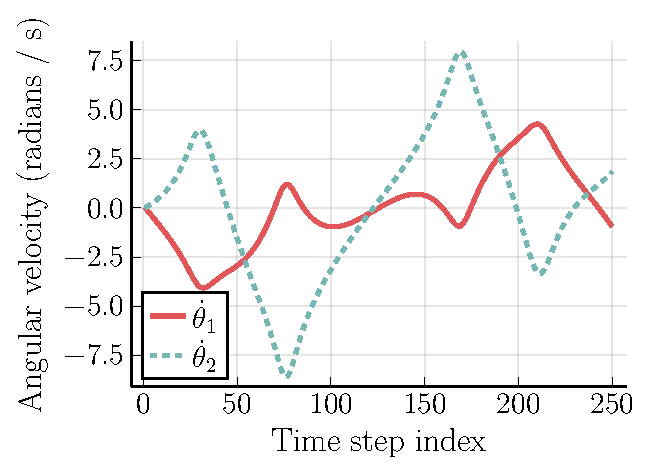
\includegraphics{contents/05-experiments/plots/nlds/03-pendulum_example_velocities.pdf}
    }
    \caption{Simulated evolution of the angular velocities $\dot{\theta}_1$ and $\dot{\theta}_2$ at each time step index $t$.}
    \label{fig:sim:pendulum_example_velocities}
  \end{subfigure}
  \caption{Simulated evolution of the double pendulum system state $s_t = (\theta_1, \theta_2, \dot{\theta}_1, \dot{\theta}_2)_t$ using the Runge-Kutta (RK4) method with a starting point of $s_1 = (1.2, 0.2, 0.0, 0.0)$ in discrete time steps.
    The time difference between measurements is set to be $0.01$ seconds.
    The masses $m_1$ and $m_2$ are set to be $14.715$ and $4.905$ respectively.
    The lengths $l_1$ and $l_2$ are equal and set to be $1.0$.
    The measurements $y$ only include the second component of the state vector.
    Other components of the state vector are not observed.
    The state transition noise $v$ is distributed according to the multivariate Normal
    distribution $\mathcal{N}(0, \Sigma)$, where the covariance matrix $\Sigma$ is a diagonal
    matrix with $10^{-6}$ values on the diagonal.
    The measurement noise signal $w$ is distributed according to the Normal distribution
    $\mathcal{N}(0, \Omega)$, where the variance $\Omega$ is set to be $0.3$.
    The figure shows the first $250$ time steps of the simulation.
  }
  \label{fig:sim:pendulum_example_states}
\end{figure}

%\begin{figure}
%\centering
%\resizebox{0.95\textwidth}{!}{% Recommended preamble:
% \usetikzlibrary{arrows.meta}
% \usetikzlibrary{backgrounds}
% \usepgfplotslibrary{patchplots}
% \usepgfplotslibrary{fillbetween}
% \pgfplotsset{%
%     layers/standard/.define layer set={%
%         background,axis background,axis grid,axis ticks,axis lines,axis tick labels,pre main,main,axis descriptions,axis foreground%
%     }{
%         grid style={/pgfplots/on layer=axis grid},%
%         tick style={/pgfplots/on layer=axis ticks},%
%         axis line style={/pgfplots/on layer=axis lines},%
%         label style={/pgfplots/on layer=axis descriptions},%
%         legend style={/pgfplots/on layer=axis descriptions},%
%         title style={/pgfplots/on layer=axis descriptions},%
%         colorbar style={/pgfplots/on layer=axis descriptions},%
%         ticklabel style={/pgfplots/on layer=axis tick labels},%
%         axis background@ style={/pgfplots/on layer=axis background},%
%         3d box foreground style={/pgfplots/on layer=axis foreground},%
%     },
% }

\begin{tikzpicture}[/tikz/background rectangle/.style={fill={rgb,1:red,1.0;green,1.0;blue,1.0}, fill opacity={1.0}, draw opacity={1.0}}, show background rectangle]
\begin{axis}[point meta max={nan}, point meta min={nan}, legend cell align={left}, legend columns={1}, title={}, title style={at={{(0.5,1)}}, anchor={south}, font={{\fontsize{18 pt}{23.400000000000002 pt}\selectfont}}, color={rgb,1:red,0.0;green,0.0;blue,0.0}, draw opacity={1.0}, rotate={0.0}, align={center}}, legend style={color={rgb,1:red,0.0;green,0.0;blue,0.0}, draw opacity={1.0}, line width={1}, solid, fill={rgb,1:red,1.0;green,1.0;blue,1.0}, fill opacity={1.0}, text opacity={1.0}, font={{\fontsize{16 pt}{20.8 pt}\selectfont}}, text={rgb,1:red,0.0;green,0.0;blue,0.0}, cells={anchor={center}}, at={(0.98, 0.02)}, anchor={south east}}, axis background/.style={fill={rgb,1:red,1.0;green,1.0;blue,1.0}, opacity={1.0}}, anchor={north west}, xshift={1.0mm}, yshift={-1.0mm}, width={201.2mm}, height={74.2mm}, scaled x ticks={false}, xlabel={Time step index}, x tick style={color={rgb,1:red,0.0;green,0.0;blue,0.0}, opacity={1.0}}, x tick label style={color={rgb,1:red,0.0;green,0.0;blue,0.0}, opacity={1.0}, rotate={0}}, xlabel style={at={(ticklabel cs:0.5)}, anchor=near ticklabel, at={{(ticklabel cs:0.5)}}, anchor={near ticklabel}, font={{\fontsize{18 pt}{23.400000000000002 pt}\selectfont}}, color={rgb,1:red,0.0;green,0.0;blue,0.0}, draw opacity={1.0}, rotate={0.0}}, xmajorgrids={true}, xmin={-13.970000000000027}, xmax={514.97}, xticklabels={{$0$,$100$,$200$,$300$,$400$,$500$}}, xtick={{0.0,100.0,200.0,300.0,400.0,500.0}}, xtick align={inside}, xticklabel style={font={{\fontsize{16 pt}{20.8 pt}\selectfont}}, color={rgb,1:red,0.0;green,0.0;blue,0.0}, draw opacity={1.0}, rotate={0.0}}, x grid style={color={rgb,1:red,0.0;green,0.0;blue,0.0}, draw opacity={0.1}, line width={0.5}, solid}, axis x line*={left}, x axis line style={color={rgb,1:red,0.0;green,0.0;blue,0.0}, draw opacity={1.0}, line width={1}, solid}, scaled y ticks={false}, ylabel={Angle (radians)}, y tick style={color={rgb,1:red,0.0;green,0.0;blue,0.0}, opacity={1.0}}, y tick label style={color={rgb,1:red,0.0;green,0.0;blue,0.0}, opacity={1.0}, rotate={0}}, ylabel style={at={(ticklabel cs:0.5)}, anchor=near ticklabel, at={{(ticklabel cs:0.5)}}, anchor={near ticklabel}, font={{\fontsize{18 pt}{23.400000000000002 pt}\selectfont}}, color={rgb,1:red,0.0;green,0.0;blue,0.0}, draw opacity={1.0}, rotate={0.0}}, ymajorgrids={true}, ymin={-3.1627985685809996}, ymax={4.001398297675946}, yticklabels={{$-2$,$0$,$2$,$4$}}, ytick={{-2.0,0.0,2.0,4.0}}, ytick align={inside}, yticklabel style={font={{\fontsize{16 pt}{20.8 pt}\selectfont}}, color={rgb,1:red,0.0;green,0.0;blue,0.0}, draw opacity={1.0}, rotate={0.0}}, y grid style={color={rgb,1:red,0.0;green,0.0;blue,0.0}, draw opacity={0.1}, line width={0.5}, solid}, axis y line*={left}, y axis line style={color={rgb,1:red,0.0;green,0.0;blue,0.0}, draw opacity={1.0}, line width={1}, solid}, colorbar={false}]
    \addplot[color={rgb,1:red,0.349;green,0.6314;blue,0.3098}, name path={20e679cb-e292-4d72-a30f-3c01ec8a30d4}, only marks, draw opacity={1.0}, line width={0}, solid, mark={*}, mark size={1.5 pt}, mark repeat={1}, mark options={color={rgb,1:red,0.0;green,0.0;blue,0.0}, draw opacity={1.0}, fill={rgb,1:red,0.349;green,0.6314;blue,0.3098}, fill opacity={1.0}, line width={0.0}, rotate={0}, solid}]
        table[row sep={\\}]
        {
            \\
            1.0  0.2547037461634025  \\
            2.0  0.13257046233559705  \\
            3.0  -0.03776758991926968  \\
            4.0  0.09161371400759022  \\
            5.0  0.03580303079397851  \\
            6.0  0.5243201219639236  \\
            7.0  -0.8317678104217855  \\
            8.0  0.7337639757938248  \\
            9.0  0.22525926075097388  \\
            10.0  0.060703235270812284  \\
            11.0  1.1737933912733125  \\
            12.0  0.7293091316300014  \\
            13.0  0.4526942096503235  \\
            14.0  0.23733115525947865  \\
            15.0  0.10045711610050653  \\
            16.0  0.010002203005235799  \\
            17.0  0.5849716363761392  \\
            18.0  1.0358206629387468  \\
            19.0  -0.06737686312785268  \\
            20.0  0.8199790894376653  \\
            21.0  0.11075360934320727  \\
            22.0  0.13090376179252466  \\
            23.0  0.6199697498576933  \\
            24.0  0.47159275449181753  \\
            25.0  0.5929405416150995  \\
            26.0  -1.2135665373223106  \\
            27.0  -0.44866295973229275  \\
            28.0  1.3265840688107517  \\
            29.0  -0.36583305536554445  \\
            30.0  0.949304748387459  \\
            31.0  1.1280175834461463  \\
            32.0  -0.18824106990492295  \\
            33.0  1.1197643355571476  \\
            34.0  0.5492803261703256  \\
            35.0  0.7686902631208499  \\
            36.0  0.3711370099283624  \\
            37.0  1.5122590414691222  \\
            38.0  0.6389043165711847  \\
            39.0  1.7274218873887848  \\
            40.0  0.7571412667515867  \\
            41.0  0.8204111857224877  \\
            42.0  0.7358486110893316  \\
            43.0  0.4968958503130323  \\
            44.0  2.5685992967612394  \\
            45.0  1.406056678762214  \\
            46.0  -0.7143217877382071  \\
            47.0  1.4991134982528218  \\
            48.0  0.46361233396621204  \\
            49.0  -0.10732966757856954  \\
            50.0  0.005352002113944487  \\
            51.0  0.4302888807554356  \\
            52.0  1.7421359411792186  \\
            53.0  1.8204722216757916  \\
            54.0  2.4952368321404834  \\
            55.0  1.3370275881377172  \\
            56.0  0.3529439649780819  \\
            57.0  0.33008697408953047  \\
            58.0  0.6228590344824246  \\
            59.0  0.6456893503624443  \\
            60.0  -0.03454432042297306  \\
            61.0  1.3902048320595508  \\
            62.0  0.3946371884144047  \\
            63.0  -0.5108757055489302  \\
            64.0  -0.3413719851201213  \\
            65.0  0.11345939121094634  \\
            66.0  -0.06852280893165702  \\
            67.0  1.042928613543596  \\
            68.0  0.016429464666352145  \\
            69.0  -0.6325896533488691  \\
            70.0  0.7132531520286924  \\
            71.0  -0.2589576993379058  \\
            72.0  -0.3270350833595384  \\
            73.0  -0.9987946037390639  \\
            74.0  0.08700004838123115  \\
            75.0  -0.8414776367231596  \\
            76.0  -0.9661575945971216  \\
            77.0  -0.3973354477736911  \\
            78.0  -0.9612560502306002  \\
            79.0  -0.10336496442805954  \\
            80.0  -0.09609815268853472  \\
            81.0  -1.1592087786938123  \\
            82.0  -1.752612003763668  \\
            83.0  -1.1469312919276016  \\
            84.0  -0.47904067512064585  \\
            85.0  0.10934428785343453  \\
            86.0  -1.1814654323630396  \\
            87.0  -1.7847524419801517  \\
            88.0  -1.0446277627615885  \\
            89.0  -1.8202833045766815  \\
            90.0  -1.3618410397311158  \\
            91.0  -1.6615797777525465  \\
            92.0  -0.20041513781277365  \\
            93.0  -1.8066344946051562  \\
            94.0  -1.9973256250305298  \\
            95.0  -1.5276086342422077  \\
            96.0  -1.9069607291602308  \\
            97.0  -2.283888732889661  \\
            98.0  -1.7495055467102847  \\
            99.0  -1.280413978460448  \\
            100.0  -1.794527938788751  \\
            101.0  -0.9350793519095448  \\
            102.0  -1.7801702059944355  \\
            103.0  -1.3307663563417451  \\
            104.0  -2.4753523322202415  \\
            105.0  -1.405132012217344  \\
            106.0  -1.2928011724102173  \\
            107.0  -1.6083470684035137  \\
            108.0  -1.6917811864631256  \\
            109.0  -1.120361859962426  \\
            110.0  -2.030965288679942  \\
            111.0  -2.242777682861987  \\
            112.0  -1.6518689048681314  \\
            113.0  -2.2793768057160637  \\
            114.0  -1.8821228665101208  \\
            115.0  -2.6957631794674164  \\
            116.0  -1.7461509806630824  \\
            117.0  -2.1419322564559584  \\
            118.0  -2.9600382799133507  \\
            119.0  -1.549348642096706  \\
            120.0  -1.7786924083727553  \\
            121.0  -2.279279300137501  \\
            122.0  -1.4197770384800101  \\
            123.0  -2.4870009676186786  \\
            124.0  -1.8939187940668558  \\
            125.0  -1.1452780024184255  \\
            126.0  -1.762804657436483  \\
            127.0  -2.958358586447785  \\
            128.0  -1.9678753036282253  \\
            129.0  -1.2866120734788664  \\
            130.0  -2.6288486206158783  \\
            131.0  -2.1318523277248858  \\
            132.0  -1.6020497590171445  \\
            133.0  -1.9787588277831722  \\
            134.0  -1.1479390192078547  \\
            135.0  -1.265486139945545  \\
            136.0  -2.1802697522359984  \\
            137.0  -1.9517398595235642  \\
            138.0  -1.7475681174680806  \\
            139.0  -1.9833710265259836  \\
            140.0  -2.1490718382039655  \\
            141.0  -1.3291352355050958  \\
            142.0  -1.743851573349185  \\
            143.0  -1.3600481155221495  \\
            144.0  -1.7714493216840912  \\
            145.0  -0.8962415563893462  \\
            146.0  -0.8234230389913816  \\
            147.0  -2.324907308996061  \\
            148.0  -1.254133825881493  \\
            149.0  -1.6097525414786458  \\
            150.0  -0.578114139934352  \\
            151.0  -1.3239620059485115  \\
            152.0  -0.7243928919061647  \\
            153.0  -1.283410064621941  \\
            154.0  -1.7473270629033948  \\
            155.0  -0.6986673644819154  \\
            156.0  -1.8626151500844275  \\
            157.0  -1.9347445137447257  \\
            158.0  -0.842063234393021  \\
            159.0  -2.05895557547552  \\
            160.0  -1.0435751654902805  \\
            161.0  -2.021011187277641  \\
            162.0  0.04549998660082011  \\
            163.0  -0.792534551761701  \\
            164.0  -0.9068480486991035  \\
            165.0  -0.2262425834735241  \\
            166.0  -0.9518746721201454  \\
            167.0  -0.22718942854916757  \\
            168.0  -0.08412107533518237  \\
            169.0  -1.3775567238188153  \\
            170.0  -0.5773270441455716  \\
            171.0  0.4548574286780537  \\
            172.0  -0.4913342999311329  \\
            173.0  -1.5196404104094683  \\
            174.0  0.04670881449122884  \\
            175.0  -0.03981830747880498  \\
            176.0  -0.03051172022122728  \\
            177.0  -0.7666882010123338  \\
            178.0  -0.8514670831496012  \\
            179.0  -0.31112845208766404  \\
            180.0  0.23461705449331224  \\
            181.0  -0.5667738317603577  \\
            182.0  0.3957519902448624  \\
            183.0  0.7909567080577389  \\
            184.0  0.35341347958062397  \\
            185.0  1.1364681196456983  \\
            186.0  -0.8866984983949993  \\
            187.0  0.8355489057574816  \\
            188.0  1.4286726142240131  \\
            189.0  0.6967053593922535  \\
            190.0  0.13057315453066154  \\
            191.0  0.003951425711167467  \\
            192.0  0.12893881621325853  \\
            193.0  0.3418514828675006  \\
            194.0  0.6623690670745918  \\
            195.0  0.971115257437804  \\
            196.0  0.8675616707231275  \\
            197.0  1.659762788216834  \\
            198.0  -0.22980701221832445  \\
            199.0  0.8158018319882907  \\
            200.0  1.1128360472584942  \\
            201.0  -0.29601005369727285  \\
            202.0  0.7023766852736714  \\
            203.0  0.9293406180086811  \\
            204.0  0.29015371371690346  \\
            205.0  0.7556310056529474  \\
            206.0  1.4344105171084804  \\
            207.0  1.4698620035432237  \\
            208.0  1.2941818852525873  \\
            209.0  0.3176034193205455  \\
            210.0  0.6785517639346975  \\
            211.0  0.792172500328094  \\
            212.0  1.2646419707916983  \\
            213.0  0.7960149273348547  \\
            214.0  0.3152646318989692  \\
            215.0  0.6548741529538871  \\
            216.0  -0.21144910077212714  \\
            217.0  -0.19414924581320875  \\
            218.0  -0.4740329810364304  \\
            219.0  0.9927697879645445  \\
            220.0  0.7241107825685815  \\
            221.0  1.6116659856676383  \\
            222.0  0.1350016249205366  \\
            223.0  0.6073804642947458  \\
            224.0  -0.6440673069791236  \\
            225.0  0.28335334619370584  \\
            226.0  0.35746396362649174  \\
            227.0  -0.4721405871607463  \\
            228.0  0.31718158750288894  \\
            229.0  0.9034357373574358  \\
            230.0  0.4162164899549826  \\
            231.0  0.6785569721554142  \\
            232.0  -0.7554189124192134  \\
            233.0  -0.07352504380112157  \\
            234.0  0.4799551408175747  \\
            235.0  0.6111606993526726  \\
            236.0  0.8035344971127392  \\
            237.0  0.4172396951092041  \\
            238.0  0.2264966528743171  \\
            239.0  -0.9837931596618397  \\
            240.0  0.49360922876195135  \\
            241.0  -0.20391346638707497  \\
            242.0  -0.04427114824239464  \\
            243.0  0.5320992830720863  \\
            244.0  0.7547897166086556  \\
            245.0  0.12664982304599093  \\
            246.0  -0.25291909862300027  \\
            247.0  0.05474471648881557  \\
            248.0  0.7012705881732797  \\
            249.0  1.1126540575872577  \\
            250.0  0.9564509782059143  \\
            251.0  0.6086049342251145  \\
            252.0  0.36497917307272715  \\
            253.0  0.8107120223693237  \\
            254.0  -0.14022250368494682  \\
            255.0  -0.5567382267815906  \\
            256.0  2.042790666922171  \\
            257.0  0.28553466984456144  \\
            258.0  1.0556365973219524  \\
            259.0  0.34777014128007483  \\
            260.0  -0.18067156125584405  \\
            261.0  1.997332567858869  \\
            262.0  1.684860640174111  \\
            263.0  0.12781814933239244  \\
            264.0  0.9343981681768515  \\
            265.0  0.8918032967660761  \\
            266.0  0.46063174159636844  \\
            267.0  0.7148957229897894  \\
            268.0  0.8443678383635875  \\
            269.0  0.8841012329654054  \\
            270.0  1.595037634437785  \\
            271.0  0.9208737925369979  \\
            272.0  1.706996691692529  \\
            273.0  2.2546304108994804  \\
            274.0  2.0122559426806443  \\
            275.0  1.3866010921131795  \\
            276.0  0.4660724748335717  \\
            277.0  1.6597815170707642  \\
            278.0  2.1037716408757894  \\
            279.0  1.0953964595497925  \\
            280.0  1.5607946722551016  \\
            281.0  0.9414944402504257  \\
            282.0  0.5607578326192387  \\
            283.0  1.4278986129947961  \\
            284.0  2.076966846601141  \\
            285.0  1.3999069772729673  \\
            286.0  0.8150626347309256  \\
            287.0  0.5485022388438334  \\
            288.0  1.5059141464901211  \\
            289.0  0.7290835898276607  \\
            290.0  1.6049076623581637  \\
            291.0  1.5697447834792064  \\
            292.0  0.45171024839277607  \\
            293.0  0.8293124007853085  \\
            294.0  0.846601310395398  \\
            295.0  0.8739146920926135  \\
            296.0  0.08488410227529886  \\
            297.0  0.002190553834938269  \\
            298.0  0.5598896749165143  \\
            299.0  0.6488627031233556  \\
            300.0  0.6626201431943712  \\
            301.0  1.550809263129851  \\
            302.0  1.2035366486807428  \\
            303.0  1.4391513598957628  \\
            304.0  0.9465325080806437  \\
            305.0  1.0363051989532819  \\
            306.0  0.23808535182725732  \\
            307.0  0.6627634639145569  \\
            308.0  0.07281148228098394  \\
            309.0  -0.5777034836980899  \\
            310.0  -0.12292021554616031  \\
            311.0  1.0502619194373501  \\
            312.0  -0.45659941413233857  \\
            313.0  0.15183854869504282  \\
            314.0  -0.6863180564401987  \\
            315.0  0.3230755997005984  \\
            316.0  -0.9453184589914141  \\
            317.0  -0.4585674228477514  \\
            318.0  -1.3071798370154104  \\
            319.0  -0.4978799443024999  \\
            320.0  -0.4088673706448102  \\
            321.0  -0.3128210562588147  \\
            322.0  -1.146473803498684  \\
            323.0  -0.7587892155610564  \\
            324.0  -1.4263939872180178  \\
            325.0  -0.7074078532701644  \\
            326.0  -1.022633900769508  \\
            327.0  -0.98774822932522  \\
            328.0  -0.6916193332964828  \\
            329.0  -2.0016733429279228  \\
            330.0  -1.4131814744671165  \\
            331.0  -1.7930584486992707  \\
            332.0  -1.0855561768133115  \\
            333.0  -1.7393989295487908  \\
            334.0  -1.3819726354505815  \\
            335.0  -1.1648785058254565  \\
            336.0  -1.1696073623634942  \\
            337.0  -2.22389591886838  \\
            338.0  -1.436309384075033  \\
            339.0  -1.4251929505875185  \\
            340.0  -2.776049799437655  \\
            341.0  -2.015551359451244  \\
            342.0  -1.4453997369175922  \\
            343.0  -1.6318896644401617  \\
            344.0  -1.3405557295883137  \\
            345.0  -1.938032837095029  \\
            346.0  -1.1602399262184786  \\
            347.0  -2.2341320955057733  \\
            348.0  -2.023659457762066  \\
            349.0  -1.3512464239084263  \\
            350.0  -1.2546849565308018  \\
            351.0  -2.789860757175241  \\
            352.0  -2.1450923087806646  \\
            353.0  -1.4082746958849548  \\
            354.0  -2.124991790703219  \\
            355.0  -2.524805156615292  \\
            356.0  -1.3570631992843396  \\
            357.0  -2.1583761447926655  \\
            358.0  -1.4119514670359934  \\
            359.0  -2.6025322083758513  \\
            360.0  -2.2737146590008903  \\
            361.0  -0.9001825844007502  \\
            362.0  -1.573369654329728  \\
            363.0  -0.599429902944882  \\
            364.0  -1.4189348800495303  \\
            365.0  -1.4594283988176981  \\
            366.0  -1.442131238522419  \\
            367.0  -1.9203528374277246  \\
            368.0  -2.163109350493304  \\
            369.0  -1.6720797183679454  \\
            370.0  -2.3683604047124254  \\
            371.0  -1.8192560001767353  \\
            372.0  -1.8596849452131368  \\
            373.0  -2.133720376870821  \\
            374.0  -2.1572688262127735  \\
            375.0  -2.0132201429760843  \\
            376.0  -2.251616277999592  \\
            377.0  -1.6512530881801881  \\
            378.0  -2.5752184245881256  \\
            379.0  -1.4988184096798005  \\
            380.0  -1.5770600580654228  \\
            381.0  -1.4176315937500161  \\
            382.0  -0.3842147119966244  \\
            383.0  -1.3145227316277073  \\
            384.0  -1.5181413561303954  \\
            385.0  -0.9843052329262914  \\
            386.0  -1.3493778679300799  \\
            387.0  -0.8600089106646416  \\
            388.0  -0.9397972935597814  \\
            389.0  -1.647682186971911  \\
            390.0  -0.24146190170522108  \\
            391.0  -1.149427215835684  \\
            392.0  -0.6135056898672351  \\
            393.0  -0.23704227857604454  \\
            394.0  -0.7266293222284332  \\
            395.0  -0.6469705578152578  \\
            396.0  -0.3302973842437824  \\
            397.0  0.026955363776290597  \\
            398.0  -0.6066017396824744  \\
            399.0  -0.28600718047321994  \\
            400.0  -0.4411287947197255  \\
            401.0  -0.8407578459391283  \\
            402.0  -0.8566991229381864  \\
            403.0  -0.11663955661405484  \\
            404.0  -0.2318327999287174  \\
            405.0  -1.3079709713328675  \\
            406.0  -0.373487161529459  \\
            407.0  -0.7188321977668082  \\
            408.0  -0.23123651433818074  \\
            409.0  -0.1856290459735493  \\
            410.0  -0.540336242094907  \\
            411.0  0.8337033209990051  \\
            412.0  -0.3396091540246816  \\
            413.0  -0.42910998394416744  \\
            414.0  -0.09462292850916931  \\
            415.0  -0.15017075721075504  \\
            416.0  0.41213988117037437  \\
            417.0  0.36491289243153135  \\
            418.0  0.337896049834181  \\
            419.0  -0.14159182180049262  \\
            420.0  0.3100023522725418  \\
            421.0  -0.15411792005010652  \\
            422.0  -0.04805806938270364  \\
            423.0  -0.1694380388120736  \\
            424.0  -0.20075377742702127  \\
            425.0  -0.008950829491479642  \\
            426.0  -0.4149538639880728  \\
            427.0  0.1315005462593218  \\
            428.0  -0.0978205171395651  \\
            429.0  -0.32781175892481035  \\
            430.0  -0.5416378726445532  \\
            431.0  -0.592027995888375  \\
            432.0  -0.0072412499821009335  \\
            433.0  1.0757461134062702  \\
            434.0  0.3187614023975534  \\
            435.0  -0.3462311843273594  \\
            436.0  0.7877353816789289  \\
            437.0  0.6063977877619431  \\
            438.0  -0.6253099371736408  \\
            439.0  -0.5251760267252457  \\
            440.0  -0.7042190087360131  \\
            441.0  0.501730289547447  \\
            442.0  -0.5432339546632522  \\
            443.0  0.46240715276019245  \\
            444.0  -1.3638831432538736  \\
            445.0  0.27692021444472936  \\
            446.0  -0.28368394816613585  \\
            447.0  0.03578460381578301  \\
            448.0  -0.22517247272992194  \\
            449.0  -0.5598223791153143  \\
            450.0  1.2340688123060086  \\
            451.0  0.7872944419691128  \\
            452.0  0.2722569244292567  \\
            453.0  0.4254568179708278  \\
            454.0  0.1969275217683756  \\
            455.0  1.133441032672545  \\
            456.0  0.6658599460644867  \\
            457.0  1.9985518620530995  \\
            458.0  0.016524650050032896  \\
            459.0  0.807295983156374  \\
            460.0  0.7250361007337011  \\
            461.0  0.5332407655761877  \\
            462.0  -0.7119212761095042  \\
            463.0  2.4026773260289414  \\
            464.0  0.029620102395093495  \\
            465.0  0.7926953815630983  \\
            466.0  2.0601968140143283  \\
            467.0  0.5597883347518665  \\
            468.0  0.2514432720609753  \\
            469.0  0.6302679706671976  \\
            470.0  1.108173209534797  \\
            471.0  0.8255730143149258  \\
            472.0  1.3672865928237867  \\
            473.0  2.127190053908513  \\
            474.0  0.7028778760573932  \\
            475.0  1.0740457652865356  \\
            476.0  1.3401585553280866  \\
            477.0  1.3221688074315678  \\
            478.0  2.0436794384366976  \\
            479.0  1.504102864120624  \\
            480.0  1.680958305960178  \\
            481.0  1.1510945551751592  \\
            482.0  1.0373728076856932  \\
            483.0  0.9736528078858427  \\
            484.0  2.323150574619187  \\
            485.0  1.6585870925096187  \\
            486.0  1.4809574354758377  \\
            487.0  0.4707693339277854  \\
            488.0  1.7715124020594613  \\
            489.0  2.2854953468975143  \\
            490.0  1.4861928161488789  \\
            491.0  1.5555742747797223  \\
            492.0  1.842983651332346  \\
            493.0  3.7986380090082967  \\
            494.0  2.6034814916128366  \\
            495.0  2.6757511607228572  \\
            496.0  1.6688285847992965  \\
            497.0  2.2405816958585785  \\
            498.0  1.9152722958693746  \\
            499.0  1.7944875204012671  \\
            500.0  1.960266375197512  \\
        }
        ;
    \addlegendentry {$y = \theta_2 + \omega$}
    \addplot[color={rgb,1:red,0.949;green,0.5569;blue,0.1686}, name path={d5feaefa-7394-43f6-b2be-5a8419165467}, draw opacity={1.0}, line width={2}, dashed]
        table[row sep={\\}]
        {
            \\
            1.0  0.2  \\
            2.0  0.20077121306979956  \\
            3.0  0.20244421310869218  \\
            4.0  0.20538450261381772  \\
            5.0  0.2076748169724466  \\
            6.0  0.21004613114216075  \\
            7.0  0.21198732109905916  \\
            8.0  0.21872872777404256  \\
            9.0  0.22323289221781725  \\
            10.0  0.22943985449754048  \\
            11.0  0.23581566502370901  \\
            12.0  0.24315735276246045  \\
            13.0  0.25284533768152134  \\
            14.0  0.26333740397862243  \\
            15.0  0.2767267762686036  \\
            16.0  0.29025284273577634  \\
            17.0  0.30537834643258177  \\
            18.0  0.3223457673611555  \\
            19.0  0.33790075820583876  \\
            20.0  0.35864484846938993  \\
            21.0  0.381008210128867  \\
            22.0  0.40503304101881643  \\
            23.0  0.4297012844324011  \\
            24.0  0.45813855895874606  \\
            25.0  0.48682693931483995  \\
            26.0  0.5206129038195051  \\
            27.0  0.5559471357422973  \\
            28.0  0.5922734827511258  \\
            29.0  0.6295904162401603  \\
            30.0  0.6681568582309619  \\
            31.0  0.7069617380962739  \\
            32.0  0.7458108999643405  \\
            33.0  0.7837109003387867  \\
            34.0  0.8199399855636275  \\
            35.0  0.8502841255822313  \\
            36.0  0.8783688485478693  \\
            37.0  0.9035997250689355  \\
            38.0  0.9251420935601686  \\
            39.0  0.9447342773893882  \\
            40.0  0.9621520056848557  \\
            41.0  0.9766089837799784  \\
            42.0  0.9890431780302547  \\
            43.0  0.9949241636544784  \\
            44.0  0.9969713618207969  \\
            45.0  0.9973295439251917  \\
            46.0  0.9932927022359279  \\
            47.0  0.9864562676330484  \\
            48.0  0.9780658607032465  \\
            49.0  0.9663855710137768  \\
            50.0  0.9536149015339549  \\
            51.0  0.9353859590904313  \\
            52.0  0.9147743221649417  \\
            53.0  0.8924033613981605  \\
            54.0  0.8670071208395579  \\
            55.0  0.8401128720204886  \\
            56.0  0.80859996527425  \\
            57.0  0.7750602396433758  \\
            58.0  0.7390795630859462  \\
            59.0  0.700158369569577  \\
            60.0  0.6588167666960625  \\
            61.0  0.6137401324392603  \\
            62.0  0.5654269061868354  \\
            63.0  0.5151341678076061  \\
            64.0  0.46252447496209453  \\
            65.0  0.40651420138940986  \\
            66.0  0.3505493080310132  \\
            67.0  0.2921725223792161  \\
            68.0  0.23005615438543553  \\
            69.0  0.16228513577315584  \\
            70.0  0.09250511552723756  \\
            71.0  0.019513296113997818  \\
            72.0  -0.057542073684514736  \\
            73.0  -0.137917451369763  \\
            74.0  -0.21952606427583504  \\
            75.0  -0.30457893498341554  \\
            76.0  -0.3915912846654537  \\
            77.0  -0.47728396192190414  \\
            78.0  -0.5636963639110109  \\
            79.0  -0.6444670567618447  \\
            80.0  -0.7239413402630823  \\
            81.0  -0.7989819317719744  \\
            82.0  -0.8715307328990217  \\
            83.0  -0.940233108432891  \\
            84.0  -1.005239787419807  \\
            85.0  -1.0685953502753918  \\
            86.0  -1.1283227352474465  \\
            87.0  -1.185359026976821  \\
            88.0  -1.2394906751023496  \\
            89.0  -1.2943304148202577  \\
            90.0  -1.3441062924771507  \\
            91.0  -1.3902859791631426  \\
            92.0  -1.4366803682827065  \\
            93.0  -1.4811529284215403  \\
            94.0  -1.5225448964617248  \\
            95.0  -1.563730261262378  \\
            96.0  -1.5997131249515735  \\
            97.0  -1.6366441866414128  \\
            98.0  -1.6733136776466513  \\
            99.0  -1.7056024983702138  \\
            100.0  -1.737847797377272  \\
            101.0  -1.768615713947156  \\
            102.0  -1.7973953650595775  \\
            103.0  -1.8266478016459915  \\
            104.0  -1.8525142454289871  \\
            105.0  -1.875355680191903  \\
            106.0  -1.8985285772418155  \\
            107.0  -1.9200193226034352  \\
            108.0  -1.9382098190965413  \\
            109.0  -1.955117629532639  \\
            110.0  -1.9696443312177885  \\
            111.0  -1.9839163127155266  \\
            112.0  -1.9971876830609512  \\
            113.0  -2.010110211562051  \\
            114.0  -2.0209182957170873  \\
            115.0  -2.0325631009319194  \\
            116.0  -2.0404197873851406  \\
            117.0  -2.047105285757217  \\
            118.0  -2.05406118715393  \\
            119.0  -2.0578465063172775  \\
            120.0  -2.061754863949012  \\
            121.0  -2.0623956324894124  \\
            122.0  -2.0635020145097647  \\
            123.0  -2.065016572927728  \\
            124.0  -2.0642986961816012  \\
            125.0  -2.062082836640928  \\
            126.0  -2.0572354604704226  \\
            127.0  -2.051457063599901  \\
            128.0  -2.0453135650132035  \\
            129.0  -2.0377082511655993  \\
            130.0  -2.0271684177566027  \\
            131.0  -2.0174163118592103  \\
            132.0  -2.006627255161083  \\
            133.0  -1.99458661776932  \\
            134.0  -1.981714592694915  \\
            135.0  -1.9657357644053175  \\
            136.0  -1.95008811649449  \\
            137.0  -1.9303573794981208  \\
            138.0  -1.9110237806162047  \\
            139.0  -1.891032236293788  \\
            140.0  -1.86892276396149  \\
            141.0  -1.8459024476627526  \\
            142.0  -1.8240516541245848  \\
            143.0  -1.7969981244184352  \\
            144.0  -1.7689196262694191  \\
            145.0  -1.7410262603456275  \\
            146.0  -1.7107785978513035  \\
            147.0  -1.6775932275228054  \\
            148.0  -1.6435335559227948  \\
            149.0  -1.6087777293433998  \\
            150.0  -1.5715761528918881  \\
            151.0  -1.5333355225829213  \\
            152.0  -1.4924470485598136  \\
            153.0  -1.4505696989582664  \\
            154.0  -1.4081074652001293  \\
            155.0  -1.3631752509782977  \\
            156.0  -1.315047608485016  \\
            157.0  -1.2671404222558629  \\
            158.0  -1.2145856333462213  \\
            159.0  -1.1590012892917456  \\
            160.0  -1.1007170055946283  \\
            161.0  -1.0412272270808436  \\
            162.0  -0.9788028842153407  \\
            163.0  -0.9154362282771672  \\
            164.0  -0.8467195634224802  \\
            165.0  -0.7740772228420397  \\
            166.0  -0.6991025525069955  \\
            167.0  -0.6219897733785096  \\
            168.0  -0.544075776265649  \\
            169.0  -0.4647533959092831  \\
            170.0  -0.3871719296897495  \\
            171.0  -0.30871861039755644  \\
            172.0  -0.23228660994473999  \\
            173.0  -0.16006993457316293  \\
            174.0  -0.09104079554576809  \\
            175.0  -0.023836038553904634  \\
            176.0  0.04065941764398388  \\
            177.0  0.10298433719679366  \\
            178.0  0.16191786460486846  \\
            179.0  0.21717664729431627  \\
            180.0  0.27196657770121696  \\
            181.0  0.32217097417301116  \\
            182.0  0.3704057719112007  \\
            183.0  0.41381936139150055  \\
            184.0  0.45562076321800266  \\
            185.0  0.4956701607299468  \\
            186.0  0.533427051320366  \\
            187.0  0.568639337023961  \\
            188.0  0.6009351087159419  \\
            189.0  0.6309386763830759  \\
            190.0  0.6559845555974834  \\
            191.0  0.6807106299250723  \\
            192.0  0.702832881211831  \\
            193.0  0.7215784638941529  \\
            194.0  0.7368913573391841  \\
            195.0  0.7489647617236266  \\
            196.0  0.7587190342979474  \\
            197.0  0.7647364823399241  \\
            198.0  0.7678485327456598  \\
            199.0  0.7664416622206628  \\
            200.0  0.7638649055908637  \\
            201.0  0.7571631057135545  \\
            202.0  0.7459260731431627  \\
            203.0  0.7330132005437374  \\
            204.0  0.7166998253727788  \\
            205.0  0.6970059767715231  \\
            206.0  0.6728385877341402  \\
            207.0  0.6478060532225469  \\
            208.0  0.6195863531767273  \\
            209.0  0.5868529561778992  \\
            210.0  0.5565162004508684  \\
            211.0  0.5235131226371783  \\
            212.0  0.49046125601779067  \\
            213.0  0.45908445524916563  \\
            214.0  0.4287847959908928  \\
            215.0  0.3998148291027864  \\
            216.0  0.37347240850929825  \\
            217.0  0.3480287471251013  \\
            218.0  0.3267248542670755  \\
            219.0  0.30876219079313677  \\
            220.0  0.29228402246562163  \\
            221.0  0.27752050815829726  \\
            222.0  0.2665193975217233  \\
            223.0  0.2587725529804194  \\
            224.0  0.2529307282775175  \\
            225.0  0.2483180748127668  \\
            226.0  0.2440885148853471  \\
            227.0  0.2427798059909984  \\
            228.0  0.2426666754505097  \\
            229.0  0.24357407307853082  \\
            230.0  0.24644402757467024  \\
            231.0  0.24939693899033108  \\
            232.0  0.2543840911518738  \\
            233.0  0.2601560785761774  \\
            234.0  0.2675938233072742  \\
            235.0  0.2761793284140923  \\
            236.0  0.2849108055903707  \\
            237.0  0.29213702863752405  \\
            238.0  0.30335718171378145  \\
            239.0  0.31517148765300046  \\
            240.0  0.3259089236880202  \\
            241.0  0.3399682838979915  \\
            242.0  0.352352226201167  \\
            243.0  0.36610976576424914  \\
            244.0  0.3811338156002569  \\
            245.0  0.39720331331081  \\
            246.0  0.41544809635028374  \\
            247.0  0.4342584566805917  \\
            248.0  0.45318580254310387  \\
            249.0  0.47051640079546203  \\
            250.0  0.4909670906812182  \\
            251.0  0.5123169411543128  \\
            252.0  0.5341537477526385  \\
            253.0  0.5573820680188972  \\
            254.0  0.5835830581812941  \\
            255.0  0.6107251247397203  \\
            256.0  0.6406161162667461  \\
            257.0  0.6702865430626567  \\
            258.0  0.7016032452233902  \\
            259.0  0.7347960859908554  \\
            260.0  0.7705628308338417  \\
            261.0  0.8059160272118696  \\
            262.0  0.84288803856595  \\
            263.0  0.8811221824524031  \\
            264.0  0.9198144901495555  \\
            265.0  0.95884434700868  \\
            266.0  0.9954583838804504  \\
            267.0  1.0298741377702962  \\
            268.0  1.0620963085025146  \\
            269.0  1.0939848148453273  \\
            270.0  1.1237094248280324  \\
            271.0  1.1499473336236519  \\
            272.0  1.1762164321933248  \\
            273.0  1.19810910993671  \\
            274.0  1.216592320085004  \\
            275.0  1.2340240970896694  \\
            276.0  1.2490729120116455  \\
            277.0  1.2616507087092939  \\
            278.0  1.2731459764365671  \\
            279.0  1.2790286057274227  \\
            280.0  1.2826761038801717  \\
            281.0  1.2818506515993286  \\
            282.0  1.2821127224324627  \\
            283.0  1.2780850357853335  \\
            284.0  1.271882537167133  \\
            285.0  1.2634332162823554  \\
            286.0  1.2525107018951074  \\
            287.0  1.2381118944893745  \\
            288.0  1.2226291302564298  \\
            289.0  1.2041263887955536  \\
            290.0  1.1820500585997478  \\
            291.0  1.1576983384623114  \\
            292.0  1.1307560022316532  \\
            293.0  1.1024438194823365  \\
            294.0  1.071669706706363  \\
            295.0  1.0368412239102822  \\
            296.0  0.9992564558933096  \\
            297.0  0.9611198859474601  \\
            298.0  0.9206250823234695  \\
            299.0  0.8754309651938195  \\
            300.0  0.8296117610952934  \\
            301.0  0.7816644017332739  \\
            302.0  0.7304266423142528  \\
            303.0  0.6756067306473944  \\
            304.0  0.6190265780459794  \\
            305.0  0.5584983854187708  \\
            306.0  0.4945959772946861  \\
            307.0  0.42809256646303506  \\
            308.0  0.35743390304190054  \\
            309.0  0.28237060763882155  \\
            310.0  0.20635408477251946  \\
            311.0  0.1250553670513947  \\
            312.0  0.04180154609516395  \\
            313.0  -0.04551155106840756  \\
            314.0  -0.1345143377334055  \\
            315.0  -0.22336764701950043  \\
            316.0  -0.3125542934537056  \\
            317.0  -0.4006237103481264  \\
            318.0  -0.48579671222006027  \\
            319.0  -0.5661325834512474  \\
            320.0  -0.6426821090518738  \\
            321.0  -0.7172673894809637  \\
            322.0  -0.7873213024989413  \\
            323.0  -0.8535899716351228  \\
            324.0  -0.9169131725885248  \\
            325.0  -0.9763768999174139  \\
            326.0  -1.0338852035448125  \\
            327.0  -1.0891228139966511  \\
            328.0  -1.1416932335586711  \\
            329.0  -1.193887252163816  \\
            330.0  -1.2430722378361234  \\
            331.0  -1.2883536780403297  \\
            332.0  -1.329396889152606  \\
            333.0  -1.3721015380533579  \\
            334.0  -1.410587058006288  \\
            335.0  -1.4492797618722968  \\
            336.0  -1.486674589986813  \\
            337.0  -1.5206389114801222  \\
            338.0  -1.5501233600278685  \\
            339.0  -1.5796125431703836  \\
            340.0  -1.605352478506891  \\
            341.0  -1.6305648993554678  \\
            342.0  -1.6556095801916717  \\
            343.0  -1.6776966573688799  \\
            344.0  -1.6997700496991055  \\
            345.0  -1.7191881263115145  \\
            346.0  -1.7369253843635197  \\
            347.0  -1.7515632743001506  \\
            348.0  -1.7643092546648584  \\
            349.0  -1.7755572892747071  \\
            350.0  -1.7858686698589785  \\
            351.0  -1.7934184436420966  \\
            352.0  -1.7990947955853844  \\
            353.0  -1.8028736089432493  \\
            354.0  -1.8053315454855539  \\
            355.0  -1.8079919924695234  \\
            356.0  -1.8093904029978138  \\
            357.0  -1.8078166392243034  \\
            358.0  -1.8055371340062794  \\
            359.0  -1.8019405037544185  \\
            360.0  -1.794975486009442  \\
            361.0  -1.7905792287527662  \\
            362.0  -1.7827217879847146  \\
            363.0  -1.772925501738634  \\
            364.0  -1.7632655353784426  \\
            365.0  -1.7520106091188579  \\
            366.0  -1.7383000493614214  \\
            367.0  -1.7234026804900597  \\
            368.0  -1.708974424622292  \\
            369.0  -1.69236497220162  \\
            370.0  -1.6755435472232991  \\
            371.0  -1.6571146092150943  \\
            372.0  -1.6374132718613716  \\
            373.0  -1.6163102211069915  \\
            374.0  -1.5929513801862383  \\
            375.0  -1.5687634294720114  \\
            376.0  -1.5428182225696192  \\
            377.0  -1.514806187896199  \\
            378.0  -1.4864729695322472  \\
            379.0  -1.4598740006553625  \\
            380.0  -1.428238813862558  \\
            381.0  -1.3966106475504818  \\
            382.0  -1.3633237176332025  \\
            383.0  -1.3297460029459516  \\
            384.0  -1.2927014569083286  \\
            385.0  -1.2559255313171707  \\
            386.0  -1.2176065190303096  \\
            387.0  -1.177734348758448  \\
            388.0  -1.1380828389474167  \\
            389.0  -1.0965241030332809  \\
            390.0  -1.0544048855806913  \\
            391.0  -1.0104318668487824  \\
            392.0  -0.9668637422171491  \\
            393.0  -0.9210986512713824  \\
            394.0  -0.8759473281918401  \\
            395.0  -0.8308703080506649  \\
            396.0  -0.7879880374857822  \\
            397.0  -0.7426043444842876  \\
            398.0  -0.6983254732221218  \\
            399.0  -0.6550811625572704  \\
            400.0  -0.6132201649598005  \\
            401.0  -0.5706226728514276  \\
            402.0  -0.5322993731682073  \\
            403.0  -0.49292381085620945  \\
            404.0  -0.4577807272342732  \\
            405.0  -0.4229313927409816  \\
            406.0  -0.38872015090073975  \\
            407.0  -0.35614586208550836  \\
            408.0  -0.32391746151118594  \\
            409.0  -0.2961991504149649  \\
            410.0  -0.2688703373225751  \\
            411.0  -0.24300339968906806  \\
            412.0  -0.21841312482110195  \\
            413.0  -0.195745558629374  \\
            414.0  -0.1758067598105461  \\
            415.0  -0.15669856498070192  \\
            416.0  -0.14225439628330064  \\
            417.0  -0.1296002340183511  \\
            418.0  -0.1183458774384559  \\
            419.0  -0.10776289230030738  \\
            420.0  -0.09928133750765428  \\
            421.0  -0.09505392176962664  \\
            422.0  -0.0907450575845551  \\
            423.0  -0.0875819912094041  \\
            424.0  -0.08625446621392481  \\
            425.0  -0.08602303669183034  \\
            426.0  -0.08713274729147846  \\
            427.0  -0.08967431522213234  \\
            428.0  -0.09140430098031307  \\
            429.0  -0.09296106125317692  \\
            430.0  -0.09622687805733805  \\
            431.0  -0.09684639699937946  \\
            432.0  -0.09642500882333452  \\
            433.0  -0.0967136950350474  \\
            434.0  -0.09573907530773336  \\
            435.0  -0.09341218857559279  \\
            436.0  -0.0904342350941615  \\
            437.0  -0.08456954983150432  \\
            438.0  -0.07583762207941781  \\
            439.0  -0.06742353933148973  \\
            440.0  -0.05631315723911538  \\
            441.0  -0.040785202322536226  \\
            442.0  -0.0235748776051294  \\
            443.0  -0.004782089065188591  \\
            444.0  0.01590566076613401  \\
            445.0  0.03950056776861398  \\
            446.0  0.06543046370744351  \\
            447.0  0.09492198194121704  \\
            448.0  0.12610558953312836  \\
            449.0  0.1586309851294126  \\
            450.0  0.19355706702781691  \\
            451.0  0.230025694199613  \\
            452.0  0.2679324797687284  \\
            453.0  0.3064775006398816  \\
            454.0  0.3482269644060056  \\
            455.0  0.39180595773331695  \\
            456.0  0.4350604666675338  \\
            457.0  0.4795282897482437  \\
            458.0  0.5257240292112495  \\
            459.0  0.5734869196666108  \\
            460.0  0.6223792324979419  \\
            461.0  0.6705189697226674  \\
            462.0  0.7192056655973864  \\
            463.0  0.7692543645849823  \\
            464.0  0.819610148030468  \\
            465.0  0.8695307437193631  \\
            466.0  0.9174735544541  \\
            467.0  0.9636516621615923  \\
            468.0  1.008535049737471  \\
            469.0  1.052868083983837  \\
            470.0  1.0960269081926686  \\
            471.0  1.1395459744608987  \\
            472.0  1.1810358753381913  \\
            473.0  1.222315868793669  \\
            474.0  1.2609254354362214  \\
            475.0  1.2982144544178071  \\
            476.0  1.3325148108960736  \\
            477.0  1.365792021915171  \\
            478.0  1.3988889620021583  \\
            479.0  1.429979927736979  \\
            480.0  1.459990136142756  \\
            481.0  1.4888925458881535  \\
            482.0  1.5153678924227227  \\
            483.0  1.5421780279299844  \\
            484.0  1.5663501709612253  \\
            485.0  1.5895042054268662  \\
            486.0  1.6126836645202955  \\
            487.0  1.633957416388249  \\
            488.0  1.6536515230672766  \\
            489.0  1.6717639042044081  \\
            490.0  1.6870349753785274  \\
            491.0  1.7031595765222853  \\
            492.0  1.7191392810467103  \\
            493.0  1.7320970606146595  \\
            494.0  1.746670888367036  \\
            495.0  1.7600274770352307  \\
            496.0  1.7697038593710774  \\
            497.0  1.7790393784436769  \\
            498.0  1.787770529010681  \\
            499.0  1.7958635671581844  \\
            500.0  1.8008777402744447  \\
        }
        ;
    \addlegendentry {$\theta_2$}
\end{axis}
\end{tikzpicture}
}
%\caption{Simulated measurements of the double pendulum system on Figure~\ref{fig:sim:pendulum_example_states}.
%We assume $g(s_t) = \theta_2$, thus measurements contain only a second component of the state
%vector.
%Other components of the state vector cannot be observed.
%The measurement noise $\omega$ is distributed according to the Normal distribution
%$\mathcal{N}(0, \Omega)$, where the variance $\Omega$ is set to be $0.3$.
%The figure shows only first $500$ time steps.
%}
%\label{fig:sim:pendulum_example_observations}
%\end{figure}

\subsection{The probabilistic model and the inference specification}

Listing~\ref{lst:sim:double_pendulum_model_specification} provides an example of the specification of the 
probabilistic model for the double pendulum system with nonlinear
dynamics~\eqref{eq:sim:nlds_model} using the RxInfer
framework.
\begin{figure*}
  \begin{adjustbox}{minipage=\textwidth,margin=0pt \smallskipamount,center}
    \jlinputlisting[label={lst:sim:double_pendulum_model_specification}, caption={
          An example of the specification of the probabilistic model for the double pendulum system with nonlinear dynamics~\eqref{eq:sim:nlds_model}.
        },captionpos=b]{contents/05-experiments/code/03-double-pendulum-model.jl}
  \end{adjustbox}
\end{figure*}
As part of the inference specification, we also introduce extra factorization constraints for
the variational family of distributions $Q_{B}$ using the \jlinl{@constraints} macro, as shown
in Listing~\eqref{lst:sim:double_pendulum_constraints}. 

These constraints assume that the states $\bm{s}$ and the precision of the measurement noise
are jointly independent.
\begin{figure*}
  \begin{adjustbox}{minipage=\textwidth,margin=0pt \smallskipamount,center}
    \jlinputlisting[label={lst:sim:double_pendulum_constraints}, caption={
          Extra factorization constraints for the variational family of distributions $Q_{B}$ in the probabilistic model of the double pendulum dynamics, which is defined in Listing~\eqref{lst:sim:double_pendulum_model_specification}.
        },captionpos=b]{contents/05-experiments/code/03-double-pendulum-constraints.jl}
  \end{adjustbox}
\end{figure*}
We utilize the \jlinl{@meta} macro to define an approximate inference strategy for the factor
$f$ in the model, as obtaining an exact solution is not feasible.
For our approximation method, we employ the \jlinl{Linearization()} method, which is a
first-order Taylor series expansion approximation.
The method locally approximates the nonlinearity with a linear function and performs exact
inference on the approximated factor \citep[Section~5.2]{sarkka_bayesian_2013}.
The \jlinl{Linearization()} method is provided by the RxInfer framework.
Other approximation strategies are possible, for example, Unscented transform
\citep[Section~5.5]{sarkka_bayesian_2013} or the Conjugate-Computation variational inference 
\citep{khan_conjugate-computation_2017,akbayrak_probabilistic_2022}.
\begin{figure*}
  \begin{adjustbox}{minipage=\textwidth,margin=0pt \smallskipamount,center}
    \jlinputlisting[label={lst:sim:double_pendulum_meta}, caption={
          Approximation method using \jlinl{Linearization()} for the nonlinear factor $f$ in the probabilistic model of the double pendulum dynamics defined in Listing~\eqref{lst:sim:double_pendulum_model_specification}.
          The \jlinl{Linearization()} method, which is a first-order Taylor series expansion approximation, is provided by the RxInfer framework.
        },captionpos=b]{contents/05-experiments/code/03-double-pendulum-meta.jl}
  \end{adjustbox}
\end{figure*}
In order to execute the inference procedure we simply call the \jlinl{inference()} function,
see Listing~\eqref{lst:sim:double_pendulum_inference}.
Figure~\ref{fig:sim:pendulum_example_inference_states} presents an example of the inference
task, showing the inferred posterior distributions over the states along with their
respective uncertainties.
Implementing the model and inference specifications for this type of model requires
approximately 30 lines of code (\hyperlink{experiments:userfriendliness}{\emph{User-friendliness}}).
\begin{figure*}
  \begin{adjustbox}{minipage=\textwidth,margin=0pt \smallskipamount,center}
    \jlinputlisting[label={lst:sim:double_pendulum_inference}, caption={
          An example of executing the inference procedure for the probabilistic model of the double pendulum dynamics defined in Listing~\eqref{lst:sim:double_pendulum_model_specification}, with constraints and approximation methods specified in Listing~\ref{lst:sim:double_pendulum_constraints} and Listing~\ref{lst:sim:double_pendulum_meta}, respectively.
        },captionpos=b]{contents/05-experiments/code/03-double-pendulum-inference.jl}
  \end{adjustbox}
\end{figure*}

%\begin{figure*}
%\begin{adjustbox}{minipage=\textwidth,margin=0pt \smallskipamount,center}
%\jlinputlisting[label={lst:sim:double_pendulum_full_example}, caption={An example of the probabilistic model and inference specification for the double pendulum non-linear dynamics~\eqref{eq:sim:nlds}-\eqref{eq:sim:pendulum_state_transition}.
%},captionpos=b]{contents/05-experiments/code/03-double-pendulum-full-example.jl}
%\end{adjustbox}
%\end{figure*}

\begin{figure}
  \centering
  \begin{subfigure}[t]{0.315\textwidth}
    \centering
    \resizebox{\textwidth}{!}{
        % % Recommended preamble:
% \usetikzlibrary{arrows.meta}
% \usetikzlibrary{backgrounds}
% \usepgfplotslibrary{patchplots}
% \usepgfplotslibrary{fillbetween}
% \pgfplotsset{%
%     layers/standard/.define layer set={%
%         background,axis background,axis grid,axis ticks,axis lines,axis tick labels,pre main,main,axis descriptions,axis foreground%
%     }{
%         grid style={/pgfplots/on layer=axis grid},%
%         tick style={/pgfplots/on layer=axis ticks},%
%         axis line style={/pgfplots/on layer=axis lines},%
%         label style={/pgfplots/on layer=axis descriptions},%
%         legend style={/pgfplots/on layer=axis descriptions},%
%         title style={/pgfplots/on layer=axis descriptions},%
%         colorbar style={/pgfplots/on layer=axis descriptions},%
%         ticklabel style={/pgfplots/on layer=axis tick labels},%
%         axis background@ style={/pgfplots/on layer=axis background},%
%         3d box foreground style={/pgfplots/on layer=axis foreground},%
%     },
% }

\begin{tikzpicture}[/tikz/background rectangle/.style={fill={rgb,1:red,1.0;green,1.0;blue,1.0}, fill opacity={1.0}, draw opacity={1.0}}, show background rectangle]
\begin{axis}[point meta max={nan}, point meta min={nan}, legend cell align={left}, legend columns={1}, title={}, title style={at={{(0.5,1)}}, anchor={south}, font={{\fontsize{18 pt}{23.400000000000002 pt}\selectfont}}, color={rgb,1:red,0.0;green,0.0;blue,0.0}, draw opacity={1.0}, rotate={0.0}, align={center}}, legend style={color={rgb,1:red,0.0;green,0.0;blue,0.0}, draw opacity={1.0}, line width={1}, solid, fill={rgb,1:red,1.0;green,1.0;blue,1.0}, fill opacity={1.0}, text opacity={1.0}, font={{\fontsize{14 pt}{18.2 pt}\selectfont}}, text={rgb,1:red,0.0;green,0.0;blue,0.0}, cells={anchor={center}}, at={(0.02, 0.02)}, anchor={south west}}, axis background/.style={fill={rgb,1:red,1.0;green,1.0;blue,1.0}, opacity={1.0}}, anchor={north west}, xshift={1.0mm}, yshift={-1.0mm}, width={99.6mm}, height={74.2mm}, scaled x ticks={false}, xlabel={Time step index}, x tick style={color={rgb,1:red,0.0;green,0.0;blue,0.0}, opacity={1.0}}, x tick label style={color={rgb,1:red,0.0;green,0.0;blue,0.0}, opacity={1.0}, rotate={0}}, xlabel style={at={(ticklabel cs:0.5)}, anchor=near ticklabel, at={{(ticklabel cs:0.5)}}, anchor={near ticklabel}, font={{\fontsize{16 pt}{20.8 pt}\selectfont}}, color={rgb,1:red,0.0;green,0.0;blue,0.0}, draw opacity={1.0}, rotate={0.0}}, xmajorgrids={true}, xmin={-6.469999999999999}, xmax={257.47}, xticklabels={{$0$,$50$,$100$,$150$,$200$,$250$}}, xtick={{0.0,50.0,100.0,150.0,200.0,250.0}}, xtick align={inside}, xticklabel style={font={{\fontsize{14 pt}{18.2 pt}\selectfont}}, color={rgb,1:red,0.0;green,0.0;blue,0.0}, draw opacity={1.0}, rotate={0.0}}, x grid style={color={rgb,1:red,0.0;green,0.0;blue,0.0}, draw opacity={0.1}, line width={0.5}, solid}, axis x line*={left}, x axis line style={color={rgb,1:red,0.0;green,0.0;blue,0.0}, draw opacity={1.0}, line width={1}, solid}, scaled y ticks={false}, ylabel={Angle (radians)}, y tick style={color={rgb,1:red,0.0;green,0.0;blue,0.0}, opacity={1.0}}, y tick label style={color={rgb,1:red,0.0;green,0.0;blue,0.0}, opacity={1.0}, rotate={0}}, ylabel style={at={(ticklabel cs:0.5)}, anchor=near ticklabel, at={{(ticklabel cs:0.5)}}, anchor={near ticklabel}, font={{\fontsize{16 pt}{20.8 pt}\selectfont}}, color={rgb,1:red,0.0;green,0.0;blue,0.0}, draw opacity={1.0}, rotate={0.0}}, ymajorgrids={true}, ymin={-4.064075544819777}, ymax={2.3669820967456285}, yticklabels={{$-4$,$-3$,$-2$,$-1$,$0$,$1$,$2$}}, ytick={{-4.0,-3.0,-2.0,-1.0,0.0,1.0,2.0}}, ytick align={inside}, yticklabel style={font={{\fontsize{14 pt}{18.2 pt}\selectfont}}, color={rgb,1:red,0.0;green,0.0;blue,0.0}, draw opacity={1.0}, rotate={0.0}}, y grid style={color={rgb,1:red,0.0;green,0.0;blue,0.0}, draw opacity={0.1}, line width={0.5}, solid}, axis y line*={left}, y axis line style={color={rgb,1:red,0.0;green,0.0;blue,0.0}, draw opacity={1.0}, line width={1}, solid}, colorbar={false}]
    \addplot+[line width={0}, draw opacity={0}, fill={rgb,1:red,0.8824;green,0.3412;blue,0.349}, fill opacity={0.5}, mark={none}, forget plot]
        coordinates {
            (1,1.1684620654295985)
            (2,1.1723934370800164)
            (3,1.174189896401998)
            (4,1.1742456488486275)
            (5,1.1725627849895122)
            (6,1.1691969857234075)
            (7,1.1641717510311234)
            (8,1.1574927864631517)
            (9,1.1491695495092458)
            (10,1.1391402878836963)
            (11,1.1273321405153243)
            (12,1.1136996165568733)
            (13,1.098348267838681)
            (14,1.0812207623594392)
            (15,1.0620165832945592)
            (16,1.0405921697456293)
            (17,1.0169219690399185)
            (18,0.9911319148636832)
            (19,0.9634854165117018)
            (20,0.9341082069087829)
            (21,0.9031059759877039)
            (22,0.8706007886354012)
            (23,0.8367268876695846)
            (24,0.8015972752852359)
            (25,0.7653753401433059)
            (26,0.7282696269701487)
            (27,0.6903483473595186)
            (28,0.6517633330445693)
            (29,0.6128816166922897)
            (30,0.5740128575430689)
            (31,0.5353689542893891)
            (32,0.49716100524022977)
            (33,0.45944415943711286)
            (34,0.42217991098603175)
            (35,0.3854015697437212)
            (36,0.349152577999913)
            (37,0.31344861985503586)
            (38,0.2782914106467327)
            (39,0.24367015593832586)
            (40,0.2095698380905346)
            (41,0.1759825270921614)
            (42,0.14289830719697763)
            (43,0.11031526303467981)
            (44,0.07823821157114501)
            (45,0.046668906347046235)
            (46,0.01562804472565035)
            (47,-0.014842266901310429)
            (48,-0.04469810306378706)
            (49,-0.07388871253824947)
            (50,-0.102355038834288)
            (51,-0.13003492774196324)
            (52,-0.1568597649340207)
            (53,-0.18275309419693803)
            (54,-0.20763327116265792)
            (55,-0.23141122597493688)
            (56,-0.2539936203149264)
            (57,-0.2752860399070448)
            (58,-0.29519578124546264)
            (59,-0.3136160252575994)
            (60,-0.330426247570315)
            (61,-0.34551392443985474)
            (62,-0.35877925445148035)
            (63,-0.3701353129036664)
            (64,-0.3794348375646544)
            (65,-0.38650560045414173)
            (66,-0.3912095788900051)
            (67,-0.3933703051109696)
            (68,-0.39284986650658543)
            (69,-0.3896246966970606)
            (70,-0.38368590070826425)
            (71,-0.37507420391896096)
            (72,-0.3641478663995805)
            (73,-0.351578300234441)
            (74,-0.3382054358314164)
            (75,-0.32498709451773705)
            (76,-0.3127383982822008)
            (77,-0.30203696300147453)
            (78,-0.29317908429058465)
            (79,-0.2861995810816395)
            (80,-0.2810805416183223)
            (81,-0.27777685741582586)
            (82,-0.27621551303521635)
            (83,-0.27630556132332673)
            (84,-0.27794294268188247)
            (85,-0.28099766259323417)
            (86,-0.2853316534570666)
            (87,-0.2908183201000722)
            (88,-0.29733482489042695)
            (89,-0.30475930960813274)
            (90,-0.3129744397086793)
            (91,-0.321882022495301)
            (92,-0.33139307179689903)
            (93,-0.34141783342333565)
            (94,-0.3518754453655576)
            (95,-0.36268604478433475)
            (96,-0.37376712402263357)
            (97,-0.38503942361659266)
            (98,-0.3964286994427101)
            (99,-0.40787077173874603)
            (100,-0.41931254624732667)
            (101,-0.4307024662433299)
            (102,-0.44198495427192486)
            (103,-0.45310707955558455)
            (104,-0.4640201829193735)
            (105,-0.4746785645225312)
            (106,-0.48504115686324906)
            (107,-0.4950676481182369)
            (108,-0.5047208333987061)
            (109,-0.5139679116554192)
            (110,-0.522778072622607)
            (111,-0.531124930658389)
            (112,-0.5389833020780798)
            (113,-0.5463282869424065)
            (114,-0.5531389242335379)
            (115,-0.5593989803832607)
            (116,-0.5650953572549223)
            (117,-0.5702170484901375)
            (118,-0.5747543121643969)
            (119,-0.578698796344267)
            (120,-0.5820442931128118)
            (121,-0.5847869310379269)
            (122,-0.5869254527034546)
            (123,-0.588459660837291)
            (124,-0.5893911687009826)
            (125,-0.5897239991744033)
            (126,-0.5894637728404195)
            (127,-0.5886174958627453)
            (128,-0.5871938258108506)
            (129,-0.5852053225787665)
            (130,-0.5826664594702683)
            (131,-0.5795913187951244)
            (132,-0.5759968600766823)
            (133,-0.5719024055110707)
            (134,-0.5673309144038609)
            (135,-0.5623073316174307)
            (136,-0.5568583711330003)
            (137,-0.5510141711625326)
            (138,-0.5448076620984703)
            (139,-0.5382733422918684)
            (140,-0.5314482034215263)
            (141,-0.5243712040313214)
            (142,-0.5170855360429609)
            (143,-0.509638459782994)
            (144,-0.5020815245658733)
            (145,-0.4944681784001883)
            (146,-0.4868530702276602)
            (147,-0.4792960860894861)
            (148,-0.47185801812751954)
            (149,-0.4646026153278246)
            (150,-0.45760094379784705)
            (151,-0.4509274275480017)
            (152,-0.44465944479219394)
            (153,-0.43887862996749905)
            (154,-0.43367229287421766)
            (155,-0.4291341659234812)
            (156,-0.42536202246626265)
            (157,-0.4224580567364321)
            (158,-0.42052756155762877)
            (159,-0.4196852411934716)
            (160,-0.4200511757642021)
            (161,-0.42173823289945966)
            (162,-0.4248220646686962)
            (163,-0.4293532073721908)
            (164,-0.4353540779023874)
            (165,-0.44273144451895413)
            (166,-0.45127767217092357)
            (167,-0.46065549510715725)
            (168,-0.47037434144631285)
            (169,-0.47981026472807875)
            (170,-0.4882990971011925)
            (171,-0.4952722273568802)
            (172,-0.5003109338296524)
            (173,-0.5031530179369117)
            (174,-0.5036710964735998)
            (175,-0.5018133949587681)
            (176,-0.49758795783854926)
            (177,-0.49104997948962065)
            (178,-0.4822805649024758)
            (179,-0.47136735620300835)
            (180,-0.45840303891462253)
            (181,-0.44348922862150125)
            (182,-0.42673318434826846)
            (183,-0.4082441709407492)
            (184,-0.388126354036324)
            (185,-0.3664600652045722)
            (186,-0.3433207254377717)
            (187,-0.318793354367488)
            (188,-0.2929597919529978)
            (189,-0.26589911383459697)
            (190,-0.2376871360785799)
            (191,-0.20839411057934856)
            (192,-0.17809357162293984)
            (193,-0.14684716104704448)
            (194,-0.11467884644416497)
            (195,-0.08160441260411126)
            (196,-0.04764066158510331)
            (197,-0.012799601374379101)
            (198,0.02291320853793495)
            (199,0.05949083934322415)
            (200,0.0969386738614862)
            (201,0.13528836439546876)
            (202,0.17457607728578872)
            (203,0.21483511612775055)
            (204,0.25606969231690624)
            (205,0.2982555150727469)
            (206,0.34134136264004816)
            (207,0.38525108346562675)
            (208,0.4298150753663038)
            (209,0.47474613787408004)
            (210,0.519662179295802)
            (211,0.5641349775847555)
            (212,0.6077480540018608)
            (213,0.6501353778470986)
            (214,0.6910160570979739)
            (215,0.7302194851356303)
            (216,0.7676610902649481)
            (217,0.803313715734488)
            (218,0.837192146825965)
            (219,0.8693366276072692)
            (220,0.8998017250650836)
            (221,0.9286460761418802)
            (222,0.9559257183272065)
            (223,0.9816923817060574)
            (224,1.00599301877092)
            (225,1.0288687000700112)
            (226,1.0503569874676457)
            (227,1.0704913356305026)
            (228,1.0892984942794903)
            (229,1.1068030351049116)
            (230,1.1230259311710469)
            (231,1.1379812828985796)
            (232,1.1516822862576344)
            (233,1.164137791158527)
            (234,1.1753526394455585)
            (235,1.1853346728307481)
            (236,1.1940911003633636)
            (237,1.2016274664821907)
            (238,1.2079441128466988)
            (239,1.2130372452422722)
            (240,1.216904397911528)
            (241,1.2195432793029775)
            (242,1.2209483179217793)
            (243,1.221111894754575)
            (244,1.2200243847274628)
            (245,1.2176722573206078)
            (246,1.2140423677578511)
            (247,1.2091189583574147)
            (248,1.2028842804702486)
            (249,1.1953181112993307)
            (250,1.1863949031211196)
            (250,0.8829227350024286)
            (249,0.8997327703409771)
            (248,0.9146817347985918)
            (247,0.9278247221116738)
            (246,0.939211290545604)
            (245,0.9488862231124804)
            (244,0.9568903825676558)
            (243,0.9632590518641351)
            (242,0.9680209199652252)
            (241,0.9712029014116159)
            (240,0.9728284723836037)
            (239,0.9729175041921824)
            (238,0.9714861584689571)
            (237,0.9685475580012655)
            (236,0.9641135846495825)
            (235,0.9581923302659874)
            (234,0.9507862199993218)
            (233,0.9418936305086925)
            (232,0.9315095462729228)
            (231,0.9196303683029575)
            (230,0.9062474619318501)
            (229,0.8913457524812081)
            (228,0.874907945474585)
            (227,0.8569053031912974)
            (226,0.837301407477547)
            (225,0.8160548860982224)
            (224,0.7931105531030156)
            (223,0.7684040388648377)
            (222,0.7418643110228459)
            (221,0.7134093254108391)
            (220,0.6829492313133928)
            (219,0.6503876273397429)
            (218,0.6156275905190167)
            (217,0.5785948543642859)
            (216,0.5392684736055074)
            (215,0.4977240317592756)
            (214,0.45414845048531993)
            (213,0.4088415009299732)
            (212,0.36232306603505715)
            (211,0.31540518128910106)
            (210,0.26888825988690773)
            (209,0.22345921648001915)
            (208,0.17962395282958904)
            (207,0.13766041874894083)
            (206,0.09756503478712503)
            (205,0.05894151741636888)
            (204,0.021428318904967714)
            (203,-0.01512712729133775)
            (202,-0.05091894604256869)
            (201,-0.08602762687094256)
            (200,-0.12044654612994908)
            (199,-0.15416702201582866)
            (198,-0.18717164472130682)
            (197,-0.2194354099537539)
            (196,-0.25092934056448407)
            (195,-0.28161547867660763)
            (194,-0.3114476263048334)
            (193,-0.34036922591785135)
            (192,-0.36832737779647917)
            (191,-0.39526567105084554)
            (190,-0.4211194913442867)
            (189,-0.445820113542975)
            (188,-0.4692984369612311)
            (187,-0.49148456612112423)
            (186,-0.5123098554150474)
            (185,-0.5317001511180599)
            (184,-0.5495789775827595)
            (183,-0.565880209224777)
            (182,-0.5805423434711947)
            (181,-0.5935135481994808)
            (180,-0.6047520393965465)
            (179,-0.6142308067089748)
            (178,-0.6219418968158841)
            (177,-0.6279076160236451)
            (176,-0.6321837030576181)
            (175,-0.63485404090369)
            (174,-0.6360260748586521)
            (173,-0.6358128961921561)
            (172,-0.6342697859223896)
            (171,-0.6313244294268272)
            (170,-0.626865918549339)
            (169,-0.6208665187440711)
            (168,-0.6136077211707504)
            (167,-0.6057346591246713)
            (166,-0.5980437476104716)
            (165,-0.5913241597275878)
            (164,-0.5861177415040597)
            (163,-0.5827703220156815)
            (162,-0.5813558392860136)
            (161,-0.5817796115775722)
            (160,-0.5839333863539903)
            (159,-0.5876623289082774)
            (158,-0.5927843526371944)
            (157,-0.5991171556264543)
            (156,-0.6064976799522791)
            (155,-0.6147820415399123)
            (154,-0.6238350976220294)
            (153,-0.6335305059879363)
            (152,-0.6437488571418424)
            (151,-0.6543819076937527)
            (150,-0.6653313224198067)
            (149,-0.6765051028388862)
            (148,-0.6878155018775505)
            (147,-0.6991790587553603)
            (146,-0.7105251168241334)
            (145,-0.7217878838830663)
            (144,-0.7329005031480358)
            (143,-0.7438045925626489)
            (142,-0.754442377106741)
            (141,-0.7647560592153777)
            (140,-0.7746946642519763)
            (139,-0.7842132504186441)
            (138,-0.793275600770722)
            (137,-0.8018462607966215)
            (136,-0.8098922075056172)
            (135,-0.8173801491989212)
            (134,-0.8242794346594957)
            (133,-0.8305665085619555)
            (132,-0.8362180748108765)
            (131,-0.8412115927870445)
            (130,-0.845531904587021)
            (129,-0.8491683408639351)
            (128,-0.852112977735054)
            (127,-0.8543533236890952)
            (126,-0.85587460175758)
            (125,-0.8566736162231864)
            (124,-0.8567464621284653)
            (123,-0.8560895082304667)
            (122,-0.854698291473617)
            (121,-0.8525721521759873)
            (120,-0.8497114671123474)
            (119,-0.8461150980095724)
            (118,-0.8417845143521236)
            (117,-0.8367254944386957)
            (116,-0.8309447271855952)
            (115,-0.8244500084168193)
            (114,-0.8172481494724664)
            (113,-0.809348902167669)
            (112,-0.8007655076175819)
            (111,-0.7915173971751343)
            (110,-0.7816282383836353)
            (109,-0.7711210815148274)
            (108,-0.7600185509475814)
            (107,-0.7483482904728445)
            (106,-0.7361399970604312)
            (105,-0.7234270039650452)
            (104,-0.710246591294601)
            (103,-0.6966369034372859)
            (102,-0.6826405496820378)
            (101,-0.6683035964030011)
            (100,-0.6536760627420193)
            (99,-0.6388117494478087)
            (98,-0.6237634639153944)
            (97,-0.6085859558651718)
            (96,-0.593343533511356)
            (95,-0.5781098556536404)
            (94,-0.5629639289374965)
            (93,-0.5479889654616501)
            (92,-0.5332686168017831)
            (91,-0.5188903747998066)
            (90,-0.5049504595803496)
            (89,-0.4915471298585508)
            (88,-0.478790353868647)
            (87,-0.4668073590385788)
            (86,-0.4557332492997831)
            (85,-0.4457103833895895)
            (84,-0.43689282240779503)
            (83,-0.4294541848223595)
            (82,-0.42356808417752134)
            (81,-0.4194124722421809)
            (80,-0.41716147627136874)
            (79,-0.41698909938537354)
            (78,-0.4190346213286292)
            (77,-0.42342268434304964)
            (76,-0.4301902130420908)
            (75,-0.43908952152998293)
            (74,-0.44958349959567945)
            (73,-0.4608505408048593)
            (72,-0.4720144567012352)
            (71,-0.48231749362020926)
            (70,-0.49120526434370915)
            (69,-0.4984721034781206)
            (68,-0.5040507688708085)
            (67,-0.5077579708851522)
            (66,-0.5094525400817447)
            (65,-0.5091036834384504)
            (64,-0.5067196292057784)
            (63,-0.5023091478229235)
            (62,-0.49595830442372724)
            (61,-0.4877548420162772)
            (60,-0.4777263072624712)
            (59,-0.46592592578459396)
            (58,-0.45243740756379336)
            (57,-0.43737100659021366)
            (56,-0.4208264806260655)
            (55,-0.4028849399824577)
            (54,-0.38363674693303607)
            (53,-0.3631790982758871)
            (52,-0.34160912188248543)
            (51,-0.3190156158946831)
            (50,-0.29548478925328014)
            (49,-0.2710935819438207)
            (48,-0.24591476212248348)
            (47,-0.2200263475962896)
            (46,-0.19349774748466578)
            (45,-0.16639397080495766)
            (44,-0.13878826727928123)
            (43,-0.11071499255029982)
            (42,-0.08216449536581669)
            (41,-0.053147992683330536)
            (40,-0.02367006204197758)
            (39,0.00632255371818774)
            (38,0.03686061508396102)
            (37,0.06794378583218375)
            (36,0.09962164678631619)
            (35,0.1319594539666979)
            (34,0.16501093740980471)
            (33,0.19881829044185)
            (32,0.233406050988411)
            (31,0.26880961197031056)
            (30,0.30505657834973793)
            (29,0.3420788991675071)
            (28,0.37974554446946934)
            (27,0.417754913288498)
            (26,0.45569980587387543)
            (25,0.49342920782802097)
            (24,0.5308964868985537)
            (23,0.5678381225782984)
            (22,0.6040278990369158)
            (21,0.639320405038813)
            (20,0.6735529645449354)
            (19,0.7065504090141721)
            (18,0.7381484117557555)
            (17,0.7681602858997012)
            (16,0.7962125618483642)
            (15,0.8220850575574473)
            (14,0.8456675012134012)
            (13,0.8669052702043317)
            (12,0.8859963367237453)
            (11,0.9030774236091625)
            (10,0.918130274957954)
            (9,0.9311912907443805)
            (8,0.942314499423422)
            (7,0.9515525880343685)
            (6,0.9588923281413013)
            (5,0.9643188112231794)
            (4,0.9678082350388932)
            (3,0.9693071287757883)
            (2,0.968813402378395)
            (1,0.9659791826877318)
            (1,1.1684620654295985)
        }
        ;
    \addplot+[line width={0}, draw opacity={0}, fill={rgb,1:red,0.8824;green,0.3412;blue,0.349}, fill opacity={0.5}, mark={none}, forget plot]
        coordinates {
            (1,1.1684620654295985)
            (2,1.1723934370800164)
            (3,1.174189896401998)
            (4,1.1742456488486275)
            (5,1.1725627849895122)
            (6,1.1691969857234075)
            (7,1.1641717510311234)
            (8,1.1574927864631517)
            (9,1.1491695495092458)
            (10,1.1391402878836963)
            (11,1.1273321405153243)
            (12,1.1136996165568733)
            (13,1.098348267838681)
            (14,1.0812207623594392)
            (15,1.0620165832945592)
            (16,1.0405921697456293)
            (17,1.0169219690399185)
            (18,0.9911319148636832)
            (19,0.9634854165117018)
            (20,0.9341082069087829)
            (21,0.9031059759877039)
            (22,0.8706007886354012)
            (23,0.8367268876695846)
            (24,0.8015972752852359)
            (25,0.7653753401433059)
            (26,0.7282696269701487)
            (27,0.6903483473595186)
            (28,0.6517633330445693)
            (29,0.6128816166922897)
            (30,0.5740128575430689)
            (31,0.5353689542893891)
            (32,0.49716100524022977)
            (33,0.45944415943711286)
            (34,0.42217991098603175)
            (35,0.3854015697437212)
            (36,0.349152577999913)
            (37,0.31344861985503586)
            (38,0.2782914106467327)
            (39,0.24367015593832586)
            (40,0.2095698380905346)
            (41,0.1759825270921614)
            (42,0.14289830719697763)
            (43,0.11031526303467981)
            (44,0.07823821157114501)
            (45,0.046668906347046235)
            (46,0.01562804472565035)
            (47,-0.014842266901310429)
            (48,-0.04469810306378706)
            (49,-0.07388871253824947)
            (50,-0.102355038834288)
            (51,-0.13003492774196324)
            (52,-0.1568597649340207)
            (53,-0.18275309419693803)
            (54,-0.20763327116265792)
            (55,-0.23141122597493688)
            (56,-0.2539936203149264)
            (57,-0.2752860399070448)
            (58,-0.29519578124546264)
            (59,-0.3136160252575994)
            (60,-0.330426247570315)
            (61,-0.34551392443985474)
            (62,-0.35877925445148035)
            (63,-0.3701353129036664)
            (64,-0.3794348375646544)
            (65,-0.38650560045414173)
            (66,-0.3912095788900051)
            (67,-0.3933703051109696)
            (68,-0.39284986650658543)
            (69,-0.3896246966970606)
            (70,-0.38368590070826425)
            (71,-0.37507420391896096)
            (72,-0.3641478663995805)
            (73,-0.351578300234441)
            (74,-0.3382054358314164)
            (75,-0.32498709451773705)
            (76,-0.3127383982822008)
            (77,-0.30203696300147453)
            (78,-0.29317908429058465)
            (79,-0.2861995810816395)
            (80,-0.2810805416183223)
            (81,-0.27777685741582586)
            (82,-0.27621551303521635)
            (83,-0.27630556132332673)
            (84,-0.27794294268188247)
            (85,-0.28099766259323417)
            (86,-0.2853316534570666)
            (87,-0.2908183201000722)
            (88,-0.29733482489042695)
            (89,-0.30475930960813274)
            (90,-0.3129744397086793)
            (91,-0.321882022495301)
            (92,-0.33139307179689903)
            (93,-0.34141783342333565)
            (94,-0.3518754453655576)
            (95,-0.36268604478433475)
            (96,-0.37376712402263357)
            (97,-0.38503942361659266)
            (98,-0.3964286994427101)
            (99,-0.40787077173874603)
            (100,-0.41931254624732667)
            (101,-0.4307024662433299)
            (102,-0.44198495427192486)
            (103,-0.45310707955558455)
            (104,-0.4640201829193735)
            (105,-0.4746785645225312)
            (106,-0.48504115686324906)
            (107,-0.4950676481182369)
            (108,-0.5047208333987061)
            (109,-0.5139679116554192)
            (110,-0.522778072622607)
            (111,-0.531124930658389)
            (112,-0.5389833020780798)
            (113,-0.5463282869424065)
            (114,-0.5531389242335379)
            (115,-0.5593989803832607)
            (116,-0.5650953572549223)
            (117,-0.5702170484901375)
            (118,-0.5747543121643969)
            (119,-0.578698796344267)
            (120,-0.5820442931128118)
            (121,-0.5847869310379269)
            (122,-0.5869254527034546)
            (123,-0.588459660837291)
            (124,-0.5893911687009826)
            (125,-0.5897239991744033)
            (126,-0.5894637728404195)
            (127,-0.5886174958627453)
            (128,-0.5871938258108506)
            (129,-0.5852053225787665)
            (130,-0.5826664594702683)
            (131,-0.5795913187951244)
            (132,-0.5759968600766823)
            (133,-0.5719024055110707)
            (134,-0.5673309144038609)
            (135,-0.5623073316174307)
            (136,-0.5568583711330003)
            (137,-0.5510141711625326)
            (138,-0.5448076620984703)
            (139,-0.5382733422918684)
            (140,-0.5314482034215263)
            (141,-0.5243712040313214)
            (142,-0.5170855360429609)
            (143,-0.509638459782994)
            (144,-0.5020815245658733)
            (145,-0.4944681784001883)
            (146,-0.4868530702276602)
            (147,-0.4792960860894861)
            (148,-0.47185801812751954)
            (149,-0.4646026153278246)
            (150,-0.45760094379784705)
            (151,-0.4509274275480017)
            (152,-0.44465944479219394)
            (153,-0.43887862996749905)
            (154,-0.43367229287421766)
            (155,-0.4291341659234812)
            (156,-0.42536202246626265)
            (157,-0.4224580567364321)
            (158,-0.42052756155762877)
            (159,-0.4196852411934716)
            (160,-0.4200511757642021)
            (161,-0.42173823289945966)
            (162,-0.4248220646686962)
            (163,-0.4293532073721908)
            (164,-0.4353540779023874)
            (165,-0.44273144451895413)
            (166,-0.45127767217092357)
            (167,-0.46065549510715725)
            (168,-0.47037434144631285)
            (169,-0.47981026472807875)
            (170,-0.4882990971011925)
            (171,-0.4952722273568802)
            (172,-0.5003109338296524)
            (173,-0.5031530179369117)
            (174,-0.5036710964735998)
            (175,-0.5018133949587681)
            (176,-0.49758795783854926)
            (177,-0.49104997948962065)
            (178,-0.4822805649024758)
            (179,-0.47136735620300835)
            (180,-0.45840303891462253)
            (181,-0.44348922862150125)
            (182,-0.42673318434826846)
            (183,-0.4082441709407492)
            (184,-0.388126354036324)
            (185,-0.3664600652045722)
            (186,-0.3433207254377717)
            (187,-0.318793354367488)
            (188,-0.2929597919529978)
            (189,-0.26589911383459697)
            (190,-0.2376871360785799)
            (191,-0.20839411057934856)
            (192,-0.17809357162293984)
            (193,-0.14684716104704448)
            (194,-0.11467884644416497)
            (195,-0.08160441260411126)
            (196,-0.04764066158510331)
            (197,-0.012799601374379101)
            (198,0.02291320853793495)
            (199,0.05949083934322415)
            (200,0.0969386738614862)
            (201,0.13528836439546876)
            (202,0.17457607728578872)
            (203,0.21483511612775055)
            (204,0.25606969231690624)
            (205,0.2982555150727469)
            (206,0.34134136264004816)
            (207,0.38525108346562675)
            (208,0.4298150753663038)
            (209,0.47474613787408004)
            (210,0.519662179295802)
            (211,0.5641349775847555)
            (212,0.6077480540018608)
            (213,0.6501353778470986)
            (214,0.6910160570979739)
            (215,0.7302194851356303)
            (216,0.7676610902649481)
            (217,0.803313715734488)
            (218,0.837192146825965)
            (219,0.8693366276072692)
            (220,0.8998017250650836)
            (221,0.9286460761418802)
            (222,0.9559257183272065)
            (223,0.9816923817060574)
            (224,1.00599301877092)
            (225,1.0288687000700112)
            (226,1.0503569874676457)
            (227,1.0704913356305026)
            (228,1.0892984942794903)
            (229,1.1068030351049116)
            (230,1.1230259311710469)
            (231,1.1379812828985796)
            (232,1.1516822862576344)
            (233,1.164137791158527)
            (234,1.1753526394455585)
            (235,1.1853346728307481)
            (236,1.1940911003633636)
            (237,1.2016274664821907)
            (238,1.2079441128466988)
            (239,1.2130372452422722)
            (240,1.216904397911528)
            (241,1.2195432793029775)
            (242,1.2209483179217793)
            (243,1.221111894754575)
            (244,1.2200243847274628)
            (245,1.2176722573206078)
            (246,1.2140423677578511)
            (247,1.2091189583574147)
            (248,1.2028842804702486)
            (249,1.1953181112993307)
            (250,1.1863949031211196)
            (250,1.4898670712398108)
            (249,1.4909034522576845)
            (248,1.4910868261419055)
            (247,1.4904131946031556)
            (246,1.4888734449700982)
            (245,1.4864582915287352)
            (244,1.4831583868872698)
            (243,1.4789647376450148)
            (242,1.4738757158783333)
            (241,1.467883657194339)
            (240,1.4609803234394523)
            (239,1.453156986292362)
            (238,1.4444020672244404)
            (237,1.4347073749631158)
            (236,1.4240686160771447)
            (235,1.4124770153955089)
            (234,1.3999190588917951)
            (233,1.3863819518083613)
            (232,1.371855026242346)
            (231,1.3563321974942015)
            (230,1.3398044004102436)
            (229,1.3222603177286152)
            (228,1.3036890430843957)
            (227,1.2840773680697077)
            (226,1.2634125674577446)
            (225,1.2416825140418)
            (224,1.2188754844388245)
            (223,1.1949807245472772)
            (222,1.169987125631567)
            (221,1.1438828268729213)
            (220,1.1166542188167745)
            (219,1.0882856278747954)
            (218,1.0587567031329133)
            (217,1.0280325771046899)
            (216,0.9960537069243888)
            (215,0.962714938511985)
            (214,0.9278836637106278)
            (213,0.8914292547642241)
            (212,0.8531730419686645)
            (211,0.81286477388041)
            (210,0.7704360987046963)
            (209,0.726033059268141)
            (208,0.6800061979030185)
            (207,0.6328417481823126)
            (206,0.5851176904929714)
            (205,0.5375695127291249)
            (204,0.49071106572884476)
            (203,0.44479735954683886)
            (202,0.40007110061414614)
            (201,0.3566043556618801)
            (200,0.3143238938529215)
            (199,0.2731487007022769)
            (198,0.2329980617971767)
            (197,0.1938362072049957)
            (196,0.15564801739427744)
            (195,0.11840665346838512)
            (194,0.08208993341650346)
            (193,0.04667490382376238)
            (192,0.012140234550599482)
            (191,-0.021522550107851618)
            (190,-0.054254780812873105)
            (189,-0.08597811412621889)
            (188,-0.11662114694476455)
            (187,-0.14610214261385177)
            (186,-0.17433159546049604)
            (185,-0.2012199792910845)
            (184,-0.22667373048988848)
            (183,-0.25060813265672144)
            (182,-0.2729240252253422)
            (181,-0.29346490904352174)
            (180,-0.3120540384326985)
            (179,-0.32850390569704185)
            (178,-0.34261923298906743)
            (177,-0.3541923429555962)
            (176,-0.36299221261948045)
            (175,-0.36877274901384616)
            (174,-0.37131611808854736)
            (173,-0.3704931396816673)
            (172,-0.3663520817369152)
            (171,-0.3592200252869332)
            (170,-0.34973227565304593)
            (169,-0.33875401071208644)
            (168,-0.32714096172187535)
            (167,-0.3155763310896433)
            (166,-0.3045115967313755)
            (165,-0.29413872931032053)
            (164,-0.2845904143007151)
            (163,-0.27593609272870007)
            (162,-0.2682882900513788)
            (161,-0.26169685422134714)
            (160,-0.2561689651744139)
            (159,-0.2517081534786658)
            (158,-0.2482707704780631)
            (157,-0.24579895784640995)
            (156,-0.24422636498024622)
            (155,-0.24348629030705007)
            (154,-0.24350948812640597)
            (153,-0.24422675394706184)
            (152,-0.2455700324425455)
            (151,-0.24747294740225073)
            (150,-0.24987056517588738)
            (149,-0.25270012781676293)
            (148,-0.25590053437748855)
            (147,-0.2594131134236119)
            (146,-0.263181023631187)
            (145,-0.26714847291731036)
            (144,-0.2712625459837108)
            (143,-0.2754723270033393)
            (142,-0.27972869497918085)
            (141,-0.2839863488472651)
            (140,-0.2882017425910764)
            (139,-0.29233343416509266)
            (138,-0.29633972342621867)
            (137,-0.3001820815284437)
            (136,-0.30382453476038335)
            (135,-0.3072345140359402)
            (134,-0.31038239414822605)
            (133,-0.313238302460186)
            (132,-0.31577564534248803)
            (131,-0.31797104480320426)
            (130,-0.3198010143535156)
            (129,-0.3212423042935978)
            (128,-0.32227467388664705)
            (127,-0.3228816680363953)
            (126,-0.323052943923259)
            (125,-0.32277438212562026)
            (124,-0.3220358752735)
            (123,-0.32082981344411515)
            (122,-0.31915261393329225)
            (121,-0.31700170989986654)
            (120,-0.3143771191132762)
            (119,-0.31128249467896163)
            (118,-0.3077241099766701)
            (117,-0.3037086025415794)
            (116,-0.2992459873242495)
            (115,-0.29434795234970224)
            (114,-0.2890296989946095)
            (113,-0.28330767171714416)
            (112,-0.2772010965385776)
            (111,-0.27073246414164365)
            (110,-0.26392790686157874)
            (109,-0.25681474179601105)
            (108,-0.2494231158498308)
            (107,-0.24178700576362927)
            (106,-0.23394231666606685)
            (105,-0.22593012508001725)
            (104,-0.21779377454414606)
            (103,-0.20957725567388322)
            (102,-0.20132935886181197)
            (101,-0.19310133608365881)
            (100,-0.1849490297526341)
            (99,-0.17692979402968328)
            (98,-0.1690939349700258)
            (97,-0.16149289136801354)
            (96,-0.1541907145339111)
            (95,-0.14726223391502907)
            (94,-0.14078696179361871)
            (93,-0.13484670138502114)
            (92,-0.12951752679201506)
            (91,-0.12487367019079537)
            (90,-0.12099841983700904)
            (89,-0.11797148935771468)
            (88,-0.11587929591220691)
            (87,-0.1148292811615656)
            (86,-0.11493005761435016)
            (85,-0.11628494179687882)
            (84,-0.11899306295596987)
            (83,-0.12315693782429399)
            (82,-0.12886294189291136)
            (81,-0.1361412425894708)
            (80,-0.14499960696527586)
            (79,-0.1554100627779055)
            (78,-0.16732354725254012)
            (77,-0.1806512416598994)
            (76,-0.19528658352231076)
            (75,-0.21088466750549117)
            (74,-0.22682737206715334)
            (73,-0.24230605966402263)
            (72,-0.25628127609792584)
            (71,-0.26783091421771266)
            (70,-0.27616653707281935)
            (69,-0.28077728991600065)
            (68,-0.28164896414236246)
            (67,-0.278982639336787)
            (66,-0.2729666176982655)
            (65,-0.26390751746983315)
            (64,-0.2521500459235304)
            (63,-0.2379614779844094)
            (62,-0.22160020447923343)
            (61,-0.20327300686343225)
            (60,-0.18312618787815887)
            (59,-0.16130612473060485)
            (58,-0.1379541549271319)
            (57,-0.11320107322387599)
            (56,-0.08716076000378731)
            (55,-0.059937511967416035)
            (54,-0.03162979539227978)
            (53,-0.0023270901179889003)
            (52,0.02788959201444402)
            (51,0.05894576041075661)
            (50,0.09077471158470414)
            (49,0.12331615686732181)
            (48,0.15651855599490938)
            (47,0.19034181379366874)
            (46,0.22475383693596648)
            (45,0.25973178349905013)
            (44,0.2952646904215713)
            (43,0.33134551861965944)
            (42,0.3679611097597719)
            (41,0.4051130468676533)
            (40,0.44280973822304676)
            (39,0.481017758158464)
            (38,0.5197222062095044)
            (37,0.558953453877888)
            (36,0.5986835092135099)
            (35,0.6388436855207444)
            (34,0.6793488845622588)
            (33,0.7200700284323758)
            (32,0.7609159594920485)
            (31,0.8019282966084678)
            (30,0.8429691367363998)
            (29,0.8836843342170723)
            (28,0.9237811216196694)
            (27,0.9629417814305391)
            (26,1.000839448066422)
            (25,1.0373214724585909)
            (24,1.0722980636719182)
            (23,1.105615652760871)
            (22,1.1371736782338866)
            (21,1.1668915469365948)
            (20,1.1946634492726305)
            (19,1.2204204240092316)
            (18,1.244115417971611)
            (17,1.2656836521801358)
            (16,1.2849717776428944)
            (15,1.301948109031671)
            (14,1.3167740235054772)
            (13,1.32979126547303)
            (12,1.3414028963900013)
            (11,1.351586857421486)
            (10,1.3601503008094384)
            (9,1.367147808274111)
            (8,1.3726710735028813)
            (7,1.3767909140278782)
            (6,1.3795016433055136)
            (5,1.380806758755845)
            (4,1.3806830626583617)
            (3,1.3790726640282074)
            (2,1.3759734717816379)
            (1,1.3709449481714653)
            (1,1.1684620654295985)
        }
        ;
    \addplot[color={rgb,1:red,0.8824;green,0.3412;blue,0.349}, name path={7ce786d3-bc8f-42f7-8246-770ba45fb8c2}, legend image code/.code={{
    \draw[fill={rgb,1:red,0.8824;green,0.3412;blue,0.349}, fill opacity={0.5}] (0cm,-0.1cm) rectangle (0.6cm,0.1cm);
    }}, draw opacity={1.0}, line width={1}, solid]
        table[row sep={\\}]
        {
            \\
            1.0  1.1684620654295985  \\
            2.0  1.1723934370800164  \\
            3.0  1.174189896401998  \\
            4.0  1.1742456488486275  \\
            5.0  1.1725627849895122  \\
            6.0  1.1691969857234075  \\
            7.0  1.1641717510311234  \\
            8.0  1.1574927864631517  \\
            9.0  1.1491695495092458  \\
            10.0  1.1391402878836963  \\
            11.0  1.1273321405153243  \\
            12.0  1.1136996165568733  \\
            13.0  1.098348267838681  \\
            14.0  1.0812207623594392  \\
            15.0  1.0620165832945592  \\
            16.0  1.0405921697456293  \\
            17.0  1.0169219690399185  \\
            18.0  0.9911319148636832  \\
            19.0  0.9634854165117018  \\
            20.0  0.9341082069087829  \\
            21.0  0.9031059759877039  \\
            22.0  0.8706007886354012  \\
            23.0  0.8367268876695846  \\
            24.0  0.8015972752852359  \\
            25.0  0.7653753401433059  \\
            26.0  0.7282696269701487  \\
            27.0  0.6903483473595186  \\
            28.0  0.6517633330445693  \\
            29.0  0.6128816166922897  \\
            30.0  0.5740128575430689  \\
            31.0  0.5353689542893891  \\
            32.0  0.49716100524022977  \\
            33.0  0.45944415943711286  \\
            34.0  0.42217991098603175  \\
            35.0  0.3854015697437212  \\
            36.0  0.349152577999913  \\
            37.0  0.31344861985503586  \\
            38.0  0.2782914106467327  \\
            39.0  0.24367015593832586  \\
            40.0  0.2095698380905346  \\
            41.0  0.1759825270921614  \\
            42.0  0.14289830719697763  \\
            43.0  0.11031526303467981  \\
            44.0  0.07823821157114501  \\
            45.0  0.046668906347046235  \\
            46.0  0.01562804472565035  \\
            47.0  -0.014842266901310429  \\
            48.0  -0.04469810306378706  \\
            49.0  -0.07388871253824947  \\
            50.0  -0.102355038834288  \\
            51.0  -0.13003492774196324  \\
            52.0  -0.1568597649340207  \\
            53.0  -0.18275309419693803  \\
            54.0  -0.20763327116265792  \\
            55.0  -0.23141122597493688  \\
            56.0  -0.2539936203149264  \\
            57.0  -0.2752860399070448  \\
            58.0  -0.29519578124546264  \\
            59.0  -0.3136160252575994  \\
            60.0  -0.330426247570315  \\
            61.0  -0.34551392443985474  \\
            62.0  -0.35877925445148035  \\
            63.0  -0.3701353129036664  \\
            64.0  -0.3794348375646544  \\
            65.0  -0.38650560045414173  \\
            66.0  -0.3912095788900051  \\
            67.0  -0.3933703051109696  \\
            68.0  -0.39284986650658543  \\
            69.0  -0.3896246966970606  \\
            70.0  -0.38368590070826425  \\
            71.0  -0.37507420391896096  \\
            72.0  -0.3641478663995805  \\
            73.0  -0.351578300234441  \\
            74.0  -0.3382054358314164  \\
            75.0  -0.32498709451773705  \\
            76.0  -0.3127383982822008  \\
            77.0  -0.30203696300147453  \\
            78.0  -0.29317908429058465  \\
            79.0  -0.2861995810816395  \\
            80.0  -0.2810805416183223  \\
            81.0  -0.27777685741582586  \\
            82.0  -0.27621551303521635  \\
            83.0  -0.27630556132332673  \\
            84.0  -0.27794294268188247  \\
            85.0  -0.28099766259323417  \\
            86.0  -0.2853316534570666  \\
            87.0  -0.2908183201000722  \\
            88.0  -0.29733482489042695  \\
            89.0  -0.30475930960813274  \\
            90.0  -0.3129744397086793  \\
            91.0  -0.321882022495301  \\
            92.0  -0.33139307179689903  \\
            93.0  -0.34141783342333565  \\
            94.0  -0.3518754453655576  \\
            95.0  -0.36268604478433475  \\
            96.0  -0.37376712402263357  \\
            97.0  -0.38503942361659266  \\
            98.0  -0.3964286994427101  \\
            99.0  -0.40787077173874603  \\
            100.0  -0.41931254624732667  \\
            101.0  -0.4307024662433299  \\
            102.0  -0.44198495427192486  \\
            103.0  -0.45310707955558455  \\
            104.0  -0.4640201829193735  \\
            105.0  -0.4746785645225312  \\
            106.0  -0.48504115686324906  \\
            107.0  -0.4950676481182369  \\
            108.0  -0.5047208333987061  \\
            109.0  -0.5139679116554192  \\
            110.0  -0.522778072622607  \\
            111.0  -0.531124930658389  \\
            112.0  -0.5389833020780798  \\
            113.0  -0.5463282869424065  \\
            114.0  -0.5531389242335379  \\
            115.0  -0.5593989803832607  \\
            116.0  -0.5650953572549223  \\
            117.0  -0.5702170484901375  \\
            118.0  -0.5747543121643969  \\
            119.0  -0.578698796344267  \\
            120.0  -0.5820442931128118  \\
            121.0  -0.5847869310379269  \\
            122.0  -0.5869254527034546  \\
            123.0  -0.588459660837291  \\
            124.0  -0.5893911687009826  \\
            125.0  -0.5897239991744033  \\
            126.0  -0.5894637728404195  \\
            127.0  -0.5886174958627453  \\
            128.0  -0.5871938258108506  \\
            129.0  -0.5852053225787665  \\
            130.0  -0.5826664594702683  \\
            131.0  -0.5795913187951244  \\
            132.0  -0.5759968600766823  \\
            133.0  -0.5719024055110707  \\
            134.0  -0.5673309144038609  \\
            135.0  -0.5623073316174307  \\
            136.0  -0.5568583711330003  \\
            137.0  -0.5510141711625326  \\
            138.0  -0.5448076620984703  \\
            139.0  -0.5382733422918684  \\
            140.0  -0.5314482034215263  \\
            141.0  -0.5243712040313214  \\
            142.0  -0.5170855360429609  \\
            143.0  -0.509638459782994  \\
            144.0  -0.5020815245658733  \\
            145.0  -0.4944681784001883  \\
            146.0  -0.4868530702276602  \\
            147.0  -0.4792960860894861  \\
            148.0  -0.47185801812751954  \\
            149.0  -0.4646026153278246  \\
            150.0  -0.45760094379784705  \\
            151.0  -0.4509274275480017  \\
            152.0  -0.44465944479219394  \\
            153.0  -0.43887862996749905  \\
            154.0  -0.43367229287421766  \\
            155.0  -0.4291341659234812  \\
            156.0  -0.42536202246626265  \\
            157.0  -0.4224580567364321  \\
            158.0  -0.42052756155762877  \\
            159.0  -0.4196852411934716  \\
            160.0  -0.4200511757642021  \\
            161.0  -0.42173823289945966  \\
            162.0  -0.4248220646686962  \\
            163.0  -0.4293532073721908  \\
            164.0  -0.4353540779023874  \\
            165.0  -0.44273144451895413  \\
            166.0  -0.45127767217092357  \\
            167.0  -0.46065549510715725  \\
            168.0  -0.47037434144631285  \\
            169.0  -0.47981026472807875  \\
            170.0  -0.4882990971011925  \\
            171.0  -0.4952722273568802  \\
            172.0  -0.5003109338296524  \\
            173.0  -0.5031530179369117  \\
            174.0  -0.5036710964735998  \\
            175.0  -0.5018133949587681  \\
            176.0  -0.49758795783854926  \\
            177.0  -0.49104997948962065  \\
            178.0  -0.4822805649024758  \\
            179.0  -0.47136735620300835  \\
            180.0  -0.45840303891462253  \\
            181.0  -0.44348922862150125  \\
            182.0  -0.42673318434826846  \\
            183.0  -0.4082441709407492  \\
            184.0  -0.388126354036324  \\
            185.0  -0.3664600652045722  \\
            186.0  -0.3433207254377717  \\
            187.0  -0.318793354367488  \\
            188.0  -0.2929597919529978  \\
            189.0  -0.26589911383459697  \\
            190.0  -0.2376871360785799  \\
            191.0  -0.20839411057934856  \\
            192.0  -0.17809357162293984  \\
            193.0  -0.14684716104704448  \\
            194.0  -0.11467884644416497  \\
            195.0  -0.08160441260411126  \\
            196.0  -0.04764066158510331  \\
            197.0  -0.012799601374379101  \\
            198.0  0.02291320853793495  \\
            199.0  0.05949083934322415  \\
            200.0  0.0969386738614862  \\
            201.0  0.13528836439546876  \\
            202.0  0.17457607728578872  \\
            203.0  0.21483511612775055  \\
            204.0  0.25606969231690624  \\
            205.0  0.2982555150727469  \\
            206.0  0.34134136264004816  \\
            207.0  0.38525108346562675  \\
            208.0  0.4298150753663038  \\
            209.0  0.47474613787408004  \\
            210.0  0.519662179295802  \\
            211.0  0.5641349775847555  \\
            212.0  0.6077480540018608  \\
            213.0  0.6501353778470986  \\
            214.0  0.6910160570979739  \\
            215.0  0.7302194851356303  \\
            216.0  0.7676610902649481  \\
            217.0  0.803313715734488  \\
            218.0  0.837192146825965  \\
            219.0  0.8693366276072692  \\
            220.0  0.8998017250650836  \\
            221.0  0.9286460761418802  \\
            222.0  0.9559257183272065  \\
            223.0  0.9816923817060574  \\
            224.0  1.00599301877092  \\
            225.0  1.0288687000700112  \\
            226.0  1.0503569874676457  \\
            227.0  1.0704913356305026  \\
            228.0  1.0892984942794903  \\
            229.0  1.1068030351049116  \\
            230.0  1.1230259311710469  \\
            231.0  1.1379812828985796  \\
            232.0  1.1516822862576344  \\
            233.0  1.164137791158527  \\
            234.0  1.1753526394455585  \\
            235.0  1.1853346728307481  \\
            236.0  1.1940911003633636  \\
            237.0  1.2016274664821907  \\
            238.0  1.2079441128466988  \\
            239.0  1.2130372452422722  \\
            240.0  1.216904397911528  \\
            241.0  1.2195432793029775  \\
            242.0  1.2209483179217793  \\
            243.0  1.221111894754575  \\
            244.0  1.2200243847274628  \\
            245.0  1.2176722573206078  \\
            246.0  1.2140423677578511  \\
            247.0  1.2091189583574147  \\
            248.0  1.2028842804702486  \\
            249.0  1.1953181112993307  \\
            250.0  1.1863949031211196  \\
        }
        ;
    \addlegendentry {$q(\theta_1)$}
    \addplot+[line width={0}, draw opacity={0}, fill={rgb,1:red,0.4627;green,0.7176;blue,0.698}, fill opacity={0.5}, mark={none}, forget plot]
        coordinates {
            (1,0.288801629884363)
            (2,0.2851868540470555)
            (3,0.28396589520588095)
            (4,0.28451980187161185)
            (5,0.2868306890198159)
            (6,0.29071582680848923)
            (7,0.2962061339743432)
            (8,0.30304612531791086)
            (9,0.3116215380783149)
            (10,0.3218661372601797)
            (11,0.3338979185912772)
            (12,0.34787422953730607)
            (13,0.3637317673398286)
            (14,0.3811827065077648)
            (15,0.4008143063328079)
            (16,0.4229327308874569)
            (17,0.4478865991997015)
            (18,0.4752091858710409)
            (19,0.5045176087819724)
            (20,0.5358703805747638)
            (21,0.5688504542399024)
            (22,0.6034384891911477)
            (23,0.639242392630285)
            (24,0.6761402913626464)
            (25,0.7135228567223307)
            (26,0.7512495444472292)
            (27,0.7893709443287692)
            (28,0.8271288469947391)
            (29,0.8637299270694238)
            (30,0.8986949568763597)
            (31,0.9314859467438529)
            (32,0.9614966540729184)
            (33,0.9890558107806864)
            (34,1.0140727252449036)
            (35,1.0362745746119513)
            (36,1.055517633530571)
            (37,1.0717364610694684)
            (38,1.0847806203285804)
            (39,1.0948007962153627)
            (40,1.1019834750308155)
            (41,1.1058272752257743)
            (42,1.1065161407704893)
            (43,1.1042879320437995)
            (44,1.0988926127313625)
            (45,1.0902522562327632)
            (46,1.0788638176788026)
            (47,1.0646787520607977)
            (48,1.04764196760894)
            (49,1.0278574760878472)
            (50,1.0053496413965886)
            (51,0.9799584764432836)
            (52,0.9518680818390618)
            (53,0.9210541840563797)
            (54,0.8875767692318762)
            (55,0.8515393049323308)
            (56,0.8128637281896582)
            (57,0.7715103451910373)
            (58,0.7274060621577746)
            (59,0.6808496976695958)
            (60,0.6317081944740004)
            (61,0.5797838005673409)
            (62,0.5249234711388415)
            (63,0.4670730927185575)
            (64,0.4067129535032382)
            (65,0.34317959395944897)
            (66,0.2764893341150099)
            (67,0.20646486921090157)
            (68,0.13261607540445772)
            (69,0.05480570235989872)
            (70,-0.026649176341472857)
            (71,-0.11178866344959444)
            (72,-0.20030895322104372)
            (73,-0.29112798438464627)
            (74,-0.38253476734271136)
            (75,-0.4729387606212669)
            (76,-0.5612168289778652)
            (77,-0.6462236367308318)
            (78,-0.7279203886480669)
            (79,-0.8064953367283141)
            (80,-0.8816048758308739)
            (81,-0.9534121657223039)
            (82,-1.0217260452871246)
            (83,-1.0867612333836743)
            (84,-1.1484821436865127)
            (85,-1.207736439978349)
            (86,-1.2645220692083448)
            (87,-1.3189567408507936)
            (88,-1.3712541571753778)
            (89,-1.4215918009094324)
            (90,-1.4700154947595718)
            (91,-1.5162214045783753)
            (92,-1.5604799694733638)
            (93,-1.6028476387026955)
            (94,-1.6431979653752047)
            (95,-1.6818690129457101)
            (96,-1.7189278429410741)
            (97,-1.754399516218416)
            (98,-1.7882700625682972)
            (99,-1.8203599609845962)
            (100,-1.8505077918439667)
            (101,-1.878916545194505)
            (102,-1.905922113740772)
            (103,-1.931343966214438)
            (104,-1.9552980111818505)
            (105,-1.9777483092445272)
            (106,-1.9985988339005156)
            (107,-2.018241825986563)
            (108,-2.0363780558985436)
            (109,-2.053160714182053)
            (110,-2.0685746778047953)
            (111,-2.0824421527766774)
            (112,-2.0951882342656662)
            (113,-2.10674424677744)
            (114,-2.117020313799527)
            (115,-2.1258803041489673)
            (116,-2.1333688222030083)
            (117,-2.1393670799987774)
            (118,-2.1441913119578353)
            (119,-2.147663015462556)
            (120,-2.149995032018119)
            (121,-2.150851889424392)
            (122,-2.150452122752704)
            (123,-2.1488514818886975)
            (124,-2.1460511618073426)
            (125,-2.1419073520424634)
            (126,-2.136694044423)
            (127,-2.130271861146461)
            (128,-2.122867071839735)
            (129,-2.1137327722654518)
            (130,-2.103716536254889)
            (131,-2.092462206687125)
            (132,-2.0801908965150875)
            (133,-2.06658073818662)
            (134,-2.0515978199783684)
            (135,-2.0353213047166654)
            (136,-2.0177738031147836)
            (137,-1.9986522842193286)
            (138,-1.9781752689984382)
            (139,-1.9563000284033274)
            (140,-1.933060993392011)
            (141,-1.9085342831964136)
            (142,-1.8823044155467477)
            (143,-1.8545324830533618)
            (144,-1.8248670975508021)
            (145,-1.793802827683336)
            (146,-1.7611004342672376)
            (147,-1.726680348028616)
            (148,-1.6909095897163997)
            (149,-1.6534290992372211)
            (150,-1.6140398259902506)
            (151,-1.5729509776120287)
            (152,-1.5300385865899113)
            (153,-1.4853533939202275)
            (154,-1.438611233850019)
            (155,-1.389804814036423)
            (156,-1.3389360318287387)
            (157,-1.2858813767528254)
            (158,-1.230589874304256)
            (159,-1.1725575360256923)
            (160,-1.1118583157288937)
            (161,-1.0483210424109042)
            (162,-0.9821921424063321)
            (163,-0.9128753163637935)
            (164,-0.8404067620319411)
            (165,-0.7651520870308822)
            (166,-0.6871341373066174)
            (167,-0.6070333633019992)
            (168,-0.5254127597654266)
            (169,-0.4433480654470204)
            (170,-0.36198378792589553)
            (171,-0.2824043020387443)
            (172,-0.20510021561724887)
            (173,-0.13070078245386682)
            (174,-0.059296908780217726)
            (175,0.009194413688979554)
            (176,0.07468767501231674)
            (177,0.13714080983693355)
            (178,0.1966463867348033)
            (179,0.25350282900503524)
            (180,0.3077025294479853)
            (181,0.3590586526968253)
            (182,0.40750414524681144)
            (183,0.453109235212781)
            (184,0.4959743641260574)
            (185,0.5366390435837181)
            (186,0.5745555841430044)
            (187,0.6098366902942566)
            (188,0.642201428074195)
            (189,0.6716383066276159)
            (190,0.6981127616110719)
            (191,0.7215925524592061)
            (192,0.7418991804956352)
            (193,0.759156674195354)
            (194,0.7735380034607499)
            (195,0.7847834772383896)
            (196,0.7930533320633262)
            (197,0.7979258241729669)
            (198,0.799493281901929)
            (199,0.7973510527192232)
            (200,0.7917005803919287)
            (201,0.7826007548864886)
            (202,0.7697552790149347)
            (203,0.7535247006367878)
            (204,0.7339945888985691)
            (205,0.7110580117035398)
            (206,0.6847817081234928)
            (207,0.6556637356791192)
            (208,0.6238657616268)
            (209,0.5901981651906343)
            (210,0.5550813873800912)
            (211,0.5199129735491435)
            (212,0.48534913454369155)
            (213,0.4523764679562938)
            (214,0.4215272870291472)
            (215,0.3930397431358262)
            (216,0.36713886705335236)
            (217,0.3440593921953835)
            (218,0.3238071519625035)
            (219,0.3064862825374745)
            (220,0.2915811941248822)
            (221,0.27883687204571334)
            (222,0.2685099770593875)
            (223,0.260303474587578)
            (224,0.2538471224059268)
            (225,0.24922880434856445)
            (226,0.24569885906039715)
            (227,0.24354485267252474)
            (228,0.2427856404927769)
            (229,0.2429676068196037)
            (230,0.24434762870960727)
            (231,0.24698684415121916)
            (232,0.25046577774706963)
            (233,0.255262020763648)
            (234,0.2609599671754724)
            (235,0.26731930690030253)
            (236,0.2743865973451987)
            (237,0.2820851327290235)
            (238,0.2907064887412431)
            (239,0.300108590801535)
            (240,0.31017314315918076)
            (241,0.3208457738691458)
            (242,0.3322968364421827)
            (243,0.344377999047322)
            (244,0.3572732382983439)
            (245,0.37103533828774593)
            (246,0.38538973478216637)
            (247,0.40066757109155904)
            (248,0.41650760464972764)
            (249,0.4331700944638147)
            (250,0.4509564286863325)
            (250,0.013907966025970497)
            (249,0.010641350789823867)
            (248,0.008443204129649995)
            (247,0.006973223670602102)
            (246,0.005955663166347824)
            (245,0.005730878388000238)
            (244,0.005943727001748833)
            (243,0.006842642056104908)
            (242,0.008322372049461069)
            (241,0.010159283328160906)
            (240,0.01245925230242062)
            (239,0.015005204650694659)
            (238,0.017807957307326483)
            (237,0.020922996264876537)
            (236,0.02440549382486787)
            (235,0.027880035682385396)
            (234,0.03134431216341266)
            (233,0.03465995262655547)
            (232,0.0379555096738686)
            (231,0.04150531289655976)
            (230,0.04469462318662784)
            (229,0.047815203340443785)
            (228,0.05068724405551378)
            (227,0.052961136813009624)
            (226,0.05502370515575192)
            (225,0.05682488945005623)
            (224,0.05808279589846527)
            (223,0.05959237025771344)
            (222,0.06135537858406037)
            (221,0.06386959864725195)
            (220,0.06759919396068284)
            (219,0.07248395384251605)
            (218,0.0790013205240715)
            (217,0.08795039446800651)
            (216,0.09958785092449396)
            (215,0.11433998129094403)
            (214,0.13242215600701135)
            (213,0.15400620450281094)
            (212,0.1792936287233245)
            (211,0.2082778017374114)
            (210,0.2402796870749906)
            (209,0.27471127233258325)
            (208,0.3101653250947679)
            (207,0.3461360375702443)
            (206,0.3815339976605926)
            (205,0.415593686106697)
            (204,0.4472168937791662)
            (203,0.47605643231719885)
            (202,0.5017879184165521)
            (201,0.5239951300778904)
            (200,0.5422167657102571)
            (199,0.5567080871837446)
            (198,0.5673642830868145)
            (197,0.5739691428852696)
            (196,0.5769134211514202)
            (195,0.5760803549363995)
            (194,0.5718575809800949)
            (193,0.5640279317200472)
            (192,0.5528002765137565)
            (191,0.5379389648204653)
            (190,0.5192643688242494)
            (189,0.4968975934424944)
            (188,0.4708020767874787)
            (187,0.4409397280165154)
            (186,0.407250351368528)
            (185,0.36992432096010847)
            (184,0.32873201411887093)
            (183,0.2840523985133252)
            (182,0.23513059197078828)
            (181,0.18172502014129444)
            (180,0.12367791165129813)
            (179,0.06101727103057364)
            (178,-0.006115213785566398)
            (177,-0.07775683592301924)
            (176,-0.15408954672249275)
            (175,-0.23481265747292615)
            (174,-0.3192306462414752)
            (173,-0.4063558816484212)
            (172,-0.4951254753889818)
            (171,-0.5842239922374568)
            (170,-0.6721560126014604)
            (169,-0.758044603402926)
            (168,-0.8408679713392521)
            (167,-0.919837428302147)
            (166,-0.9942869581416824)
            (165,-1.064338959369256)
            (164,-1.1301696178593303)
            (163,-1.1926111274126427)
            (162,-1.251995961255905)
            (161,-1.3086016424731914)
            (160,-1.3632298652861263)
            (159,-1.4157402777902606)
            (158,-1.46630295100786)
            (157,-1.5148202941313413)
            (156,-1.5617511883304458)
            (155,-1.6070857185641065)
            (154,-1.6508879860600683)
            (153,-1.6931035208110843)
            (152,-1.7336982439016602)
            (151,-1.7729131063544346)
            (150,-1.8106543849439962)
            (149,-1.8470094432652215)
            (148,-1.881741971788306)
            (147,-1.9150303700249696)
            (146,-1.947201219798198)
            (145,-1.9778594055730547)
            (144,-2.0070696537124344)
            (143,-2.035051612231222)
            (142,-2.06129874220963)
            (141,-2.0861578954425486)
            (140,-2.1094594908273567)
            (139,-2.1316085521391734)
            (138,-2.1525130577969995)
            (137,-2.1721270158834622)
            (136,-2.190483489087748)
            (135,-2.20735814069922)
            (134,-2.223049291765497)
            (133,-2.2375259361086632)
            (132,-2.2507030674601523)
            (131,-2.262610603910458)
            (130,-2.273563487951008)
            (129,-2.2833323677375166)
            (128,-2.2922659916255466)
            (127,-2.2995128722511726)
            (126,-2.3058208826828626)
            (125,-2.3109582016137282)
            (124,-2.3150609399227866)
            (123,-2.3178526503808974)
            (122,-2.319476649427301)
            (121,-2.3199304388031567)
            (120,-2.3191575349592273)
            (119,-2.316939735637153)
            (118,-2.3136129468909976)
            (117,-2.3089641887439165)
            (116,-2.3031724272377083)
            (115,-2.295922015652484)
            (114,-2.2873320744998966)
            (113,-2.2773583656889804)
            (112,-2.2661377019480917)
            (111,-2.2537625018998946)
            (110,-2.2403065638005026)
            (109,-2.2253496643157447)
            (108,-2.209071673540053)
            (107,-2.191493376581623)
            (106,-2.1724674448967796)
            (105,-2.1523012418355116)
            (104,-2.1306142277766718)
            (103,-2.1075083080868566)
            (102,-2.0830301694671522)
            (101,-2.0570760907457055)
            (100,-2.02984154101451)
            (99,-2.0010078360420462)
            (98,-1.9703737215268802)
            (97,-1.9380985470810217)
            (96,-1.9043745689504243)
            (95,-1.869243364913901)
            (94,-1.8327144931655424)
            (93,-1.7947597925037804)
            (92,-1.7550690931299124)
            (91,-1.713787323310961)
            (90,-1.6708922744632546)
            (89,-1.6261361953477507)
            (88,-1.57985697623396)
            (87,-1.532095144254038)
            (86,-1.482770820854131)
            (85,-1.4317612276540812)
            (84,-1.3790383946267557)
            (83,-1.3247333717686323)
            (82,-1.2680307030361337)
            (81,-1.2088191257752434)
            (80,-1.146639240302377)
            (79,-1.0814009157111402)
            (78,-1.0126312082889357)
            (77,-0.9404323292566081)
            (76,-0.8643945118656315)
            (75,-0.7837689987217187)
            (74,-0.6986784649120859)
            (73,-0.6093598668650799)
            (72,-0.5169737402543347)
            (71,-0.4232596135696165)
            (70,-0.32935520394310713)
            (69,-0.23641305001469254)
            (68,-0.14599679589429745)
            (67,-0.059479013442013784)
            (66,0.022762458999721402)
            (65,0.10070504054784488)
            (64,0.17421281736891392)
            (63,0.24321150823425214)
            (62,0.3084587322781979)
            (61,0.36957910903078345)
            (60,0.4266856621606711)
            (59,0.4800053197760201)
            (58,0.5298342891052352)
            (57,0.5764235596758984)
            (56,0.6195599017113675)
            (55,0.6593656934340785)
            (54,0.6959347288023499)
            (53,0.729403437700433)
            (52,0.7597224106202669)
            (51,0.7868718624518185)
            (50,0.8109113570362582)
            (49,0.8316866993326799)
            (48,0.8493832637665819)
            (47,0.8640020078605645)
            (46,0.8754589576547243)
            (45,0.8838235578799484)
            (44,0.8891484140730888)
            (43,0.890950649511496)
            (42,0.8893465373003415)
            (41,0.8846088589578006)
            (40,0.8765204170174365)
            (39,0.8649730031025638)
            (38,0.85052035827252)
            (37,0.8329765187827547)
            (36,0.8122508415254603)
            (35,0.7885808395567064)
            (34,0.762112060685576)
            (33,0.7330778987527837)
            (32,0.7018052327125585)
            (31,0.6683739068415901)
            (30,0.6325310191430344)
            (29,0.5950207168857871)
            (28,0.5564547157149893)
            (27,0.5173102196511917)
            (26,0.4783173684868078)
            (25,0.4402432387169475)
            (24,0.40310164115042857)
            (23,0.3669915504880317)
            (22,0.33245844744529374)
            (21,0.2996226838589353)
            (20,0.2688862236005705)
            (19,0.24023534970201182)
            (18,0.21402840131078182)
            (17,0.19013470777460256)
            (16,0.1687847762474206)
            (15,0.1502917743315476)
            (14,0.13407230050664848)
            (13,0.11947604422144736)
            (12,0.1056419633237572)
            (11,0.09279498072414571)
            (10,0.08098170658356652)
            (9,0.06991789209201549)
            (8,0.05936149174873542)
            (7,0.04928324880118934)
            (6,0.03927107285537296)
            (5,0.029597642707792304)
            (4,0.02029175317607934)
            (3,0.011646706172449728)
            (2,0.0037934788771329386)
            (1,-0.0022921073506344536)
            (1,0.288801629884363)
        }
        ;
    \addplot+[line width={0}, draw opacity={0}, fill={rgb,1:red,0.4627;green,0.7176;blue,0.698}, fill opacity={0.5}, mark={none}, forget plot]
        coordinates {
            (1,0.288801629884363)
            (2,0.2851868540470555)
            (3,0.28396589520588095)
            (4,0.28451980187161185)
            (5,0.2868306890198159)
            (6,0.29071582680848923)
            (7,0.2962061339743432)
            (8,0.30304612531791086)
            (9,0.3116215380783149)
            (10,0.3218661372601797)
            (11,0.3338979185912772)
            (12,0.34787422953730607)
            (13,0.3637317673398286)
            (14,0.3811827065077648)
            (15,0.4008143063328079)
            (16,0.4229327308874569)
            (17,0.4478865991997015)
            (18,0.4752091858710409)
            (19,0.5045176087819724)
            (20,0.5358703805747638)
            (21,0.5688504542399024)
            (22,0.6034384891911477)
            (23,0.639242392630285)
            (24,0.6761402913626464)
            (25,0.7135228567223307)
            (26,0.7512495444472292)
            (27,0.7893709443287692)
            (28,0.8271288469947391)
            (29,0.8637299270694238)
            (30,0.8986949568763597)
            (31,0.9314859467438529)
            (32,0.9614966540729184)
            (33,0.9890558107806864)
            (34,1.0140727252449036)
            (35,1.0362745746119513)
            (36,1.055517633530571)
            (37,1.0717364610694684)
            (38,1.0847806203285804)
            (39,1.0948007962153627)
            (40,1.1019834750308155)
            (41,1.1058272752257743)
            (42,1.1065161407704893)
            (43,1.1042879320437995)
            (44,1.0988926127313625)
            (45,1.0902522562327632)
            (46,1.0788638176788026)
            (47,1.0646787520607977)
            (48,1.04764196760894)
            (49,1.0278574760878472)
            (50,1.0053496413965886)
            (51,0.9799584764432836)
            (52,0.9518680818390618)
            (53,0.9210541840563797)
            (54,0.8875767692318762)
            (55,0.8515393049323308)
            (56,0.8128637281896582)
            (57,0.7715103451910373)
            (58,0.7274060621577746)
            (59,0.6808496976695958)
            (60,0.6317081944740004)
            (61,0.5797838005673409)
            (62,0.5249234711388415)
            (63,0.4670730927185575)
            (64,0.4067129535032382)
            (65,0.34317959395944897)
            (66,0.2764893341150099)
            (67,0.20646486921090157)
            (68,0.13261607540445772)
            (69,0.05480570235989872)
            (70,-0.026649176341472857)
            (71,-0.11178866344959444)
            (72,-0.20030895322104372)
            (73,-0.29112798438464627)
            (74,-0.38253476734271136)
            (75,-0.4729387606212669)
            (76,-0.5612168289778652)
            (77,-0.6462236367308318)
            (78,-0.7279203886480669)
            (79,-0.8064953367283141)
            (80,-0.8816048758308739)
            (81,-0.9534121657223039)
            (82,-1.0217260452871246)
            (83,-1.0867612333836743)
            (84,-1.1484821436865127)
            (85,-1.207736439978349)
            (86,-1.2645220692083448)
            (87,-1.3189567408507936)
            (88,-1.3712541571753778)
            (89,-1.4215918009094324)
            (90,-1.4700154947595718)
            (91,-1.5162214045783753)
            (92,-1.5604799694733638)
            (93,-1.6028476387026955)
            (94,-1.6431979653752047)
            (95,-1.6818690129457101)
            (96,-1.7189278429410741)
            (97,-1.754399516218416)
            (98,-1.7882700625682972)
            (99,-1.8203599609845962)
            (100,-1.8505077918439667)
            (101,-1.878916545194505)
            (102,-1.905922113740772)
            (103,-1.931343966214438)
            (104,-1.9552980111818505)
            (105,-1.9777483092445272)
            (106,-1.9985988339005156)
            (107,-2.018241825986563)
            (108,-2.0363780558985436)
            (109,-2.053160714182053)
            (110,-2.0685746778047953)
            (111,-2.0824421527766774)
            (112,-2.0951882342656662)
            (113,-2.10674424677744)
            (114,-2.117020313799527)
            (115,-2.1258803041489673)
            (116,-2.1333688222030083)
            (117,-2.1393670799987774)
            (118,-2.1441913119578353)
            (119,-2.147663015462556)
            (120,-2.149995032018119)
            (121,-2.150851889424392)
            (122,-2.150452122752704)
            (123,-2.1488514818886975)
            (124,-2.1460511618073426)
            (125,-2.1419073520424634)
            (126,-2.136694044423)
            (127,-2.130271861146461)
            (128,-2.122867071839735)
            (129,-2.1137327722654518)
            (130,-2.103716536254889)
            (131,-2.092462206687125)
            (132,-2.0801908965150875)
            (133,-2.06658073818662)
            (134,-2.0515978199783684)
            (135,-2.0353213047166654)
            (136,-2.0177738031147836)
            (137,-1.9986522842193286)
            (138,-1.9781752689984382)
            (139,-1.9563000284033274)
            (140,-1.933060993392011)
            (141,-1.9085342831964136)
            (142,-1.8823044155467477)
            (143,-1.8545324830533618)
            (144,-1.8248670975508021)
            (145,-1.793802827683336)
            (146,-1.7611004342672376)
            (147,-1.726680348028616)
            (148,-1.6909095897163997)
            (149,-1.6534290992372211)
            (150,-1.6140398259902506)
            (151,-1.5729509776120287)
            (152,-1.5300385865899113)
            (153,-1.4853533939202275)
            (154,-1.438611233850019)
            (155,-1.389804814036423)
            (156,-1.3389360318287387)
            (157,-1.2858813767528254)
            (158,-1.230589874304256)
            (159,-1.1725575360256923)
            (160,-1.1118583157288937)
            (161,-1.0483210424109042)
            (162,-0.9821921424063321)
            (163,-0.9128753163637935)
            (164,-0.8404067620319411)
            (165,-0.7651520870308822)
            (166,-0.6871341373066174)
            (167,-0.6070333633019992)
            (168,-0.5254127597654266)
            (169,-0.4433480654470204)
            (170,-0.36198378792589553)
            (171,-0.2824043020387443)
            (172,-0.20510021561724887)
            (173,-0.13070078245386682)
            (174,-0.059296908780217726)
            (175,0.009194413688979554)
            (176,0.07468767501231674)
            (177,0.13714080983693355)
            (178,0.1966463867348033)
            (179,0.25350282900503524)
            (180,0.3077025294479853)
            (181,0.3590586526968253)
            (182,0.40750414524681144)
            (183,0.453109235212781)
            (184,0.4959743641260574)
            (185,0.5366390435837181)
            (186,0.5745555841430044)
            (187,0.6098366902942566)
            (188,0.642201428074195)
            (189,0.6716383066276159)
            (190,0.6981127616110719)
            (191,0.7215925524592061)
            (192,0.7418991804956352)
            (193,0.759156674195354)
            (194,0.7735380034607499)
            (195,0.7847834772383896)
            (196,0.7930533320633262)
            (197,0.7979258241729669)
            (198,0.799493281901929)
            (199,0.7973510527192232)
            (200,0.7917005803919287)
            (201,0.7826007548864886)
            (202,0.7697552790149347)
            (203,0.7535247006367878)
            (204,0.7339945888985691)
            (205,0.7110580117035398)
            (206,0.6847817081234928)
            (207,0.6556637356791192)
            (208,0.6238657616268)
            (209,0.5901981651906343)
            (210,0.5550813873800912)
            (211,0.5199129735491435)
            (212,0.48534913454369155)
            (213,0.4523764679562938)
            (214,0.4215272870291472)
            (215,0.3930397431358262)
            (216,0.36713886705335236)
            (217,0.3440593921953835)
            (218,0.3238071519625035)
            (219,0.3064862825374745)
            (220,0.2915811941248822)
            (221,0.27883687204571334)
            (222,0.2685099770593875)
            (223,0.260303474587578)
            (224,0.2538471224059268)
            (225,0.24922880434856445)
            (226,0.24569885906039715)
            (227,0.24354485267252474)
            (228,0.2427856404927769)
            (229,0.2429676068196037)
            (230,0.24434762870960727)
            (231,0.24698684415121916)
            (232,0.25046577774706963)
            (233,0.255262020763648)
            (234,0.2609599671754724)
            (235,0.26731930690030253)
            (236,0.2743865973451987)
            (237,0.2820851327290235)
            (238,0.2907064887412431)
            (239,0.300108590801535)
            (240,0.31017314315918076)
            (241,0.3208457738691458)
            (242,0.3322968364421827)
            (243,0.344377999047322)
            (244,0.3572732382983439)
            (245,0.37103533828774593)
            (246,0.38538973478216637)
            (247,0.40066757109155904)
            (248,0.41650760464972764)
            (249,0.4331700944638147)
            (250,0.4509564286863325)
            (250,0.8880048913466945)
            (249,0.8556988381378056)
            (248,0.8245720051698053)
            (247,0.7943619185125159)
            (246,0.7648238063979849)
            (245,0.7363397981874916)
            (244,0.708602749594939)
            (243,0.6819133560385391)
            (242,0.6562713008349044)
            (241,0.6315322644101307)
            (240,0.6078870340159409)
            (239,0.5852119769523754)
            (238,0.5636050201751597)
            (237,0.5432472691931705)
            (236,0.5243677008655295)
            (235,0.5067585781182197)
            (234,0.4905756221875321)
            (233,0.47586408890074056)
            (232,0.46297604582027063)
            (231,0.4524683754058786)
            (230,0.44400063423258673)
            (229,0.4381200102987636)
            (228,0.43488403693004)
            (227,0.43412856853203985)
            (226,0.4363740129650424)
            (225,0.4416327192470727)
            (224,0.4496114489133883)
            (223,0.4610145789174426)
            (222,0.47566457553471464)
            (221,0.4938041454441747)
            (220,0.5155631942890816)
            (219,0.540488611232433)
            (218,0.5686129834009355)
            (217,0.6001683899227606)
            (216,0.6346898831822108)
            (215,0.6717395049807083)
            (214,0.7106324180512831)
            (213,0.7507467314097767)
            (212,0.7914046403640587)
            (211,0.8315481453608755)
            (210,0.8698830876851917)
            (209,0.9056850580486853)
            (208,0.937566198158832)
            (207,0.9651914337879941)
            (206,0.988029418586393)
            (205,1.0065223373003827)
            (204,1.0207722840179718)
            (203,1.0309929689563768)
            (202,1.0377226396133172)
            (201,1.0412063796950868)
            (200,1.0411843950736004)
            (199,1.0379940182547018)
            (198,1.0316222807170436)
            (197,1.0218825054606642)
            (196,1.0091932429752322)
            (195,0.9934865995403797)
            (194,0.9752184259414048)
            (193,0.9542854166706609)
            (192,0.9309980844775139)
            (191,0.9052461400979468)
            (190,0.8769611543978945)
            (189,0.8463790198127374)
            (188,0.8136007793609112)
            (187,0.7787336525719978)
            (186,0.741860816917481)
            (185,0.7033537662073277)
            (184,0.6632167141332439)
            (183,0.6221660719122368)
            (182,0.5798776985228347)
            (181,0.5363922852523562)
            (180,0.4917271472446725)
            (179,0.44598838697949683)
            (178,0.399407987255173)
            (177,0.35203845559688635)
            (176,0.30346489674712623)
            (175,0.2532014848508853)
            (174,0.20063682868103974)
            (173,0.1449543167406875)
            (172,0.08492504415448401)
            (171,0.019415388159968183)
            (170,-0.05181156325033065)
            (169,-0.1286515274911147)
            (168,-0.20995754819160106)
            (167,-0.2942292983018514)
            (166,-0.3799813164715525)
            (165,-0.46596521469250846)
            (164,-0.550643906204552)
            (163,-0.6331395053149442)
            (162,-0.7123883235567592)
            (161,-0.7880404423486169)
            (160,-0.8604867661716612)
            (159,-0.9293747942611241)
            (158,-0.9948767976006522)
            (157,-1.0569424593743095)
            (156,-1.1161208753270315)
            (155,-1.1725239095087394)
            (154,-1.2263344816399697)
            (153,-1.2776032670293707)
            (152,-1.3263789292781625)
            (151,-1.372988848869623)
            (150,-1.417425267036505)
            (149,-1.4598487552092207)
            (148,-1.5000772076444935)
            (147,-1.5383303260322623)
            (146,-1.5749996487362772)
            (145,-1.6097462497936172)
            (144,-1.6426645413891696)
            (143,-1.674013353875502)
            (142,-1.7033100888838655)
            (141,-1.7309106709502784)
            (140,-1.7566624959566655)
            (139,-1.7809915046674814)
            (138,-1.8038374801998769)
            (137,-1.8251775525551952)
            (136,-1.8450641171418192)
            (135,-1.8632844687341106)
            (134,-1.8801463481912395)
            (133,-1.8956355402645766)
            (132,-1.9096787255700227)
            (131,-1.9223138094637922)
            (130,-1.9338695845587701)
            (129,-1.944133176793387)
            (128,-1.9534681520539232)
            (127,-1.9610308500417493)
            (126,-1.967567206163137)
            (125,-1.9728565024711984)
            (124,-1.9770413836918985)
            (123,-1.9798503133964978)
            (122,-1.9814275960781071)
            (121,-1.9817733400456279)
            (120,-1.9808325290770108)
            (119,-1.9783862952879585)
            (118,-1.974769677024673)
            (117,-1.9697699712536383)
            (116,-1.9635652171683082)
            (115,-1.9558385926454502)
            (114,-1.946708553099157)
            (113,-1.9361301278659002)
            (112,-1.924238766583241)
            (111,-1.9111218036534605)
            (110,-1.8968427918090878)
            (109,-1.8809717640483616)
            (108,-1.8636844382570346)
            (107,-1.8449902753915026)
            (106,-1.8247302229042517)
            (105,-1.803195376653543)
            (104,-1.7799817945870293)
            (103,-1.7551796243420197)
            (102,-1.7288140580143918)
            (101,-1.7007569996433045)
            (100,-1.6711740426734236)
            (99,-1.6397120859271461)
            (98,-1.6061664036097143)
            (97,-1.5707004853558104)
            (96,-1.533481116931724)
            (95,-1.4944946609775192)
            (94,-1.453681437584867)
            (93,-1.4109354849016107)
            (92,-1.365890845816815)
            (91,-1.3186554858457895)
            (90,-1.269138715055889)
            (89,-1.217047406471114)
            (88,-1.1626513381167956)
            (87,-1.1058183374475492)
            (86,-1.0462733175625585)
            (85,-0.9837116523026168)
            (84,-0.9179258927462696)
            (83,-0.8487890949987164)
            (82,-0.7754213875381155)
            (81,-0.6980052056693644)
            (80,-0.6165705113593706)
            (79,-0.5315897577454879)
            (78,-0.44320956900719805)
            (77,-0.35201494420505547)
            (76,-0.2580391460900988)
            (75,-0.1621085225208151)
            (74,-0.06639106977333681)
            (73,0.02710389809578745)
            (72,0.11635583381224732)
            (71,0.19968228667042764)
            (70,0.27605685126016144)
            (69,0.34602445473449)
            (68,0.41122894670321286)
            (67,0.4724087518638169)
            (66,0.5302162092302984)
            (65,0.585654147371053)
            (64,0.6392130896375625)
            (63,0.6909346772028628)
            (62,0.7413882099994851)
            (61,0.7899884921038984)
            (60,0.8367307267873296)
            (59,0.8816940755631715)
            (58,0.924977835210314)
            (57,0.9665971307061763)
            (56,1.006167554667949)
            (55,1.0437129164305832)
            (54,1.0792188096614026)
            (53,1.1127049304123264)
            (52,1.1440137530578567)
            (51,1.1730450904347487)
            (50,1.199787925756919)
            (49,1.2240282528430144)
            (48,1.245900671451298)
            (47,1.265355496261031)
            (46,1.2822686777028809)
            (45,1.296680954585578)
            (44,1.3086368113896363)
            (43,1.317625214576103)
            (42,1.3236857442406371)
            (41,1.327045691493748)
            (40,1.3274465330441945)
            (39,1.3246285893281617)
            (38,1.3190408823846407)
            (37,1.3104964033561821)
            (36,1.2987844255356815)
            (35,1.283968309667196)
            (34,1.266033389804231)
            (33,1.245033722808589)
            (32,1.2211880754332785)
            (31,1.1945979866461156)
            (30,1.164858894609685)
            (29,1.1324391372530604)
            (28,1.097802978274489)
            (27,1.0614316690063466)
            (26,1.0241817204076507)
            (25,0.986802474727714)
            (24,0.9491789415748643)
            (23,0.9114932347725384)
            (22,0.8744185309370017)
            (21,0.8380782246208696)
            (20,0.8028545375489571)
            (19,0.768799867861933)
            (18,0.7363899704313)
            (17,0.7056384906248003)
            (16,0.6770806855274932)
            (15,0.6513368383340682)
            (14,0.6282931125088811)
            (13,0.6079874904582099)
            (12,0.5901064957508549)
            (11,0.5750008564584087)
            (10,0.5627505679367929)
            (9,0.5533251840646143)
            (8,0.5467307588870863)
            (7,0.5431290191474971)
            (6,0.5421605807616054)
            (5,0.5440637353318395)
            (4,0.5487478505671444)
            (3,0.5562850842393121)
            (2,0.5665802292169781)
            (1,0.5798953671193604)
            (1,0.288801629884363)
        }
        ;
    \addplot[color={rgb,1:red,0.4627;green,0.7176;blue,0.698}, name path={cf0ab353-1b04-4fae-a7a9-6df884ec8dc3}, legend image code/.code={{
    \draw[fill={rgb,1:red,0.4627;green,0.7176;blue,0.698}, fill opacity={0.5}] (0cm,-0.1cm) rectangle (0.6cm,0.1cm);
    }}, draw opacity={1.0}, line width={1}, solid]
        table[row sep={\\}]
        {
            \\
            1.0  0.288801629884363  \\
            2.0  0.2851868540470555  \\
            3.0  0.28396589520588095  \\
            4.0  0.28451980187161185  \\
            5.0  0.2868306890198159  \\
            6.0  0.29071582680848923  \\
            7.0  0.2962061339743432  \\
            8.0  0.30304612531791086  \\
            9.0  0.3116215380783149  \\
            10.0  0.3218661372601797  \\
            11.0  0.3338979185912772  \\
            12.0  0.34787422953730607  \\
            13.0  0.3637317673398286  \\
            14.0  0.3811827065077648  \\
            15.0  0.4008143063328079  \\
            16.0  0.4229327308874569  \\
            17.0  0.4478865991997015  \\
            18.0  0.4752091858710409  \\
            19.0  0.5045176087819724  \\
            20.0  0.5358703805747638  \\
            21.0  0.5688504542399024  \\
            22.0  0.6034384891911477  \\
            23.0  0.639242392630285  \\
            24.0  0.6761402913626464  \\
            25.0  0.7135228567223307  \\
            26.0  0.7512495444472292  \\
            27.0  0.7893709443287692  \\
            28.0  0.8271288469947391  \\
            29.0  0.8637299270694238  \\
            30.0  0.8986949568763597  \\
            31.0  0.9314859467438529  \\
            32.0  0.9614966540729184  \\
            33.0  0.9890558107806864  \\
            34.0  1.0140727252449036  \\
            35.0  1.0362745746119513  \\
            36.0  1.055517633530571  \\
            37.0  1.0717364610694684  \\
            38.0  1.0847806203285804  \\
            39.0  1.0948007962153627  \\
            40.0  1.1019834750308155  \\
            41.0  1.1058272752257743  \\
            42.0  1.1065161407704893  \\
            43.0  1.1042879320437995  \\
            44.0  1.0988926127313625  \\
            45.0  1.0902522562327632  \\
            46.0  1.0788638176788026  \\
            47.0  1.0646787520607977  \\
            48.0  1.04764196760894  \\
            49.0  1.0278574760878472  \\
            50.0  1.0053496413965886  \\
            51.0  0.9799584764432836  \\
            52.0  0.9518680818390618  \\
            53.0  0.9210541840563797  \\
            54.0  0.8875767692318762  \\
            55.0  0.8515393049323308  \\
            56.0  0.8128637281896582  \\
            57.0  0.7715103451910373  \\
            58.0  0.7274060621577746  \\
            59.0  0.6808496976695958  \\
            60.0  0.6317081944740004  \\
            61.0  0.5797838005673409  \\
            62.0  0.5249234711388415  \\
            63.0  0.4670730927185575  \\
            64.0  0.4067129535032382  \\
            65.0  0.34317959395944897  \\
            66.0  0.2764893341150099  \\
            67.0  0.20646486921090157  \\
            68.0  0.13261607540445772  \\
            69.0  0.05480570235989872  \\
            70.0  -0.026649176341472857  \\
            71.0  -0.11178866344959444  \\
            72.0  -0.20030895322104372  \\
            73.0  -0.29112798438464627  \\
            74.0  -0.38253476734271136  \\
            75.0  -0.4729387606212669  \\
            76.0  -0.5612168289778652  \\
            77.0  -0.6462236367308318  \\
            78.0  -0.7279203886480669  \\
            79.0  -0.8064953367283141  \\
            80.0  -0.8816048758308739  \\
            81.0  -0.9534121657223039  \\
            82.0  -1.0217260452871246  \\
            83.0  -1.0867612333836743  \\
            84.0  -1.1484821436865127  \\
            85.0  -1.207736439978349  \\
            86.0  -1.2645220692083448  \\
            87.0  -1.3189567408507936  \\
            88.0  -1.3712541571753778  \\
            89.0  -1.4215918009094324  \\
            90.0  -1.4700154947595718  \\
            91.0  -1.5162214045783753  \\
            92.0  -1.5604799694733638  \\
            93.0  -1.6028476387026955  \\
            94.0  -1.6431979653752047  \\
            95.0  -1.6818690129457101  \\
            96.0  -1.7189278429410741  \\
            97.0  -1.754399516218416  \\
            98.0  -1.7882700625682972  \\
            99.0  -1.8203599609845962  \\
            100.0  -1.8505077918439667  \\
            101.0  -1.878916545194505  \\
            102.0  -1.905922113740772  \\
            103.0  -1.931343966214438  \\
            104.0  -1.9552980111818505  \\
            105.0  -1.9777483092445272  \\
            106.0  -1.9985988339005156  \\
            107.0  -2.018241825986563  \\
            108.0  -2.0363780558985436  \\
            109.0  -2.053160714182053  \\
            110.0  -2.0685746778047953  \\
            111.0  -2.0824421527766774  \\
            112.0  -2.0951882342656662  \\
            113.0  -2.10674424677744  \\
            114.0  -2.117020313799527  \\
            115.0  -2.1258803041489673  \\
            116.0  -2.1333688222030083  \\
            117.0  -2.1393670799987774  \\
            118.0  -2.1441913119578353  \\
            119.0  -2.147663015462556  \\
            120.0  -2.149995032018119  \\
            121.0  -2.150851889424392  \\
            122.0  -2.150452122752704  \\
            123.0  -2.1488514818886975  \\
            124.0  -2.1460511618073426  \\
            125.0  -2.1419073520424634  \\
            126.0  -2.136694044423  \\
            127.0  -2.130271861146461  \\
            128.0  -2.122867071839735  \\
            129.0  -2.1137327722654518  \\
            130.0  -2.103716536254889  \\
            131.0  -2.092462206687125  \\
            132.0  -2.0801908965150875  \\
            133.0  -2.06658073818662  \\
            134.0  -2.0515978199783684  \\
            135.0  -2.0353213047166654  \\
            136.0  -2.0177738031147836  \\
            137.0  -1.9986522842193286  \\
            138.0  -1.9781752689984382  \\
            139.0  -1.9563000284033274  \\
            140.0  -1.933060993392011  \\
            141.0  -1.9085342831964136  \\
            142.0  -1.8823044155467477  \\
            143.0  -1.8545324830533618  \\
            144.0  -1.8248670975508021  \\
            145.0  -1.793802827683336  \\
            146.0  -1.7611004342672376  \\
            147.0  -1.726680348028616  \\
            148.0  -1.6909095897163997  \\
            149.0  -1.6534290992372211  \\
            150.0  -1.6140398259902506  \\
            151.0  -1.5729509776120287  \\
            152.0  -1.5300385865899113  \\
            153.0  -1.4853533939202275  \\
            154.0  -1.438611233850019  \\
            155.0  -1.389804814036423  \\
            156.0  -1.3389360318287387  \\
            157.0  -1.2858813767528254  \\
            158.0  -1.230589874304256  \\
            159.0  -1.1725575360256923  \\
            160.0  -1.1118583157288937  \\
            161.0  -1.0483210424109042  \\
            162.0  -0.9821921424063321  \\
            163.0  -0.9128753163637935  \\
            164.0  -0.8404067620319411  \\
            165.0  -0.7651520870308822  \\
            166.0  -0.6871341373066174  \\
            167.0  -0.6070333633019992  \\
            168.0  -0.5254127597654266  \\
            169.0  -0.4433480654470204  \\
            170.0  -0.36198378792589553  \\
            171.0  -0.2824043020387443  \\
            172.0  -0.20510021561724887  \\
            173.0  -0.13070078245386682  \\
            174.0  -0.059296908780217726  \\
            175.0  0.009194413688979554  \\
            176.0  0.07468767501231674  \\
            177.0  0.13714080983693355  \\
            178.0  0.1966463867348033  \\
            179.0  0.25350282900503524  \\
            180.0  0.3077025294479853  \\
            181.0  0.3590586526968253  \\
            182.0  0.40750414524681144  \\
            183.0  0.453109235212781  \\
            184.0  0.4959743641260574  \\
            185.0  0.5366390435837181  \\
            186.0  0.5745555841430044  \\
            187.0  0.6098366902942566  \\
            188.0  0.642201428074195  \\
            189.0  0.6716383066276159  \\
            190.0  0.6981127616110719  \\
            191.0  0.7215925524592061  \\
            192.0  0.7418991804956352  \\
            193.0  0.759156674195354  \\
            194.0  0.7735380034607499  \\
            195.0  0.7847834772383896  \\
            196.0  0.7930533320633262  \\
            197.0  0.7979258241729669  \\
            198.0  0.799493281901929  \\
            199.0  0.7973510527192232  \\
            200.0  0.7917005803919287  \\
            201.0  0.7826007548864886  \\
            202.0  0.7697552790149347  \\
            203.0  0.7535247006367878  \\
            204.0  0.7339945888985691  \\
            205.0  0.7110580117035398  \\
            206.0  0.6847817081234928  \\
            207.0  0.6556637356791192  \\
            208.0  0.6238657616268  \\
            209.0  0.5901981651906343  \\
            210.0  0.5550813873800912  \\
            211.0  0.5199129735491435  \\
            212.0  0.48534913454369155  \\
            213.0  0.4523764679562938  \\
            214.0  0.4215272870291472  \\
            215.0  0.3930397431358262  \\
            216.0  0.36713886705335236  \\
            217.0  0.3440593921953835  \\
            218.0  0.3238071519625035  \\
            219.0  0.3064862825374745  \\
            220.0  0.2915811941248822  \\
            221.0  0.27883687204571334  \\
            222.0  0.2685099770593875  \\
            223.0  0.260303474587578  \\
            224.0  0.2538471224059268  \\
            225.0  0.24922880434856445  \\
            226.0  0.24569885906039715  \\
            227.0  0.24354485267252474  \\
            228.0  0.2427856404927769  \\
            229.0  0.2429676068196037  \\
            230.0  0.24434762870960727  \\
            231.0  0.24698684415121916  \\
            232.0  0.25046577774706963  \\
            233.0  0.255262020763648  \\
            234.0  0.2609599671754724  \\
            235.0  0.26731930690030253  \\
            236.0  0.2743865973451987  \\
            237.0  0.2820851327290235  \\
            238.0  0.2907064887412431  \\
            239.0  0.300108590801535  \\
            240.0  0.31017314315918076  \\
            241.0  0.3208457738691458  \\
            242.0  0.3322968364421827  \\
            243.0  0.344377999047322  \\
            244.0  0.3572732382983439  \\
            245.0  0.37103533828774593  \\
            246.0  0.38538973478216637  \\
            247.0  0.40066757109155904  \\
            248.0  0.41650760464972764  \\
            249.0  0.4331700944638147  \\
            250.0  0.4509564286863325  \\
        }
        ;
    \addlegendentry {$q(\theta_2)$}
    \addplot[color={rgb,1:red,0.3059;green,0.4745;blue,0.6549}, name path={539d0543-a02c-4a71-9a7f-b20fd3dfc8ee}, draw opacity={1.0}, line width={2}, solid]
        table[row sep={\\}]
        {
            \\
            1.0  1.2  \\
            2.0  1.1975151335062217  \\
            3.0  1.1970915600789533  \\
            4.0  1.19534634473405  \\
            5.0  1.1915766509805357  \\
            6.0  1.1848493575796306  \\
            7.0  1.1770800678424318  \\
            8.0  1.171864165361489  \\
            9.0  1.1621801659387943  \\
            10.0  1.1535629165712973  \\
            11.0  1.141411216245086  \\
            12.0  1.1287961854949984  \\
            13.0  1.115313529253476  \\
            14.0  1.1005697733298465  \\
            15.0  1.0847299364321075  \\
            16.0  1.0682234391516674  \\
            17.0  1.0499067813055099  \\
            18.0  1.0303343823088553  \\
            19.0  1.0073565051419662  \\
            20.0  0.9825366453297035  \\
            21.0  0.9576164478756791  \\
            22.0  0.9294183232794121  \\
            23.0  0.9010540594657842  \\
            24.0  0.871177584792846  \\
            25.0  0.8387534517016493  \\
            26.0  0.8057038102328733  \\
            27.0  0.7685330020538078  \\
            28.0  0.7292676576998472  \\
            29.0  0.6897696092836253  \\
            30.0  0.6510980021951602  \\
            31.0  0.612423474596998  \\
            32.0  0.5716349931446794  \\
            33.0  0.5312005456391712  \\
            34.0  0.49082456757771825  \\
            35.0  0.4510744962823734  \\
            36.0  0.41196698302997964  \\
            37.0  0.3741257502378474  \\
            38.0  0.33682834653492205  \\
            39.0  0.29906848098745864  \\
            40.0  0.2632068497472198  \\
            41.0  0.228512722781819  \\
            42.0  0.19392671449094387  \\
            43.0  0.1597211144056951  \\
            44.0  0.1262304434907114  \\
            45.0  0.0924920952566912  \\
            46.0  0.06290372087302695  \\
            47.0  0.030759781377157607  \\
            48.0  -0.00019681684207249295  \\
            49.0  -0.03048593511435672  \\
            50.0  -0.059864055765992644  \\
            51.0  -0.08846075775352978  \\
            52.0  -0.11801535576010934  \\
            53.0  -0.14606175876149094  \\
            54.0  -0.1728002036841634  \\
            55.0  -0.19811453282468772  \\
            56.0  -0.22321336513983644  \\
            57.0  -0.24676826356595563  \\
            58.0  -0.2690219043706597  \\
            59.0  -0.28879821866571687  \\
            60.0  -0.30827741896017696  \\
            61.0  -0.3258030996845972  \\
            62.0  -0.34399531620454155  \\
            63.0  -0.35874384274678023  \\
            64.0  -0.37165970519829494  \\
            65.0  -0.38383748327804124  \\
            66.0  -0.39509490023155414  \\
            67.0  -0.40329931377336636  \\
            68.0  -0.40857216473046554  \\
            69.0  -0.4113500548127559  \\
            70.0  -0.41034053709838464  \\
            71.0  -0.4068516442375843  \\
            72.0  -0.40361054944639163  \\
            73.0  -0.39695295224771066  \\
            74.0  -0.38882945373319316  \\
            75.0  -0.3782519152019781  \\
            76.0  -0.3679323730802571  \\
            77.0  -0.35794380182176166  \\
            78.0  -0.34539970103964324  \\
            79.0  -0.3355173266761075  \\
            80.0  -0.3280702268312168  \\
            81.0  -0.32082298318352864  \\
            82.0  -0.3145960820564577  \\
            83.0  -0.3095664231771796  \\
            84.0  -0.30610422223427197  \\
            85.0  -0.30360272750690004  \\
            86.0  -0.3036187943229742  \\
            87.0  -0.30626703747376666  \\
            88.0  -0.3087172643195013  \\
            89.0  -0.31180449343857075  \\
            90.0  -0.3150305159677781  \\
            91.0  -0.3207579598205615  \\
            92.0  -0.32807003198091367  \\
            93.0  -0.33593202804874084  \\
            94.0  -0.3429605640923118  \\
            95.0  -0.35197137548101587  \\
            96.0  -0.3608155036416177  \\
            97.0  -0.3711962350839144  \\
            98.0  -0.38022804039756897  \\
            99.0  -0.38996544739969935  \\
            100.0  -0.399223926489659  \\
            101.0  -0.410014479203897  \\
            102.0  -0.4207589595400376  \\
            103.0  -0.4298825773447677  \\
            104.0  -0.43863619739852805  \\
            105.0  -0.44892265326297776  \\
            106.0  -0.4570540785038736  \\
            107.0  -0.4658356094534848  \\
            108.0  -0.47472761287526904  \\
            109.0  -0.48320172886313545  \\
            110.0  -0.4908051366828858  \\
            111.0  -0.49667123555427767  \\
            112.0  -0.5033095749392856  \\
            113.0  -0.5121771516371678  \\
            114.0  -0.5181976331508031  \\
            115.0  -0.523015155874087  \\
            116.0  -0.528859929132881  \\
            117.0  -0.5340502551787951  \\
            118.0  -0.53954838141458  \\
            119.0  -0.5423968975831579  \\
            120.0  -0.5436024976987137  \\
            121.0  -0.5468403142975105  \\
            122.0  -0.5482744013999638  \\
            123.0  -0.55013538025475  \\
            124.0  -0.5510837075435782  \\
            125.0  -0.553417724267389  \\
            126.0  -0.5533321642799661  \\
            127.0  -0.5528945058438742  \\
            128.0  -0.5514719283944148  \\
            129.0  -0.5488966930627701  \\
            130.0  -0.5461860421463555  \\
            131.0  -0.5440932976565519  \\
            132.0  -0.5392222044124598  \\
            133.0  -0.5343142081793605  \\
            134.0  -0.5306700169185303  \\
            135.0  -0.525843515465054  \\
            136.0  -0.5219267630618546  \\
            137.0  -0.5155884501298923  \\
            138.0  -0.5100456345018718  \\
            139.0  -0.5056072946383906  \\
            140.0  -0.4990695777308651  \\
            141.0  -0.49360968509416325  \\
            142.0  -0.48615619142021466  \\
            143.0  -0.47990071453724625  \\
            144.0  -0.4744550326720059  \\
            145.0  -0.46673524036556174  \\
            146.0  -0.4602419992410883  \\
            147.0  -0.4516059844059045  \\
            148.0  -0.4444233154634801  \\
            149.0  -0.4388371444137217  \\
            150.0  -0.4338432428599476  \\
            151.0  -0.4268186710022263  \\
            152.0  -0.42014954014142314  \\
            153.0  -0.41526093790691315  \\
            154.0  -0.4116755896080328  \\
            155.0  -0.40784835083540943  \\
            156.0  -0.40398383906468993  \\
            157.0  -0.4030891539728474  \\
            158.0  -0.40058540807119236  \\
            159.0  -0.40018734408082496  \\
            160.0  -0.4002452702260852  \\
            161.0  -0.4010309351600541  \\
            162.0  -0.40396888226884936  \\
            163.0  -0.40545692218719254  \\
            164.0  -0.40948236016498035  \\
            165.0  -0.41563059451908363  \\
            166.0  -0.42379810682412267  \\
            167.0  -0.4319152742285834  \\
            168.0  -0.44038192248955943  \\
            169.0  -0.45013963064179674  \\
            170.0  -0.4579857936211864  \\
            171.0  -0.4664674266139653  \\
            172.0  -0.47164864520534816  \\
            173.0  -0.4758253168111328  \\
            174.0  -0.4770860226799992  \\
            175.0  -0.47686592673089057  \\
            176.0  -0.4747980752011135  \\
            177.0  -0.4705216624384824  \\
            178.0  -0.4642965721751808  \\
            179.0  -0.45455622902970894  \\
            180.0  -0.4449589425799307  \\
            181.0  -0.4327109363087674  \\
            182.0  -0.4176722130844967  \\
            183.0  -0.4022921555397081  \\
            184.0  -0.3845046845167431  \\
            185.0  -0.3650606021349645  \\
            186.0  -0.3453750561269453  \\
            187.0  -0.32212769817558845  \\
            188.0  -0.2988035149071209  \\
            189.0  -0.27436868212581755  \\
            190.0  -0.25017233635191016  \\
            191.0  -0.22200383919331307  \\
            192.0  -0.19374017883719744  \\
            193.0  -0.16571344954797784  \\
            194.0  -0.13661098102940178  \\
            195.0  -0.10529876448674946  \\
            196.0  -0.0734953542951545  \\
            197.0  -0.0410537980389718  \\
            198.0  -0.008238733484454912  \\
            199.0  0.024791282082862708  \\
            200.0  0.06017033974980184  \\
            201.0  0.09793684459262833  \\
            202.0  0.13394133858774057  \\
            203.0  0.17176996466755437  \\
            204.0  0.21039892071287483  \\
            205.0  0.2510154143778975  \\
            206.0  0.2898169784372966  \\
            207.0  0.3319145967300665  \\
            208.0  0.37414428096452823  \\
            209.0  0.4183206931283684  \\
            210.0  0.462891318183566  \\
            211.0  0.5071840476177338  \\
            212.0  0.5487511253636029  \\
            213.0  0.5899835137553773  \\
            214.0  0.6299724567803545  \\
            215.0  0.6690026388252036  \\
            216.0  0.705351438212168  \\
            217.0  0.7405442912925966  \\
            218.0  0.7758875285510587  \\
            219.0  0.8076618348447357  \\
            220.0  0.8384725883894171  \\
            221.0  0.8691619888023103  \\
            222.0  0.8974837790254814  \\
            223.0  0.9225428268700723  \\
            224.0  0.9450031709106218  \\
            225.0  0.9685303427123059  \\
            226.0  0.9905253372222244  \\
            227.0  1.0114990165398179  \\
            228.0  1.028479007046821  \\
            229.0  1.0458429273393943  \\
            230.0  1.061442756914741  \\
            231.0  1.0777222154155037  \\
            232.0  1.0914119009102001  \\
            233.0  1.1052414921812326  \\
            234.0  1.116962920234714  \\
            235.0  1.1265067072366524  \\
            236.0  1.135099849358075  \\
            237.0  1.1431523497406946  \\
            238.0  1.1497604532512318  \\
            239.0  1.1555509991269148  \\
            240.0  1.1602030937033547  \\
            241.0  1.1621115986257473  \\
            242.0  1.162251490184189  \\
            243.0  1.1618570748091008  \\
            244.0  1.161508175347564  \\
            245.0  1.1596898332611592  \\
            246.0  1.1546940205367722  \\
            247.0  1.150852301705998  \\
            248.0  1.1457446674304295  \\
            249.0  1.1384683215921845  \\
            250.0  1.129549151674926  \\
        }
        ;
    \addlegendentry {$\theta_1$}
    \addplot[color={rgb,1:red,0.949;green,0.5569;blue,0.1686}, name path={9fb2c365-cdd6-4ddf-86a6-41d3fea0cff5}, draw opacity={1.0}, line width={2}, dashed]
        table[row sep={\\}]
        {
            \\
            1.0  0.2  \\
            2.0  0.20014795282996192  \\
            3.0  0.2015892702791613  \\
            4.0  0.2045304988955912  \\
            5.0  0.20629802635064515  \\
            6.0  0.2099446717416698  \\
            7.0  0.2138006248954691  \\
            8.0  0.2186281467489561  \\
            9.0  0.22459386508769225  \\
            10.0  0.22939330864455088  \\
            11.0  0.23713790355167816  \\
            12.0  0.2439054505923744  \\
            13.0  0.2514137618449681  \\
            14.0  0.2629415136011364  \\
            15.0  0.27354101306426004  \\
            16.0  0.28543310267026956  \\
            17.0  0.298792504365207  \\
            18.0  0.3155287916474878  \\
            19.0  0.33356701919655113  \\
            20.0  0.3527934275601199  \\
            21.0  0.37578007440250727  \\
            22.0  0.4002368756250385  \\
            23.0  0.4262635892360739  \\
            24.0  0.4540431688387428  \\
            25.0  0.4838727309174653  \\
            26.0  0.5167826492437508  \\
            27.0  0.5519668617808965  \\
            28.0  0.588053994698271  \\
            29.0  0.6249524241731168  \\
            30.0  0.663541982949194  \\
            31.0  0.7018194162753675  \\
            32.0  0.7404503599503693  \\
            33.0  0.7778837908371161  \\
            34.0  0.8127863212507864  \\
            35.0  0.8466768314361579  \\
            36.0  0.8748698650163873  \\
            37.0  0.9027697552624105  \\
            38.0  0.9264315000129855  \\
            39.0  0.945924374025345  \\
            40.0  0.9629028681602438  \\
            41.0  0.9739748814949962  \\
            42.0  0.9848964706159017  \\
            43.0  0.9937184392096085  \\
            44.0  0.9980606527356798  \\
            45.0  0.9990878224065965  \\
            46.0  0.9953825026774266  \\
            47.0  0.9915038132737892  \\
            48.0  0.9842015097910931  \\
            49.0  0.9735136458423738  \\
            50.0  0.9586968409858955  \\
            51.0  0.9432410948716828  \\
            52.0  0.922808901312495  \\
            53.0  0.9017747709206567  \\
            54.0  0.8760247114692843  \\
            55.0  0.8478089251027414  \\
            56.0  0.818004858422634  \\
            57.0  0.7851674696206382  \\
            58.0  0.7487242197785741  \\
            59.0  0.7113490307997925  \\
            60.0  0.6697121759588444  \\
            61.0  0.626877981756683  \\
            62.0  0.5801265660403458  \\
            63.0  0.5319217376821287  \\
            64.0  0.4805633684660777  \\
            65.0  0.4263328306632688  \\
            66.0  0.3698727974055543  \\
            67.0  0.3095117840687658  \\
            68.0  0.24628455720822065  \\
            69.0  0.18136033185672965  \\
            70.0  0.11207893216634322  \\
            71.0  0.03881554879661123  \\
            72.0  -0.037402651242302375  \\
            73.0  -0.11586515882907368  \\
            74.0  -0.1995395433915428  \\
            75.0  -0.2839508407160594  \\
            76.0  -0.3682575035224065  \\
            77.0  -0.45420936321701577  \\
            78.0  -0.5382768135862344  \\
            79.0  -0.6210585715568504  \\
            80.0  -0.7004763025692795  \\
            81.0  -0.776712001227956  \\
            82.0  -0.8515343081096088  \\
            83.0  -0.9214892520443937  \\
            84.0  -0.9900464643373615  \\
            85.0  -1.0534256056697218  \\
            86.0  -1.1154071289844663  \\
            87.0  -1.171992416944711  \\
            88.0  -1.2273660586138282  \\
            89.0  -1.2807507727602123  \\
            90.0  -1.3328100171253912  \\
            91.0  -1.3814856543603447  \\
            92.0  -1.4287493892500025  \\
            93.0  -1.4727743384898777  \\
            94.0  -1.5148899902493198  \\
            95.0  -1.5559741920222443  \\
            96.0  -1.5940677229470062  \\
            97.0  -1.6312634329015123  \\
            98.0  -1.666807152491991  \\
            99.0  -1.701145488786691  \\
            100.0  -1.733080684550524  \\
            101.0  -1.7645363950731643  \\
            102.0  -1.7956372071487925  \\
            103.0  -1.8236141039029647  \\
            104.0  -1.851552191312872  \\
            105.0  -1.8751132928999443  \\
            106.0  -1.8965620921958326  \\
            107.0  -1.9193907800329624  \\
            108.0  -1.9393352645690394  \\
            109.0  -1.9590921544678312  \\
            110.0  -1.9761907268477568  \\
            111.0  -1.9915158082313058  \\
            112.0  -2.0044096664982916  \\
            113.0  -2.0147177742712237  \\
            114.0  -2.026204760941373  \\
            115.0  -2.0373534075240882  \\
            116.0  -2.044262048517907  \\
            117.0  -2.0537575315997136  \\
            118.0  -2.05965125045974  \\
            119.0  -2.065353670736444  \\
            120.0  -2.0687601566861575  \\
            121.0  -2.0693349636101055  \\
            122.0  -2.072066163568076  \\
            123.0  -2.070398015185167  \\
            124.0  -2.071838015087258  \\
            125.0  -2.069400313356204  \\
            126.0  -2.0652774520802  \\
            127.0  -2.0589310748191303  \\
            128.0  -2.0520338243308127  \\
            129.0  -2.043922617311372  \\
            130.0  -2.0359038379552086  \\
            131.0  -2.0263998778555314  \\
            132.0  -2.016561004709457  \\
            133.0  -2.0048760850481853  \\
            134.0  -1.992756234532112  \\
            135.0  -1.9794420052131425  \\
            136.0  -1.9633727499578038  \\
            137.0  -1.945651290554721  \\
            138.0  -1.926665741531999  \\
            139.0  -1.9055981126466544  \\
            140.0  -1.8819257878939737  \\
            141.0  -1.8591495850116222  \\
            142.0  -1.8345104783747905  \\
            143.0  -1.8092600504878071  \\
            144.0  -1.7816587778763533  \\
            145.0  -1.7524444303691145  \\
            146.0  -1.7228664385200716  \\
            147.0  -1.688684929778569  \\
            148.0  -1.6562895526996102  \\
            149.0  -1.6217506812387135  \\
            150.0  -1.5848973436753144  \\
            151.0  -1.5459660004189906  \\
            152.0  -1.5039164953461193  \\
            153.0  -1.4614902409015877  \\
            154.0  -1.4171333971580777  \\
            155.0  -1.3710010490386064  \\
            156.0  -1.3233369237635857  \\
            157.0  -1.2736828141239902  \\
            158.0  -1.2214386760793725  \\
            159.0  -1.167260818532911  \\
            160.0  -1.1111516944497613  \\
            161.0  -1.0506373508988947  \\
            162.0  -0.988160795962799  \\
            163.0  -0.9225268317059587  \\
            164.0  -0.8546415861941944  \\
            165.0  -0.7843151467382317  \\
            166.0  -0.7104904355204124  \\
            167.0  -0.6339901661737442  \\
            168.0  -0.5565930772259681  \\
            169.0  -0.4773143742598667  \\
            170.0  -0.3980910653622422  \\
            171.0  -0.3178105308863873  \\
            172.0  -0.24060114448414854  \\
            173.0  -0.1654682557226259  \\
            174.0  -0.09414335347680591  \\
            175.0  -0.023848473812658373  \\
            176.0  0.04067352660202277  \\
            177.0  0.10114936009143856  \\
            178.0  0.1600438260256045  \\
            179.0  0.21590888885467965  \\
            180.0  0.27051381001312214  \\
            181.0  0.32024601454184626  \\
            182.0  0.3688655171413613  \\
            183.0  0.4166246633613116  \\
            184.0  0.4594926774239902  \\
            185.0  0.5028304074982022  \\
            186.0  0.540569940491248  \\
            187.0  0.577560331603903  \\
            188.0  0.6105478870991597  \\
            189.0  0.6421585888022179  \\
            190.0  0.6706159041419734  \\
            191.0  0.6970500799111491  \\
            192.0  0.7197435094036865  \\
            193.0  0.7378551980813102  \\
            194.0  0.7542124843678307  \\
            195.0  0.7683047546682596  \\
            196.0  0.7789386775231583  \\
            197.0  0.7868957504121493  \\
            198.0  0.7931073460366627  \\
            199.0  0.7949246770230469  \\
            200.0  0.7936005050218228  \\
            201.0  0.7876767104576587  \\
            202.0  0.779403956411658  \\
            203.0  0.7677783320264244  \\
            204.0  0.7512274884741433  \\
            205.0  0.7330989643798353  \\
            206.0  0.7113177420516267  \\
            207.0  0.6869604421044824  \\
            208.0  0.6584226637486279  \\
            209.0  0.6282798814320983  \\
            210.0  0.597040090763739  \\
            211.0  0.563408595273468  \\
            212.0  0.5308882639127307  \\
            213.0  0.4979971109363854  \\
            214.0  0.46745131373259935  \\
            215.0  0.4366339640803057  \\
            216.0  0.4090669652652999  \\
            217.0  0.3819664646070613  \\
            218.0  0.3561757980325981  \\
            219.0  0.33644602672112117  \\
            220.0  0.3190420517392564  \\
            221.0  0.3023093379197373  \\
            222.0  0.2901469208248329  \\
            223.0  0.27831479583644775  \\
            224.0  0.2695358598517463  \\
            225.0  0.2625652018648371  \\
            226.0  0.2558374592161741  \\
            227.0  0.24875346147758706  \\
            228.0  0.24456479842304105  \\
            229.0  0.2424772766150704  \\
            230.0  0.24126154788867626  \\
            231.0  0.24009929568431823  \\
            232.0  0.24093024019387352  \\
            233.0  0.24460884483487844  \\
            234.0  0.2479604518592741  \\
            235.0  0.2529483639549797  \\
            236.0  0.2592313065893545  \\
            237.0  0.2660505277266568  \\
            238.0  0.2753968809006906  \\
            239.0  0.2826702483163156  \\
            240.0  0.29083210440505375  \\
            241.0  0.30121957178765885  \\
            242.0  0.31062819768866534  \\
            243.0  0.322404289926968  \\
            244.0  0.3351003414524155  \\
            245.0  0.34836689517394465  \\
            246.0  0.3628691781222756  \\
            247.0  0.37882112822957353  \\
            248.0  0.39517863432842987  \\
            249.0  0.41133787688550866  \\
            250.0  0.4269921433178552  \\
        }
        ;
    \addlegendentry {$\theta_1$}
    \addplot[color={rgb,1:red,0.349;green,0.6314;blue,0.3098}, name path={63234387-f0e0-4047-8a19-1d0f94dacfcb}, only marks, draw opacity={0.5}, line width={0}, solid, mark={*}, mark size={1.5 pt}, mark repeat={1}, mark options={color={rgb,1:red,0.0;green,0.0;blue,0.0}, draw opacity={0.5}, fill={rgb,1:red,0.349;green,0.6314;blue,0.3098}, fill opacity={0.5}, line width={0.0}, rotate={0}, solid}]
        table[row sep={\\}]
        {
            \\
            1.0  -0.10463079207969089  \\
            2.0  0.9709541278698491  \\
            3.0  0.3826891498147659  \\
            4.0  0.41641585082867305  \\
            5.0  0.659856718876079  \\
            6.0  0.37309108060081797  \\
            7.0  1.277659227214526  \\
            8.0  -0.19303706078989558  \\
            9.0  0.35580802260263017  \\
            10.0  0.4154877776578587  \\
            11.0  0.08475922338824993  \\
            12.0  -0.8452966573500975  \\
            13.0  0.3417902753703519  \\
            14.0  0.6069223705843  \\
            15.0  0.9297344880935607  \\
            16.0  0.05025408188589675  \\
            17.0  1.0287920904818406  \\
            18.0  1.0302846133497814  \\
            19.0  0.06568379158028509  \\
            20.0  0.8363837594455024  \\
            21.0  0.10036847257368126  \\
            22.0  0.4902930378946067  \\
            23.0  0.11581875588086227  \\
            24.0  1.2054264474448024  \\
            25.0  0.3269833139162768  \\
            26.0  -0.3934508922246426  \\
            27.0  1.2118855803455573  \\
            28.0  1.3977119591295202  \\
            29.0  0.805660614027555  \\
            30.0  1.0722720007441147  \\
            31.0  1.5340629219074977  \\
            32.0  -0.1529852672033296  \\
            33.0  0.4166049780884919  \\
            34.0  1.0565797344620997  \\
            35.0  1.0988549858273748  \\
            36.0  1.077992652514692  \\
            37.0  1.447692159945075  \\
            38.0  0.8868147842381108  \\
            39.0  0.38251603360326836  \\
            40.0  2.1849710314183057  \\
            41.0  1.4986435686209565  \\
            42.0  0.7461763966081623  \\
            43.0  1.7120526583371927  \\
            44.0  2.0358056971170706  \\
            45.0  0.3546316352120128  \\
            46.0  0.6201515860348237  \\
            47.0  0.9060009540870649  \\
            48.0  0.6330473980926208  \\
            49.0  0.6509003809063695  \\
            50.0  1.3056413524415742  \\
            51.0  0.7380761998265967  \\
            52.0  0.9115803251671858  \\
            53.0  0.7776977937893889  \\
            54.0  0.49400826563649414  \\
            55.0  0.8280253506114502  \\
            56.0  0.9714094042840613  \\
            57.0  1.183765627779868  \\
            58.0  0.07592202000607662  \\
            59.0  0.45914001558124645  \\
            60.0  0.9607804316607527  \\
            61.0  1.2336600316546493  \\
            62.0  1.1673807166198131  \\
            63.0  -0.9745249497644445  \\
            64.0  0.7214391034396188  \\
            65.0  -0.001432125820121699  \\
            66.0  -0.3036598110254172  \\
            67.0  0.5642033723340689  \\
            68.0  0.727415173156427  \\
            69.0  -0.6721386463273321  \\
            70.0  -0.5751161680881756  \\
            71.0  0.21352473008639106  \\
            72.0  0.20441010136123186  \\
            73.0  -0.9613505515301143  \\
            74.0  -0.9739260380969228  \\
            75.0  -0.2572256202840269  \\
            76.0  -1.1397447369682545  \\
            77.0  0.18301729638287145  \\
            78.0  0.8650257617696033  \\
            79.0  -0.5799973020685869  \\
            80.0  -0.3971568241477475  \\
            81.0  -1.6814343213445573  \\
            82.0  -1.6732638995861895  \\
            83.0  -2.5418885217799705  \\
            84.0  -0.27636187996809414  \\
            85.0  -0.9231920405064601  \\
            86.0  -1.0591269235261427  \\
            87.0  -0.7771359229045115  \\
            88.0  -0.5346802424307127  \\
            89.0  -0.6866123267619486  \\
            90.0  -2.0885354989893004  \\
            91.0  -1.461152671011556  \\
            92.0  -1.520009175098537  \\
            93.0  -2.215458310401248  \\
            94.0  -1.2366537650821887  \\
            95.0  -1.1562225264394663  \\
            96.0  -1.2065511655000467  \\
            97.0  -1.389958566399675  \\
            98.0  -2.177687870929832  \\
            99.0  -2.926971894410806  \\
            100.0  -2.371137091309751  \\
            101.0  -1.3013116850635476  \\
            102.0  -2.0431616700834043  \\
            103.0  -1.740967559636707  \\
            104.0  -1.969208196003724  \\
            105.0  -2.41270639445722  \\
            106.0  -1.119984053064603  \\
            107.0  -2.264662487848284  \\
            108.0  -1.8155388740812481  \\
            109.0  -1.9542334298197457  \\
            110.0  -2.668756471899233  \\
            111.0  -1.2461301485985095  \\
            112.0  -1.5590886485275022  \\
            113.0  -1.9473757719467382  \\
            114.0  -2.496220551341682  \\
            115.0  -2.400648370731073  \\
            116.0  -2.876140856309562  \\
            117.0  -1.8080737089351717  \\
            118.0  -2.4813346519059043  \\
            119.0  -1.76610190688205  \\
            120.0  -2.9816347420156153  \\
            121.0  -2.233223410114454  \\
            122.0  -2.0530288103186023  \\
            123.0  -2.058620473390166  \\
            124.0  -2.5703252305408393  \\
            125.0  -1.5986356245803166  \\
            126.0  -2.0799102465591672  \\
            127.0  -1.2661824824090342  \\
            128.0  -3.8820644794924544  \\
            129.0  -0.8546056103667701  \\
            130.0  -2.0753790412416167  \\
            131.0  -1.2568377704510545  \\
            132.0  -2.348198772850747  \\
            133.0  -2.407369200176149  \\
            134.0  -2.0633093642665985  \\
            135.0  -1.9166002561120732  \\
            136.0  -2.9100093244455425  \\
            137.0  -2.053455833714235  \\
            138.0  -2.117548361727147  \\
            139.0  -1.9029797235214092  \\
            140.0  -1.536492888762661  \\
            141.0  -2.898355421550715  \\
            142.0  -2.214935322062658  \\
            143.0  -3.349044932408097  \\
            144.0  -1.4775331187598062  \\
            145.0  -2.1755224474791066  \\
            146.0  -2.3125359128953202  \\
            147.0  -0.8362768272825517  \\
            148.0  -1.9011186253621393  \\
            149.0  -2.4106296759824364  \\
            150.0  -1.4477499239119813  \\
            151.0  -1.6219099226531968  \\
            152.0  -1.1457375473677036  \\
            153.0  -1.8212811814703276  \\
            154.0  -1.4832783831944556  \\
            155.0  -1.055653924478813  \\
            156.0  -1.017627623061574  \\
            157.0  -0.680321860896667  \\
            158.0  -1.8741281396154394  \\
            159.0  -0.959974588389475  \\
            160.0  -0.8943162137694862  \\
            161.0  0.4744610650331067  \\
            162.0  -1.2372107490081337  \\
            163.0  -0.822216892536155  \\
            164.0  0.08394014227663427  \\
            165.0  -0.8997289730400873  \\
            166.0  -0.323576080571593  \\
            167.0  -1.1195279781672451  \\
            168.0  -0.9291308289479432  \\
            169.0  -0.7534991634579427  \\
            170.0  -0.1915876143961938  \\
            171.0  -0.7889922531747685  \\
            172.0  0.05624533461853887  \\
            173.0  -0.21366226029138208  \\
            174.0  -0.709217945675594  \\
            175.0  -0.32474821943429893  \\
            176.0  0.11549861280817  \\
            177.0  0.15324606369064422  \\
            178.0  -0.5838885445064906  \\
            179.0  -0.28702774061416314  \\
            180.0  0.6306369298733958  \\
            181.0  1.0911798032965283  \\
            182.0  1.0038739911907122  \\
            183.0  0.7249651502556405  \\
            184.0  -1.2056104668213805  \\
            185.0  0.6713789385525382  \\
            186.0  0.2038464317135404  \\
            187.0  1.1009422161169056  \\
            188.0  1.0244883117754235  \\
            189.0  1.0050564588618194  \\
            190.0  0.9600955551163666  \\
            191.0  1.4151152616000602  \\
            192.0  0.798267677108591  \\
            193.0  0.023530418089968586  \\
            194.0  0.768019165947492  \\
            195.0  0.012259833547316301  \\
            196.0  1.307046099642534  \\
            197.0  0.769818918405917  \\
            198.0  1.9583321872685426  \\
            199.0  0.9799215451099285  \\
            200.0  0.5454496843225098  \\
            201.0  1.3376672541521293  \\
            202.0  -0.06211304160335973  \\
            203.0  -0.15118658328258594  \\
            204.0  0.581362995283576  \\
            205.0  0.8988238078265551  \\
            206.0  -0.09180328054864095  \\
            207.0  0.7800519163536174  \\
            208.0  0.206726114429426  \\
            209.0  1.672690567205215  \\
            210.0  -0.005868794724597559  \\
            211.0  0.8211341545860765  \\
            212.0  0.08252195686467967  \\
            213.0  0.3123176837795772  \\
            214.0  0.7645364139490456  \\
            215.0  0.6110715264079557  \\
            216.0  -0.022368096496587386  \\
            217.0  -0.17690173949807964  \\
            218.0  -0.8896881097911429  \\
            219.0  0.45571695558439634  \\
            220.0  0.8220430928282134  \\
            221.0  -0.6222498497117714  \\
            222.0  -0.0977104706261217  \\
            223.0  0.7057951763840716  \\
            224.0  -0.0779363561885717  \\
            225.0  2.120245049593542  \\
            226.0  0.683973437771664  \\
            227.0  0.23929765220699353  \\
            228.0  1.4820770392265583  \\
            229.0  0.2451633723494544  \\
            230.0  -0.24854178917955855  \\
            231.0  0.9691593285067869  \\
            232.0  -0.9425277370733105  \\
            233.0  0.3384207654328142  \\
            234.0  0.9901574941768617  \\
            235.0  0.6455508571123019  \\
            236.0  0.76087010639677  \\
            237.0  -0.3708762578591095  \\
            238.0  0.07408114749492126  \\
            239.0  0.4362943209412486  \\
            240.0  0.5846691681922602  \\
            241.0  -0.02201894994977066  \\
            242.0  0.5258171736388496  \\
            243.0  -0.07316167779978161  \\
            244.0  -0.16833891147331403  \\
            245.0  0.9017184566057852  \\
            246.0  -0.1381641450105242  \\
            247.0  1.2946107805691316  \\
            248.0  0.5608361674494352  \\
            249.0  -0.27132892612125253  \\
            250.0  -0.3063152021371821  \\
        }
        ;
    \addlegendentry {$y$}
\end{axis}
\end{tikzpicture}

        \includegraphics{contents/05-experiments/plots/nlds/03-pendulum_example_inference_angles.pdf}
    }
    \caption{Simulated evolution of the angles $\theta_1$ and $\theta_2$ and their corresponding inferred posterior distributions.}
    \label{fig:sim:pendulum_example_inference_angles}
  \end{subfigure}
  \hfill
  \begin{subfigure}[t]{0.315\textwidth}
    \centering
    \resizebox{\textwidth}{!}{
        % % Recommended preamble:
% \usetikzlibrary{arrows.meta}
% \usetikzlibrary{backgrounds}
% \usepgfplotslibrary{patchplots}
% \usepgfplotslibrary{fillbetween}
% \pgfplotsset{%
%     layers/standard/.define layer set={%
%         background,axis background,axis grid,axis ticks,axis lines,axis tick labels,pre main,main,axis descriptions,axis foreground%
%     }{
%         grid style={/pgfplots/on layer=axis grid},%
%         tick style={/pgfplots/on layer=axis ticks},%
%         axis line style={/pgfplots/on layer=axis lines},%
%         label style={/pgfplots/on layer=axis descriptions},%
%         legend style={/pgfplots/on layer=axis descriptions},%
%         title style={/pgfplots/on layer=axis descriptions},%
%         colorbar style={/pgfplots/on layer=axis descriptions},%
%         ticklabel style={/pgfplots/on layer=axis tick labels},%
%         axis background@ style={/pgfplots/on layer=axis background},%
%         3d box foreground style={/pgfplots/on layer=axis foreground},%
%     },
% }

\begin{tikzpicture}[/tikz/background rectangle/.style={fill={rgb,1:red,1.0;green,1.0;blue,1.0}, fill opacity={1.0}, draw opacity={1.0}}, show background rectangle]
\begin{axis}[point meta max={nan}, point meta min={nan}, legend cell align={left}, legend columns={1}, title={}, title style={at={{(0.5,1)}}, anchor={south}, font={{\fontsize{18 pt}{23.400000000000002 pt}\selectfont}}, color={rgb,1:red,0.0;green,0.0;blue,0.0}, draw opacity={1.0}, rotate={0.0}, align={center}}, legend style={color={rgb,1:red,0.0;green,0.0;blue,0.0}, draw opacity={1.0}, line width={1}, solid, fill={rgb,1:red,1.0;green,1.0;blue,1.0}, fill opacity={1.0}, text opacity={1.0}, font={{\fontsize{14 pt}{18.2 pt}\selectfont}}, text={rgb,1:red,0.0;green,0.0;blue,0.0}, cells={anchor={center}}, at={(0.02, 0.02)}, anchor={south west}}, axis background/.style={fill={rgb,1:red,1.0;green,1.0;blue,1.0}, opacity={1.0}}, anchor={north west}, xshift={1.0mm}, yshift={-1.0mm}, width={99.6mm}, height={74.2mm}, scaled x ticks={false}, xlabel={Time step index}, x tick style={color={rgb,1:red,0.0;green,0.0;blue,0.0}, opacity={1.0}}, x tick label style={color={rgb,1:red,0.0;green,0.0;blue,0.0}, opacity={1.0}, rotate={0}}, xlabel style={at={(ticklabel cs:0.5)}, anchor=near ticklabel, at={{(ticklabel cs:0.5)}}, anchor={near ticklabel}, font={{\fontsize{16 pt}{20.8 pt}\selectfont}}, color={rgb,1:red,0.0;green,0.0;blue,0.0}, draw opacity={1.0}, rotate={0.0}}, xmajorgrids={true}, xmin={-6.469999999999999}, xmax={257.47}, xticklabels={{$0$,$50$,$100$,$150$,$200$,$250$}}, xtick={{0.0,50.0,100.0,150.0,200.0,250.0}}, xtick align={inside}, xticklabel style={font={{\fontsize{14 pt}{18.2 pt}\selectfont}}, color={rgb,1:red,0.0;green,0.0;blue,0.0}, draw opacity={1.0}, rotate={0.0}}, x grid style={color={rgb,1:red,0.0;green,0.0;blue,0.0}, draw opacity={0.1}, line width={0.5}, solid}, axis x line*={left}, x axis line style={color={rgb,1:red,0.0;green,0.0;blue,0.0}, draw opacity={1.0}, line width={1}, solid}, scaled y ticks={false}, ylabel={Angular velocity (radians / s)}, y tick style={color={rgb,1:red,0.0;green,0.0;blue,0.0}, opacity={1.0}}, y tick label style={color={rgb,1:red,0.0;green,0.0;blue,0.0}, opacity={1.0}, rotate={0}}, ylabel style={at={(ticklabel cs:0.5)}, anchor=near ticklabel, at={{(ticklabel cs:0.5)}}, anchor={near ticklabel}, font={{\fontsize{16 pt}{20.8 pt}\selectfont}}, color={rgb,1:red,0.0;green,0.0;blue,0.0}, draw opacity={1.0}, rotate={0.0}}, ymajorgrids={true}, ymin={-10.609449688959332}, ymax={9.493569766819464}, yticklabels={{$-10$,$-5$,$0$,$5$}}, ytick={{-10.0,-5.0,0.0,5.0}}, ytick align={inside}, yticklabel style={font={{\fontsize{14 pt}{18.2 pt}\selectfont}}, color={rgb,1:red,0.0;green,0.0;blue,0.0}, draw opacity={1.0}, rotate={0.0}}, y grid style={color={rgb,1:red,0.0;green,0.0;blue,0.0}, draw opacity={0.1}, line width={0.5}, solid}, axis y line*={left}, y axis line style={color={rgb,1:red,0.0;green,0.0;blue,0.0}, draw opacity={1.0}, line width={1}, solid}, colorbar={false}]
    \addplot+[line width={0}, draw opacity={0}, fill={rgb,1:red,0.9294;green,0.7882;blue,0.2824}, fill opacity={0.5}, mark={none}, forget plot]
        coordinates {
            (1,0.5057004070629446)
            (2,0.25049218389379474)
            (3,0.07443343473434616)
            (4,-0.1018749119693799)
            (5,-0.2773359604659582)
            (6,-0.44209116497306583)
            (7,-0.6126920125798868)
            (8,-0.7757723430960927)
            (9,-0.9444882071584703)
            (10,-1.1194741397160695)
            (11,-1.3024309624243235)
            (12,-1.4865240856976727)
            (13,-1.6494793542998385)
            (14,-1.8428277214101112)
            (15,-2.0644637535294343)
            (16,-2.284961152640126)
            (17,-2.5147053013648257)
            (18,-2.707431268325765)
            (19,-2.8856392059694778)
            (20,-3.052646749938005)
            (21,-3.208962670139596)
            (22,-3.3514898256885597)
            (23,-3.4802697884861473)
            (24,-3.600135848184864)
            (25,-3.6945209900776614)
            (26,-3.77355279641182)
            (27,-3.8546418836374516)
            (28,-3.9022319132743992)
            (29,-3.9092924557186004)
            (30,-3.8956793999457524)
            (31,-3.860533815736846)
            (32,-3.805226862403627)
            (33,-3.7580806843201655)
            (34,-3.7107051258700974)
            (35,-3.6575811360126034)
            (36,-3.6018707094482285)
            (37,-3.545886804067292)
            (38,-3.490316504181961)
            (39,-3.4364841842983425)
            (40,-3.383832146026538)
            (41,-3.332341276264377)
            (42,-3.281761542086452)
            (43,-3.230630984592391)
            (44,-3.179306351126616)
            (45,-3.1279650235427847)
            (46,-3.072451657870338)
            (47,-3.0127348691484097)
            (48,-2.9484986975184713)
            (49,-2.878681856066549)
            (50,-2.802678807867587)
            (51,-2.7204252952553314)
            (52,-2.6306852714096567)
            (53,-2.5331069925247864)
            (54,-2.426976552290015)
            (55,-2.311487215755502)
            (56,-2.1865440435820487)
            (57,-2.0520133970978214)
            (58,-1.9084151498074342)
            (59,-1.7521992480183852)
            (60,-1.5842123264517802)
            (61,-1.4053715219591296)
            (62,-1.2174711277989083)
            (63,-1.02129762931165)
            (64,-0.8028600101254512)
            (65,-0.5725223661948896)
            (66,-0.32607334308939423)
            (67,-0.0601504314002933)
            (68,0.2121799440066131)
            (69,0.48158177394645063)
            (70,0.7538787836037442)
            (71,1.0109643872838545)
            (72,1.2094033136327127)
            (73,1.3323223738493308)
            (74,1.3623720960915007)
            (75,1.297858812798981)
            (76,1.1679348685619135)
            (77,0.9898422079263901)
            (78,0.7994215101684411)
            (79,0.6125442288370195)
            (80,0.42680858120165105)
            (81,0.2491779943002426)
            (82,0.07946689555783344)
            (83,-0.079248516035056)
            (84,-0.22706553084296321)
            (85,-0.3603403308940272)
            (86,-0.48061925964964425)
            (87,-0.588667058129202)
            (88,-0.6846491272714774)
            (89,-0.7687016966282957)
            (90,-0.8415178626058633)
            (91,-0.9057949347838334)
            (92,-0.9609210326280423)
            (93,-1.0073693126535006)
            (94,-1.0463174370918769)
            (95,-1.0770062695980915)
            (96,-1.0996715434948092)
            (97,-1.1146896697360873)
            (98,-1.1226308064839843)
            (99,-1.1248348249540858)
            (100,-1.1221221325379074)
            (101,-1.1140556829331545)
            (102,-1.1003664629893448)
            (103,-1.0817797334715074)
            (104,-1.0584330844213217)
            (105,-1.0307555426817678)
            (106,-0.9992209027893377)
            (107,-0.9635479084102947)
            (108,-0.9245764535183321)
            (109,-0.8823494950739444)
            (110,-0.8372054032924365)
            (111,-0.7896849259666534)
            (112,-0.7394882447265718)
            (113,-0.6869313012085388)
            (114,-0.6324638324635111)
            (115,-0.5765901380366664)
            (116,-0.5194436786922259)
            (117,-0.46133952853442095)
            (118,-0.40220025354702044)
            (119,-0.34239782760962273)
            (120,-0.28196790118110404)
            (121,-0.22138560495878193)
            (122,-0.16069531028728073)
            (123,-0.10006217363240316)
            (124,-0.039680391303833364)
            (125,0.020140643353290168)
            (126,0.07942092451521764)
            (127,0.13785786532401512)
            (128,0.1954666195256055)
            (129,0.2513541586217163)
            (130,0.3061103288686375)
            (131,0.35920321933888005)
            (132,0.4106275147865104)
            (133,0.45988766226568095)
            (134,0.5067350472913386)
            (135,0.5510186386073715)
            (136,0.5925334440787998)
            (137,0.6307597357883228)
            (138,0.6656620776328536)
            (139,0.6969529310210626)
            (140,0.7244192158556552)
            (141,0.7478839822457004)
            (142,0.7666492656721595)
            (143,0.7805999569715669)
            (144,0.7889805266045313)
            (145,0.7921780141891616)
            (146,0.7895709188156029)
            (147,0.7807443864620752)
            (148,0.7659470767066318)
            (149,0.7443463335732609)
            (150,0.7153258653221619)
            (151,0.6788522545405766)
            (152,0.6343836207524015)
            (153,0.581622834674994)
            (154,0.5197351326128173)
            (155,0.4482901275227914)
            (156,0.36691352316605097)
            (157,0.2750728836312706)
            (158,0.17264019348886495)
            (159,0.05780364056812153)
            (160,-0.06864701914017866)
            (161,-0.20618293732210827)
            (162,-0.3482084117797823)
            (163,-0.4964620483185544)
            (164,-0.643396377289636)
            (165,-0.7744055537817126)
            (166,-0.8804441248694151)
            (167,-0.9452912803213226)
            (168,-0.9533123954468204)
            (169,-0.8948165668520124)
            (170,-0.7716431547149097)
            (171,-0.5997347285237535)
            (172,-0.3918012167047131)
            (173,-0.16578470554396305)
            (174,0.06903672784524688)
            (175,0.30636063251348983)
            (176,0.5403312745633919)
            (177,0.7672081356519129)
            (178,0.9853863924684999)
            (179,1.195028885333648)
            (180,1.3949736810869395)
            (181,1.5845954017855408)
            (182,1.7633658603434772)
            (183,1.9313028862496777)
            (184,2.0893080389750356)
            (185,2.2410964353121092)
            (186,2.3841322747871265)
            (187,2.5189246209880993)
            (188,2.6457533091684557)
            (189,2.764824227512431)
            (190,2.8765398873964587)
            (191,2.981568226929116)
            (192,3.078611667815522)
            (193,3.1712588711422622)
            (194,3.263299298592482)
            (195,3.3526667607442793)
            (196,3.4410016271623247)
            (197,3.5280436941425286)
            (198,3.615119736375814)
            (199,3.7010801939794575)
            (200,3.7891541733493717)
            (201,3.8812285436684113)
            (202,3.976695560545632)
            (203,4.074640244308477)
            (204,4.170113737416659)
            (205,4.262820322185681)
            (206,4.3475208355773916)
            (207,4.42361294475663)
            (208,4.473528619037491)
            (209,4.491095022749167)
            (210,4.466426474427726)
            (211,4.398624428042916)
            (212,4.291979728928365)
            (213,4.15224282387809)
            (214,3.9901505405801476)
            (215,3.816365158974304)
            (216,3.6375256522834882)
            (217,3.4585380043547285)
            (218,3.282759535627129)
            (219,3.111980366296513)
            (220,2.9471575158538994)
            (221,2.7882526684582376)
            (222,2.634888624041778)
            (223,2.486588353521345)
            (224,2.3428772570037704)
            (225,2.20307140955005)
            (226,2.0670815037623274)
            (227,1.9341016371914337)
            (228,1.8035580694443771)
            (229,1.6755203322701087)
            (230,1.5491374771925328)
            (231,1.4238819972590353)
            (232,1.3000780097432807)
            (233,1.176540444215234)
            (234,1.0536923557828368)
            (235,0.931672238357963)
            (236,0.8101550981503554)
            (237,0.6890843310813405)
            (238,0.5674802138621606)
            (239,0.44553487520999985)
            (240,0.32332044472419974)
            (241,0.20077465889147963)
            (242,0.07731228039731963)
            (243,-0.046889593739715865)
            (244,-0.17238985342729357)
            (245,-0.29936566149390337)
            (246,-0.42760048753449914)
            (247,-0.5577581150775011)
            (248,-0.6896867406318835)
            (249,-0.8240408551548223)
            (250,-0.9610709883898362)
            (250,-1.539785365676264)
            (249,-1.4019100518225927)
            (248,-1.2665619054532042)
            (247,-1.1344485686293218)
            (246,-1.0058110919585144)
            (245,-0.8792117701415503)
            (244,-0.7551711466810238)
            (243,-0.6328067380650162)
            (242,-0.5120537463663165)
            (241,-0.39301111861731186)
            (240,-0.27536122102638205)
            (239,-0.1591858384138582)
            (238,-0.0443850353100389)
            (237,0.0692497854881654)
            (236,0.18198637434820153)
            (235,0.29364574418271094)
            (234,0.4043138953101513)
            (233,0.5138921318977574)
            (232,0.6229478543934917)
            (231,0.7327855558118516)
            (230,0.8430112149555394)
            (229,0.9550829839207504)
            (228,1.0696663606907737)
            (227,1.1870233276379807)
            (226,1.3087756107494815)
            (225,1.4356065509578826)
            (224,1.5677353445757163)
            (223,1.7065057087046638)
            (222,1.8521547622964967)
            (221,2.0049213083272273)
            (220,2.164677998676367)
            (219,2.3316776926643334)
            (218,2.5054093517517013)
            (217,2.683761883537125)
            (216,2.865344341461612)
            (215,3.0470725552280395)
            (214,3.223867425479272)
            (213,3.3885918566226465)
            (212,3.5322838505599026)
            (211,3.6473589527438364)
            (210,3.7219873621897053)
            (209,3.762931349392061)
            (208,3.748175575339862)
            (207,3.708858520599203)
            (206,3.6433043025829885)
            (205,3.575842454704531)
            (204,3.49942636892087)
            (203,3.419524066841181)
            (202,3.3330927527721217)
            (201,3.242868548888725)
            (200,3.1566121781032557)
            (199,3.0709373808548244)
            (198,2.986105516932004)
            (197,2.9038889603743447)
            (196,2.8199258982509776)
            (195,2.735433023785234)
            (194,2.644720960981677)
            (193,2.5492345887220917)
            (192,2.447417804534778)
            (191,2.3383451650709306)
            (190,2.221167153640066)
            (189,2.095536959283307)
            (188,1.9612884435484577)
            (187,1.8186248055568235)
            (186,1.6684359817976389)
            (185,1.5069581126344236)
            (184,1.336480160879647)
            (183,1.1519004715401133)
            (182,0.958478043011987)
            (181,0.7581415395373838)
            (180,0.5529064585221568)
            (179,0.34259263883121605)
            (178,0.1249181246317318)
            (177,-0.0993806028809211)
            (176,-0.32719845613009624)
            (175,-0.5566327706236363)
            (174,-0.7849476442772889)
            (173,-1.0069384217488822)
            (172,-1.2150030807809973)
            (171,-1.39975930578525)
            (170,-1.5466947795854658)
            (169,-1.642971312042675)
            (168,-1.6765461847384797)
            (167,-1.6470229916536965)
            (166,-1.564433960189356)
            (165,-1.4419664661076306)
            (164,-1.2965579550173227)
            (163,-1.136923180124999)
            (162,-0.9774204386452137)
            (161,-0.8251765333275998)
            (160,-0.6793351275255114)
            (159,-0.5452721235154024)
            (158,-0.42335041107276317)
            (157,-0.3139856109386042)
            (156,-0.2157192791370408)
            (155,-0.1281989373569965)
            (154,-0.05079624000540739)
            (153,0.01692449933724638)
            (152,0.07537696791019144)
            (151,0.1254486707483855)
            (150,0.16741810969699644)
            (149,0.20186799230594854)
            (148,0.22864419947989634)
            (147,0.24843964382135486)
            (146,0.2623541298144304)
            (145,0.26979242920021596)
            (144,0.27119445956733035)
            (143,0.26737356198168216)
            (142,0.25743836296700606)
            (141,0.24242911405972345)
            (140,0.22231571975327447)
            (139,0.19807813867194274)
            (138,0.1698361653664041)
            (137,0.1377641207591469)
            (136,0.10216923834596597)
            (135,0.06292734475976236)
            (134,0.0207417677177833)
            (133,-0.024198400482851545)
            (132,-0.07178672586934476)
            (131,-0.12175568130418785)
            (130,-0.17347077597817423)
            (129,-0.22701788666578532)
            (128,-0.2816819386663596)
            (127,-0.3384415348148648)
            (126,-0.39612843583117374)
            (125,-0.45481882834833265)
            (124,-0.5141734896144589)
            (123,-0.5742798433739237)
            (122,-0.6347972803873503)
            (121,-0.6955328562575346)
            (120,-0.7563205653969942)
            (119,-0.8170594366049986)
            (118,-0.8773474346481176)
            (117,-0.937071979539385)
            (116,-0.9959386320984762)
            (115,-1.0538451727999658)
            (114,-1.110521394792627)
            (113,-1.165780412506712)
            (112,-1.2192443759318627)
            (111,-1.2705672279795077)
            (110,-1.3195135043152824)
            (109,-1.3660090566523289)
            (108,-1.4096852806151037)
            (107,-1.4502394197063557)
            (106,-1.487484006029035)
            (105,-1.5209219863968035)
            (104,-1.5504525853350695)
            (103,-1.5757161854240027)
            (102,-1.596350959979651)
            (101,-1.6121218053971067)
            (100,-1.6225353553890063)
            (99,-1.627538139289958)
            (98,-1.6273412074785178)
            (97,-1.6213364362863405)
            (96,-1.6084497693128195)
            (95,-1.5881830552627272)
            (94,-1.5601975374723636)
            (93,-1.524268216706286)
            (92,-1.480925840424389)
            (91,-1.4291928711801876)
            (90,-1.3686535144815322)
            (89,-1.2998148939293168)
            (88,-1.220340104259959)
            (87,-1.129661201619141)
            (86,-1.0277135486632902)
            (85,-0.9143992129750655)
            (84,-0.7891034525128015)
            (83,-0.6505938675195905)
            (82,-0.5020325582644761)
            (81,-0.34339881934819283)
            (80,-0.17754086540917552)
            (79,-0.004750764936402585)
            (78,0.16816920513063527)
            (77,0.34179476756813165)
            (76,0.5001324223979373)
            (75,0.6103018282413377)
            (74,0.6533965058219705)
            (73,0.6050667719054664)
            (72,0.46961888819732667)
            (71,0.25992056390397944)
            (70,-0.005890186694882171)
            (69,-0.28074598314046795)
            (68,-0.5479122972510079)
            (67,-0.8122462696420768)
            (66,-1.0657447361370325)
            (65,-1.2990298096236312)
            (64,-1.5158038165736039)
            (63,-1.7189621476289527)
            (62,-1.9040938159226395)
            (61,-2.079145094646087)
            (60,-2.244000218704227)
            (59,-2.3983361901346663)
            (58,-2.542723545932227)
            (57,-2.6769330717506272)
            (56,-2.80266064180311)
            (55,-2.919929680741655)
            (54,-3.0291024765211083)
            (53,-3.1304742978307765)
            (52,-3.2244409176496776)
            (51,-3.311532853162869)
            (50,-3.3921013379069853)
            (49,-3.467063796884463)
            (48,-3.5367008798818214)
            (47,-3.6015283339726363)
            (46,-3.662483661068765)
            (45,-3.7199706493014784)
            (44,-3.7741462786578355)
            (43,-3.8286387337111227)
            (42,-3.8833112990450473)
            (41,-3.9384302399609443)
            (40,-3.994898875168305)
            (39,-4.051821665956086)
            (38,-4.111698148182788)
            (37,-4.1743594227837715)
            (36,-4.2370159090021335)
            (35,-4.299584410840287)
            (34,-4.359295330964731)
            (33,-4.412684044792999)
            (32,-4.468564124454779)
            (31,-4.540176776818692)
            (30,-4.586805320205574)
            (29,-4.609510719964288)
            (28,-4.61100258082168)
            (27,-4.566566642479198)
            (26,-4.486485909253318)
            (25,-4.41397080759325)
            (24,-4.32852452454581)
            (23,-4.216292931412391)
            (22,-4.098227092509209)
            (21,-3.9683512010129234)
            (20,-3.8272465277589074)
            (19,-3.6776246703823716)
            (18,-3.5191142169325484)
            (17,-3.347933542773255)
            (16,-3.132824666380324)
            (15,-2.93150349593021)
            (14,-2.7181716152370923)
            (13,-2.525262671338173)
            (12,-2.358851745031906)
            (11,-2.181071886162809)
            (10,-2.004461267638773)
            (9,-1.8332036576948392)
            (8,-1.6654943908585573)
            (7,-1.5014173803985882)
            (6,-1.3265131120657947)
            (5,-1.1546850027423032)
            (4,-0.9702739648923301)
            (3,-0.7833988915180798)
            (2,-0.595665208136489)
            (1,-0.32926408810808494)
            (1,0.5057004070629446)
        }
        ;
    \addplot+[line width={0}, draw opacity={0}, fill={rgb,1:red,0.9294;green,0.7882;blue,0.2824}, fill opacity={0.5}, mark={none}, forget plot]
        coordinates {
            (1,0.5057004070629446)
            (2,0.25049218389379474)
            (3,0.07443343473434616)
            (4,-0.1018749119693799)
            (5,-0.2773359604659582)
            (6,-0.44209116497306583)
            (7,-0.6126920125798868)
            (8,-0.7757723430960927)
            (9,-0.9444882071584703)
            (10,-1.1194741397160695)
            (11,-1.3024309624243235)
            (12,-1.4865240856976727)
            (13,-1.6494793542998385)
            (14,-1.8428277214101112)
            (15,-2.0644637535294343)
            (16,-2.284961152640126)
            (17,-2.5147053013648257)
            (18,-2.707431268325765)
            (19,-2.8856392059694778)
            (20,-3.052646749938005)
            (21,-3.208962670139596)
            (22,-3.3514898256885597)
            (23,-3.4802697884861473)
            (24,-3.600135848184864)
            (25,-3.6945209900776614)
            (26,-3.77355279641182)
            (27,-3.8546418836374516)
            (28,-3.9022319132743992)
            (29,-3.9092924557186004)
            (30,-3.8956793999457524)
            (31,-3.860533815736846)
            (32,-3.805226862403627)
            (33,-3.7580806843201655)
            (34,-3.7107051258700974)
            (35,-3.6575811360126034)
            (36,-3.6018707094482285)
            (37,-3.545886804067292)
            (38,-3.490316504181961)
            (39,-3.4364841842983425)
            (40,-3.383832146026538)
            (41,-3.332341276264377)
            (42,-3.281761542086452)
            (43,-3.230630984592391)
            (44,-3.179306351126616)
            (45,-3.1279650235427847)
            (46,-3.072451657870338)
            (47,-3.0127348691484097)
            (48,-2.9484986975184713)
            (49,-2.878681856066549)
            (50,-2.802678807867587)
            (51,-2.7204252952553314)
            (52,-2.6306852714096567)
            (53,-2.5331069925247864)
            (54,-2.426976552290015)
            (55,-2.311487215755502)
            (56,-2.1865440435820487)
            (57,-2.0520133970978214)
            (58,-1.9084151498074342)
            (59,-1.7521992480183852)
            (60,-1.5842123264517802)
            (61,-1.4053715219591296)
            (62,-1.2174711277989083)
            (63,-1.02129762931165)
            (64,-0.8028600101254512)
            (65,-0.5725223661948896)
            (66,-0.32607334308939423)
            (67,-0.0601504314002933)
            (68,0.2121799440066131)
            (69,0.48158177394645063)
            (70,0.7538787836037442)
            (71,1.0109643872838545)
            (72,1.2094033136327127)
            (73,1.3323223738493308)
            (74,1.3623720960915007)
            (75,1.297858812798981)
            (76,1.1679348685619135)
            (77,0.9898422079263901)
            (78,0.7994215101684411)
            (79,0.6125442288370195)
            (80,0.42680858120165105)
            (81,0.2491779943002426)
            (82,0.07946689555783344)
            (83,-0.079248516035056)
            (84,-0.22706553084296321)
            (85,-0.3603403308940272)
            (86,-0.48061925964964425)
            (87,-0.588667058129202)
            (88,-0.6846491272714774)
            (89,-0.7687016966282957)
            (90,-0.8415178626058633)
            (91,-0.9057949347838334)
            (92,-0.9609210326280423)
            (93,-1.0073693126535006)
            (94,-1.0463174370918769)
            (95,-1.0770062695980915)
            (96,-1.0996715434948092)
            (97,-1.1146896697360873)
            (98,-1.1226308064839843)
            (99,-1.1248348249540858)
            (100,-1.1221221325379074)
            (101,-1.1140556829331545)
            (102,-1.1003664629893448)
            (103,-1.0817797334715074)
            (104,-1.0584330844213217)
            (105,-1.0307555426817678)
            (106,-0.9992209027893377)
            (107,-0.9635479084102947)
            (108,-0.9245764535183321)
            (109,-0.8823494950739444)
            (110,-0.8372054032924365)
            (111,-0.7896849259666534)
            (112,-0.7394882447265718)
            (113,-0.6869313012085388)
            (114,-0.6324638324635111)
            (115,-0.5765901380366664)
            (116,-0.5194436786922259)
            (117,-0.46133952853442095)
            (118,-0.40220025354702044)
            (119,-0.34239782760962273)
            (120,-0.28196790118110404)
            (121,-0.22138560495878193)
            (122,-0.16069531028728073)
            (123,-0.10006217363240316)
            (124,-0.039680391303833364)
            (125,0.020140643353290168)
            (126,0.07942092451521764)
            (127,0.13785786532401512)
            (128,0.1954666195256055)
            (129,0.2513541586217163)
            (130,0.3061103288686375)
            (131,0.35920321933888005)
            (132,0.4106275147865104)
            (133,0.45988766226568095)
            (134,0.5067350472913386)
            (135,0.5510186386073715)
            (136,0.5925334440787998)
            (137,0.6307597357883228)
            (138,0.6656620776328536)
            (139,0.6969529310210626)
            (140,0.7244192158556552)
            (141,0.7478839822457004)
            (142,0.7666492656721595)
            (143,0.7805999569715669)
            (144,0.7889805266045313)
            (145,0.7921780141891616)
            (146,0.7895709188156029)
            (147,0.7807443864620752)
            (148,0.7659470767066318)
            (149,0.7443463335732609)
            (150,0.7153258653221619)
            (151,0.6788522545405766)
            (152,0.6343836207524015)
            (153,0.581622834674994)
            (154,0.5197351326128173)
            (155,0.4482901275227914)
            (156,0.36691352316605097)
            (157,0.2750728836312706)
            (158,0.17264019348886495)
            (159,0.05780364056812153)
            (160,-0.06864701914017866)
            (161,-0.20618293732210827)
            (162,-0.3482084117797823)
            (163,-0.4964620483185544)
            (164,-0.643396377289636)
            (165,-0.7744055537817126)
            (166,-0.8804441248694151)
            (167,-0.9452912803213226)
            (168,-0.9533123954468204)
            (169,-0.8948165668520124)
            (170,-0.7716431547149097)
            (171,-0.5997347285237535)
            (172,-0.3918012167047131)
            (173,-0.16578470554396305)
            (174,0.06903672784524688)
            (175,0.30636063251348983)
            (176,0.5403312745633919)
            (177,0.7672081356519129)
            (178,0.9853863924684999)
            (179,1.195028885333648)
            (180,1.3949736810869395)
            (181,1.5845954017855408)
            (182,1.7633658603434772)
            (183,1.9313028862496777)
            (184,2.0893080389750356)
            (185,2.2410964353121092)
            (186,2.3841322747871265)
            (187,2.5189246209880993)
            (188,2.6457533091684557)
            (189,2.764824227512431)
            (190,2.8765398873964587)
            (191,2.981568226929116)
            (192,3.078611667815522)
            (193,3.1712588711422622)
            (194,3.263299298592482)
            (195,3.3526667607442793)
            (196,3.4410016271623247)
            (197,3.5280436941425286)
            (198,3.615119736375814)
            (199,3.7010801939794575)
            (200,3.7891541733493717)
            (201,3.8812285436684113)
            (202,3.976695560545632)
            (203,4.074640244308477)
            (204,4.170113737416659)
            (205,4.262820322185681)
            (206,4.3475208355773916)
            (207,4.42361294475663)
            (208,4.473528619037491)
            (209,4.491095022749167)
            (210,4.466426474427726)
            (211,4.398624428042916)
            (212,4.291979728928365)
            (213,4.15224282387809)
            (214,3.9901505405801476)
            (215,3.816365158974304)
            (216,3.6375256522834882)
            (217,3.4585380043547285)
            (218,3.282759535627129)
            (219,3.111980366296513)
            (220,2.9471575158538994)
            (221,2.7882526684582376)
            (222,2.634888624041778)
            (223,2.486588353521345)
            (224,2.3428772570037704)
            (225,2.20307140955005)
            (226,2.0670815037623274)
            (227,1.9341016371914337)
            (228,1.8035580694443771)
            (229,1.6755203322701087)
            (230,1.5491374771925328)
            (231,1.4238819972590353)
            (232,1.3000780097432807)
            (233,1.176540444215234)
            (234,1.0536923557828368)
            (235,0.931672238357963)
            (236,0.8101550981503554)
            (237,0.6890843310813405)
            (238,0.5674802138621606)
            (239,0.44553487520999985)
            (240,0.32332044472419974)
            (241,0.20077465889147963)
            (242,0.07731228039731963)
            (243,-0.046889593739715865)
            (244,-0.17238985342729357)
            (245,-0.29936566149390337)
            (246,-0.42760048753449914)
            (247,-0.5577581150775011)
            (248,-0.6896867406318835)
            (249,-0.8240408551548223)
            (250,-0.9610709883898362)
            (250,-0.38235661110340846)
            (249,-0.24617165848705191)
            (248,-0.11281157581056278)
            (247,0.01893233847431952)
            (246,0.15061011688951603)
            (245,0.2804804471537435)
            (244,0.4103914398264366)
            (243,0.5390275505855844)
            (242,0.6666783071609558)
            (241,0.7945604364002711)
            (240,0.9220021104747815)
            (239,1.0502555888338578)
            (238,1.1793454630343603)
            (237,1.3089188766745155)
            (236,1.4383238219525092)
            (235,1.569698732533215)
            (234,1.7030708162555224)
            (233,1.8391887565327107)
            (232,1.9772081650930697)
            (231,2.114978438706219)
            (230,2.2552637394295263)
            (229,2.3959576806194667)
            (228,2.5374497781979803)
            (227,2.6811799467448867)
            (226,2.8253873967751733)
            (225,2.970536268142217)
            (224,3.1180191694318244)
            (223,3.266670998338026)
            (222,3.417622485787059)
            (221,3.571584028589248)
            (220,3.7296370330314317)
            (219,3.8922830399286927)
            (218,4.060109719502556)
            (217,4.233314125172332)
            (216,4.409706963105364)
            (215,4.585657762720569)
            (214,4.756433655681024)
            (213,4.915893791133534)
            (212,5.051675607296827)
            (211,5.149889903341995)
            (210,5.210865586665746)
            (209,5.219258696106272)
            (208,5.198881662735121)
            (207,5.138367368914056)
            (206,5.051737368571795)
            (205,4.949798189666832)
            (204,4.840801105912448)
            (203,4.729756421775773)
            (202,4.620298368319142)
            (201,4.519588538448097)
            (200,4.421696168595488)
            (199,4.331223007104091)
            (198,4.244133955819624)
            (197,4.1521984279107125)
            (196,4.062077356073672)
            (195,3.9699004977033248)
            (194,3.8818776362032867)
            (193,3.7932831535624327)
            (192,3.709805531096266)
            (191,3.6247912887873017)
            (190,3.5319126211528515)
            (189,3.434111495741555)
            (188,3.330218174788454)
            (187,3.219224436419375)
            (186,3.099828567776614)
            (185,2.975234757989795)
            (184,2.842135917070424)
            (183,2.7107053009592423)
            (182,2.568253677674967)
            (181,2.411049264033698)
            (180,2.2370409036517223)
            (179,2.0474651318360797)
            (178,1.845854660305268)
            (177,1.633796874184747)
            (176,1.40786100525688)
            (175,1.1693540356506158)
            (174,0.9230210999677826)
            (173,0.675369010660956)
            (172,0.4314006473715712)
            (171,0.20028984873774291)
            (170,0.0034084701556462704)
            (169,-0.1466618216613499)
            (168,-0.2300786061551613)
            (167,-0.2435595689889487)
            (166,-0.1964542895494743)
            (165,-0.10684464145579464)
            (164,0.009765200438050847)
            (163,0.1439990834878902)
            (162,0.28100361508564903)
            (161,0.4128106586833833)
            (160,0.542041089245154)
            (159,0.6608794046516454)
            (158,0.7686307980504931)
            (157,0.8641313782011454)
            (156,0.9495463254691427)
            (155,1.0247791924025793)
            (154,1.090266505231042)
            (153,1.1463211700127416)
            (152,1.1933902735946116)
            (151,1.2322558383327678)
            (150,1.2632336209473274)
            (149,1.2868246748405732)
            (148,1.303249953933367)
            (147,1.3130491291027955)
            (146,1.3167877078167756)
            (145,1.3145635991781073)
            (144,1.3067665936417323)
            (143,1.2938263519614517)
            (142,1.275860168377313)
            (141,1.2533388504316774)
            (140,1.2265227119580357)
            (139,1.1958277233701824)
            (138,1.1614879898993031)
            (137,1.1237553508174987)
            (136,1.0828976498116336)
            (135,1.0391099324549806)
            (134,0.9927283268648939)
            (133,0.9439737250142135)
            (132,0.8930417554423655)
            (131,0.840162119981948)
            (130,0.7856914337154493)
            (129,0.7297262039092178)
            (128,0.6726151777175706)
            (127,0.6141572654628951)
            (126,0.554970284861609)
            (125,0.495100115054913)
            (124,0.43481270700679214)
            (123,0.37415549610911736)
            (122,0.31340665981278887)
            (121,0.25276164633997067)
            (120,0.19238476303478613)
            (119,0.13226378138575312)
            (118,0.07294692755407678)
            (117,0.014392922470543135)
            (116,-0.042948725285975486)
            (115,-0.09933510327336692)
            (114,-0.15440627013439534)
            (113,-0.20808218991036576)
            (112,-0.2597321135212808)
            (111,-0.30880262395379904)
            (110,-0.35489730226959065)
            (109,-0.39868993349556003)
            (108,-0.4394676264215605)
            (107,-0.4768563971142336)
            (106,-0.5109577995496404)
            (105,-0.5405890989667321)
            (104,-0.5664135835075739)
            (103,-0.5878432815190119)
            (102,-0.6043819659990387)
            (101,-0.6159895604692023)
            (100,-0.6217089096868085)
            (99,-0.6221315106182137)
            (98,-0.6179204054894507)
            (97,-0.6080429031858341)
            (96,-0.5908933176767991)
            (95,-0.5658294839334558)
            (94,-0.5324373367113902)
            (93,-0.4904704086007151)
            (92,-0.44091622483169557)
            (91,-0.3823969983874793)
            (90,-0.31438221073019423)
            (89,-0.23758849932727466)
            (88,-0.14895815028299586)
            (87,-0.04767291463926293)
            (86,0.06647502936400185)
            (85,0.19371855118701115)
            (84,0.334972390826875)
            (83,0.49209683544947846)
            (82,0.6609663493801431)
            (81,0.841754807948678)
            (80,1.0311580278124777)
            (79,1.2298392226104418)
            (78,1.430673815206247)
            (77,1.6378896482846486)
            (76,1.8357373147258897)
            (75,1.9854157973566242)
            (74,2.071347686361031)
            (73,2.059577975793195)
            (72,1.9491877390680987)
            (71,1.7620082106637296)
            (70,1.5136477539023705)
            (69,1.2439095310333692)
            (68,0.9722721852642341)
            (67,0.6919454068414902)
            (66,0.41359804995824406)
            (65,0.15398507723385213)
            (64,-0.08991620367729836)
            (63,-0.32363311099434733)
            (62,-0.5308484396751771)
            (61,-0.731597949272172)
            (60,-0.9244244341993335)
            (59,-1.1060623059021042)
            (58,-1.2741067536826414)
            (57,-1.4270937224450155)
            (56,-1.5704274453609872)
            (55,-1.7030447507693494)
            (54,-1.8248506280589214)
            (53,-1.9357396872187966)
            (52,-2.036929625169636)
            (51,-2.129317737347794)
            (50,-2.2132562778281883)
            (49,-2.290299915248635)
            (48,-2.360296515155121)
            (47,-2.423941404324183)
            (46,-2.4824196546719106)
            (45,-2.535959397784091)
            (44,-2.584466423595397)
            (43,-2.632623235473659)
            (42,-2.680211785127857)
            (41,-2.72625231256781)
            (40,-2.772765416884771)
            (39,-2.8211467026405987)
            (38,-2.868934860181134)
            (37,-2.9174141853508124)
            (36,-2.966725509894324)
            (35,-3.0155778611849198)
            (34,-3.062114920775464)
            (33,-3.103477323847332)
            (32,-3.1418896003524757)
            (31,-3.1808908546550003)
            (30,-3.2045534796859307)
            (29,-3.2090741914729124)
            (28,-3.1934612457271188)
            (27,-3.1427171247957055)
            (26,-3.0606196835703217)
            (25,-2.975071172562073)
            (24,-2.871747171823918)
            (23,-2.7442466455599037)
            (22,-2.604752558867911)
            (21,-2.4495741392662684)
            (20,-2.278046972117103)
            (19,-2.093653741556584)
            (18,-1.8957483197189815)
            (17,-1.6814770599563964)
            (16,-1.4370976388999277)
            (15,-1.1974240111286587)
            (14,-0.9674838275831301)
            (13,-0.7736960372615036)
            (12,-0.6141964263634395)
            (11,-0.4237900386858382)
            (10,-0.23448701179336595)
            (9,-0.05577275662210146)
            (8,0.113949704666372)
            (7,0.27603335523881445)
            (6,0.442330782119663)
            (5,0.6000130818103868)
            (4,0.7665241409535702)
            (3,0.9322657609867722)
            (2,1.0966495759240786)
            (1,1.340664902233974)
            (1,0.5057004070629446)
        }
        ;
    \addplot[color={rgb,1:red,0.9294;green,0.7882;blue,0.2824}, name path={8b937ce6-aadb-4027-913c-67a3a181c034}, legend image code/.code={{
    \draw[fill={rgb,1:red,0.9294;green,0.7882;blue,0.2824}, fill opacity={0.5}] (0cm,-0.1cm) rectangle (0.6cm,0.1cm);
    }}, draw opacity={1.0}, line width={1}, solid]
        table[row sep={\\}]
        {
            \\
            1.0  0.5057004070629446  \\
            2.0  0.25049218389379474  \\
            3.0  0.07443343473434616  \\
            4.0  -0.1018749119693799  \\
            5.0  -0.2773359604659582  \\
            6.0  -0.44209116497306583  \\
            7.0  -0.6126920125798868  \\
            8.0  -0.7757723430960927  \\
            9.0  -0.9444882071584703  \\
            10.0  -1.1194741397160695  \\
            11.0  -1.3024309624243235  \\
            12.0  -1.4865240856976727  \\
            13.0  -1.6494793542998385  \\
            14.0  -1.8428277214101112  \\
            15.0  -2.0644637535294343  \\
            16.0  -2.284961152640126  \\
            17.0  -2.5147053013648257  \\
            18.0  -2.707431268325765  \\
            19.0  -2.8856392059694778  \\
            20.0  -3.052646749938005  \\
            21.0  -3.208962670139596  \\
            22.0  -3.3514898256885597  \\
            23.0  -3.4802697884861473  \\
            24.0  -3.600135848184864  \\
            25.0  -3.6945209900776614  \\
            26.0  -3.77355279641182  \\
            27.0  -3.8546418836374516  \\
            28.0  -3.9022319132743992  \\
            29.0  -3.9092924557186004  \\
            30.0  -3.8956793999457524  \\
            31.0  -3.860533815736846  \\
            32.0  -3.805226862403627  \\
            33.0  -3.7580806843201655  \\
            34.0  -3.7107051258700974  \\
            35.0  -3.6575811360126034  \\
            36.0  -3.6018707094482285  \\
            37.0  -3.545886804067292  \\
            38.0  -3.490316504181961  \\
            39.0  -3.4364841842983425  \\
            40.0  -3.383832146026538  \\
            41.0  -3.332341276264377  \\
            42.0  -3.281761542086452  \\
            43.0  -3.230630984592391  \\
            44.0  -3.179306351126616  \\
            45.0  -3.1279650235427847  \\
            46.0  -3.072451657870338  \\
            47.0  -3.0127348691484097  \\
            48.0  -2.9484986975184713  \\
            49.0  -2.878681856066549  \\
            50.0  -2.802678807867587  \\
            51.0  -2.7204252952553314  \\
            52.0  -2.6306852714096567  \\
            53.0  -2.5331069925247864  \\
            54.0  -2.426976552290015  \\
            55.0  -2.311487215755502  \\
            56.0  -2.1865440435820487  \\
            57.0  -2.0520133970978214  \\
            58.0  -1.9084151498074342  \\
            59.0  -1.7521992480183852  \\
            60.0  -1.5842123264517802  \\
            61.0  -1.4053715219591296  \\
            62.0  -1.2174711277989083  \\
            63.0  -1.02129762931165  \\
            64.0  -0.8028600101254512  \\
            65.0  -0.5725223661948896  \\
            66.0  -0.32607334308939423  \\
            67.0  -0.0601504314002933  \\
            68.0  0.2121799440066131  \\
            69.0  0.48158177394645063  \\
            70.0  0.7538787836037442  \\
            71.0  1.0109643872838545  \\
            72.0  1.2094033136327127  \\
            73.0  1.3323223738493308  \\
            74.0  1.3623720960915007  \\
            75.0  1.297858812798981  \\
            76.0  1.1679348685619135  \\
            77.0  0.9898422079263901  \\
            78.0  0.7994215101684411  \\
            79.0  0.6125442288370195  \\
            80.0  0.42680858120165105  \\
            81.0  0.2491779943002426  \\
            82.0  0.07946689555783344  \\
            83.0  -0.079248516035056  \\
            84.0  -0.22706553084296321  \\
            85.0  -0.3603403308940272  \\
            86.0  -0.48061925964964425  \\
            87.0  -0.588667058129202  \\
            88.0  -0.6846491272714774  \\
            89.0  -0.7687016966282957  \\
            90.0  -0.8415178626058633  \\
            91.0  -0.9057949347838334  \\
            92.0  -0.9609210326280423  \\
            93.0  -1.0073693126535006  \\
            94.0  -1.0463174370918769  \\
            95.0  -1.0770062695980915  \\
            96.0  -1.0996715434948092  \\
            97.0  -1.1146896697360873  \\
            98.0  -1.1226308064839843  \\
            99.0  -1.1248348249540858  \\
            100.0  -1.1221221325379074  \\
            101.0  -1.1140556829331545  \\
            102.0  -1.1003664629893448  \\
            103.0  -1.0817797334715074  \\
            104.0  -1.0584330844213217  \\
            105.0  -1.0307555426817678  \\
            106.0  -0.9992209027893377  \\
            107.0  -0.9635479084102947  \\
            108.0  -0.9245764535183321  \\
            109.0  -0.8823494950739444  \\
            110.0  -0.8372054032924365  \\
            111.0  -0.7896849259666534  \\
            112.0  -0.7394882447265718  \\
            113.0  -0.6869313012085388  \\
            114.0  -0.6324638324635111  \\
            115.0  -0.5765901380366664  \\
            116.0  -0.5194436786922259  \\
            117.0  -0.46133952853442095  \\
            118.0  -0.40220025354702044  \\
            119.0  -0.34239782760962273  \\
            120.0  -0.28196790118110404  \\
            121.0  -0.22138560495878193  \\
            122.0  -0.16069531028728073  \\
            123.0  -0.10006217363240316  \\
            124.0  -0.039680391303833364  \\
            125.0  0.020140643353290168  \\
            126.0  0.07942092451521764  \\
            127.0  0.13785786532401512  \\
            128.0  0.1954666195256055  \\
            129.0  0.2513541586217163  \\
            130.0  0.3061103288686375  \\
            131.0  0.35920321933888005  \\
            132.0  0.4106275147865104  \\
            133.0  0.45988766226568095  \\
            134.0  0.5067350472913386  \\
            135.0  0.5510186386073715  \\
            136.0  0.5925334440787998  \\
            137.0  0.6307597357883228  \\
            138.0  0.6656620776328536  \\
            139.0  0.6969529310210626  \\
            140.0  0.7244192158556552  \\
            141.0  0.7478839822457004  \\
            142.0  0.7666492656721595  \\
            143.0  0.7805999569715669  \\
            144.0  0.7889805266045313  \\
            145.0  0.7921780141891616  \\
            146.0  0.7895709188156029  \\
            147.0  0.7807443864620752  \\
            148.0  0.7659470767066318  \\
            149.0  0.7443463335732609  \\
            150.0  0.7153258653221619  \\
            151.0  0.6788522545405766  \\
            152.0  0.6343836207524015  \\
            153.0  0.581622834674994  \\
            154.0  0.5197351326128173  \\
            155.0  0.4482901275227914  \\
            156.0  0.36691352316605097  \\
            157.0  0.2750728836312706  \\
            158.0  0.17264019348886495  \\
            159.0  0.05780364056812153  \\
            160.0  -0.06864701914017866  \\
            161.0  -0.20618293732210827  \\
            162.0  -0.3482084117797823  \\
            163.0  -0.4964620483185544  \\
            164.0  -0.643396377289636  \\
            165.0  -0.7744055537817126  \\
            166.0  -0.8804441248694151  \\
            167.0  -0.9452912803213226  \\
            168.0  -0.9533123954468204  \\
            169.0  -0.8948165668520124  \\
            170.0  -0.7716431547149097  \\
            171.0  -0.5997347285237535  \\
            172.0  -0.3918012167047131  \\
            173.0  -0.16578470554396305  \\
            174.0  0.06903672784524688  \\
            175.0  0.30636063251348983  \\
            176.0  0.5403312745633919  \\
            177.0  0.7672081356519129  \\
            178.0  0.9853863924684999  \\
            179.0  1.195028885333648  \\
            180.0  1.3949736810869395  \\
            181.0  1.5845954017855408  \\
            182.0  1.7633658603434772  \\
            183.0  1.9313028862496777  \\
            184.0  2.0893080389750356  \\
            185.0  2.2410964353121092  \\
            186.0  2.3841322747871265  \\
            187.0  2.5189246209880993  \\
            188.0  2.6457533091684557  \\
            189.0  2.764824227512431  \\
            190.0  2.8765398873964587  \\
            191.0  2.981568226929116  \\
            192.0  3.078611667815522  \\
            193.0  3.1712588711422622  \\
            194.0  3.263299298592482  \\
            195.0  3.3526667607442793  \\
            196.0  3.4410016271623247  \\
            197.0  3.5280436941425286  \\
            198.0  3.615119736375814  \\
            199.0  3.7010801939794575  \\
            200.0  3.7891541733493717  \\
            201.0  3.8812285436684113  \\
            202.0  3.976695560545632  \\
            203.0  4.074640244308477  \\
            204.0  4.170113737416659  \\
            205.0  4.262820322185681  \\
            206.0  4.3475208355773916  \\
            207.0  4.42361294475663  \\
            208.0  4.473528619037491  \\
            209.0  4.491095022749167  \\
            210.0  4.466426474427726  \\
            211.0  4.398624428042916  \\
            212.0  4.291979728928365  \\
            213.0  4.15224282387809  \\
            214.0  3.9901505405801476  \\
            215.0  3.816365158974304  \\
            216.0  3.6375256522834882  \\
            217.0  3.4585380043547285  \\
            218.0  3.282759535627129  \\
            219.0  3.111980366296513  \\
            220.0  2.9471575158538994  \\
            221.0  2.7882526684582376  \\
            222.0  2.634888624041778  \\
            223.0  2.486588353521345  \\
            224.0  2.3428772570037704  \\
            225.0  2.20307140955005  \\
            226.0  2.0670815037623274  \\
            227.0  1.9341016371914337  \\
            228.0  1.8035580694443771  \\
            229.0  1.6755203322701087  \\
            230.0  1.5491374771925328  \\
            231.0  1.4238819972590353  \\
            232.0  1.3000780097432807  \\
            233.0  1.176540444215234  \\
            234.0  1.0536923557828368  \\
            235.0  0.931672238357963  \\
            236.0  0.8101550981503554  \\
            237.0  0.6890843310813405  \\
            238.0  0.5674802138621606  \\
            239.0  0.44553487520999985  \\
            240.0  0.32332044472419974  \\
            241.0  0.20077465889147963  \\
            242.0  0.07731228039731963  \\
            243.0  -0.046889593739715865  \\
            244.0  -0.17238985342729357  \\
            245.0  -0.29936566149390337  \\
            246.0  -0.42760048753449914  \\
            247.0  -0.5577581150775011  \\
            248.0  -0.6896867406318835  \\
            249.0  -0.8240408551548223  \\
            250.0  -0.9610709883898362  \\
        }
        ;
    \addlegendentry {$q(\dot{\theta}_1)$}
    \addplot+[line width={0}, draw opacity={0}, fill={rgb,1:red,0.6902;green,0.4784;blue,0.6314}, fill opacity={0.5}, mark={none}, forget plot]
        coordinates {
            (1,-0.5422820474455085)
            (2,-0.20352902530139091)
            (3,-0.021943158992414523)
            (4,0.1598460899642926)
            (5,0.33962146540217697)
            (6,0.4981970732554296)
            (7,0.6676032635189607)
            (8,0.8253301145842176)
            (9,0.9888189271538821)
            (10,1.1633541742946323)
            (11,1.3529456098904922)
            (12,1.5401662675102967)
            (13,1.6672594098960065)
            (14,1.858386642906642)
            (15,2.1139159942148478)
            (16,2.3804518557898313)
            (17,2.661223249630441)
            (18,2.883633491749232)
            (19,3.089333006193694)
            (20,3.266681375367073)
            (21,3.429994730081033)
            (22,3.5604725813167204)
            (23,3.664634641239632)
            (24,3.7479275493867585)
            (25,3.786861044589057)
            (26,3.7926295066060476)
            (27,3.799743982973288)
            (28,3.7400527429681296)
            (29,3.596399203137936)
            (30,3.4072747160831125)
            (31,3.169589032167943)
            (32,2.8844132820292034)
            (33,2.614035092204519)
            (34,2.341644570191587)
            (35,2.0523207490526802)
            (36,1.7526558350819408)
            (37,1.4482155592758603)
            (38,1.1389663594479669)
            (39,0.8321467331592864)
            (40,0.5310083600853309)
            (41,0.22631151386953197)
            (42,-0.07696241770632177)
            (43,-0.37667667094028073)
            (44,-0.6749007773069917)
            (45,-0.9713327411089491)
            (46,-1.2648018872863702)
            (47,-1.5552091842096385)
            (48,-1.842636593537761)
            (49,-2.1266696870981177)
            (50,-2.4070646981871016)
            (51,-2.684765825757336)
            (52,-2.959024703812639)
            (53,-3.2302240692866886)
            (54,-3.498399050635346)
            (55,-3.763206343291773)
            (56,-4.026244554062418)
            (57,-4.288862757225475)
            (58,-4.55226647259599)
            (59,-4.815752560481689)
            (60,-5.081806289619576)
            (61,-5.353803492182891)
            (62,-5.6319755117071)
            (63,-5.915368004855397)
            (64,-6.217188642816777)
            (65,-6.533186748910692)
            (66,-6.869726999428595)
            (67,-7.235052297606109)
            (68,-7.61386542672927)
            (69,-7.9914619782745655)
            (70,-8.379749870411738)
            (71,-8.749521631698984)
            (72,-9.024930907674817)
            (73,-9.175129786184616)
            (74,-9.1697947822407)
            (75,-9.004921530842418)
            (76,-8.73430165889963)
            (77,-8.387368127327422)
            (78,-8.026611733588162)
            (79,-7.67103616835545)
            (80,-7.32007335656312)
            (81,-6.982250946275397)
            (82,-6.663161980010794)
            (83,-6.364524593578174)
            (84,-6.0850557208978415)
            (85,-5.823423271198076)
            (86,-5.57681157431241)
            (87,-5.3431552452126825)
            (88,-5.119954166667422)
            (89,-4.9046843335237575)
            (90,-4.6960605602603405)
            (91,-4.496868342634776)
            (92,-4.3040707394802284)
            (93,-4.116866482521601)
            (94,-3.935803375686381)
            (95,-3.758258826347896)
            (96,-3.583605060762347)
            (97,-3.411591102390148)
            (98,-3.242336078971168)
            (99,-3.077041045245577)
            (100,-2.9161510774705612)
            (101,-2.7582446305811827)
            (102,-2.6021873060594296)
            (103,-2.448572666139692)
            (104,-2.297053501046894)
            (105,-2.1477499918100773)
            (106,-2.0008344151551234)
            (107,-1.8555105760411217)
            (108,-1.7124157836606102)
            (109,-1.5712397307461816)
            (110,-1.4319997680259786)
            (111,-1.29484383779069)
            (112,-1.1592779825874522)
            (113,-1.0253886882764833)
            (114,-0.8931877538866555)
            (115,-0.7625753271997755)
            (116,-0.6334031877854317)
            (117,-0.5055468603004625)
            (118,-0.3788370728823519)
            (119,-0.2531478364277622)
            (120,-0.12834606701885135)
            (121,-0.004270453523460126)
            (122,0.11922366808246523)
            (123,0.2423023202544977)
            (124,0.36512147191050887)
            (125,0.487808168806581)
            (126,0.6105796924367348)
            (127,0.7335664935451127)
            (128,0.8567509762832795)
            (129,0.9805874350262753)
            (130,1.10511700532397)
            (131,1.2304735631076866)
            (132,1.3564590445784357)
            (133,1.4837004042013424)
            (134,1.6123423350543151)
            (135,1.7423795695772766)
            (136,1.873889025490963)
            (137,2.0073009417759122)
            (138,2.1425257951689765)
            (139,2.2797063741899666)
            (140,2.4189717620749227)
            (141,2.5603914121823688)
            (142,2.704273824145626)
            (143,2.8506936640948677)
            (144,2.9990338175338755)
            (145,3.1508220813130943)
            (146,3.305689695372465)
            (147,3.4637203138344743)
            (148,3.6267779107729243)
            (149,3.7942307565083175)
            (150,3.966028659334774)
            (151,4.143816090508799)
            (152,4.328085121824504)
            (153,4.52011714992916)
            (154,4.720295643635437)
            (155,4.930113592698715)
            (156,5.151195056201423)
            (157,5.384849125170142)
            (158,5.632116401430535)
            (159,5.895863405660785)
            (160,6.1766692770622535)
            (161,6.474898106793569)
            (162,6.780266118164767)
            (163,7.097682972326464)
            (164,7.415268058329179)
            (165,7.707496350273358)
            (166,7.960812866014627)
            (167,8.146517878418159)
            (168,8.237799502418055)
            (169,8.21727450579193)
            (170,8.088274970487037)
            (171,7.879374071415703)
            (172,7.612758006182101)
            (173,7.3191718640741605)
            (174,7.012938706556531)
            (175,6.702548369127028)
            (176,6.3960342473160505)
            (177,6.09764772106398)
            (178,5.807725933313087)
            (179,5.523647426148528)
            (180,5.245492236559762)
            (181,4.9726791156949615)
            (182,4.70404329749772)
            (183,4.437471935647339)
            (184,4.170561373736928)
            (185,3.900405352735634)
            (186,3.6278144585513945)
            (187,3.3516596235431466)
            (188,3.0716197397847136)
            (189,2.7869987641898066)
            (190,2.4973120233373396)
            (191,2.2022662252065373)
            (192,1.9013503307037487)
            (193,1.5951463724254753)
            (194,1.2841825612973243)
            (195,0.96753487909898)
            (196,0.6455342836873998)
            (197,0.3173682496488333)
            (198,-0.016669723986738154)
            (199,-0.3588026467359308)
            (200,-0.7076842630299237)
            (201,-1.0620262494894592)
            (202,-1.4249748900143326)
            (203,-1.7844494025534474)
            (204,-2.133296669677372)
            (205,-2.471204393688107)
            (206,-2.786555457240786)
            (207,-3.0777622293124756)
            (208,-3.3086060783812483)
            (209,-3.466946271418599)
            (210,-3.532607551033441)
            (211,-3.5047812094545443)
            (212,-3.392795536347808)
            (213,-3.20924638953776)
            (214,-2.976763526350574)
            (215,-2.7179587790095923)
            (216,-2.447326532061956)
            (217,-2.1758055018986693)
            (218,-1.9111778264037362)
            (219,-1.6578811159611513)
            (220,-1.4189350549775626)
            (221,-1.195008820642177)
            (222,-0.985874256598596)
            (223,-0.7911308586159803)
            (224,-0.6101639383189535)
            (225,-0.44197248484766416)
            (226,-0.2862888555854204)
            (227,-0.14181816961823435)
            (228,-0.007507408256440311)
            (229,0.11659404955735621)
            (230,0.232177903168749)
            (231,0.3404379336118597)
            (232,0.4409026170028639)
            (233,0.5362239081431277)
            (234,0.6258070772689956)
            (235,0.7096327198095698)
            (236,0.788658798426601)
            (237,0.863289242259988)
            (238,0.9361432135414942)
            (239,1.0070784651477696)
            (240,1.076267467400193)
            (241,1.1441869180617978)
            (242,1.212517971625053)
            (243,1.2811702777907046)
            (244,1.3517181221116927)
            (245,1.4248205523631634)
            (246,1.5003254028681112)
            (247,1.5799217203073332)
            (248,1.663535875489793)
            (249,1.752790555346612)
            (250,1.848487179973631)
            (250,0.8168954588745845)
            (249,0.7061130131681095)
            (248,0.6022126816912212)
            (247,0.5024833646850981)
            (246,0.4034566665810353)
            (245,0.3084032145542488)
            (244,0.2133978825693017)
            (243,0.12085848226403861)
            (242,0.030068209144685554)
            (241,-0.061529829666013613)
            (240,-0.1526788102981398)
            (239,-0.2457586831457661)
            (238,-0.3406119277986903)
            (237,-0.43647221265871683)
            (236,-0.5321989399865624)
            (235,-0.6308113845703087)
            (234,-0.7316766892321234)
            (233,-0.8348059936001393)
            (232,-0.93891400212031)
            (231,-1.0425738970280807)
            (230,-1.1477797088689787)
            (229,-1.2536919495795034)
            (228,-1.36128761245086)
            (227,-1.4721176065040888)
            (226,-1.5869614802917291)
            (225,-1.7076395675089961)
            (224,-1.8362991128485753)
            (223,-1.9747986580342913)
            (222,-2.1252479544768708)
            (221,-2.2894366975214937)
            (220,-2.468788623027157)
            (219,-2.6642289696740384)
            (218,-2.8757552921804628)
            (217,-3.101271004675624)
            (216,-3.3367393066053115)
            (215,-3.5747725948486737)
            (214,-3.804591822415597)
            (213,-4.011992979619626)
            (212,-4.174588621952164)
            (211,-4.2696204216320455)
            (210,-4.285715298968242)
            (209,-4.211230674432904)
            (208,-4.051395839006965)
            (207,-3.821715102647237)
            (206,-3.5353634973992585)
            (205,-3.227053371679271)
            (204,-2.8985562246651373)
            (203,-2.5616024535061896)
            (202,-2.2177434534891205)
            (201,-1.8733549653933426)
            (200,-1.5383531844810152)
            (199,-1.2101514066420649)
            (198,-0.8894311606883649)
            (197,-0.5772085587028559)
            (196,-0.2717533139830046)
            (195,0.027071562433586438)
            (194,0.3205597906592944)
            (193,0.6092563046640666)
            (192,0.89688812320686)
            (191,1.1826248196120255)
            (190,1.464357639702617)
            (189,1.744214046580823)
            (188,2.0225769958336848)
            (187,2.299894556413679)
            (186,2.5764917676219308)
            (185,2.8547926864227398)
            (184,3.1344612934853964)
            (183,3.419645838331771)
            (182,3.7071898150897606)
            (181,3.997823002371428)
            (180,4.2928456451404635)
            (179,4.5935501351812835)
            (178,4.900801186851845)
            (177,5.214227257199344)
            (176,5.535924882877261)
            (175,5.865511597471599)
            (174,6.19869776941112)
            (173,6.5273691011748785)
            (172,6.843383958059923)
            (171,7.1326686594719355)
            (170,7.362443375866947)
            (169,7.51201151722958)
            (168,7.5509826188405755)
            (167,7.476323752717551)
            (166,7.306044330787747)
            (165,7.071165220461528)
            (164,6.798488787523249)
            (163,6.501149674013285)
            (162,6.203242202150781)
            (161,5.91660027084438)
            (160,5.633099012979235)
            (159,5.364959047416957)
            (158,5.111905571157415)
            (157,4.8749302652781115)
            (156,4.649279210428003)
            (155,4.434506543034433)
            (154,4.229433504933193)
            (153,4.033068425583294)
            (152,3.8443817630241415)
            (151,3.6622133279622213)
            (150,3.4858636382661814)
            (149,3.3146794988532364)
            (148,3.148035367915918)
            (147,2.985481764413553)
            (146,2.826645212428563)
            (145,2.6710410617226437)
            (144,2.518475563586533)
            (143,2.368728394795119)
            (142,2.221852279336235)
            (141,2.0775422218797406)
            (140,1.936302736611094)
            (139,1.7967144056823212)
            (138,1.659012068257083)
            (137,1.5232356377904919)
            (136,1.3892035808975143)
            (135,1.257608478136274)
            (134,1.1273418266216866)
            (133,0.9984341292798035)
            (132,0.8711098631766905)
            (131,0.7451894575400858)
            (130,0.6194510149092686)
            (129,0.4945509097220299)
            (128,0.3699246877409793)
            (127,0.246625969680639)
            (126,0.12329289595224596)
            (125,0.0002435512639256121)
            (124,-0.12271108391463692)
            (123,-0.2456402352846799)
            (122,-0.368727540803104)
            (121,-0.49211750711480073)
            (120,-0.6159801565841241)
            (119,-0.7405205454685382)
            (118,-0.8658605710185018)
            (117,-0.9922060888635514)
            (116,-1.1196105588915923)
            (115,-1.2484447843787643)
            (114,-1.378789529982532)
            (113,-1.5108347711245715)
            (112,-1.644656009105987)
            (111,-1.7801789699799215)
            (110,-1.9171510790709412)
            (109,-2.056566746829334)
            (108,-2.198075642801426)
            (107,-2.3416345893759933)
            (106,-2.4877696599163768)
            (105,-2.6353583107036322)
            (104,-2.785844034594417)
            (103,-2.9388888079704465)
            (102,-3.094299958939258)
            (101,-3.252627677518511)
            (100,-3.412906496039814)
            (99,-3.576924802341506)
            (98,-3.746370198839842)
            (97,-3.9205180451962747)
            (96,-4.098023256392963)
            (95,-4.278737906606685)
            (94,-4.462897305757106)
            (93,-4.6511664191286535)
            (92,-4.8466115206583895)
            (91,-5.048519899672511)
            (90,-5.2577395507414915)
            (89,-5.477435608616994)
            (88,-5.704788277106445)
            (87,-5.941030716692676)
            (86,-6.188690035187789)
            (85,-6.450346923459056)
            (84,-6.728078379089984)
            (83,-7.024543109347283)
            (82,-7.3412403706202065)
            (81,-7.678920954081631)
            (80,-8.034921161407294)
            (79,-8.405188062074567)
            (78,-8.780439875916672)
            (77,-9.165349279429948)
            (76,-9.53878443679958)
            (75,-9.83226405285661)
            (74,-10.01955182137578)
            (73,-10.040496308135403)
            (72,-9.898393848113129)
            (71,-9.632568703694442)
            (70,-9.273677019906414)
            (69,-8.894569513264141)
            (68,-8.526652899370298)
            (67,-8.156224213207956)
            (66,-7.797645934961773)
            (65,-7.468952489812607)
            (64,-7.16136868126093)
            (63,-6.865703352881433)
            (62,-6.593157153343361)
            (61,-6.322993689049998)
            (60,-6.055363732522076)
            (59,-5.790506601694005)
            (58,-5.526731800817058)
            (57,-5.263166509834976)
            (56,-4.997262652248303)
            (55,-4.72841744128841)
            (54,-4.455898334593154)
            (53,-4.179471640761399)
            (52,-3.899080456978128)
            (51,-3.6146482355179113)
            (50,-3.32656148841374)
            (49,-3.0344174835692135)
            (48,-2.739090868107577)
            (47,-2.44108363019497)
            (46,-2.1404223570225014)
            (45,-1.837644432411161)
            (44,-1.5332022342520855)
            (43,-1.2261495511589064)
            (42,-0.9172422583714814)
            (41,-0.6057007256953763)
            (40,-0.2928790930932291)
            (39,0.017056267697874272)
            (38,0.3311446375377054)
            (37,0.6467063415569956)
            (36,0.9571448034295176)
            (35,1.2620946347367463)
            (34,1.5560842772807468)
            (33,1.8325575776267262)
            (32,2.10522961314654)
            (31,2.3894872097147957)
            (30,2.6267578586087037)
            (29,2.815129134477963)
            (28,2.957070861970411)
            (27,3.0155274647265067)
            (26,3.0068668786617607)
            (25,2.997053082972478)
            (24,2.952209453627664)
            (23,2.8623507773760726)
            (22,2.749726868913638)
            (21,2.6092480058797904)
            (20,2.434097643830037)
            (19,2.243457257394332)
            (18,2.0228228971874724)
            (17,1.784391859716838)
            (16,1.4879025206278895)
            (15,1.2040701938585645)
            (14,0.9312767322927623)
            (13,0.7223436338016327)
            (12,0.5771973325123447)
            (11,0.372624311034069)
            (10,0.16588921704833193)
            (9,-0.025330051487812755)
            (8,-0.2047748695663063)
            (7,-0.3775151239352187)
            (6,-0.5606956680718121)
            (5,-0.7317819389687454)
            (4,-0.9226648136269995)
            (3,-1.1142064075260631)
            (2,-1.3042062293676406)
            (1,-1.6503464291985193)
            (1,-0.5422820474455085)
        }
        ;
    \addplot+[line width={0}, draw opacity={0}, fill={rgb,1:red,0.6902;green,0.4784;blue,0.6314}, fill opacity={0.5}, mark={none}, forget plot]
        coordinates {
            (1,-0.5422820474455085)
            (2,-0.20352902530139091)
            (3,-0.021943158992414523)
            (4,0.1598460899642926)
            (5,0.33962146540217697)
            (6,0.4981970732554296)
            (7,0.6676032635189607)
            (8,0.8253301145842176)
            (9,0.9888189271538821)
            (10,1.1633541742946323)
            (11,1.3529456098904922)
            (12,1.5401662675102967)
            (13,1.6672594098960065)
            (14,1.858386642906642)
            (15,2.1139159942148478)
            (16,2.3804518557898313)
            (17,2.661223249630441)
            (18,2.883633491749232)
            (19,3.089333006193694)
            (20,3.266681375367073)
            (21,3.429994730081033)
            (22,3.5604725813167204)
            (23,3.664634641239632)
            (24,3.7479275493867585)
            (25,3.786861044589057)
            (26,3.7926295066060476)
            (27,3.799743982973288)
            (28,3.7400527429681296)
            (29,3.596399203137936)
            (30,3.4072747160831125)
            (31,3.169589032167943)
            (32,2.8844132820292034)
            (33,2.614035092204519)
            (34,2.341644570191587)
            (35,2.0523207490526802)
            (36,1.7526558350819408)
            (37,1.4482155592758603)
            (38,1.1389663594479669)
            (39,0.8321467331592864)
            (40,0.5310083600853309)
            (41,0.22631151386953197)
            (42,-0.07696241770632177)
            (43,-0.37667667094028073)
            (44,-0.6749007773069917)
            (45,-0.9713327411089491)
            (46,-1.2648018872863702)
            (47,-1.5552091842096385)
            (48,-1.842636593537761)
            (49,-2.1266696870981177)
            (50,-2.4070646981871016)
            (51,-2.684765825757336)
            (52,-2.959024703812639)
            (53,-3.2302240692866886)
            (54,-3.498399050635346)
            (55,-3.763206343291773)
            (56,-4.026244554062418)
            (57,-4.288862757225475)
            (58,-4.55226647259599)
            (59,-4.815752560481689)
            (60,-5.081806289619576)
            (61,-5.353803492182891)
            (62,-5.6319755117071)
            (63,-5.915368004855397)
            (64,-6.217188642816777)
            (65,-6.533186748910692)
            (66,-6.869726999428595)
            (67,-7.235052297606109)
            (68,-7.61386542672927)
            (69,-7.9914619782745655)
            (70,-8.379749870411738)
            (71,-8.749521631698984)
            (72,-9.024930907674817)
            (73,-9.175129786184616)
            (74,-9.1697947822407)
            (75,-9.004921530842418)
            (76,-8.73430165889963)
            (77,-8.387368127327422)
            (78,-8.026611733588162)
            (79,-7.67103616835545)
            (80,-7.32007335656312)
            (81,-6.982250946275397)
            (82,-6.663161980010794)
            (83,-6.364524593578174)
            (84,-6.0850557208978415)
            (85,-5.823423271198076)
            (86,-5.57681157431241)
            (87,-5.3431552452126825)
            (88,-5.119954166667422)
            (89,-4.9046843335237575)
            (90,-4.6960605602603405)
            (91,-4.496868342634776)
            (92,-4.3040707394802284)
            (93,-4.116866482521601)
            (94,-3.935803375686381)
            (95,-3.758258826347896)
            (96,-3.583605060762347)
            (97,-3.411591102390148)
            (98,-3.242336078971168)
            (99,-3.077041045245577)
            (100,-2.9161510774705612)
            (101,-2.7582446305811827)
            (102,-2.6021873060594296)
            (103,-2.448572666139692)
            (104,-2.297053501046894)
            (105,-2.1477499918100773)
            (106,-2.0008344151551234)
            (107,-1.8555105760411217)
            (108,-1.7124157836606102)
            (109,-1.5712397307461816)
            (110,-1.4319997680259786)
            (111,-1.29484383779069)
            (112,-1.1592779825874522)
            (113,-1.0253886882764833)
            (114,-0.8931877538866555)
            (115,-0.7625753271997755)
            (116,-0.6334031877854317)
            (117,-0.5055468603004625)
            (118,-0.3788370728823519)
            (119,-0.2531478364277622)
            (120,-0.12834606701885135)
            (121,-0.004270453523460126)
            (122,0.11922366808246523)
            (123,0.2423023202544977)
            (124,0.36512147191050887)
            (125,0.487808168806581)
            (126,0.6105796924367348)
            (127,0.7335664935451127)
            (128,0.8567509762832795)
            (129,0.9805874350262753)
            (130,1.10511700532397)
            (131,1.2304735631076866)
            (132,1.3564590445784357)
            (133,1.4837004042013424)
            (134,1.6123423350543151)
            (135,1.7423795695772766)
            (136,1.873889025490963)
            (137,2.0073009417759122)
            (138,2.1425257951689765)
            (139,2.2797063741899666)
            (140,2.4189717620749227)
            (141,2.5603914121823688)
            (142,2.704273824145626)
            (143,2.8506936640948677)
            (144,2.9990338175338755)
            (145,3.1508220813130943)
            (146,3.305689695372465)
            (147,3.4637203138344743)
            (148,3.6267779107729243)
            (149,3.7942307565083175)
            (150,3.966028659334774)
            (151,4.143816090508799)
            (152,4.328085121824504)
            (153,4.52011714992916)
            (154,4.720295643635437)
            (155,4.930113592698715)
            (156,5.151195056201423)
            (157,5.384849125170142)
            (158,5.632116401430535)
            (159,5.895863405660785)
            (160,6.1766692770622535)
            (161,6.474898106793569)
            (162,6.780266118164767)
            (163,7.097682972326464)
            (164,7.415268058329179)
            (165,7.707496350273358)
            (166,7.960812866014627)
            (167,8.146517878418159)
            (168,8.237799502418055)
            (169,8.21727450579193)
            (170,8.088274970487037)
            (171,7.879374071415703)
            (172,7.612758006182101)
            (173,7.3191718640741605)
            (174,7.012938706556531)
            (175,6.702548369127028)
            (176,6.3960342473160505)
            (177,6.09764772106398)
            (178,5.807725933313087)
            (179,5.523647426148528)
            (180,5.245492236559762)
            (181,4.9726791156949615)
            (182,4.70404329749772)
            (183,4.437471935647339)
            (184,4.170561373736928)
            (185,3.900405352735634)
            (186,3.6278144585513945)
            (187,3.3516596235431466)
            (188,3.0716197397847136)
            (189,2.7869987641898066)
            (190,2.4973120233373396)
            (191,2.2022662252065373)
            (192,1.9013503307037487)
            (193,1.5951463724254753)
            (194,1.2841825612973243)
            (195,0.96753487909898)
            (196,0.6455342836873998)
            (197,0.3173682496488333)
            (198,-0.016669723986738154)
            (199,-0.3588026467359308)
            (200,-0.7076842630299237)
            (201,-1.0620262494894592)
            (202,-1.4249748900143326)
            (203,-1.7844494025534474)
            (204,-2.133296669677372)
            (205,-2.471204393688107)
            (206,-2.786555457240786)
            (207,-3.0777622293124756)
            (208,-3.3086060783812483)
            (209,-3.466946271418599)
            (210,-3.532607551033441)
            (211,-3.5047812094545443)
            (212,-3.392795536347808)
            (213,-3.20924638953776)
            (214,-2.976763526350574)
            (215,-2.7179587790095923)
            (216,-2.447326532061956)
            (217,-2.1758055018986693)
            (218,-1.9111778264037362)
            (219,-1.6578811159611513)
            (220,-1.4189350549775626)
            (221,-1.195008820642177)
            (222,-0.985874256598596)
            (223,-0.7911308586159803)
            (224,-0.6101639383189535)
            (225,-0.44197248484766416)
            (226,-0.2862888555854204)
            (227,-0.14181816961823435)
            (228,-0.007507408256440311)
            (229,0.11659404955735621)
            (230,0.232177903168749)
            (231,0.3404379336118597)
            (232,0.4409026170028639)
            (233,0.5362239081431277)
            (234,0.6258070772689956)
            (235,0.7096327198095698)
            (236,0.788658798426601)
            (237,0.863289242259988)
            (238,0.9361432135414942)
            (239,1.0070784651477696)
            (240,1.076267467400193)
            (241,1.1441869180617978)
            (242,1.212517971625053)
            (243,1.2811702777907046)
            (244,1.3517181221116927)
            (245,1.4248205523631634)
            (246,1.5003254028681112)
            (247,1.5799217203073332)
            (248,1.663535875489793)
            (249,1.752790555346612)
            (250,1.848487179973631)
            (250,2.880078901072678)
            (249,2.7994680975251147)
            (248,2.7248590692883647)
            (247,2.657360075929568)
            (246,2.597194139155187)
            (245,2.541237890172078)
            (244,2.4900383616540838)
            (243,2.4414820733173705)
            (242,2.3949677341054203)
            (241,2.3499036657896095)
            (240,2.305213745098526)
            (239,2.259915613441305)
            (238,2.2128983548816787)
            (237,2.1630506971786927)
            (236,2.1095165368397644)
            (235,2.050076824189448)
            (234,1.9832908437701147)
            (233,1.9072538098863947)
            (232,1.8207192361260376)
            (231,1.7234497642518)
            (230,1.6121355152064767)
            (229,1.486880048694216)
            (228,1.3462727959379792)
            (227,1.1884812672676202)
            (226,1.0143837691208883)
            (225,0.8236945978136677)
            (224,0.6159712362106681)
            (223,0.3925369408023306)
            (222,0.15349944127967874)
            (221,-0.1005809437628602)
            (220,-0.36908148692796794)
            (219,-0.6515332622482641)
            (218,-0.9466003606270095)
            (217,-1.2503399991217146)
            (216,-1.5579137575186008)
            (215,-1.8611449631705108)
            (214,-2.148935230285551)
            (213,-2.4064997994558945)
            (212,-2.611002450743452)
            (211,-2.739941997277043)
            (210,-2.7794998030986404)
            (209,-2.722661868404294)
            (208,-2.5658163177555324)
            (207,-2.333809355977714)
            (206,-2.0377474170823136)
            (205,-1.7153554156969433)
            (204,-1.3680371146896064)
            (203,-1.0072963516007052)
            (202,-0.6322063265395446)
            (201,-0.2506975335855759)
            (200,0.1229846584211679)
            (199,0.4925461131702032)
            (198,0.8560917127148886)
            (197,1.2119450580005227)
            (196,1.5628218813578043)
            (195,1.9079981957643735)
            (194,2.2478053319353544)
            (193,2.581036440186884)
            (192,2.9058125382006375)
            (191,3.221907630801049)
            (190,3.5302664069720624)
            (189,3.82978348179879)
            (188,4.120662483735742)
            (187,4.403424690672614)
            (186,4.679137149480859)
            (185,4.946018019048529)
            (184,5.20666145398846)
            (183,5.455298032962906)
            (182,5.70089677990568)
            (181,5.947535229018495)
            (180,6.19813882797906)
            (179,6.453744717115773)
            (178,6.714650679774329)
            (177,6.981068184928617)
            (176,7.25614361175484)
            (175,7.539585140782457)
            (174,7.827179643701942)
            (173,8.110974626973443)
            (172,8.38213205430428)
            (171,8.62607948335947)
            (170,8.814106565107126)
            (169,8.922537494354282)
            (168,8.924616385995535)
            (167,8.816712004118767)
            (166,8.615581401241506)
            (165,8.343827480085189)
            (164,8.032047329135109)
            (163,7.694216270639642)
            (162,7.357290034178753)
            (161,7.033195942742759)
            (160,6.720239541145272)
            (159,6.426767763904613)
            (158,6.152327231703655)
            (157,5.894767985062172)
            (156,5.653110901974842)
            (155,5.425720642362998)
            (154,5.21115778233768)
            (153,5.007165874275025)
            (152,4.811788480624866)
            (151,4.625418853055376)
            (150,4.446193680403367)
            (149,4.273782014163398)
            (148,4.105520453629931)
            (147,3.9419588632553957)
            (146,3.7847341783163673)
            (145,3.630603100903545)
            (144,3.479592071481218)
            (143,3.332658933394616)
            (142,3.186695368955017)
            (141,3.043240602484997)
            (140,2.9016407875387515)
            (139,2.762698342697612)
            (138,2.6260395220808697)
            (137,2.491366245761333)
            (136,2.358574470084412)
            (135,2.227150661018279)
            (134,2.0973428434869437)
            (133,1.9689666791228815)
            (132,1.841808225980181)
            (131,1.7157576686752876)
            (130,1.5907829957386714)
            (129,1.4666239603305207)
            (128,1.3435772648255795)
            (127,1.2205070174095864)
            (126,1.0978664889212237)
            (125,0.9753727863492364)
            (124,0.8529540277356547)
            (123,0.7302448757936753)
            (122,0.6071748769680344)
            (121,0.4835766000678805)
            (120,0.35928802254642145)
            (119,0.23422487261301383)
            (118,0.10818642525379796)
            (117,-0.01888763173737351)
            (116,-0.14719581667927095)
            (115,-0.2767058700207867)
            (114,-0.40758597779077915)
            (113,-0.5399426054283951)
            (112,-0.6738999560689175)
            (111,-0.8095087056014582)
            (110,-0.946848456981016)
            (109,-1.0859127146630292)
            (108,-1.2267559245197943)
            (107,-1.36938656270625)
            (106,-1.51389917039387)
            (105,-1.6601416729165224)
            (104,-1.8082629674993715)
            (103,-1.9582565243089374)
            (102,-2.110074653179601)
            (101,-2.2638615836438545)
            (100,-2.4193956589013084)
            (99,-2.577157288149648)
            (98,-2.738301959102494)
            (97,-2.9026641595840212)
            (96,-3.069186865131731)
            (95,-3.2377797460891067)
            (94,-3.4087094456156564)
            (93,-3.5825665459145486)
            (92,-3.7615299583020674)
            (91,-3.94521678559704)
            (90,-4.1343815697791895)
            (89,-4.331933058430521)
            (88,-4.535120056228399)
            (87,-4.745279773732689)
            (86,-4.964933113437032)
            (85,-5.1964996189370956)
            (84,-5.442033062705699)
            (83,-5.704506077809064)
            (82,-5.985083589401381)
            (81,-6.285580938469163)
            (80,-6.605225551718946)
            (79,-6.936884274636334)
            (78,-7.2727835912596515)
            (77,-7.609386975224895)
            (76,-7.929818880999681)
            (75,-8.177579008828227)
            (74,-8.32003774310562)
            (73,-8.30976326423383)
            (72,-8.151467967236504)
            (71,-7.8664745597035255)
            (70,-7.485822720917062)
            (69,-7.08835444328499)
            (68,-6.701077954088243)
            (67,-6.313880382004262)
            (66,-5.941808063895417)
            (65,-5.597421008008777)
            (64,-5.273008604372624)
            (63,-4.965032656829361)
            (62,-4.67079387007084)
            (61,-4.384613295315784)
            (60,-4.108248846717076)
            (59,-3.840998519269373)
            (58,-3.5778011443749227)
            (57,-3.3145590046159747)
            (56,-3.0552264558765345)
            (55,-2.7979952452951364)
            (54,-2.5408997666775384)
            (53,-2.280976497811978)
            (52,-2.0189689506471504)
            (51,-1.7548834159967606)
            (50,-1.4875679079604631)
            (49,-1.218921890627022)
            (48,-0.9461823189679452)
            (47,-0.6693347382243069)
            (46,-0.3891814175502393)
            (45,-0.10502104980673721)
            (44,0.18340067963810192)
            (43,0.47279620927834504)
            (42,0.763317422958838)
            (41,1.0583237534344403)
            (40,1.3548958132638909)
            (39,1.6472371986206986)
            (38,1.9467880813582283)
            (37,2.249724776994725)
            (36,2.548166866734364)
            (35,2.8425468633686144)
            (34,3.1272048631024267)
            (33,3.3955126067823116)
            (32,3.663596950911867)
            (31,3.9496908546210907)
            (30,4.187791573557521)
            (29,4.3776692717979095)
            (28,4.523034623965849)
            (27,4.583960501220069)
            (26,4.5783921345503344)
            (25,4.576669006205636)
            (24,4.543645645145853)
            (23,4.466918505103191)
            (22,4.371218293719803)
            (21,4.2507414542822755)
            (20,4.0992651069041095)
            (19,3.935208754993056)
            (18,3.744444086310992)
            (17,3.5380546395440438)
            (16,3.2730011909517733)
            (15,3.023761794571131)
            (14,2.7854965535205216)
            (13,2.61217518599038)
            (12,2.5031352025082487)
            (11,2.333266908746915)
            (10,2.160819131540933)
            (9,2.002967905795577)
            (8,1.8554350987347414)
            (7,1.71272165097314)
            (6,1.5570898145826715)
            (5,1.4110248697730994)
            (4,1.2423569935555847)
            (3,1.070320089541234)
            (2,0.8971481787648589)
            (1,0.5657823343075022)
            (1,-0.5422820474455085)
        }
        ;
    \addplot[color={rgb,1:red,0.6902;green,0.4784;blue,0.6314}, name path={0392401d-fcb1-4233-8a3e-0ee796c01e39}, legend image code/.code={{
    \draw[fill={rgb,1:red,0.6902;green,0.4784;blue,0.6314}, fill opacity={0.5}] (0cm,-0.1cm) rectangle (0.6cm,0.1cm);
    }}, draw opacity={1.0}, line width={1}, solid]
        table[row sep={\\}]
        {
            \\
            1.0  -0.5422820474455085  \\
            2.0  -0.20352902530139091  \\
            3.0  -0.021943158992414523  \\
            4.0  0.1598460899642926  \\
            5.0  0.33962146540217697  \\
            6.0  0.4981970732554296  \\
            7.0  0.6676032635189607  \\
            8.0  0.8253301145842176  \\
            9.0  0.9888189271538821  \\
            10.0  1.1633541742946323  \\
            11.0  1.3529456098904922  \\
            12.0  1.5401662675102967  \\
            13.0  1.6672594098960065  \\
            14.0  1.858386642906642  \\
            15.0  2.1139159942148478  \\
            16.0  2.3804518557898313  \\
            17.0  2.661223249630441  \\
            18.0  2.883633491749232  \\
            19.0  3.089333006193694  \\
            20.0  3.266681375367073  \\
            21.0  3.429994730081033  \\
            22.0  3.5604725813167204  \\
            23.0  3.664634641239632  \\
            24.0  3.7479275493867585  \\
            25.0  3.786861044589057  \\
            26.0  3.7926295066060476  \\
            27.0  3.799743982973288  \\
            28.0  3.7400527429681296  \\
            29.0  3.596399203137936  \\
            30.0  3.4072747160831125  \\
            31.0  3.169589032167943  \\
            32.0  2.8844132820292034  \\
            33.0  2.614035092204519  \\
            34.0  2.341644570191587  \\
            35.0  2.0523207490526802  \\
            36.0  1.7526558350819408  \\
            37.0  1.4482155592758603  \\
            38.0  1.1389663594479669  \\
            39.0  0.8321467331592864  \\
            40.0  0.5310083600853309  \\
            41.0  0.22631151386953197  \\
            42.0  -0.07696241770632177  \\
            43.0  -0.37667667094028073  \\
            44.0  -0.6749007773069917  \\
            45.0  -0.9713327411089491  \\
            46.0  -1.2648018872863702  \\
            47.0  -1.5552091842096385  \\
            48.0  -1.842636593537761  \\
            49.0  -2.1266696870981177  \\
            50.0  -2.4070646981871016  \\
            51.0  -2.684765825757336  \\
            52.0  -2.959024703812639  \\
            53.0  -3.2302240692866886  \\
            54.0  -3.498399050635346  \\
            55.0  -3.763206343291773  \\
            56.0  -4.026244554062418  \\
            57.0  -4.288862757225475  \\
            58.0  -4.55226647259599  \\
            59.0  -4.815752560481689  \\
            60.0  -5.081806289619576  \\
            61.0  -5.353803492182891  \\
            62.0  -5.6319755117071  \\
            63.0  -5.915368004855397  \\
            64.0  -6.217188642816777  \\
            65.0  -6.533186748910692  \\
            66.0  -6.869726999428595  \\
            67.0  -7.235052297606109  \\
            68.0  -7.61386542672927  \\
            69.0  -7.9914619782745655  \\
            70.0  -8.379749870411738  \\
            71.0  -8.749521631698984  \\
            72.0  -9.024930907674817  \\
            73.0  -9.175129786184616  \\
            74.0  -9.1697947822407  \\
            75.0  -9.004921530842418  \\
            76.0  -8.73430165889963  \\
            77.0  -8.387368127327422  \\
            78.0  -8.026611733588162  \\
            79.0  -7.67103616835545  \\
            80.0  -7.32007335656312  \\
            81.0  -6.982250946275397  \\
            82.0  -6.663161980010794  \\
            83.0  -6.364524593578174  \\
            84.0  -6.0850557208978415  \\
            85.0  -5.823423271198076  \\
            86.0  -5.57681157431241  \\
            87.0  -5.3431552452126825  \\
            88.0  -5.119954166667422  \\
            89.0  -4.9046843335237575  \\
            90.0  -4.6960605602603405  \\
            91.0  -4.496868342634776  \\
            92.0  -4.3040707394802284  \\
            93.0  -4.116866482521601  \\
            94.0  -3.935803375686381  \\
            95.0  -3.758258826347896  \\
            96.0  -3.583605060762347  \\
            97.0  -3.411591102390148  \\
            98.0  -3.242336078971168  \\
            99.0  -3.077041045245577  \\
            100.0  -2.9161510774705612  \\
            101.0  -2.7582446305811827  \\
            102.0  -2.6021873060594296  \\
            103.0  -2.448572666139692  \\
            104.0  -2.297053501046894  \\
            105.0  -2.1477499918100773  \\
            106.0  -2.0008344151551234  \\
            107.0  -1.8555105760411217  \\
            108.0  -1.7124157836606102  \\
            109.0  -1.5712397307461816  \\
            110.0  -1.4319997680259786  \\
            111.0  -1.29484383779069  \\
            112.0  -1.1592779825874522  \\
            113.0  -1.0253886882764833  \\
            114.0  -0.8931877538866555  \\
            115.0  -0.7625753271997755  \\
            116.0  -0.6334031877854317  \\
            117.0  -0.5055468603004625  \\
            118.0  -0.3788370728823519  \\
            119.0  -0.2531478364277622  \\
            120.0  -0.12834606701885135  \\
            121.0  -0.004270453523460126  \\
            122.0  0.11922366808246523  \\
            123.0  0.2423023202544977  \\
            124.0  0.36512147191050887  \\
            125.0  0.487808168806581  \\
            126.0  0.6105796924367348  \\
            127.0  0.7335664935451127  \\
            128.0  0.8567509762832795  \\
            129.0  0.9805874350262753  \\
            130.0  1.10511700532397  \\
            131.0  1.2304735631076866  \\
            132.0  1.3564590445784357  \\
            133.0  1.4837004042013424  \\
            134.0  1.6123423350543151  \\
            135.0  1.7423795695772766  \\
            136.0  1.873889025490963  \\
            137.0  2.0073009417759122  \\
            138.0  2.1425257951689765  \\
            139.0  2.2797063741899666  \\
            140.0  2.4189717620749227  \\
            141.0  2.5603914121823688  \\
            142.0  2.704273824145626  \\
            143.0  2.8506936640948677  \\
            144.0  2.9990338175338755  \\
            145.0  3.1508220813130943  \\
            146.0  3.305689695372465  \\
            147.0  3.4637203138344743  \\
            148.0  3.6267779107729243  \\
            149.0  3.7942307565083175  \\
            150.0  3.966028659334774  \\
            151.0  4.143816090508799  \\
            152.0  4.328085121824504  \\
            153.0  4.52011714992916  \\
            154.0  4.720295643635437  \\
            155.0  4.930113592698715  \\
            156.0  5.151195056201423  \\
            157.0  5.384849125170142  \\
            158.0  5.632116401430535  \\
            159.0  5.895863405660785  \\
            160.0  6.1766692770622535  \\
            161.0  6.474898106793569  \\
            162.0  6.780266118164767  \\
            163.0  7.097682972326464  \\
            164.0  7.415268058329179  \\
            165.0  7.707496350273358  \\
            166.0  7.960812866014627  \\
            167.0  8.146517878418159  \\
            168.0  8.237799502418055  \\
            169.0  8.21727450579193  \\
            170.0  8.088274970487037  \\
            171.0  7.879374071415703  \\
            172.0  7.612758006182101  \\
            173.0  7.3191718640741605  \\
            174.0  7.012938706556531  \\
            175.0  6.702548369127028  \\
            176.0  6.3960342473160505  \\
            177.0  6.09764772106398  \\
            178.0  5.807725933313087  \\
            179.0  5.523647426148528  \\
            180.0  5.245492236559762  \\
            181.0  4.9726791156949615  \\
            182.0  4.70404329749772  \\
            183.0  4.437471935647339  \\
            184.0  4.170561373736928  \\
            185.0  3.900405352735634  \\
            186.0  3.6278144585513945  \\
            187.0  3.3516596235431466  \\
            188.0  3.0716197397847136  \\
            189.0  2.7869987641898066  \\
            190.0  2.4973120233373396  \\
            191.0  2.2022662252065373  \\
            192.0  1.9013503307037487  \\
            193.0  1.5951463724254753  \\
            194.0  1.2841825612973243  \\
            195.0  0.96753487909898  \\
            196.0  0.6455342836873998  \\
            197.0  0.3173682496488333  \\
            198.0  -0.016669723986738154  \\
            199.0  -0.3588026467359308  \\
            200.0  -0.7076842630299237  \\
            201.0  -1.0620262494894592  \\
            202.0  -1.4249748900143326  \\
            203.0  -1.7844494025534474  \\
            204.0  -2.133296669677372  \\
            205.0  -2.471204393688107  \\
            206.0  -2.786555457240786  \\
            207.0  -3.0777622293124756  \\
            208.0  -3.3086060783812483  \\
            209.0  -3.466946271418599  \\
            210.0  -3.532607551033441  \\
            211.0  -3.5047812094545443  \\
            212.0  -3.392795536347808  \\
            213.0  -3.20924638953776  \\
            214.0  -2.976763526350574  \\
            215.0  -2.7179587790095923  \\
            216.0  -2.447326532061956  \\
            217.0  -2.1758055018986693  \\
            218.0  -1.9111778264037362  \\
            219.0  -1.6578811159611513  \\
            220.0  -1.4189350549775626  \\
            221.0  -1.195008820642177  \\
            222.0  -0.985874256598596  \\
            223.0  -0.7911308586159803  \\
            224.0  -0.6101639383189535  \\
            225.0  -0.44197248484766416  \\
            226.0  -0.2862888555854204  \\
            227.0  -0.14181816961823435  \\
            228.0  -0.007507408256440311  \\
            229.0  0.11659404955735621  \\
            230.0  0.232177903168749  \\
            231.0  0.3404379336118597  \\
            232.0  0.4409026170028639  \\
            233.0  0.5362239081431277  \\
            234.0  0.6258070772689956  \\
            235.0  0.7096327198095698  \\
            236.0  0.788658798426601  \\
            237.0  0.863289242259988  \\
            238.0  0.9361432135414942  \\
            239.0  1.0070784651477696  \\
            240.0  1.076267467400193  \\
            241.0  1.1441869180617978  \\
            242.0  1.212517971625053  \\
            243.0  1.2811702777907046  \\
            244.0  1.3517181221116927  \\
            245.0  1.4248205523631634  \\
            246.0  1.5003254028681112  \\
            247.0  1.5799217203073332  \\
            248.0  1.663535875489793  \\
            249.0  1.752790555346612  \\
            250.0  1.848487179973631  \\
        }
        ;
    \addlegendentry {$q(\dot{\theta}_2)$}
    \addplot[color={rgb,1:red,0.8824;green,0.3412;blue,0.349}, name path={3d716e1e-a447-4059-89cc-9ae7d8911e0f}, draw opacity={1.0}, line width={1}, solid]
        table[row sep={\\}]
        {
            \\
            1.0  0.0  \\
            2.0  -0.11469369582103466  \\
            3.0  -0.2303421162258017  \\
            4.0  -0.34622588754774697  \\
            5.0  -0.46344571084153396  \\
            6.0  -0.5794872789774292  \\
            7.0  -0.6963370542011961  \\
            8.0  -0.8156115313764584  \\
            9.0  -0.9352072738369449  \\
            10.0  -1.057681152924293  \\
            11.0  -1.1791548565830803  \\
            12.0  -1.304355450806594  \\
            13.0  -1.4317670124279585  \\
            14.0  -1.5625859493065333  \\
            15.0  -1.697217167187706  \\
            16.0  -1.8348106276619283  \\
            17.0  -1.976880750611236  \\
            18.0  -2.1234380296882645  \\
            19.0  -2.2744163454539152  \\
            20.0  -2.432478143572495  \\
            21.0  -2.596714785006003  \\
            22.0  -2.767370975788402  \\
            23.0  -2.942598921923271  \\
            24.0  -3.1221088959503267  \\
            25.0  -3.3012568957356594  \\
            26.0  -3.477988206795535  \\
            27.0  -3.646343615865239  \\
            28.0  -3.796235689886352  \\
            29.0  -3.9181798967490584  \\
            30.0  -4.0078104858256935  \\
            31.0  -4.059617677185862  \\
            32.0  -4.074935577674803  \\
            33.0  -4.0565067367906575  \\
            34.0  -4.0109749830529005  \\
            35.0  -3.9489784589505286  \\
            36.0  -3.8785966431243124  \\
            37.0  -3.801695342721828  \\
            38.0  -3.725838666521876  \\
            39.0  -3.6505218296612236  \\
            40.0  -3.5789743666829823  \\
            41.0  -3.509147549986082  \\
            42.0  -3.4410999093027876  \\
            43.0  -3.3775101696388115  \\
            44.0  -3.3161891965565156  \\
            45.0  -3.2552427222880946  \\
            46.0  -3.194593690822886  \\
            47.0  -3.1338896735472765  \\
            48.0  -3.0701416467745415  \\
            49.0  -3.005679726541149  \\
            50.0  -2.937125581503674  \\
            51.0  -2.8659363977496928  \\
            52.0  -2.7890442999895275  \\
            53.0  -2.707857389605486  \\
            54.0  -2.6197472389448526  \\
            55.0  -2.522754061337334  \\
            56.0  -2.417291883121855  \\
            57.0  -2.305007970287432  \\
            58.0  -2.185496186863027  \\
            59.0  -2.056516137755376  \\
            60.0  -1.9201726788897706  \\
            61.0  -1.772667571587761  \\
            62.0  -1.6148552000751337  \\
            63.0  -1.4458516486359108  \\
            64.0  -1.265799397707936  \\
            65.0  -1.0755471481924308  \\
            66.0  -0.8750764684641791  \\
            67.0  -0.6605971457996626  \\
            68.0  -0.4362305210966639  \\
            69.0  -0.20059806406267858  \\
            70.0  0.04282335289058727  \\
            71.0  0.289602988801137  \\
            72.0  0.5339377555163622  \\
            73.0  0.7636677465158925  \\
            74.0  0.9641722090768065  \\
            75.0  1.110758458465914  \\
            76.0  1.1926014019147961  \\
            77.0  1.20004893073642  \\
            78.0  1.138046868721077  \\
            79.0  1.0225922526525066  \\
            80.0  0.8733823366680578  \\
            81.0  0.7046542615625162  \\
            82.0  0.5326883991609962  \\
            83.0  0.3649348239612217  \\
            84.0  0.20473725437382617  \\
            85.0  0.054054865382906124  \\
            86.0  -0.08399648608444148  \\
            87.0  -0.2105883679640817  \\
            88.0  -0.32405488662615567  \\
            89.0  -0.42684551255963554  \\
            90.0  -0.5196736443082666  \\
            91.0  -0.6013995291165614  \\
            92.0  -0.6746055262597548  \\
            93.0  -0.7375306396883535  \\
            94.0  -0.7915977928354512  \\
            95.0  -0.8382027840490303  \\
            96.0  -0.8774157889153973  \\
            97.0  -0.9078879886275556  \\
            98.0  -0.931972950125969  \\
            99.0  -0.9493664532617724  \\
            100.0  -0.9585878607249019  \\
            101.0  -0.9636826303100203  \\
            102.0  -0.9623529918080015  \\
            103.0  -0.9561537369931289  \\
            104.0  -0.9443971125242926  \\
            105.0  -0.9297409461996058  \\
            106.0  -0.9092722175093794  \\
            107.0  -0.8844098441224203  \\
            108.0  -0.85657592599216  \\
            109.0  -0.8238885307175626  \\
            110.0  -0.7868764777161443  \\
            111.0  -0.7494948212163158  \\
            112.0  -0.7090883558164797  \\
            113.0  -0.6624252836993054  \\
            114.0  -0.6174498364874885  \\
            115.0  -0.5706932657435145  \\
            116.0  -0.5222594150732089  \\
            117.0  -0.4708386355714777  \\
            118.0  -0.4181794846142812  \\
            119.0  -0.36364162480352447  \\
            120.0  -0.31072177965173414  \\
            121.0  -0.2570897457758618  \\
            122.0  -0.20237576172661356  \\
            123.0  -0.14518045840579788  \\
            124.0  -0.09059790570643785  \\
            125.0  -0.034560065088884005  \\
            126.0  0.020466073935859492  \\
            127.0  0.07597135961211722  \\
            128.0  0.13027823684360296  \\
            129.0  0.18243955361562558  \\
            130.0  0.23199571322438856  \\
            131.0  0.28236958013568825  \\
            132.0  0.33087944872712377  \\
            133.0  0.37677278076347753  \\
            134.0  0.42123186089103554  \\
            135.0  0.4624486591900846  \\
            136.0  0.5022371009479519  \\
            137.0  0.5387689351037152  \\
            138.0  0.5713553821175097  \\
            139.0  0.6001543759530066  \\
            140.0  0.627386020503483  \\
            141.0  0.6508543782395393  \\
            142.0  0.6690645320034623  \\
            143.0  0.6835297792079897  \\
            144.0  0.6952302037502394  \\
            145.0  0.6996577906377953  \\
            146.0  0.7003211334145267  \\
            147.0  0.6943886146116728  \\
            148.0  0.6835353915541688  \\
            149.0  0.6678820408001007  \\
            150.0  0.6425491457371817  \\
            151.0  0.6119406246300322  \\
            152.0  0.5748006278753754  \\
            153.0  0.5278668240022439  \\
            154.0  0.472418773835481  \\
            155.0  0.4087142403161307  \\
            156.0  0.33719049482166324  \\
            157.0  0.25635911613467993  \\
            158.0  0.16691113993083065  \\
            159.0  0.06622415047083736  \\
            160.0  -0.04258514258797661  \\
            161.0  -0.16000964029462988  \\
            162.0  -0.2851556753034746  \\
            163.0  -0.4179850247300051  \\
            164.0  -0.5513021131417009  \\
            165.0  -0.6820349048935124  \\
            166.0  -0.7982902213260555  \\
            167.0  -0.885208165545819  \\
            168.0  -0.9293434112857475  \\
            169.0  -0.9211110364685334  \\
            170.0  -0.8551005437280914  \\
            171.0  -0.7340531856794583  \\
            172.0  -0.5667116258029488  \\
            173.0  -0.36692010398802377  \\
            174.0  -0.14997229523902222  \\
            175.0  0.07450165508272173  \\
            176.0  0.3000633804290153  \\
            177.0  0.5221459537932684  \\
            178.0  0.7365350235740147  \\
            179.0  0.9425224245605714  \\
            180.0  1.1399490663766303  \\
            181.0  1.326271648929363  \\
            182.0  1.5060743997961685  \\
            183.0  1.6753874679808116  \\
            184.0  1.8356245961742579  \\
            185.0  1.9868195372769104  \\
            186.0  2.129344414101183  \\
            187.0  2.265220685841997  \\
            188.0  2.3929813278935828  \\
            189.0  2.5131067477954017  \\
            190.0  2.625716922478407  \\
            191.0  2.7334493393731387  \\
            192.0  2.835161608088676  \\
            193.0  2.933109759850051  \\
            194.0  3.026368080641237  \\
            195.0  3.115209533744372  \\
            196.0  3.2019352416637243  \\
            197.0  3.2878986103557115  \\
            198.0  3.371599343998376  \\
            199.0  3.4549262427720464  \\
            200.0  3.539671998211015  \\
            201.0  3.625609024602902  \\
            202.0  3.7108626739725126  \\
            203.0  3.7996501920242434  \\
            204.0  3.8877343958252735  \\
            205.0  3.97860174634788  \\
            206.0  4.063263714712888  \\
            207.0  4.142663017131904  \\
            208.0  4.207695198407714  \\
            209.0  4.2548180778073705  \\
            210.0  4.270888302601859  \\
            211.0  4.254087710333332  \\
            212.0  4.198905084974159  \\
            213.0  4.108152801288326  \\
            214.0  3.9874763487595306  \\
            215.0  3.843847338778264  \\
            216.0  3.6836700422482616  \\
            217.0  3.516386397788761  \\
            218.0  3.3443798420415534  \\
            219.0  3.1747687835982736  \\
            220.0  3.006819409685668  \\
            221.0  2.8449443994113945  \\
            222.0  2.6869911222979925  \\
            223.0  2.5331933692768005  \\
            224.0  2.384730291186175  \\
            225.0  2.242528718754081  \\
            226.0  2.101713957509452  \\
            227.0  1.9647873311787711  \\
            228.0  1.8309750220067058  \\
            229.0  1.7001239173215992  \\
            230.0  1.57122036112736  \\
            231.0  1.4438909797422157  \\
            232.0  1.3182297047322182  \\
            233.0  1.1930137005877524  \\
            234.0  1.0712496435246563  \\
            235.0  0.9474503706248942  \\
            236.0  0.8259511836433248  \\
            237.0  0.7032309391732701  \\
            238.0  0.581471378400904  \\
            239.0  0.4598109906604906  \\
            240.0  0.33804443189028877  \\
            241.0  0.21602027295401013  \\
            242.0  0.08998181303614222  \\
            243.0  -0.03502951670441838  \\
            244.0  -0.1594907498015014  \\
            245.0  -0.28551984037612227  \\
            246.0  -0.414659482487976  \\
            247.0  -0.5439620929481536  \\
            248.0  -0.675378840079946  \\
            249.0  -0.8097408270664973  \\
            250.0  -0.9462927962058011  \\
        }
        ;
    \addlegendentry {$\dot{\theta}_1$}
    \addplot[color={rgb,1:red,0.4627;green,0.7176;blue,0.698}, name path={ade2e9c9-3c8c-4b1b-bc26-0c9adf696f54}, draw opacity={1.0}, line width={1}, solid]
        table[row sep={\\}]
        {
            \\
            1.0  0.0  \\
            2.0  0.06561075103066388  \\
            3.0  0.1312796182550023  \\
            4.0  0.19627365691735038  \\
            5.0  0.26432711134394754  \\
            6.0  0.33527133844672374  \\
            7.0  0.4094543110334141  \\
            8.0  0.4867704634141591  \\
            9.0  0.5703937224310937  \\
            10.0  0.6584554722372764  \\
            11.0  0.7517708614092733  \\
            12.0  0.8531003032023541  \\
            13.0  0.9632271428249128  \\
            14.0  1.0798769294385722  \\
            15.0  1.2058919166190711  \\
            16.0  1.343199661686743  \\
            17.0  1.490797060051735  \\
            18.0  1.6535090757681468  \\
            19.0  1.8274483865624656  \\
            20.0  2.01559971411268  \\
            21.0  2.2176974958440776  \\
            22.0  2.4339240040639845  \\
            23.0  2.6640346647000595  \\
            24.0  2.9008089313079473  \\
            25.0  3.141139863150367  \\
            26.0  3.3776072588711576  \\
            27.0  3.5951815418243966  \\
            28.0  3.777319356221099  \\
            29.0  3.9023385896187923  \\
            30.0  3.9524731695102524  \\
            31.0  3.9256759969695363  \\
            32.0  3.816549689291597  \\
            33.0  3.6373680132019506  \\
            34.0  3.4007247890190553  \\
            35.0  3.12244208523993  \\
            36.0  2.814472240896399  \\
            37.0  2.4944263956161334  \\
            38.0  2.168047616206861  \\
            39.0  1.8405227736522722  \\
            40.0  1.516417727930466  \\
            41.0  1.1931080204160158  \\
            42.0  0.8735547990046896  \\
            43.0  0.5607182600666099  \\
            44.0  0.2509247816481534  \\
            45.0  -0.05398340773753719  \\
            46.0  -0.3569451255042136  \\
            47.0  -0.6547216296226264  \\
            48.0  -0.9507713927221794  \\
            49.0  -1.2428701495923284  \\
            50.0  -1.5311968770831084  \\
            51.0  -1.816411853667134  \\
            52.0  -2.0960558133786735  \\
            53.0  -2.3717274032691384  \\
            54.0  -2.644780734060081  \\
            55.0  -2.9151272987384482  \\
            56.0  -3.1817060081817594  \\
            57.0  -3.4449826552660596  \\
            58.0  -3.705412242101849  \\
            59.0  -3.962385224069968  \\
            60.0  -4.219314001250959  \\
            61.0  -4.47482920206865  \\
            62.0  -4.733531927353915  \\
            63.0  -4.9946694157441645  \\
            64.0  -5.260423722653354  \\
            65.0  -5.5343177027035155  \\
            66.0  -5.817506235378878  \\
            67.0  -6.109567485921137  \\
            68.0  -6.413906676608645  \\
            69.0  -6.733332064431985  \\
            70.0  -7.064897124714967  \\
            71.0  -7.405863919317457  \\
            72.0  -7.744340231975508  \\
            73.0  -8.062853179624197  \\
            74.0  -8.3341111997839  \\
            75.0  -8.521705901803795  \\
            76.0  -8.595070069644455  \\
            77.0  -8.546426495926113  \\
            78.0  -8.381546245175317  \\
            79.0  -8.129364732959543  \\
            80.0  -7.81936820660994  \\
            81.0  -7.487728846558257  \\
            82.0  -7.149565921528105  \\
            83.0  -6.8210924916960485  \\
            84.0  -6.5098692402140745  \\
            85.0  -6.215665453313591  \\
            86.0  -5.938729383729261  \\
            87.0  -5.678925805680125  \\
            88.0  -5.431336800941772  \\
            89.0  -5.199318938197323  \\
            90.0  -4.979391464605305  \\
            91.0  -4.768872743798065  \\
            92.0  -4.566782936568377  \\
            93.0  -4.371364055654769  \\
            94.0  -4.184131391007341  \\
            95.0  -4.00234057167186  \\
            96.0  -3.8240381254676974  \\
            97.0  -3.650947152903731  \\
            98.0  -3.482865011314678  \\
            99.0  -3.3176892932289577  \\
            100.0  -3.154200096979302  \\
            101.0  -2.9949660369282247  \\
            102.0  -2.8373416922099004  \\
            103.0  -2.6828829871194553  \\
            104.0  -2.529833191418322  \\
            105.0  -2.379500240021144  \\
            106.0  -2.2320238723964065  \\
            107.0  -2.086229962975256  \\
            108.0  -1.9437553815447037  \\
            109.0  -1.8012539474322364  \\
            110.0  -1.6623507297172555  \\
            111.0  -1.5245980788358677  \\
            112.0  -1.3859655835879996  \\
            113.0  -1.2506561931471534  \\
            114.0  -1.1153285839264377  \\
            115.0  -0.983698691921002  \\
            116.0  -0.8532189527583628  \\
            117.0  -0.722805080008211  \\
            118.0  -0.5949897926967866  \\
            119.0  -0.4671866831830483  \\
            120.0  -0.3391328172689367  \\
            121.0  -0.21308542095941388  \\
            122.0  -0.08851972662962355  \\
            123.0  0.0387124595524646  \\
            124.0  0.16523340483470755  \\
            125.0  0.2894474505138102  \\
            126.0  0.4168592959116265  \\
            127.0  0.5402388207830539  \\
            128.0  0.6651126774941646  \\
            129.0  0.788330010521965  \\
            130.0  0.9137983716423885  \\
            131.0  1.0410317047901698  \\
            132.0  1.1686650076757379  \\
            133.0  1.296451452556609  \\
            134.0  1.4262603365345088  \\
            135.0  1.557056392086338  \\
            136.0  1.6889028827888348  \\
            137.0  1.8218248991755708  \\
            138.0  1.9552259022524296  \\
            139.0  2.090463705768385  \\
            140.0  2.228061786905526  \\
            141.0  2.36703618189395  \\
            142.0  2.508776556874719  \\
            143.0  2.652551882410584  \\
            144.0  2.7995475296934553  \\
            145.0  2.9510960432372224  \\
            146.0  3.10351798726883  \\
            147.0  3.256743559742156  \\
            148.0  3.4159695583616343  \\
            149.0  3.5782040423159587  \\
            150.0  3.7460732596746493  \\
            151.0  3.918024451108469  \\
            152.0  4.096886587721988  \\
            153.0  4.280213609540859  \\
            154.0  4.471610992179753  \\
            155.0  4.670221709180633  \\
            156.0  4.8780711251915205  \\
            157.0  5.0948654704549226  \\
            158.0  5.324664761052817  \\
            159.0  5.565564001673021  \\
            160.0  5.819849007656344  \\
            161.0  6.088478376489354  \\
            162.0  6.368177750254779  \\
            163.0  6.659956208982515  \\
            164.0  6.9542225929592725  \\
            165.0  7.241767328263497  \\
            166.0  7.507701487529667  \\
            167.0  7.728875212046091  \\
            168.0  7.879303968843611  \\
            169.0  7.9418721632182825  \\
            170.0  7.901730305319663  \\
            171.0  7.772395907780991  \\
            172.0  7.561962498871173  \\
            173.0  7.302393582482706  \\
            174.0  7.014605687535104  \\
            175.0  6.712826236032062  \\
            176.0  6.4119168643842395  \\
            177.0  6.116155337059315  \\
            178.0  5.8271941921364085  \\
            179.0  5.54740771340651  \\
            180.0  5.2738037946478755  \\
            181.0  5.007390415398314  \\
            182.0  4.746291454663917  \\
            183.0  4.485941677233922  \\
            184.0  4.226225855609385  \\
            185.0  3.96901493560427  \\
            186.0  3.709173772185523  \\
            187.0  3.4465384813885787  \\
            188.0  3.184134048294976  \\
            189.0  2.9149375537784925  \\
            190.0  2.644596415004213  \\
            191.0  2.3693654792815  \\
            192.0  2.0891728006074874  \\
            193.0  1.802022655845248  \\
            194.0  1.5115798270222367  \\
            195.0  1.2151759294141014  \\
            196.0  0.9133632588036125  \\
            197.0  0.6075039193202733  \\
            198.0  0.29628781956877487  \\
            199.0  -0.021613015527838203  \\
            200.0  -0.3406149977135845  \\
            201.0  -0.6684943380283683  \\
            202.0  -0.998701022902418  \\
            203.0  -1.3318195420544228  \\
            204.0  -1.6643756710447528  \\
            205.0  -1.9919470396936434  \\
            206.0  -2.310657290246491  \\
            207.0  -2.6110418398497526  \\
            208.0  -2.8796284621845945  \\
            209.0  -3.1008507054182384  \\
            210.0  -3.2597184808118365  \\
            211.0  -3.3429667173313895  \\
            212.0  -3.3424134513488633  \\
            213.0  -3.264217928912508  \\
            214.0  -3.1199559592489505  \\
            215.0  -2.925655131831742  \\
            216.0  -2.6993169099554386  \\
            217.0  -2.4570650581012967  \\
            218.0  -2.207532193260275  \\
            219.0  -1.9576134007744703  \\
            220.0  -1.7190529140784152  \\
            221.0  -1.490382841561922  \\
            222.0  -1.2729806289529977  \\
            223.0  -1.0698212671380896  \\
            224.0  -0.8785263520222449  \\
            225.0  -0.7016153415803198  \\
            226.0  -0.535417863640908  \\
            227.0  -0.38064767159675206  \\
            228.0  -0.2364346627083335  \\
            229.0  -0.10146123052597221  \\
            230.0  0.026031165626789754  \\
            231.0  0.14551511333959521  \\
            232.0  0.2567069320136211  \\
            233.0  0.36028062440598724  \\
            234.0  0.4587131316164322  \\
            235.0  0.5537273181384772  \\
            236.0  0.6424235500199472  \\
            237.0  0.7290541862111373  \\
            238.0  0.8113479071990206  \\
            239.0  0.8918138261653396  \\
            240.0  0.9706160354608213  \\
            241.0  1.0477836054067478  \\
            242.0  1.1246937086594326  \\
            243.0  1.204685335173556  \\
            244.0  1.2850033259513665  \\
            245.0  1.3660964526189672  \\
            246.0  1.4502672074732348  \\
            247.0  1.538269701526228  \\
            248.0  1.6312182830673907  \\
            249.0  1.7299500664744036  \\
            250.0  1.8316593263389964  \\
        }
        ;
    \addlegendentry {$\dot{\theta}_2$}
\end{axis}
\end{tikzpicture}

        \includegraphics{contents/05-experiments/plots/nlds/03-pendulum_example_inference_velocities.pdf}
    }
    \caption{Simulated evolution of the angular velocities $\dot{\theta}_1$ and $\dot{\theta}_2$ and their corresponding inferred posterior distributions.}
    \label{fig:sim:pendulum_example_inference_velocities}
  \end{subfigure}
  \hfill
  \begin{subfigure}[t]{0.315\textwidth}
    \centering
    \resizebox{\textwidth}{!}{
        % % Recommended preamble:
% \usetikzlibrary{arrows.meta}
% \usetikzlibrary{backgrounds}
% \usepgfplotslibrary{patchplots}
% \usepgfplotslibrary{fillbetween}
% \pgfplotsset{%
%     layers/standard/.define layer set={%
%         background,axis background,axis grid,axis ticks,axis lines,axis tick labels,pre main,main,axis descriptions,axis foreground%
%     }{
%         grid style={/pgfplots/on layer=axis grid},%
%         tick style={/pgfplots/on layer=axis ticks},%
%         axis line style={/pgfplots/on layer=axis lines},%
%         label style={/pgfplots/on layer=axis descriptions},%
%         legend style={/pgfplots/on layer=axis descriptions},%
%         title style={/pgfplots/on layer=axis descriptions},%
%         colorbar style={/pgfplots/on layer=axis descriptions},%
%         ticklabel style={/pgfplots/on layer=axis tick labels},%
%         axis background@ style={/pgfplots/on layer=axis background},%
%         3d box foreground style={/pgfplots/on layer=axis foreground},%
%     },
% }

\begin{tikzpicture}[/tikz/background rectangle/.style={fill={rgb,1:red,1.0;green,1.0;blue,1.0}, fill opacity={1.0}, draw opacity={1.0}}, show background rectangle]
\begin{axis}[point meta max={nan}, point meta min={nan}, legend cell align={left}, legend columns={1}, title={}, title style={at={{(0.5,1)}}, anchor={south}, font={{\fontsize{18 pt}{23.400000000000002 pt}\selectfont}}, color={rgb,1:red,0.0;green,0.0;blue,0.0}, draw opacity={1.0}, rotate={0.0}, align={center}}, legend style={color={rgb,1:red,0.0;green,0.0;blue,0.0}, draw opacity={1.0}, line width={1}, solid, fill={rgb,1:red,1.0;green,1.0;blue,1.0}, fill opacity={1.0}, text opacity={1.0}, font={{\fontsize{14 pt}{18.2 pt}\selectfont}}, text={rgb,1:red,0.0;green,0.0;blue,0.0}, cells={anchor={center}}, at={(0.98, 0.98)}, anchor={north east}}, axis background/.style={fill={rgb,1:red,1.0;green,1.0;blue,1.0}, opacity={1.0}}, anchor={north west}, xshift={1.0mm}, yshift={-1.0mm}, width={99.6mm}, height={74.2mm}, scaled x ticks={false}, xlabel={Variational iteration index}, x tick style={color={rgb,1:red,0.0;green,0.0;blue,0.0}, opacity={1.0}}, x tick label style={color={rgb,1:red,0.0;green,0.0;blue,0.0}, opacity={1.0}, rotate={0}}, xlabel style={at={(ticklabel cs:0.5)}, anchor=near ticklabel, at={{(ticklabel cs:0.5)}}, anchor={near ticklabel}, font={{\fontsize{16 pt}{20.8 pt}\selectfont}}, color={rgb,1:red,0.0;green,0.0;blue,0.0}, draw opacity={1.0}, rotate={0.0}}, xmajorgrids={true}, xmin={0.8799999999999999}, xmax={5.12}, xticklabels={{$1$,$2$,$3$,$4$,$5$}}, xtick={{1.0,2.0,3.0,4.0,5.0}}, xtick align={inside}, xticklabel style={font={{\fontsize{14 pt}{18.2 pt}\selectfont}}, color={rgb,1:red,0.0;green,0.0;blue,0.0}, draw opacity={1.0}, rotate={0.0}}, x grid style={color={rgb,1:red,0.0;green,0.0;blue,0.0}, draw opacity={0.1}, line width={0.5}, solid}, axis x line*={left}, x axis line style={color={rgb,1:red,0.0;green,0.0;blue,0.0}, draw opacity={1.0}, line width={1}, solid}, scaled y ticks={false}, ylabel={Bethe Free Energy}, y tick style={color={rgb,1:red,0.0;green,0.0;blue,0.0}, opacity={1.0}}, y tick label style={color={rgb,1:red,0.0;green,0.0;blue,0.0}, opacity={1.0}, rotate={0}}, ylabel style={at={(ticklabel cs:0.5)}, anchor=near ticklabel, at={{(ticklabel cs:0.5)}}, anchor={near ticklabel}, font={{\fontsize{16 pt}{20.8 pt}\selectfont}}, color={rgb,1:red,0.0;green,0.0;blue,0.0}, draw opacity={1.0}, rotate={0.0}}, ymajorgrids={true}, ymin={241.8453564721857}, ymax={281.36375799586244}, yticklabels={{$250$,$260$,$270$,$280$}}, ytick={{250.0,260.0,270.0,280.0}}, ytick align={inside}, yticklabel style={font={{\fontsize{14 pt}{18.2 pt}\selectfont}}, color={rgb,1:red,0.0;green,0.0;blue,0.0}, draw opacity={1.0}, rotate={0.0}}, y grid style={color={rgb,1:red,0.0;green,0.0;blue,0.0}, draw opacity={0.1}, line width={0.5}, solid}, axis y line*={left}, y axis line style={color={rgb,1:red,0.0;green,0.0;blue,0.0}, draw opacity={1.0}, line width={1}, solid}, colorbar={false}]
    \addplot[color={rgb,1:red,0.0;green,0.6056;blue,0.9787}, name path={a710c262-8ece-43bc-b93a-4f0b8b5ea025}, draw opacity={1.0}, line width={1}, solid]
        table[row sep={\\}]
        {
            \\
            1.0  280.24531266972065  \\
            2.0  243.0990439174052  \\
            3.0  242.9638017983275  \\
            4.0  242.96402495101802  \\
            5.0  242.96402505824835  \\
        }
        ;
    \addlegendentry {Bethe Free Energy}
\end{axis}
\end{tikzpicture}

        \includegraphics{contents/05-experiments/plots/nlds/03-pendulum_example_inference_free_energy.pdf}
    }
    \caption{Bethe Free Energy convergence results.
      The x-axis represents the index of VMP iteration.
      The y-axis represents the Bethe Free Energy value at a specific VMP iteration.
    }
    \label{fig:sim:pendulum_example_inference_free_energy}
  \end{subfigure}
  \caption{
    Simulated evolution of the double pendulum system state $s_t = (\theta_1, \theta_2, \dot{\theta}_1, \dot{\theta}_2)_t$ using the Runge-Kutta (RK4) method with a starting point of $s_1 = (1.2, 0.2, 0.0, 0.0)$ in discrete time steps.
    The time difference between measurements is set to be $0.01$ seconds.
    The masses $m_1$ and $m_2$ are set to be $14.715$ and $4.905$ respectively.
    The lengths $l_1$ and $l_2$ are equal and set to be $1.0$.
    The measurements $y$ only include the second component of the state vector.
    Other components of the state vector are not observed.
    The state transition noise signal $v$ is distributed according to the multivariate Normal
    distribution $\mathcal{N}(0, \Sigma)$, where the covariance matrix $\Sigma$ is a diagonal
    matrix with $10^{-6}$ values on the diagonal.
    The measurement noise $w$ is distributed according to the Normal distribution
    $\mathcal{N}(0, \Omega)$, where the variance $w$ is set to be $0.3$.
    The figure shows the first $250$ time steps of the simulation.
    The shaded area shows three standard deviations of the inferred posteriors from
    Listing~\ref{lst:sim:double_pendulum_inference}.
  }
  \label{fig:sim:pendulum_example_inference_states}
\end{figure}

\subsection{Scalability and performance characteristics}

\begin{figure}
  \centering
  \resizebox{\textwidth}{!}{
    % % Recommended preamble:
% \usetikzlibrary{arrows.meta}
% \usetikzlibrary{backgrounds}
% \usepgfplotslibrary{patchplots}
% \usepgfplotslibrary{fillbetween}
% \pgfplotsset{%
%     layers/standard/.define layer set={%
%         background,axis background,axis grid,axis ticks,axis lines,axis tick labels,pre main,main,axis descriptions,axis foreground%
%     }{
%         grid style={/pgfplots/on layer=axis grid},%
%         tick style={/pgfplots/on layer=axis ticks},%
%         axis line style={/pgfplots/on layer=axis lines},%
%         label style={/pgfplots/on layer=axis descriptions},%
%         legend style={/pgfplots/on layer=axis descriptions},%
%         title style={/pgfplots/on layer=axis descriptions},%
%         colorbar style={/pgfplots/on layer=axis descriptions},%
%         ticklabel style={/pgfplots/on layer=axis tick labels},%
%         axis background@ style={/pgfplots/on layer=axis background},%
%         3d box foreground style={/pgfplots/on layer=axis foreground},%
%     },
% }

\begin{tikzpicture}[/tikz/background rectangle/.style={fill={rgb,1:red,1.0;green,1.0;blue,1.0}, fill opacity={1.0}, draw opacity={1.0}}, show background rectangle]
\begin{axis}[point meta max={nan}, point meta min={nan}, legend cell align={left}, legend columns={1}, title={}, title style={at={{(0.5,1)}}, anchor={south}, font={{\fontsize{18 pt}{23.400000000000002 pt}\selectfont}}, color={rgb,1:red,0.0;green,0.0;blue,0.0}, draw opacity={1.0}, rotate={0.0}, align={center}}, legend style={color={rgb,1:red,0.0;green,0.0;blue,0.0}, draw opacity={1.0}, line width={1}, solid, fill={rgb,1:red,1.0;green,1.0;blue,1.0}, fill opacity={1.0}, text opacity={1.0}, font={{\fontsize{14 pt}{18.2 pt}\selectfont}}, text={rgb,1:red,0.0;green,0.0;blue,0.0}, cells={anchor={west}}, at={(1.02, 0.5)}, anchor={west}}, axis background/.style={fill={rgb,1:red,1.0;green,1.0;blue,1.0}, opacity={1.0}}, anchor={north west}, xshift={1.0mm}, yshift={-1.0mm}, width={196.2mm}, height={99.6mm}, scaled x ticks={false}, xlabel={Number of observation (log-scale)}, x tick style={color={rgb,1:red,0.0;green,0.0;blue,0.0}, opacity={1.0}}, x tick label style={color={rgb,1:red,0.0;green,0.0;blue,0.0}, opacity={1.0}, rotate={0}}, xlabel style={at={(ticklabel cs:0.5)}, anchor=near ticklabel, at={{(ticklabel cs:0.5)}}, anchor={near ticklabel}, font={{\fontsize{16 pt}{20.8 pt}\selectfont}}, color={rgb,1:red,0.0;green,0.0;blue,0.0}, draw opacity={1.0}, rotate={0.0}}, xmode={log}, log basis x={10}, xmajorgrids={true}, xmin={7.961027060291775}, xmax={25122.386657566538}, xticklabels={{10,20,30,50,100,200,300,500,1000,2000,5000,10000,20000}}, xtick={{10,20,30,50,100,200,300,500,1000,2000,5000,10000,20000}}, xtick align={inside}, xticklabel style={font={{\fontsize{14 pt}{18.2 pt}\selectfont}}, color={rgb,1:red,0.0;green,0.0;blue,0.0}, draw opacity={1.0}, rotate={0.0}}, x grid style={color={rgb,1:red,0.0;green,0.0;blue,0.0}, draw opacity={0.1}, line width={0.5}, solid}, axis x line*={left}, x axis line style={color={rgb,1:red,0.0;green,0.0;blue,0.0}, draw opacity={1.0}, line width={1}, solid}, scaled y ticks={false}, ylabel={Time (log-scale)}, y tick style={color={rgb,1:red,0.0;green,0.0;blue,0.0}, opacity={1.0}}, y tick label style={color={rgb,1:red,0.0;green,0.0;blue,0.0}, opacity={1.0}, rotate={0}}, ylabel style={at={(ticklabel cs:0.5)}, anchor=near ticklabel, at={{(ticklabel cs:0.5)}}, anchor={near ticklabel}, font={{\fontsize{16 pt}{20.8 pt}\selectfont}}, color={rgb,1:red,0.0;green,0.0;blue,0.0}, draw opacity={1.0}, rotate={0.0}}, ymode={log}, log basis y={10}, ymajorgrids={true}, ymin={716377.854156554}, ymax={3.4982602494616534e11}, yticklabels={{0ms,0ms,0ms,0ms,0ms,4ms,58ms,930ms,14982ms,241463ms}}, ytick={{3.29,53.02624780435095,854.6452754432935,13774.660231147058,222011.71636399475,3.5782517590840347e6,5.767211686429936e7,9.2952460797806e8,1.498152042640937e10,2.4146316553699988e11}}, ytick align={inside}, yticklabel style={font={{\fontsize{14 pt}{18.2 pt}\selectfont}}, color={rgb,1:red,0.0;green,0.0;blue,0.0}, draw opacity={1.0}, rotate={0.0}}, y grid style={color={rgb,1:red,0.0;green,0.0;blue,0.0}, draw opacity={0.1}, line width={0.5}, solid}, axis y line*={left}, y axis line style={color={rgb,1:red,0.0;green,0.0;blue,0.0}, draw opacity={1.0}, line width={1}, solid}, colorbar={false}]
    \addplot[color={rgb,1:red,0.0;green,0.6056;blue,0.9787}, name path={828f29ab-e0f0-4ace-aa96-6ee9758a56c4}, draw opacity={1.0}, line width={1}, solid, mark={*}, mark size={3.0 pt}, mark repeat={1}, mark options={color={rgb,1:red,0.0;green,0.0;blue,0.0}, draw opacity={1.0}, fill={rgb,1:red,0.0;green,0.6056;blue,0.9787}, fill opacity={1.0}, line width={0.75}, rotate={0}, solid}]
        table[row sep={\\}]
        {
            \\
            10.0  1.037871e6  \\
            20.0  1.904484e6  \\
            30.0  2.994267e6  \\
            50.0  5.79057e6  \\
            100.0  1.278087e7  \\
            200.0  2.9771094e7  \\
            300.0  4.6191392e7  \\
            500.0  7.8187381e7  \\
            1000.0  1.4206314e8  \\
            2000.0  3.15449035e8  \\
            5000.0  7.91687319e8  \\
            10000.0  1.687034053e9  \\
            20000.0  3.367013979e9  \\
        }
        ;
    \addlegendentry {Reactive MP (3 iterations)}
    \addplot[color={rgb,1:red,0.8889;green,0.4356;blue,0.2781}, name path={5e8657fc-8fcc-4186-931f-b95d08304e5f}, draw opacity={1.0}, line width={1}, solid, mark={triangle*}, mark size={3.0 pt}, mark repeat={1}, mark options={color={rgb,1:red,0.0;green,0.0;blue,0.0}, draw opacity={1.0}, fill={rgb,1:red,0.8889;green,0.4356;blue,0.2781}, fill opacity={1.0}, line width={0.75}, rotate={0}, solid}]
        table[row sep={\\}]
        {
            \\
            10.0  1.148334e6  \\
            20.0  2.707808e6  \\
            30.0  3.625415e6  \\
            50.0  5.976353e6  \\
            100.0  1.3604546e7  \\
        }
        ;
    \addlegendentry {Scheduled MP (inference, 3 iterations)}
    \addplot[color={rgb,1:red,0.2422;green,0.6433;blue,0.3044}, name path={c38ac8a0-d68d-491c-9ec8-9856b31b7b19}, draw opacity={1.0}, line width={1}, solid, mark={square*}, mark size={3.0 pt}, mark repeat={1}, mark options={color={rgb,1:red,0.0;green,0.0;blue,0.0}, draw opacity={1.0}, fill={rgb,1:red,0.2422;green,0.6433;blue,0.3044}, fill opacity={1.0}, line width={0.75}, rotate={0}, solid}]
        table[row sep={\\}]
        {
            \\
            10.0  5.100003094e9  \\
            20.0  1.0929191537e10  \\
            30.0  1.5898139967e10  \\
            50.0  2.7344669115e10  \\
            100.0  5.1074718032e10  \\
        }
        ;
    \addlegendentry {Scheduled MP (compilation)}
    \addplot[color={rgb,1:red,0.7644;green,0.4441;blue,0.8243}, name path={56409a79-a18f-4d79-a680-ce67ec0e3e03}, draw opacity={1.0}, line width={1}, solid, mark={triangle*}, mark size={3.0 pt}, mark repeat={1}, mark options={color={rgb,1:red,0.0;green,0.0;blue,0.0}, draw opacity={1.0}, fill={rgb,1:red,0.7644;green,0.4441;blue,0.8243}, fill opacity={1.0}, line width={0.75}, rotate={180}, solid}]
        table[row sep={\\}]
        {
            \\
            10.0  1.1237186986e10  \\
            20.0  2.1346839126e10  \\
            30.0  3.9902297427e10  \\
            50.0  7.4127069701e10  \\
            100.0  2.41463165537e11  \\
        }
        ;
    \addlegendentry {NUTS (100)}
\end{axis}
\end{tikzpicture}

    \includegraphics{contents/05-experiments/plots/nlds/03-benchmark_comparison.pdf}
  }
  \caption{A comparison of run-time duration in milliseconds for automated Bayesian inference in the \ac{nlds} across different methods: reactive message passing (RxInfer), scheduled message passing (ForneyLab) and \ac{nuts} (Turing).
    The values in the figure show the minimum possible duration across multiple runs.
    The RxInfer timings include graph creation time.
    The ForneyLab pipeline consists of model compilation, followed by actual inference execution.
    Turing uses \ac{nuts} sampling with $100$ and $200$ samples respectively.
    We provide benchmark results for over $300$ observations exclusively for the RxInfer
    framework.
  }
  \label{fig:sim:nlds_performance_comparison}
\end{figure}

\begin{table}
  \centering
  \begin{tabular}{ |l||r|r|r| }
    \hline
                  & \multicolumn{3}{|c|}{Number of observations}                \\
    \hline
                  & 50                                           & 100  & 200   \\
    \hline
    VMP (5 iters) & 3.41                                         & 3.22 & 3.35  \\
    \hline
    NUTS (50)     & 3.68                                         & 3.11 & 2.16  \\
    NUTS (100)    & 3.83                                         & 3.58 & 2.135 \\
    \hline
  \end{tabular}
  \caption{
    Comparison of posterior result accuracy in terms of the metric~\eqref{eq:sim:average_mse} in the \ac{nlds} among different methods: message passing (RxInfer and ForneyLab) and \ac{nuts} (Turing).
    Lower values indicate better performance.
    Both RxInfer and ForneyLab employ \ac{cbfe} minimization through \ac{vmp} on the full graph.
    The number of \ac{vmp} iterations is set to 5.
    Turing utilizes \ac{nuts} sampling with $50$ and $100$ samples, respectively.
  }
  \label{table:sim:nlds_accuracy_comparison}
\end{table}

\begin{figure}
  \centering
  \begin{subfigure}[t]{\textwidth}
    \centering
    \resizebox{\textwidth}{!}{
        % % Recommended preamble:
% \usetikzlibrary{arrows.meta}
% \usetikzlibrary{backgrounds}
% \usepgfplotslibrary{patchplots}
% \usepgfplotslibrary{fillbetween}
% \pgfplotsset{%
%     layers/standard/.define layer set={%
%         background,axis background,axis grid,axis ticks,axis lines,axis tick labels,pre main,main,axis descriptions,axis foreground%
%     }{
%         grid style={/pgfplots/on layer=axis grid},%
%         tick style={/pgfplots/on layer=axis ticks},%
%         axis line style={/pgfplots/on layer=axis lines},%
%         label style={/pgfplots/on layer=axis descriptions},%
%         legend style={/pgfplots/on layer=axis descriptions},%
%         title style={/pgfplots/on layer=axis descriptions},%
%         colorbar style={/pgfplots/on layer=axis descriptions},%
%         ticklabel style={/pgfplots/on layer=axis tick labels},%
%         axis background@ style={/pgfplots/on layer=axis background},%
%         3d box foreground style={/pgfplots/on layer=axis foreground},%
%     },
% }

\begin{tikzpicture}[/tikz/background rectangle/.style={fill={rgb,1:red,1.0;green,1.0;blue,1.0}, fill opacity={1.0}, draw opacity={1.0}}, show background rectangle]
\begin{axis}[point meta max={nan}, point meta min={nan}, legend cell align={left}, legend columns={2}, title={}, title style={at={{(0.5,1)}}, anchor={south}, font={{\fontsize{18 pt}{23.400000000000002 pt}\selectfont}}, color={rgb,1:red,0.0;green,0.0;blue,0.0}, draw opacity={1.0}, rotate={0.0}, align={center}}, legend style={color={rgb,1:red,0.0;green,0.0;blue,0.0}, draw opacity={1.0}, line width={1}, solid, fill={rgb,1:red,1.0;green,1.0;blue,1.0}, fill opacity={1.0}, text opacity={1.0}, font={{\fontsize{14 pt}{18.2 pt}\selectfont}}, text={rgb,1:red,0.0;green,0.0;blue,0.0}, cells={anchor={west}}, at={(0.5, 1.02)}, anchor={south}}, axis background/.style={fill={rgb,1:red,1.0;green,1.0;blue,1.0}, opacity={1.0}}, anchor={north west}, xshift={1.0mm}, yshift={-1.0mm}, width={201.2mm}, height={74.2mm}, scaled x ticks={false}, xlabel={Number of observations in dataset (log10-scale)}, x tick style={color={rgb,1:red,0.0;green,0.0;blue,0.0}, opacity={1.0}}, x tick label style={color={rgb,1:red,0.0;green,0.0;blue,0.0}, opacity={1.0}, rotate={0}}, xlabel style={at={(ticklabel cs:0.5)}, anchor=near ticklabel, at={{(ticklabel cs:0.5)}}, anchor={near ticklabel}, font={{\fontsize{16 pt}{20.8 pt}\selectfont}}, color={rgb,1:red,0.0;green,0.0;blue,0.0}, draw opacity={1.0}, rotate={0.0}}, xmode={log}, log basis x={10}, xmajorgrids={true}, xmin={7.585775750291836}, xmax={131825.67385564075}, xticklabels={{$10^1$,$10^2$,$10^3$,$10^4$,$10^5$}}, xtick={{10,100,1000,10000,100000}}, xtick align={inside}, xticklabel style={font={{\fontsize{14 pt}{18.2 pt}\selectfont}}, color={rgb,1:red,0.0;green,0.0;blue,0.0}, draw opacity={1.0}, rotate={0.0}}, x grid style={color={rgb,1:red,0.0;green,0.0;blue,0.0}, draw opacity={0.1}, line width={0.5}, solid}, axis x line*={left}, x axis line style={color={rgb,1:red,0.0;green,0.0;blue,0.0}, draw opacity={1.0}, line width={1}, solid}, scaled y ticks={false}, ylabel={Time (in ms, log10-scale)}, y tick style={color={rgb,1:red,0.0;green,0.0;blue,0.0}, opacity={1.0}}, y tick label style={color={rgb,1:red,0.0;green,0.0;blue,0.0}, opacity={1.0}, rotate={0}}, ylabel style={at={(ticklabel cs:0.5)}, anchor=near ticklabel, at={{(ticklabel cs:0.5)}}, anchor={near ticklabel}, font={{\fontsize{16 pt}{20.8 pt}\selectfont}}, color={rgb,1:red,0.0;green,0.0;blue,0.0}, draw opacity={1.0}, rotate={0.0}}, ymode={log}, log basis y={10}, ymajorgrids={true}, ymin={0.1}, ymax={100000.0}, yticklabels={{$10^{-1}$,$10^{0}$,$10^{1}$,$10^{2}$,$10^{3}$,$10^{4}$,$10^{5}$}}, ytick={{0.1,1.0,10.0,100.0,1000.0,10000.0,100000.0}}, ytick align={inside}, yticklabel style={font={{\fontsize{14 pt}{18.2 pt}\selectfont}}, color={rgb,1:red,0.0;green,0.0;blue,0.0}, draw opacity={1.0}, rotate={0.0}}, y grid style={color={rgb,1:red,0.0;green,0.0;blue,0.0}, draw opacity={0.1}, line width={0.5}, solid}, axis y line*={left}, y axis line style={color={rgb,1:red,0.0;green,0.0;blue,0.0}, draw opacity={1.0}, line width={1}, solid}, colorbar={false}]
    \addplot[color={rgb,1:red,0.3059;green,0.4745;blue,0.6549}, name path={870508c1-0d0b-4101-9d37-1ee00e0b8039}, draw opacity={1.0}, line width={1}, solid, mark={diamond*}, mark size={3.0 pt}, mark repeat={1}, mark options={color={rgb,1:red,0.0;green,0.0;blue,0.0}, draw opacity={1.0}, fill={rgb,1:red,0.3059;green,0.4745;blue,0.6549}, fill opacity={1.0}, line width={0.75}, rotate={0}, solid}]
        table[row sep={\\}]
        {
            \\
            10.0  0.5771  \\
            20.0  1.1087  \\
            30.0  1.6199  \\
            50.0  2.6872  \\
            100.0  5.5775  \\
            200.0  11.0266  \\
            500.0  30.8133  \\
            1000.0  67.9527  \\
            2000.0  150.319  \\
            5000.0  416.4492  \\
            10000.0  810.4124  \\
            30000.0  2621.8948  \\
            50000.0  4437.6781  \\
            100000.0  9348.438  \\
        }
        ;
    \addlegendentry {3 iterations}
    \addplot[color={rgb,1:red,0.949;green,0.5569;blue,0.1686}, name path={525f931b-fece-4752-8dc1-b00c7b2cfb14}, draw opacity={1.0}, line width={1}, dashed, mark={*}, mark size={3.0 pt}, mark repeat={1}, mark options={color={rgb,1:red,0.0;green,0.0;blue,0.0}, draw opacity={1.0}, fill={rgb,1:red,0.949;green,0.5569;blue,0.1686}, fill opacity={1.0}, line width={0.75}, rotate={0}, solid}]
        table[row sep={\\}]
        {
            \\
            10.0  0.7282  \\
            20.0  1.403  \\
            30.0  2.1627  \\
            50.0  3.4508  \\
            100.0  6.9593  \\
            200.0  14.0073  \\
            500.0  39.8393  \\
            1000.0  83.5032  \\
            2000.0  198.2632  \\
            5000.0  542.9426  \\
            10000.0  1087.8617  \\
            30000.0  3430.2486  \\
            50000.0  5888.246  \\
            100000.0  11942.3057  \\
        }
        ;
    \addlegendentry {5 iterations}
    \addplot[color={rgb,1:red,0.8824;green,0.3412;blue,0.349}, name path={3cd00739-7053-46f0-b0c2-43e5f52e22b1}, draw opacity={1.0}, line width={1}, dotted, mark={square*}, mark size={3.0 pt}, mark repeat={1}, mark options={color={rgb,1:red,0.0;green,0.0;blue,0.0}, draw opacity={1.0}, fill={rgb,1:red,0.8824;green,0.3412;blue,0.349}, fill opacity={1.0}, line width={0.75}, rotate={0}, solid}]
        table[row sep={\\}]
        {
            \\
            10.0  1.0527  \\
            20.0  2.1517  \\
            30.0  3.2629  \\
            50.0  5.4348  \\
            100.0  10.6038  \\
            200.0  21.7778  \\
            500.0  59.2229  \\
            1000.0  132.6098  \\
            2000.0  312.2849  \\
            5000.0  840.3824  \\
            10000.0  1712.7523  \\
            30000.0  5596.2811  \\
            50000.0  9757.1388  \\
            100000.0  21210.9018  \\
        }
        ;
    \addlegendentry {10 iterations}
    \addplot[color={rgb,1:red,0.4627;green,0.7176;blue,0.698}, name path={885cc46b-9e65-4906-921a-e6ec87f20548}, draw opacity={1.0}, line width={1}, dashdotted, mark={triangle*}, mark size={3.0 pt}, mark repeat={1}, mark options={color={rgb,1:red,0.0;green,0.0;blue,0.0}, draw opacity={1.0}, fill={rgb,1:red,0.4627;green,0.7176;blue,0.698}, fill opacity={1.0}, line width={0.75}, rotate={0}, solid}]
        table[row sep={\\}]
        {
            \\
            10.0  1.7039  \\
            20.0  3.5387  \\
            30.0  5.2579  \\
            50.0  8.7437  \\
            100.0  17.4783  \\
            200.0  35.363  \\
            500.0  96.7902  \\
            1000.0  219.589  \\
            2000.0  510.2803  \\
            5000.0  1466.1236  \\
            10000.0  3110.749  \\
            30000.0  9680.737  \\
            50000.0  16897.1484  \\
            100000.0  34550.4566  \\
        }
        ;
    \addlegendentry {20 iterations}
\end{axis}
\end{tikzpicture}

        \includegraphics{contents/05-experiments/plots/nlds/03-rxinfer_double_pendulum_scalability_size.pdf}
    }
    \caption{
      Scalability benchmark for different number of performed \ac{vmp} iterations with respect to number of observations in dataset.
    }
    \label{fig:sim:pendulum_example_scalability_size}
  \end{subfigure}
  \hfill
  \begin{subfigure}[t]{\textwidth}
    \centering
    \resizebox{\textwidth}{!}{
        % % Recommended preamble:
% \usetikzlibrary{arrows.meta}
% \usetikzlibrary{backgrounds}
% \usepgfplotslibrary{patchplots}
% \usepgfplotslibrary{fillbetween}
% \pgfplotsset{%
%     layers/standard/.define layer set={%
%         background,axis background,axis grid,axis ticks,axis lines,axis tick labels,pre main,main,axis descriptions,axis foreground%
%     }{
%         grid style={/pgfplots/on layer=axis grid},%
%         tick style={/pgfplots/on layer=axis ticks},%
%         axis line style={/pgfplots/on layer=axis lines},%
%         label style={/pgfplots/on layer=axis descriptions},%
%         legend style={/pgfplots/on layer=axis descriptions},%
%         title style={/pgfplots/on layer=axis descriptions},%
%         colorbar style={/pgfplots/on layer=axis descriptions},%
%         ticklabel style={/pgfplots/on layer=axis tick labels},%
%         axis background@ style={/pgfplots/on layer=axis background},%
%         3d box foreground style={/pgfplots/on layer=axis foreground},%
%     },
% }

\begin{tikzpicture}[/tikz/background rectangle/.style={fill={rgb,1:red,1.0;green,1.0;blue,1.0}, fill opacity={1.0}, draw opacity={1.0}}, show background rectangle]
\begin{axis}[point meta max={nan}, point meta min={nan}, legend cell align={left}, legend columns={2}, title={}, title style={at={{(0.5,1)}}, anchor={south}, font={{\fontsize{18 pt}{23.400000000000002 pt}\selectfont}}, color={rgb,1:red,0.0;green,0.0;blue,0.0}, draw opacity={1.0}, rotate={0.0}, align={center}}, legend style={color={rgb,1:red,0.0;green,0.0;blue,0.0}, draw opacity={1.0}, line width={1}, solid, fill={rgb,1:red,1.0;green,1.0;blue,1.0}, fill opacity={1.0}, text opacity={1.0}, font={{\fontsize{14 pt}{18.2 pt}\selectfont}}, text={rgb,1:red,0.0;green,0.0;blue,0.0}, cells={anchor={west}}, at={(0.5, 1.02)}, anchor={south}}, axis background/.style={fill={rgb,1:red,1.0;green,1.0;blue,1.0}, opacity={1.0}}, anchor={north west}, xshift={1.0mm}, yshift={-1.0mm}, width={201.2mm}, height={74.2mm}, scaled x ticks={false}, xlabel={Number of iterations}, x tick style={color={rgb,1:red,0.0;green,0.0;blue,0.0}, opacity={1.0}}, x tick label style={color={rgb,1:red,0.0;green,0.0;blue,0.0}, opacity={1.0}, rotate={0}}, xlabel style={at={(ticklabel cs:0.5)}, anchor=near ticklabel, at={{(ticklabel cs:0.5)}}, anchor={near ticklabel}, font={{\fontsize{16 pt}{20.8 pt}\selectfont}}, color={rgb,1:red,0.0;green,0.0;blue,0.0}, draw opacity={1.0}, rotate={0.0}}, xmajorgrids={true}, xmin={2.49}, xmax={20.509999999999998}, xticklabels={{3,5,10,20}}, xtick={{3,5,10,20}}, xtick align={inside}, xticklabel style={font={{\fontsize{14 pt}{18.2 pt}\selectfont}}, color={rgb,1:red,0.0;green,0.0;blue,0.0}, draw opacity={1.0}, rotate={0.0}}, x grid style={color={rgb,1:red,0.0;green,0.0;blue,0.0}, draw opacity={0.1}, line width={0.5}, solid}, axis x line*={left}, x axis line style={color={rgb,1:red,0.0;green,0.0;blue,0.0}, draw opacity={1.0}, line width={1}, solid}, scaled y ticks={false}, ylabel={Time (in ms, log10-scale)}, y tick style={color={rgb,1:red,0.0;green,0.0;blue,0.0}, opacity={1.0}}, y tick label style={color={rgb,1:red,0.0;green,0.0;blue,0.0}, opacity={1.0}, rotate={0}}, ylabel style={at={(ticklabel cs:0.5)}, anchor=near ticklabel, at={{(ticklabel cs:0.5)}}, anchor={near ticklabel}, font={{\fontsize{16 pt}{20.8 pt}\selectfont}}, color={rgb,1:red,0.0;green,0.0;blue,0.0}, draw opacity={1.0}, rotate={0.0}}, ymode={log}, log basis y={10}, ymajorgrids={true}, ymin={0.1}, ymax={100000.0}, yticklabels={{$10^{-1}$,$10^{0}$,$10^{1}$,$10^{2}$,$10^{3}$,$10^{4}$,$10^{5}$}}, ytick={{0.1,1.0,10.0,100.0,1000.0,10000.0,100000.0}}, ytick align={inside}, yticklabel style={font={{\fontsize{14 pt}{18.2 pt}\selectfont}}, color={rgb,1:red,0.0;green,0.0;blue,0.0}, draw opacity={1.0}, rotate={0.0}}, y grid style={color={rgb,1:red,0.0;green,0.0;blue,0.0}, draw opacity={0.1}, line width={0.5}, solid}, axis y line*={left}, y axis line style={color={rgb,1:red,0.0;green,0.0;blue,0.0}, draw opacity={1.0}, line width={1}, solid}, colorbar={false}]
    \addplot[color={rgb,1:red,0.3059;green,0.4745;blue,0.6549}, name path={b3e556c8-a279-41de-b094-3889ebbeb166}, draw opacity={1.0}, line width={1}, solid, mark={triangle*}, mark size={3.0 pt}, mark repeat={1}, mark options={color={rgb,1:red,0.0;green,0.0;blue,0.0}, draw opacity={1.0}, fill={rgb,1:red,0.3059;green,0.4745;blue,0.6549}, fill opacity={1.0}, line width={0.75}, rotate={0}, solid}]
        table[row sep={\\}]
        {
            \\
            3.0  0.5771  \\
            5.0  0.7282  \\
            10.0  1.0527  \\
            20.0  1.7039  \\
        }
        ;
    \addlegendentry {10 observations}
    \addplot[color={rgb,1:red,0.949;green,0.5569;blue,0.1686}, name path={b0da77fa-2d92-4900-8b63-df62fd8cee3f}, draw opacity={1.0}, line width={1}, dashed, mark={triangle*}, mark size={3.0 pt}, mark repeat={1}, mark options={color={rgb,1:red,0.0;green,0.0;blue,0.0}, draw opacity={1.0}, fill={rgb,1:red,0.949;green,0.5569;blue,0.1686}, fill opacity={1.0}, line width={0.75}, rotate={180}, solid}]
        table[row sep={\\}]
        {
            \\
            3.0  67.9527  \\
            5.0  83.5032  \\
            10.0  132.6098  \\
            20.0  219.589  \\
        }
        ;
    \addlegendentry {1000 observations}
    \addplot[color={rgb,1:red,0.8824;green,0.3412;blue,0.349}, name path={4662b2e2-a907-48b8-b991-aedcfcb62dd7}, draw opacity={1.0}, line width={1}, dotted, mark={triangle*}, mark size={3.0 pt}, mark repeat={1}, mark options={color={rgb,1:red,0.0;green,0.0;blue,0.0}, draw opacity={1.0}, fill={rgb,1:red,0.8824;green,0.3412;blue,0.349}, fill opacity={1.0}, line width={0.75}, rotate={270}, solid}]
        table[row sep={\\}]
        {
            \\
            3.0  810.4124  \\
            5.0  1087.8617  \\
            10.0  1712.7523  \\
            20.0  3110.749  \\
        }
        ;
    \addlegendentry {10000 observations}
    \addplot[color={rgb,1:red,0.4627;green,0.7176;blue,0.698}, name path={e1f1391d-129e-427b-bc3b-ecce6ba66685}, draw opacity={1.0}, line width={1}, dashdotted, mark={triangle*}, mark size={3.0 pt}, mark repeat={1}, mark options={color={rgb,1:red,0.0;green,0.0;blue,0.0}, draw opacity={1.0}, fill={rgb,1:red,0.4627;green,0.7176;blue,0.698}, fill opacity={1.0}, line width={0.75}, rotate={90}, solid}]
        table[row sep={\\}]
        {
            \\
            3.0  9348.438  \\
            5.0  11942.3057  \\
            10.0  21210.9018  \\
            20.0  34550.4566  \\
        }
        ;
    \addlegendentry {100000 observations}
\end{axis}
\end{tikzpicture}

        \includegraphics{contents/05-experiments/plots/nlds/03-rxinfer_double_pendulum_scalability_nits.pdf}
    }
    \caption{Scalability benchmark for different number of observations with respect to number of performed \ac{vmp} iterations.}
    \label{fig:sim:pendulum_example_scalability_nits}
  \end{subfigure}
  \caption{
    Benchmark results for the inference in the \ac{nlds} system using the RxInfer framework.
    The results highlight the excellent scalability of the RxInfer framework for varying numbers
    of observations in the dataset and different numbers of performed \ac{vmp} iterations.
    The values in the table represent the minimum durations obtained across multiple runs,
    including graph creation time.
  }
  \label{fig:sim:pendulum_example_scalability}
\end{figure}

This section presents benchmark results for the inference task in the \ac{nlds} model for the double
pendulum system.
The main results are shown in Figure~\ref{fig:sim:nlds_performance_comparison}, which compares
the performance of different inference methods.
The accuracy of the methods is evaluated using the metric~\eqref{eq:sim:average_mse}, and the
results are summarized in Table~\ref{table:sim:nlds_accuracy_comparison}.

Similarly to the previous example, the RxInfer framework demonstrates excellent performance and
scalability compared to alternative packages, both in model creation and inference execution.
However, in contrast to the previous example, we observe that the absolute inference execution
timings between scheduled message passing implemented in ForneyLab and reactive message
passing implemented in RxInfer are similar.
This is because the inference task in this example is more complex, and the additional
run-time costs for managing reactive streams are less noticeable.
However, it is worth noting that ForneyLab's model compilation times are high, and any change
in the model specification requires a full model recompilation.
However, while the reactive message passing architecture in RxInfer does not provide
significant performance advantages, it also does not incur considerable overhead in generating
the fixed global message passing schedule, which is required in ForneyLab.

We specifically focus on presenting benchmark results for a large number of observations using
the RxInfer framework, as executing the inference with the other compared methods would
require significantly longer computation times, which are not suitable for real-time
applications.
Despite the inherently challenging nature of inference tasks in \ac{nlds} models, the RxInfer
framework demonstrates impressive scalability and performance (\hyperlink{experiments:scalability}{\emph{Scalability}}).
In fact, RxInfer is capable of executing the inference task on a full model graph for
$100\,000$ observations in less than $25$ seconds, resulting in an average of less than $0.25$
milliseconds per observation, which is well suited for real-time applications in many
fields (\hyperlink{experiments:efficiency}{\emph{Run-time efficiency and speed}}).

Interestingly, the accuracy results, which are given in Table~\ref{table:sim:nlds_accuracy_comparison}, indicate
that \ac{nuts} performs better in estimating the posterior distributions compared to message
passing-based inference in terms of~\eqref{eq:sim:average_mse} (\hyperlink{experiments:accuracy}{\emph{Posterior accuracy}}).
This could be because both RxInfer and ForneyLab rely on the first-order Taylor approximation
for the state transition nonlinearity, which is a fast but not very accurate method of approximation.
On the other hand, the RxInfer framework provides a user-friendly approach to easily change
and modify approximation methods for different nodes, also allowing for flexibility in
selecting specific approximation methods for different parts of the model.
However, it is worth noting that the accuracy of \ac{nuts} does not improve with an increased
number of samples, suggesting challenges in performing inference for nonlinear models.
Additionally, \ac{nuts} exhibits poor scalability and, similar to the previous example, is not
suitable for real-time applications.

In the upcoming section, we will delve into an example of continuous inference tasks in a nonlinear hierarchical dynamical system.
The example involves a potentially infinite dynamic stream of data, further highlighting the
capabilities of RxInfer to handle continuous and evolving scenarios.
